% ------------------------------------------------------------------------------
% The OpenQuake-engine Users Manual
%
% Authors:
%  Anirudh Rao       - GEM Foundation, Pavia, Italy
%	Marco Pagani 		- GEM Foundation, Pavia, Italy
% 	Vitor Silva 		- GEM Foundation, Pavia, Italy
%  Michele Simionato - GEM Foundation, Pavia, Italy
%	Robin Gee         - OGS, Trieste, Italy
%
% Authors on previous versions:
%  Helen Crowley     - GEM Foundation, Pavia, Italy
%  Damiano Monelli   - GEM Foundation, Pavia, Italy
%  Graeme Weatherill - GEM Foundation, Pavia, Italy
%
% License:
% Document distributed under the CC BY-NC-SA 4.0 License
% Creative Commons Attribution-NonCommercial-ShareAlike 4.0 International
% http://creativecommons.org/licenses/by-nc-sa/4.0/
%
% Copyright:
% © GEM Foundation, Pavia, Italy. 2013--2017.
% ------------------------------------------------------------------------------

%-------------------------------------------------------------------------------
%  PACKAGES AND OTHER DOCUMENT CONFIGURATIONS
%-------------------------------------------------------------------------------

\documentclass[11pt,fleqn]{book} % ------------------ Left-justified equations -
%%%%%%%%%%%%%%%%%%%%%%%%%%%%%%%%%%%%%%%%%%%%%%%%%%%%%%%%%%%%%%%%%%%%%%%%%%%%%%%%
% The GEM Technical Documentation LaTeX Template
% Version 1.0 (10/10/2015)
%
% Original author:
% Mathias Legrand (legrand.mathias@gmail.com)
%
% Adapted for use by the GEM Foundation by:
% James Brown (james.brown@globalquakemodel.org)
% Anirudh Rao (anirudh.rao@globalquakemodel.org)
%
% License:
% CC BY-NC-SA 3.0 (http://creativecommons.org/licenses/by-nc-sa/3.0/)
%
% Compiling this template:
% This template uses bibtex for its bibliography and makeindex for its index.
% When you first open the template, compile it from the command line with the
% commands below:
%
% 1) pdflatex -interaction=nonstopmode oq-manual.tex
% 2) bibtex oq-manual
% 3) pdflatex -interaction=nonstopmode oq-manual.tex
% 4) pdflatex -interaction=nonstopmode oq-manual.tex
% 5) makeindex oq-manual.idx
% 6) makeglossaries oq-manual
% 7) pdflatex -interaction=nonstopmode oq-manual.tex
%
% After this, when you wish to update the bibliography/index use the appropriate
% command above and make sure to compile with pdflatex several times
% afterwards to propagate your changes to the document.
%
% This template also uses a number of packages which may need to be updated
% to the newest versions for the template to compile. It is strongly
% recommended you update your LaTeX distribution if you have any
% compilation errors.
%
% Important note:
% Chapter heading images should have a 2:1 width:height ratio,
% e.g. 920px width and 460px height.
%
%%%%%%%%%%%%%%%%%%%%%%%%%%%%%%%%%%%%%%%%%%%%%%%%%%%%%%%%%%%%%%%%%%%%%%%%%%%%%%%%

%-------------------------------------------------------------------------------
%  PACKAGES AND OTHER DOCUMENT CONFIGURATION
%-------------------------------------------------------------------------------

% Page layout and margins
\usepackage[top=3cm,bottom=3cm,left=3.2cm,right=3.2cm,headsep=10pt,a4paper]{geometry}
\linespread{1.25}

% Font settings
\usepackage[condensed]{roboto} % Use the Roboto font for headings
\usepackage[bitstream-charter]{mathdesign} % Use the Bitstream Charter font for text
% \usepackage{amsmath,amsfonts,amssymb,amsthm} % For math equations, theorems, symbols, etc
\usepackage{microtype} % Slightly tweak font spacing for aesthetics
\usepackage[utf8]{inputenc} % Required for including letters with accents
\usepackage[T1]{fontenc} % Use 8-bit encoding that has 256 glyphs

% Color settings
\usepackage{color, colortbl}
\usepackage{xcolor} % Required for specifying colors by name
\definecolor{darkgray}{gray}{.25}
\definecolor{lightgray}{gray}{.98}
% Colors from the GEM Brand Guidelines
\definecolor{oqblue}{RGB}{27,117,165}
\definecolor{gembrown}{cmyk}{.53,.54,.55,.54}

% Bibliography settings
\usepackage{csquotes}
\usepackage[style=alphabetic,
            sorting=nyt,
            sortcites=true,
            natbib=true,
            style=authoryear,
            maxcitenames=2,
            maxbibnames=100,
            autopunct=true,
            autolang=hyphen,
            hyperref=true,
            doi=true,
            abbreviate=false,
            backref=true,
            backend=bibtex,
            bibencoding=ascii,
            giveninits=true,
	    uniquename=false,
	    uniquelist=false]{biblatex}
\addbibresource{bibliography/hazard.bib} % Hazard BibTeX bibliography file
\addbibresource{bibliography/risk.bib} % Risk BibTeX bibliography file
\defbibheading{bibempty}{}

% Figure caption settings
\usepackage[textfont=it,margin=10pt,font=small,labelfont=bf,labelsep=endash]{caption}
\usepackage{subcaption}

% Rotate any object
\usepackage{rotating}

% Verbatim environments
\usepackage{verbatim}
\usepackage{fancyvrb}

% Index settings
\usepackage{calc} % Infix notation for \setcounter, \addtocounter, \setlength, \addtolength
\usepackage{imakeidx} % Required to make an index
\setcounter{secnumdepth}{3}
\setcounter{tocdepth}{3} % Entries down to \subsubsections in the TOC
\makeindex[title=Index,columns=2,intoc] % Create the files required for indexing

\usepackage{todonotes}
\usepackage{marginnote}
% Bold symbols in maths mode
\usepackage{bm}

% Flexible typesetting of tables and figures
\usepackage{ctable}
\usepackage{booktabs}

% Customization of section titles and table of contents
\usepackage{titlesec}
\usepackage{titletoc}

% Header and footer customization
\usepackage{fancyhdr}
\usepackage{etoolbox}

\usepackage{graphicx} % Required for including pictures
\usepackage{tikz} % Required for drawing custom shapes
\usepackage{eso-pic} % Required for specifying an image background in the title page
\usepackage{pdfpages} % Needed to load .pdf pages, used for the cover page

% English language hyphenation
\usepackage[english]{babel}

\usepackage{enumitem} % Customize lists
\setlist{nolistsep} % Reduce spacing between bullet points and numbered lists
\usepackage{listings} % Required for embedding code snippets
\usepackage[cache=true]{minted} % Syntax highlighting for xml

\usepackage{hyperref}
\hypersetup{
hidelinks,
colorlinks=true,
breaklinks=true,
citecolor=oqblue,
linkcolor=gembrown,
urlcolor=oqblue,
bookmarksopen=false,
pdftitle={The OpenQuake Engine Manual},
pdfauthor={GEM Foundation}
}

% Package to create a glossary - must be loaded after hyperref
\usepackage[acronym,nonumberlist,style=altlist,section=section,toc]{glossaries}
\makeglossaries


%----------------------------------------------------------------------------------------
%     MAIN TABLE OF CONTENTS
%----------------------------------------------------------------------------------------

% Remove the default margin
\contentsmargin{0cm}

% \titlecontents{section}
%                       [left]
%                       {above}
%                       {before with label}
%                       {before without label}
%                       {filler and page}
%                       [after]

% Part text styling
\titlecontents{part}
                    [0cm] % Indentation
                    {\addvspace{24pt}\Large\sffamily\bfseries} % Spacing and font options for parts
                    {\color{black!60}\contentslabel[\Large\thecontentslabel]{1.25cm}\color{black}} % Part number
                    {}
                    {\color{black!60}\Large\sffamily\bfseries\hfill\thecontentspage} % Page number
                    []

% Chapter text styling
\titlecontents{chapter}
                    [1.25cm] % Indentation
                    {\addvspace{18pt}\large\sffamily\bfseries} % Spacing and font options for chapters
                    {\color{darkgray!80}\contentslabel[\Large\thecontentslabel]{1.25cm}\color{darkgray}} % Chapter number
                    {\color{darkgray}}
                    {\color{darkgray!40}\large\sffamily\bfseries\;\titlerule*[.5pc]{.}\;\color{darkgray!80}\thecontentspage} % Page number
                    []

% Section text styling
\titlecontents{section}
                    [1.25cm] % Indentation
                    {\addvspace{12pt}\sffamily\bfseries} % Spacing and font options for sections
                    {\color{black!60}\contentslabel[\thecontentslabel]{1.25cm}\color{black}} % Section number
                    {}
                    {\color{black!20}\normalsize\sffamily\bfseries\;\titlerule*[.5pc]{.}\;\color{black!60}\thecontentspage} % Page number
                    []

% Subsection text styling
\titlecontents{subsection}
                    [1.25cm] % Indentation
                    {\addvspace{6pt}\sffamily\small} % Spacing and font options for subsections
                    {\color{black!60}\contentslabel[\thecontentslabel]{1.25cm}\color{black}} % Subsection number
                    {}
                    {\color{black!20}\normalsize\sffamily\;\titlerule*[.5pc]{.}\;\color{black!60}\thecontentspage} % Page number
                    []

% Subsubsection text styling
\titlecontents{subsubsection}
                    [1.25cm] % Indentation
                    {\addvspace{3pt}\sffamily\footnotesize} % Spacing and font options for subsubsections
                    {\color{black!60}\contentslabel[\thecontentslabel]{1.25cm}\color{black}\em} % Subsubsection number
                    {}
                    {\color{black!20}\normalsize\sffamily\;\titlerule*[.5pc]{.}\;\color{black!60}\thecontentspage} % Page number
                    []

%----------------------------------------------------------------------------------------
%     MINI TABLE OF CONTENTS IN CHAPTER HEADS
%----------------------------------------------------------------------------------------

% Section text styling
\titlecontents{lsection}[0em] % Indendation
{\footnotesize\sffamily} % Font settings
{}
{}
{}

% Subsection text styling
\titlecontents{lsubsection}[.5em] % Indentation
{\normalfont\footnotesize\sffamily} % Font settings
{}
{}
{}

%----------------------------------------------------------------------------------------
%     PAGE HEADERS
%----------------------------------------------------------------------------------------

% Patch fancyhdr to set the font and rule colors for headers and footers
\makeatletter
\patchcmd{\@fancyhead}{\rlap}{\color{oqblue}\rlap}{}{}
\patchcmd{\headrule}{\hrule}{\color{black}\hrule}{}{}
\patchcmd{\@fancyfoot}{\rlap}{\color{oqblue}\rlap}{}{}
\patchcmd{\footrule}{\hrule}{\color{black}\hrule}{}{}
\makeatother

\pagestyle{fancy}
\renewcommand{\chaptermark}[1]{\markboth{\sffamily\normalsize\bfseries\chaptername\ \thechapter.\ #1}{}} % Chapter text font settings
\renewcommand{\sectionmark}[1]{\markright{\sffamily\normalsize\thesection\hspace{5pt}#1}{}} % Section text font settings
\fancyhf{} \fancyhead[LE,RO]{\sffamily\normalsize\thepage} % Font setting for the page number in the header
\fancyhead[LO]{\rightmark} % Print the nearest section name on the left side of odd pages
\fancyhead[RE]{\leftmark} % Print the current chapter name on the right side of even pages
\renewcommand{\headrulewidth}{0.5pt} % Width of the rule under the header
\addtolength{\headheight}{7.5pt} % Increase the spacing around the header
\renewcommand{\footrulewidth}{0pt} % Removes the rule in the footer
\fancypagestyle{plain}{\fancyhead{}\renewcommand{\headrulewidth}{0pt}} % Style for when a plain pagestyle is specified

% Remove the header from odd empty pages at the end of chapters
\makeatletter
\renewcommand{\cleardoublepage}{
\clearpage\ifodd\c@page\else
\hbox{}
\vspace*{\fill}
\thispagestyle{empty}
\newpage
\fi}
\makeatother

%----------------------------------------------------------------------------------------
%     SECTION NUMBERING IN THE MARGIN
%----------------------------------------------------------------------------------------

\makeatletter
\renewcommand{\@seccntformat}[1]{\llap{\textcolor{oqblue}{\csname the#1\endcsname}\hspace{1em}}}
\renewcommand{\section}{\@startsection{section}{1}{\z@}
{-4ex \@plus -1ex \@minus -.4ex}
{1ex \@plus.2ex }
{\normalfont\large\sffamily\bfseries}}
\renewcommand{\subsection}{\@startsection {subsection}{2}{\z@}
{-3ex \@plus -0.1ex \@minus -.4ex}
{0.5ex \@plus.2ex }
{\normalfont\sffamily\bfseries}}
\renewcommand{\subsubsection}{\@startsection {subsubsection}{3}{\z@}
{-2ex \@plus -0.1ex \@minus -.2ex}
{.2ex \@plus.2ex }
{\normalfont\small\sffamily\bfseries}}
\renewcommand{\paragraph}{\@startsection {paragraph}{4}{\z@}
{-2ex \@plus-.2ex \@minus .2ex}
{.1ex}
{\normalfont\small\sffamily\bfseries\em}}
\makeatother

%----------------------------------------------------------------------------------------
%     PART HEADINGS
%----------------------------------------------------------------------------------------

% \titleformat{command}[shape]{format}{label}{sep}{before}[after]
\titleformat{\part}[display]{\bfseries\filcenter\Huge\sffamily}{\textcolor{gembrown}{\partname~\thepart}}{20pt}{\textcolor{gembrown}}

%----------------------------------------------------------------------------------------
%     CHAPTER HEADINGS
%----------------------------------------------------------------------------------------

% The set-up below should be manually adapted to the overall page
% layout and margin setup controlled by the geometry package.

\newcommand{\thechapterimage}{}
\newcommand{\chapterimage}[1]{\renewcommand{\thechapterimage}{#1}}

% Numbered chapters with mini tableofcontents
\makeatletter
\def\thechapter{\arabic{chapter}}
\def\@makechapterhead#1{
\thispagestyle{empty}
{\centering \normalfont\sffamily
\ifnum \c@secnumdepth >\m@ne
\if@mainmatter
\startcontents
\begin{tikzpicture}[remember picture,overlay]
\node at (current page.north west)
{\begin{tikzpicture}[remember picture,overlay]
\node[anchor=north west,inner sep=0pt] at (0,0) {\includegraphics[width=\paperwidth]{\thechapterimage}};

% Commenting the 3 lines below removes the small contents box in the chapter heading
\fill[color=oqblue!10!white,opacity=.6] (1cm,0) rectangle (12cm,-7cm);
\node[anchor=north west] at (1.5cm,.05cm) {\parbox[t][6.9cm][t]{10.5cm}{
    \huge\bfseries\flushleft \printcontents{l}{1}{\setcounter{tocdepth}{2}}}};
% The 3 lines below control the box environment for chapter titles
\draw[anchor=west] (1.8cm,-10cm) node [fill=white,text opacity=1,draw=white,draw opacity=1,line width=1.5pt,fill opacity=.6,inner sep=12pt]{\huge\sffamily\bfseries\textcolor{oqblue}{\thechapter.\hspace{0.35cm}#1\strut\makebox[22cm]{}}};

\end{tikzpicture}};
\end{tikzpicture}}
\par\vspace*{230\p@}
\fi
\fi}

% Unnumbered chapters without mini tableofcontents
\def\@makeschapterhead#1{
\thispagestyle{empty}
{\centering \normalfont\sffamily
\ifnum \c@secnumdepth >\m@ne
\if@mainmatter
\begin{tikzpicture}[remember picture,overlay]
\node at (current page.north west)
{\begin{tikzpicture}[remember picture,overlay]
\draw[anchor=west] (2.6cm,-4.2cm) node [fill=white,text opacity=1,draw=white,draw opacity=1,line width=1.5pt,fill opacity=.6,inner sep=12pt]{\huge\sffamily\bfseries\textcolor{oqblue}{#1\strut\makebox[22cm]{}}};
\end{tikzpicture}};
\end{tikzpicture}}
\par\vspace*{40\p@}
\fi
\fi
}
\makeatother
 % ------------- Load packages and template -
\graphicspath{{figures/}} % -------------- Directory where pictures are stored -

\begin{document}
% OpenQuake Book Glossary
% To cite a glossary element in a document:
%\gls{seismicsourcedata}
%\Gls{seismicsourcedata} - First initial is uppercase
%\GLS{seismicsourcedata} - All initials are uppercase
%\glspl{seismicsourcedata} - Plural
% To process the glossary:
% makeglossaries oq-manual


% ------- A

\newglossaryentry{areasource}{
	name=area source,
	description={A source type usually adopted to model distributed
	seismicity. In an area source the seismicity occurrence rate is assumed
	uniform over the source area; this produces an hazard pattern with a
	plateau of constant hazard inside the polygon delimiting the area source
	and values of hazard that tend to decrease as we move away from the
	border of the source}
}


\newglossaryentry{asset}{
	name=asset,
	description={An asset is an element with a certain value, which can include
	buildings or population. For example, an asset can include an individual
	building at a given location, or a number of buildings that are grouped, co-
	located at a single location and classified with the same \gls{taxonomy}}
}



% ------- B

\newglossaryentry{branch}{
	name=branch,
	plural=branches,
	description={The simplest element in a logic tree; it belongs to a
	\gls{branchset} where it represents one possible option among a finite
	number of alternatives. A branch is associated with a weight value if the \gls{branchset} represents the epistemic
	uncertainty on a parameter or a model when the \gls{branchset} is used to
	specify alternative models (e.g. district \glspl{acr:mfd})}
}


\newglossaryentry{branchset}{
	name=branch set,
	description={The structure describing the epistemic uncertainty on a
	specific parameter or model included in a logic tree structure. It
	ensembles a number of \glspl{branch}, each one representing a discrete
	alternative}
}



% ------- C

\newacronym{cpsha}{cPSHA}{Classical PSHA}


\newglossaryentry{configurationfile}{
	name=configuration file,
	description={The file (usually .ini) containing the information necessary to
	run a calculation in OpenQuake}
}


\newglossaryentry{consequencefunction}{
	name=consequence function,
	description={the distribution of the consequence (or loss) ratio conditional
	on a set of discrete limit states, defined for a particular \gls{taxonomy}}
}


\newglossaryentry{consequencemodel}{
	name=consequence model,
	description={A set of \glspl{consequencefunction} used to model the
	consequence ratios of all the \glspl{taxonomy} in the \gls{exposuremodel}}
}


\newglossaryentry{charfaultsource}{
	name=characteristic fault source,
	description={A fault source typology where ruptures always cover the entire
	fault surface}
}


\newglossaryentry{complexfaultsource}{
	name=complex fault source,
	description={A source typology usually adopted to model subduction
	interface faults}
}



% ------- D

\newglossaryentry{deductible}{
	name=deductible,
	description={A parameter used in the calculation of insured losses that
	establishes the economic value that needs to be deducted from the ground-up
	losses}
}


\newglossaryentry{seismichazarddisaggregation}{
	name=seismic hazard disaggregation,
	description={A methodology to investigate the contributions to a
	specific level of hazard in terms of fundamental variables commonly used
	to characterize seismic sources and ground motion models (e.g. magnitude,
	source-site distance, \gls{epsilon}}
}


\newglossaryentry{dip}{
	name=dip,
	description={The dip is the steepest angle of descent of the fault plane
	relative to a horizontal plane; it is measured in degrees [0,90]}
}


\newglossaryentry{disaggregationmatrix}{
	name=disaggregation matrix,
	description={A multi-dimensional matrix used to systematically store the
	contributions to a level of hazard to be disaggregated and that is specified
	by the user. See also \gls{seismichazarddisaggregation}}
}



% ------- E

\newacronym{acr:erf}{ERF}{Earthquake\- Rupture\- Forecast}
\newacronym{acr:epsha}{ePSHA}{Event-based PSHA}


\newglossaryentry{earthquakeruptureforecast}{
	name=earthquake rupture forecast,
	description={A list of all possible ruptures generated by all the
	sources included in a seismic source model. Each element in the list
	contains: the rupture geometry and the rupture probability of occurrence
	in a given time span. See also the definition available on the
	\href{http://www.opensha.org/glossary-earthquakeRuptureForecast} {OpenSHA
	website}}
}


\newglossaryentry{earthquakeruptureforecastcalculator}{
	name=earthquake rupture forecast calculator,
	description={Calculator producing a \gls{seismicsourcemodel} from a
	\gls{seismicsourcelogictree}}
}


\newglossaryentry{epsilon}{
	name=epsilon,
	description={normalized residual of the ground motion}
}


\newglossaryentry{exposuremodel}{
	name=exposure model,
	description={A set of \glspl{asset} grouped according to their
	geographical location, \gls{taxonomy} and value}
}



% ------- F

\newglossaryentry{faulttrace}{
	name=fault trace,
	description={A curve representing the intersection between the surface
	containing the fault surface (or its prolongation) and the topographic
	surface
	\begin{figure}[!ht] \centering
	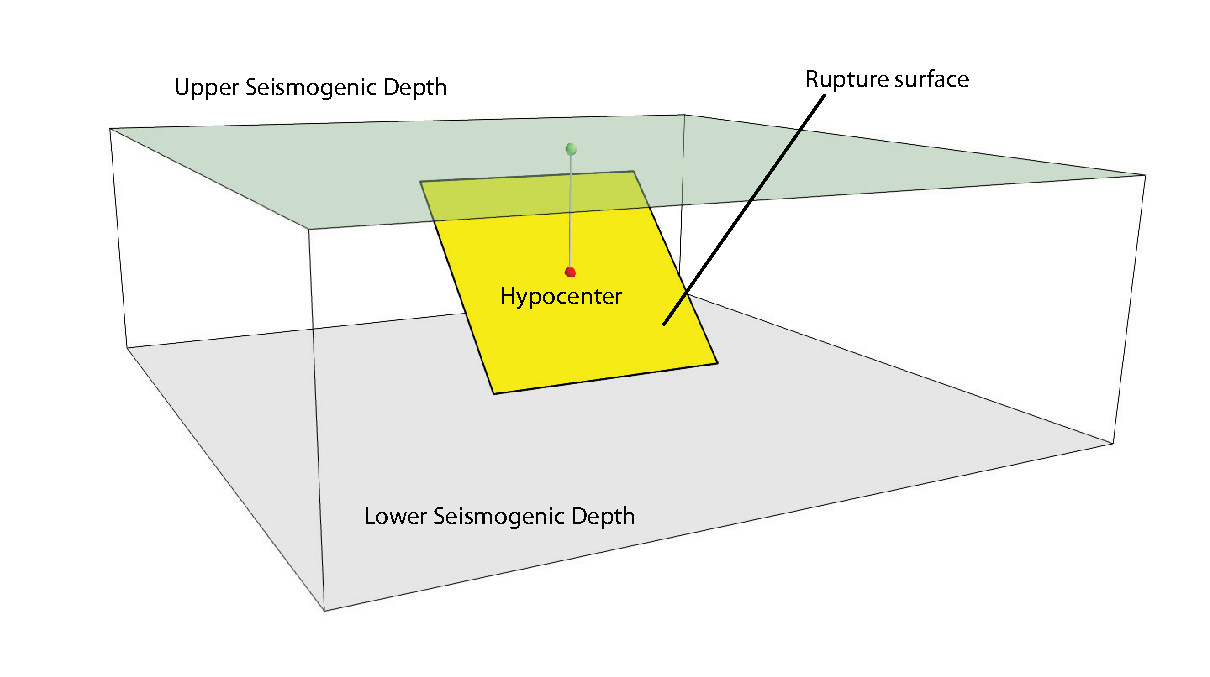
\includegraphics[width=10cm]{figures/hazard/single_rupture.pdf}
	\end{figure}}
}


\newglossaryentry{fragilityfunction}{
	name=fragility function,
	description={the probability of exceeding a set of limit states, given
	an intensity measure level. These functions can be discrete or continuous}
}


\newglossaryentry{fragilitymodel}{
	name=fragility model,
	description={A set of \glspl{vulnerabilityfunction} used to model the
	fragility of all the \glspl{asset} in the \gls{exposuremodel}}
}


\newglossaryentry{frequencymagnitudedistribution}{
	name=frequency-magnitude distribution,
	description={See \gls{mfd}}
}



% ------- G

\newacronym{acr:gem}{GEM}{Global Earthquake Model}
\newacronym{acr:gmf}{GMF}{Ground Motion Field}
\newacronym{acr:gmpe}{GMPE}{Ground Motion Prediction Equation}
\newacronym{acr:gmlt}{GMLT}{Ground Motion Logic Tree (see \gls{groundmotionlogictree}}


\newglossaryentry{gridsource}{
	name=grid source,
	description={A source typology usually adopted to model distributed
	seismicity. It is routinely produced by a seismicity smoothing algorithm (one
	of the most famous algorithm is the one proposed by \citet{frankel1995})}
}


\newglossaryentry{groundmotionfield}{
	name=ground-motion field,
	description={An object describing the geographic distribution around a
	rupture of a ground motion intensity measure}
}


\newglossaryentry{groundmotionfieldcalc}{
	name=ground-motion field calculator,
	description={An \gls{acr:oqe} calculator that given a rupture computes the
	geographic distribution of a ground motion intensity parameter. Currently
	OQ can generate ground motion fields using a \gls{acr:gmpe}}
}


\newglossaryentry{groundmotionlogictree}{
	name=ground-motion logic tree,
	description={A method used to systematically describe the epistemic
	uncertainties related to the ground motion models used in the computation
	of hazard using a specific \gls{pshainputmodel}}
}


\newglossaryentry{groundmotionmodel}{
	name=ground-motion model,
	description={An object that given a rupture with specific properties
	computes the expected ground motion at the given site. In simplest case a
	ground motion model corresponds to a \gls{groundmotionpredictioneq}. In
	case of complex PSHA input models, the produced ground motion models
	contains a set of \glspl{acr:gmpe}, one for each tectonic region considered}
}


\newglossaryentry{groundmotionparameter}{
	name=ground-motion parameter,
	description={A scalar or vector quantity describing a relevant property
	of the shaking such as intensity (e.g. PGA or Spectral Acceleration)
	or duration, equivalent number of cycles  \citep[see for
	example][]{hancock2005})}
}


\newglossaryentry{groundmotionpredictioneq}{
	name=ground-motion prediction equation,
	description={An equation that - given some fundamental parameters
	characterizing  the source, the propagation path and the site (in the
	simplest  case magnitude, distance and V$_\text{S,30}$) - computes the
	value $GM$ of a (scalar) ground motion intensity parameter}
}


\newglossaryentry{groundmotionsystem}{
	name=ground-motion system,
	description={An object containing a list of \gls{groundmotionlogictree}}
}



% ------- I

\newglossaryentry{initialseismicsourceinputmodel}{
	name=initial seismic source input model,
	description={It is the ensable of information needed to fully describe
	the seismic sources composing a seismic source input model. The
	initial seismic source input model is included in the first branching
	level of a seismic source logic tree}
}


\newglossaryentry{insuredlosses}{
	name=insured losses,
	description={Fraction of the ground-up losses that can be covered by the
	insurance industry, according to a certain policy}
}

\newacronym{acr:irmt}{IRMT}{}
\newglossaryentry{irmt}{
	name=Integrated Risk Modelling Toolkit,
	description={A plugin for QGIS which includes tools to run the \gls{oqe},
	to visualize hazard and risk results, to develop composite indicators
	and integrate them with physical risk estimations, and to predict building
	recovery times following an earthquake.
	This plugin was designed as a collaborative effort between the
	GEM Foundation and the Center for Disaster Management and Risk Reduction
	Technology, and it has been developed by the GEM Foundation.}
}

\newglossaryentry{investigationtime}{
	name=investigation time,
	description={The time interval considered to calculate hazard; usually
	it corresponds to 50 years}
}



% ------- L

\newglossaryentry{limit}{
	name=limit,
	description={A parameter used in the calculation of insured losses that
	establishes the maximum economic amount that can be covered by the insurance
	industry, according to a certain insurance policy}
}


\newglossaryentry{logictree}{
	name=logic tree,
	description={Data structure used to systematically describe uncertainties
	on parameters and models used in a PSHA study}
}


\newglossaryentry{logictreeprocessor}{
	name=logic tree processor,
	description={An OQ calculator that takes the PSHA Input Model and creates
	many realisations of a \gls{seismicsourcemodel} and of a
	\gls{groundmotionmodel}}
}


\newacronym{acr:ltmcs}{LTMCS}{Logic Tree Monte Carlo Sampler}

%------------M

\newglossaryentry{msr}{
	name=magnitude-scaling relationship,
	description={An empirical relationship linking the magnitude with a
	parameter  describing the size of the corresponding rupture (e.g. the
	area  of the rupture or the rupture length)}
}


\newacronym{acr:mfd}{MFD}{Magnitude-Frequency Distribution}
\newglossaryentry{mfd}{
	name=magnitude-frequency distribution,
	description={A distribution describing the frequency of earthquakes with
	a specific magnitude. It can be continuous or discrete. One frequency-
	magnitude distribution frequently adopted in \gls{acr:psha} is the double
	truncated Gutenberg-Richter distribution}
}

%---------------N
\newglossaryentry{nonparametricsource}{
    name=non-parametric source,
    description={A source typology in which the earthquake rupture forecast is
    described explicitly by a set of ruptures and the corresponding
    probabilities of occurrence}
}



% ------- N

\newacronym{acr:nrml}{NRML}{Natural hazards' Risk Markup Language}
\newglossaryentry{nrml}{
	name=Natural hazards' Risk Markup Language,
	description={A markup language similar to XML, which specifies a number
	of standardised schemas to represent various input models used for
	\gls{acr:oqe} calculations and output files generated by \gls{acr:oqe}
	calculations
	}
}



% ------- O

\newacronym{acr:hazlib}{oq-hazardlib}{OpenQuake hazard library}


\newglossaryentry{opensha}{
	name=OpenSHA,
	description={OpenSHA is an open-source, advanced Java-based platform
	for conducting Seismic Hazard Analysis - (see
	\href{http://opensha.org}{OpenSHA website})}
}


\newacronym{acr:oqe}{oq-engine}{OpenQuake-engine}
\newacronym{acr:oqe17}{oq-engine 1.7}{OpenQuake-engine v1.7}
\newacronym{acr:oqe18}{oq-engine 1.8}{OpenQuake-engine v1.8}
\newacronym{acr:oqe19}{oq-engine 1.9}{OpenQuake-engine v1.9}
\newacronym{acr:oqe20}{oq-engine 2.0}{OpenQuake-engine v2.0}
\newacronym{acr:oqe21}{oq-engine 2.1}{OpenQuake-engine v2.1}
\newacronym{acr:oqe22}{oq-engine 2.2}{OpenQuake-engine v2.2}
\newacronym{acr:oqe23}{oq-engine 2.3}{OpenQuake-engine v2.3}
\newacronym{acr:oqe24}{oq-engine 2.4}{OpenQuake-engine v2.4}
\newacronym{acr:oqe25}{oq-engine 2.5}{OpenQuake-engine v2.5}
\newacronym{acr:oqe26}{oq-engine 2.6}{OpenQuake-engine v2.6}
\newacronym{acr:oqe27}{oq-engine 2.7}{OpenQuake-engine v2.7}
\newacronym{acr:oqe28}{oq-engine 2.8}{OpenQuake-engine v2.8}
\newacronym{acr:oqe29}{oq-engine 2.9}{OpenQuake-engine v2.9}
\newacronym{acr:oqe30}{oq-engine 3.0}{OpenQuake-engine v3.0}
\newacronym{acr:oqe31}{oq-engine 3.1}{OpenQuake-engine v3.1}
\newacronym{acr:oqe32}{oq-engine 3.2}{OpenQuake-engine v3.2}
\newacronym{acr:oqe33}{oq-engine 3.3}{OpenQuake-engine v3.3}
\newacronym{acr:oqe34}{oq-engine 3.4}{OpenQuake-engine v3.4}



% ------- P

\newacronym{acr:pga}{PGA}{Peak Ground Acceleration}
\newacronym{acr:pgv}{PGV}{Peak Ground Velocity}

\newacronym[description={\glslink{psha}{Probabilistic Seismic Hazard
	Analysis}}]{acr:psha}{PSHA}{Probabilistic Seismic Hazard Analysis}


\newglossaryentry{pointsource}{
	name=point source,
	description={The elemental source typology used in the \glsdesc{acr:oqe} to
	model distributed seismicity}
}


\newglossaryentry{pshainputmodel}{
	name=PSHA input model,
	description={An object containing the information necessary to describe
	the seismic source and the ground motion models - plus the related
	epistemic uncertainties}
}


\newglossaryentry{psha}{
	name=probabilistic seismic hazard analysis,
	description={A methodology to compute seismic hazard by taking into
	account the potential contributions coming from all the sources of
	engineering importance for a specified site}
}



% ------- R

\newacronym{acr:risklib}{oq-risklib}{OpenQuake risk library}


\newacronym{acr:rrup}{$\text{r}_{\text{rup}}$}{closest distance between the
	site and rupture}


\newglossaryentry{rupture}{
	name=earthquake rupture,
	description={A 3D surface - representing a portion or the entire fault
	surface - over which a slip event (i.e. an earthquake) occurs}
}


\newglossaryentry{rupturemodel}{
	name=rupture model,
	description={An object containing the information necessary to describe
	a \gls{rupture}, such as magnitude, hypocenter location, strike, dip, 
	rake, and seismogenic depths}
}


\newglossaryentry{ruptureaspectratio}{
	name=rupture aspect ratio,
	description={The ratio between the lenght and the width of an
	earthquake rupture}
}


\newglossaryentry{rake}{
	name=rake,
	description={The rake is the direction in which a hanging wall block moves
	during a rupture, measured relative to fault strike on the plane of the
	fault}
}



% ------- S

\newacronym{acr:ssha}{SSHA}{Scenario Based Seismic Hazard Analysis}


\newglossaryentry{scenariohazard}{
	name=scenario based seismic hazard analysis,
	plural=scenario based seismic hazard analyses,
	description={An analyis of seismic hazard based on the selection of
	one or a few ruptures and the computation of the expected ground
	motion at a set of sites using a \gls{gmpe} accounting ground motion
	variability}
}


\newglossaryentry{seismicityhistory}{
	name=seismicity history,
	plural=seismicity histories,
	description={An object containing a set ruptures representative of the
	possible seismicity generated by the sources in a
	\gls{seismicsourcemodel} during the investigation time $t$}
}


\newglossaryentry{seismicityrate}{
	name=seismicity rate,
	description={Number of events per unit of time (if not better
	specified, the definition of a seismicity rate generally presumes a time
	independent}
}


\newglossaryentry{seismicsourcedata}{
	name=seismic source data,
	description={An object containing the information necessary to
	completely describe a \gls{acr:psha} seismic source i.e. seismic source
	type, position, geometry and seismicity occurrence model}
}


\newglossaryentry{seismicsourcelogictree}{
	name=seismic source logic tree,
	description={Logic tree structure defined to describe in structured and
	systematic way the epistemic uncertainties characterizing the seismic
	source model. The first branching level in the logic tree by definition
	contains one or several alternative \gls{initialseismicsourceinputmodel}}
}


\newacronym{acr:ssim}{SSIM}{Seismic Source Input Model}


\newglossaryentry{seismicsourceinputmodel}{
	name=seismic source input model,
	description={An object containing a list of \gls{seismicsourcedata}. In
	the \glsdesc{acr:oqe} a seismic source model doesn't contain epistemic
	uncertainty}
}


\newglossaryentry{seismicsource}{
	name=seismic source,
	description={An object that can generate}}


\newacronym{acr:ssm}{SSM}{Seismic Source Model}
\newglossaryentry{seismicsourcemodel}{
	name=seismic source model,
	description={An object containing a list of \glspl{seismicsource}
	objects}
}


\newacronym{acr:scec}{SCEC}{Southern California Earthquake Center}


\newglossaryentry{seismicsourcesystem}{
	name=seismic source system,
	description={An object containing a list of
	\glspl{initialseismicsourceinputmodel} and the
	\gls{seismicsourcelogictree}}
}


\newglossaryentry{simplefaultsource}{
	name=simple fault source,
	description={A source typology usually adopted to model shallow
	structures with an uncomplicated geometry}
}


\newacronym{acr:ses}{SES}{Stochastic Event Set}
\newglossaryentry{stochasticeventset}{
	name=stochastic event set,
	description={An object containing one or many \glspl{seismicityhistory}}
}


\newglossaryentry{strike}{
	name=strike,
	description={The strike direction correspond to the angle between the
	north and the direction you take so that when you walk along the
	\gls{faulttrace} the fault dips on your right}
}


\newacronym{acr:sa}{S$_a$}{Spectral Acceleration}



% ------- T

\newglossaryentry{tag}{
	name=tag,
	plural=tags,
	description={Scheme used to specify attributes for the \glspl{asset}.
	Attributes for an \gls{asset} could include the state, county, zip-code,
	city, occupancy, CRESTA ID, or other such markers that could be used 
	in the post-processing stage of a risk calculation to aggregate
	results for each tag.}
}

\newglossaryentry{taxonomy}{
	name=taxonomy,
	plural=taxonomies,
	description={Scheme used to classify the \glspl{asset}. For buildings, a
	classification scheme has been proposed by \gls{acr:gem} which considers a
	number of attributes including lateral load resisting system and its
	material, height, year of construction. The taxonomy is currently used to
	link the \glspl{asset} in the \gls{exposuremodel} to the relevant
	\gls{vulnerabilityfunction} or \gls{fragilityfunction}}
}


\newglossaryentry{tectonicregion}{
	name=tectonic region,
	description={A area on the topographic surface that can be considered
	homogeneous in terms of tectonic properties such as the prevalent
	seismogenic properties and/or the seismic wave propagation properties}
}


\newglossaryentry{temporaloccurrencemodel}{
	name=temporal occurrence model,
	description={Usually a probabilistic model giving the probability of
	occurrence of an event in a specified \gls{investigationtime}}
}



% ------- U

\newacronym{acr:usgs}{USGS}{United States Geological Survey}



% ------- V

\newglossaryentry{vulnerabilityfunction}{
	name=vulnerability function,
	description={A function that describes the probability distribution of
	loss ratio, conditioned on an intensity measure level. Currently only
	discrete vulnerability functions are supported}
}


\newglossaryentry{vulnerabilitymodel}{
	name=vulnerability model,
	description={A set of \glspl{vulnerabilityfunction} used to model the
	physical vulnerability of all the \glspl{asset} in the \gls{exposuremodel}}
}


\newglossaryentry{acr:vs30}{
	name=V$_{S,30}$,
	description={Average shear wave velocity of the materials in the uppermost
	30m of the soil column}
}
 % ---------------------------------------- Load glossary -

%-------------------------------------------------------------------------------
%  COVER PAGE
%-------------------------------------------------------------------------------

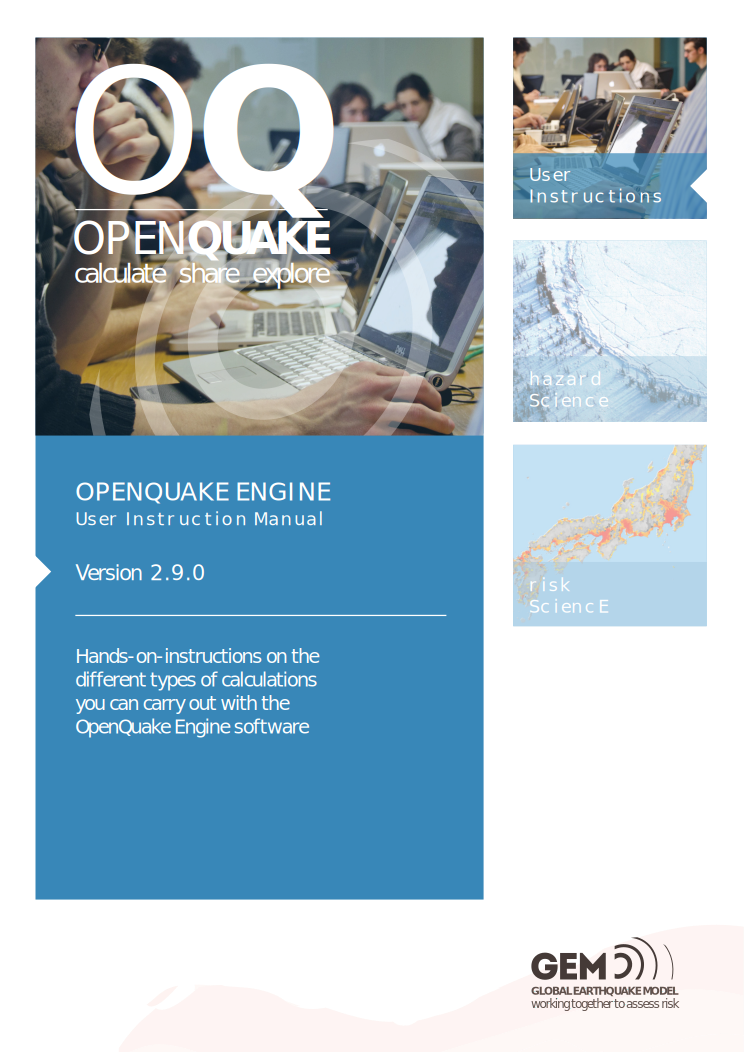
\includepdf[pages=-]{figures/oq_manual_cover.pdf}

%-------------------------------------------------------------------------------
%  TITLE PAGE
%-------------------------------------------------------------------------------

\begingroup
\thispagestyle{empty}
\begin{center}
\par\normalfont\fontsize{15}{15}\sffamily\selectfont
\textcolor{oqblue}{OpenQuake: calculate, share, explore}
\vspace*{9cm}
\par\bfseries\fontsize{35}{35}\sffamily\selectfont
\textcolor{gembrown}{The OpenQuake-engine\\User Instruction Manual}\par
\vspace*{9cm}
\par\normalfont\fontsize{15}{15}\sffamily\selectfont
\href{http://globalquakemodel.org/openquake/}{\textcolor{oqblue}{globalquakemodel.org/openquake}}
\end{center}
\endgroup

%-------------------------------------------------------------------------------
%  COPYRIGHT PAGE
%-------------------------------------------------------------------------------

\newpage
~\vfill
\thispagestyle{empty}

\noindent
   \textbf{Authors} \\
   Marco Pagani$^1$, Vitor Silva$^1$,
   Anirudh Rao$^1$, Michele Simionato$^1$, Robin Gee$^1$\hfill \\
   \hfill \\
   \textbf{Authors on previous versions} \\
   Helen Crowley$^2$, Damiano Monelli, Graeme Weatherill$^3$\hfill \\
   \hfill \\
   \small
   \begin{tabular}{p{4cm}p{4cm}p{4cm}}
   $^1$ GEM Foundation \hfill \newline
   via Ferrata, 1 \hfill \newline
   20133 Pavia \hfill \newline
   Italy \hfill \newline
   &
   $^2$ EUCENTRE \hfill \newline
   via Ferrata, 1 \hfill \newline
   20133 Pavia \hfill \newline
   Italy \hfill \newline
   &
   $^3$ GFZ \hfill \newline
   Helmholtzstraße 6/7 \hfill \newline
   14467 Potsdam \hfill \newline
   Germany \hfill \newline
   \end{tabular} \hfill \newline
   %
   Email address for all current authors:\hfill\\
   $<$name.surname$>$@globalquakemodel.org\hfill\\
   \normalsize

\noindent
   {\textbf{Citation}} \hfill \\
   Please cite this document as: \hfill \\
   GEM (2017). The OpenQuake-engine User Manual.
   \textit{Global Earthquake Model (GEM) Technical Report 2017-11.\\
   doi: 10.13117/GEM.OPENQUAKE.MAN.ENGINE.2.8/01, 192 pages.} \hfill \\
\noindent \hfill\\
\noindent
   {\bf{Disclaimer}} \hfill \\
   The OpenQuake-engine User Manual is distributed in the hope that it will be
   useful, but without any warranty: without even the implied warranty of
   merchantability or fitness for a particular purpose. While every precaution
   has been taken in the preparation of this document, in no event shall the
   authors of the Manual and the GEM Foundation be liable to any party for
   direct, indirect, special, incidental, or consequential damages, including
   lost profits, arising out of the use of information contained in this
   document or from the use of programs and source code that may accompany it,
   even if the authors and GEM Foundation have been advised of the possibility
   of such damage. The Manual provided hereunder is on as ``as is'' basis, and
   the  authors and GEM Foundation have no obligations to provide maintenance,
   support, updates, enhancements, or modifications. \hfill \\
\noindent \hfill\\
\noindent
   {\bf{License}} \hfill \\
   This Manual is distributed under the Creative Commons License  Attribution-
   NonCommercial-ShareAlike 4.0 International
   (\href{http://creativecommons.org/licenses/by-nc-sa/4.0/} {CC BY-NC-SA
   4.0}). You can download this Manual and share it with others as long as you
   provide proper credit, but you cannot change it in any way or use it
   commercially.\hfill \\

\noindent \copyright\ \textsc{2013--2017 GEM Foundation}\\
\noindent \textit{Sixteenth printing, November 2017} % Printing/edition date

%-------------------------------------------------------------------------------
%  TABLE OF CONTENTS
%-------------------------------------------------------------------------------

\chapterimage{figures/chapter_head.pdf} % Table of contents heading image
\pagestyle{empty} % No headers
\tableofcontents % Print the table of contents itself
\cleardoublepage % Forces the first chapter to start on the right
\pagestyle{fancy} % Print headers again

%-------------------------------------------------------------------------------
%  FOREWORD
%-------------------------------------------------------------------------------
\chapterimage{figures/chapter_head.pdf} % Chapter heading image
\chapter*{Preface}
\addcontentsline{toc}{chapter}{Preface}
The goal of this manual is to provide a comprehensive and transparent
description of the features of the \glsdesc{acr:oqe24}. This manual is
designed to be readable by someone with basic understanding of Probabilistic
Seismic Hazard and Risk Analysis, but no previous knowledge of the
\glsdesc{acr:oqe} is assumed.

The \glsdesc{acr:oqe} is an effort promoted and actively developed by the
\glsdesc{acr:gem}, a public-private partnership initiated by the
Global Science Forum of the Organisation for Economic Co-operation and Development
(OECD)\footnote{A short description of the process promoted by OECD is available here:\\\href{http://www.oecd.org/science/sci-tech/theglobalearthquakemodelgem.htm}{http://www.oecd.org/science/sci-tech/theglobalearthquakemodelgem.htm}}.

The \glsdesc{acr:oqe} is the result of an effort carried out jointly by the
Information Technology and Scientific teams working at the \gls{acr:gem} Secretariat.
It is freely distributed under an Affero GPL license
(\href{http://www.gnu.org/licenses/agpl-3.0.html}{http://www.gnu.org/licenses/agpl-3.0.html}).

%-------------------------------------------------------------------------------
%  THE MANUAL
%-------------------------------------------------------------------------------

% ------------------------------------------------------- Part I: Introduction -
\part{Introduction}
\label{part:introduction}
\chapterimage{figures/chapter_head.pdf} % Chapter heading image
\chapter{OpenQuake-engine Background}
   \label{chap:intro}
	OpenQuake-engine is the seismic hazard and risk calculation software developed by
the \glsdesc{acr:gem}. By following current standards in software
developments like test-driven development and continuous integration, the
\glsdesc{acr:oqe} aims at becoming an open, and community-driven tool for
seismic hazard and risk analysis.

The source code of the \glsdesc{acr:oqe} is available on a public web-based
repository at the following address:
\href{http://github.com/gem/oq-engine}{http://github.com/gem/oq-engine}.

The \glsdesc{acr:oqe} is available for the Linux, macOS, and Windows
platforms. It can be installed in several different ways. The following page
provides a handy guide for users to choose the most appropriate installation
method depending on their intended use cases:

\href{https://github.com/gem/oq-engine/blob/engine-3.0/doc/installing/overview.md}{https://github.com/gem/oq-engine/blob/engine-3.0/doc/installing/overview.md}.

An \gls{acr:oqe} analysis is launched from the command line of a terminal.

A schematic list of the options that can be used for the execution of the
\gls{acr:oqe} can be obtained with the following command:

\begin{minted}[fontsize=\footnotesize,frame=single,bgcolor=lightgray]{shell-session}
user@ubuntu:~\$ oq engine --help
\end{minted}

The result is the following:
\inputminted[firstline=1,fontsize=\footnotesize,frame=single]{shell-session}{oqum/help.txt}


% ----------------------------------------------------- Part II: Hazard Module -
\thispagestyle{empty}
\part{Hazard}

\chapterimage{figures/chapter_head.pdf} % Chapter heading image
\chapter{Introduction to the Hazard Module}
   \label{chap:hazintro}
	\index{OpenQuake-engine!Hazard}

The hazard component of the \glsdesc{acr:oqe} builds on top of the
\gls{acr:hazlib}, a Python-based library containing tools for PSHA
calculations.

The web repository of this library is available at the following address:\\
\href{http://github.com/gem/oq-hazardlib}{http://github.com/gem/oq-hazardlib}.

In this section we briefly illustrate the main properties of the hazard
component of the \glsdesc{acr:oqe}. In particular, we will describe the main typologies of sources supported and the main calculation workflows available.


\section{Source typologies}
\index{Source type}
\label{sec:source_typologies}
An \glsdesc{acr:oqe} \gls{seismicsourceinputmodel} contains a list of sources
belonging to a finite set of possible typologies. Each source type is defined
by a set of parameters - called source data - which are used to specify the
source geometry and the properties of seismicity occurrence.

Currently the \glsdesc{acr:oqe} supports the following source types:

\begin{itemize}

    \item Sources for modelling distributed seismicity:

    \begin{itemize}

        \item \Gls{pointsource} - The elemental source type used to model
        distributed seismicity. Grid and area sources (described below) are
        different containers of point sources.

        \item \Gls{areasource} - So far, the most frequently adopted source
        type in national and regional PSHA models.

        \item \Gls{gridsource} - A replacement for area sources admitting
        spatially variable seismicity occurrence properties.

    \end{itemize}

    \item Fault sources with floating ruptures:

    \begin{itemize}

        \item \Gls{simplefaultsource} - The simplest fault model in the
        \glsdesc{acr:oqe}. This source is habitually used to describe shallow
        seismogenic faults.

        \item \Gls{complexfaultsource} - Often used to model subduction
        interface sources with a complex geometry.

    \end{itemize}

    \item Fault sources with ruptures always covering the entire fault surface:

    \begin{itemize}

        \item \Gls{charfaultsource} - A typology of source where ruptures
        always fill the entire fault surface.
        
        \item \Gls{nonparametricsource} - A typology of source representing
        a collection of ruptures, each with their associated probabilities
        of 0, 1, 2 ... occurrences in the investigation time

    \end{itemize}

    \item Sources for representing individual earthquake ruptures
    
    \begin{itemize}
        \item Planar fault rupture - an individual fault rupture represented as a single rectangular plane
        \item Multi-planar fault rupture - an individual rupture represented as a collection of rectangular planes
        \item Simple fault rupture - an individual fault rupture represented as a simple fault surface
        \item Complex fault rupture - an individual fault rupture represented as a complex fault surface
    \end{itemize}

\end{itemize}

The \glsdesc{acr:oqe} contains some basic assumptions for the definition of
these source typologies:

\begin{itemize}

    \item In the case of area and fault sources, the seismicity is
    homogeneously distributed over the source;

    \item Seismicity temporal occurrence follows a Poissonian model.

\end{itemize}

The above sets of sources may be referred to as ``parametric'' sources, that
is to say that the generation of the \Gls{earthquakeruptureforecast} is done
by the OpenQuake engine based on the parameters of the sources set by the
user. In some cases, particularly if the user wishes for the temporal
occurrence model to be non-Poissonian (such as the lognormal or Brownian
Passage Time models) a different type of behaviour is needed. For this
OpenQuake-engine supports a \Gls{nonparametricsource} in which the
\Gls{earthquakeruptureforecast} is provided explicitly by the user as a set of
ruptures and their corresponding probabilities of occurrence.

\subsection{Source typologies for modelling distributed seismicity}
\subsubsection{Point sources}
\label{subsubsec:point_sources}
\index{Source type!point}
\index{Point source|see{Source type}}

\begin{figure}[!ht]
\centering
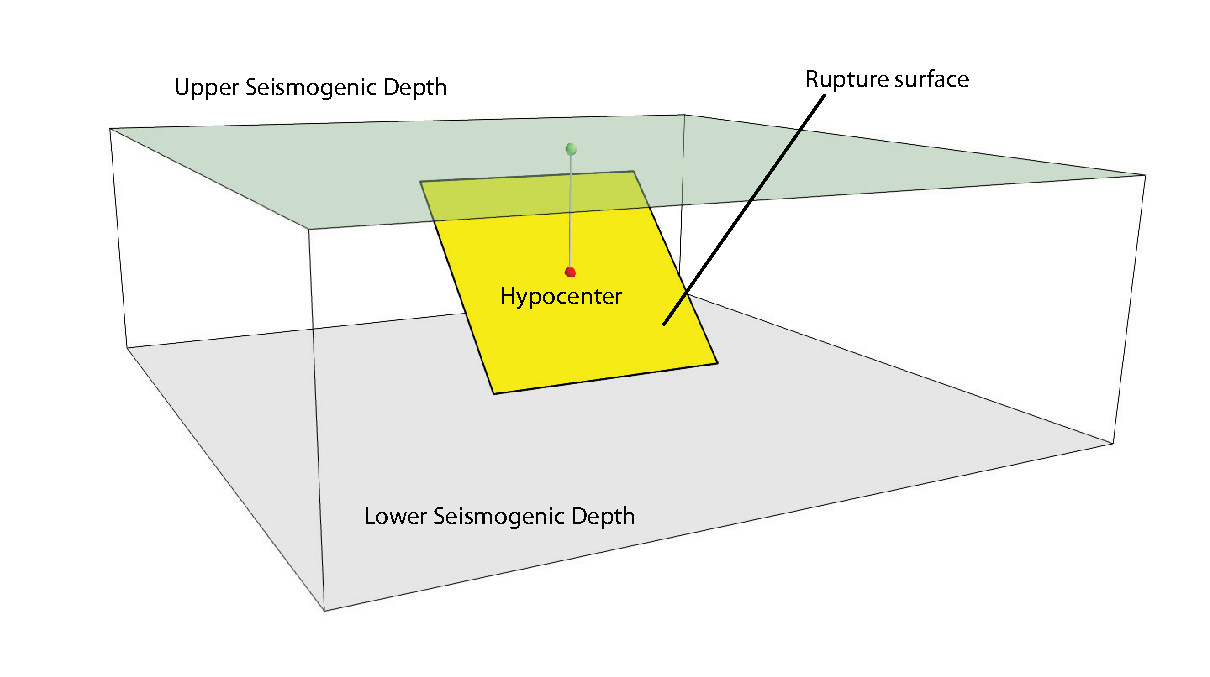
\includegraphics[width=10cm]{figures/hazard/single_rupture.pdf}
\caption{Single rupture}
\label{fig:single_rupture}
\end{figure}

The point source is the elemental source type adopted in the OpenQuake-engine
for modelling distributed seismicity. The \glsdesc{acr:oqe} always performs
calculations considering finite ruptures, even in the case of point sources.

These are the basic assumptions used to generate ruptures with point sources:

\begin{itemize}

    \item Ruptures have a rectangular shape

    \item Rupture hypocenter is located in the middle of the rupture

    \item Ruptures are limited at the top and at the bottom by two planes
    parallel to the sea level and placed at two characteristic
    depths named upper and lower seismogenic depths, respectively (see
    Figure~\ref{fig:single_rupture})

\end{itemize}

\paragraph{Source data}

For the definition of a point source the following parameters are required
(Figure~\ref{fig:single_rupture} shows some of the parameters described
below, together with an example of the surface of a generated rupture):

\begin{itemize}

    \item The coordinates of the point (i.e. longitude and latitude) [decimal
    degrees]

    \item The upper and lower seismogenic depths [km]

    \item One \gls{mfd}

    \item One magnitude-scaling relationship

    \item The rupture aspect ratio

    \item A distribution of nodal planes i.e. one (or several) instances
    of the following set of parameters:

    \begin{itemize}
        \item \gls{strike} [degrees]
        \item \gls{dip} [degrees]
        \item \gls{rake} [degrees]
    \end{itemize}

\item A magnitude independent depth distribution of hypocenters [km].

\end{itemize}

Figure~\ref{fig:point_source_multiple_ruptures} shows ruptures generated by a
point source for a range of magnitudes. Each rupture is centered on the
single hypocentral position admitted by this point source. Ruptures are
created by conserving the area computed using the specified magnitude-area
scaling relatioship and the corresponding value of magnitude.

\begin{figure}[ht!]
\centering
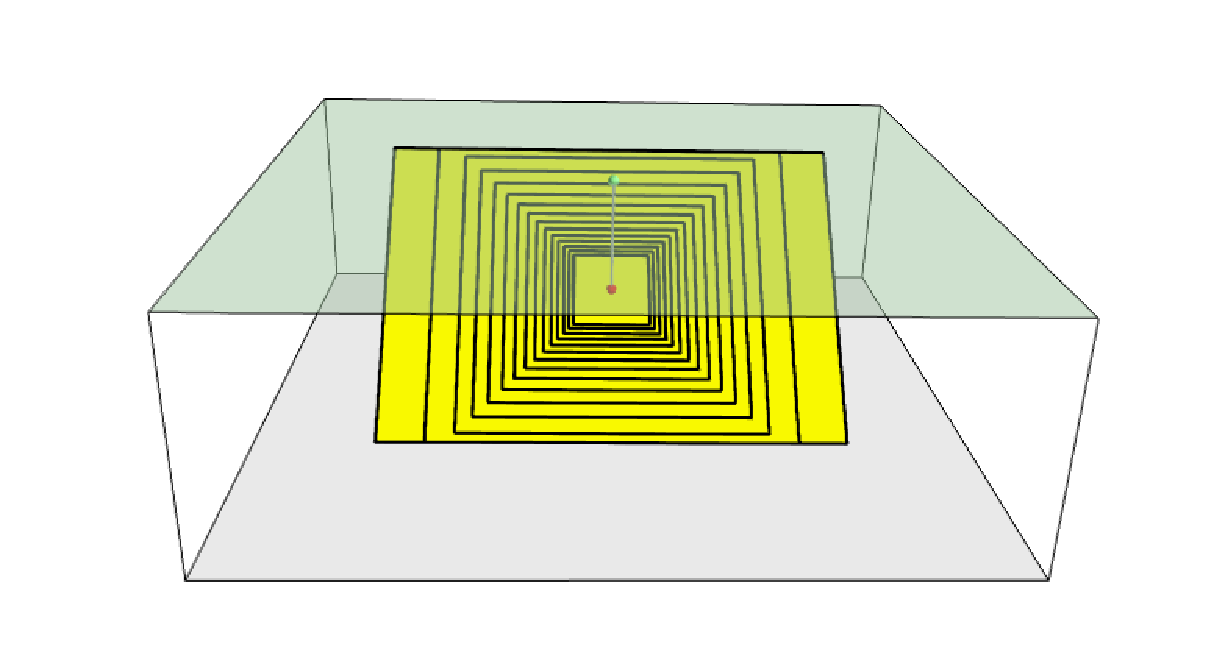
\includegraphics[width=10cm]{figures/hazard/point_source_multiple_ruptures.pdf}
\caption{Point source with multiple ruptures. Note the change in the aspect
ratio once the rupture width fills the entire seismogenic layer.}
\label{fig:point_source_multiple_ruptures}
\end{figure}

Below we provide the excerpt of an .xml file used to describe the properties of a point source. Note that in this example, ruptures occur on two possible nodal planes and two hypocentral depths. Figure~\ref{fig:point_source_ruptures} shows the ruptures generated by the point source.

\begin{listing}[htbp]
  \inputminted[firstline=1,firstnumber=1,fontsize=\footnotesize,frame=single,linenos,bgcolor=lightgray]{xml}{oqum/hazard/verbatim/input_point_source.xml}
  \caption{Example point source}
  \label{page:point_source_nrml}
\end{listing}

%The red part shows the the parameters used to describe the geometry of the point source, the blue part is the description of the magnitude-frequency distribution, the green text shows the nodal plane distribution and the text in magenta illustrates the hypocentral depth distribution.

%The text in black describes the parameters needed to generate the ruptures such as the \gls{msr} and the aspect ratio.



\begin{figure}[!ht]
\centering
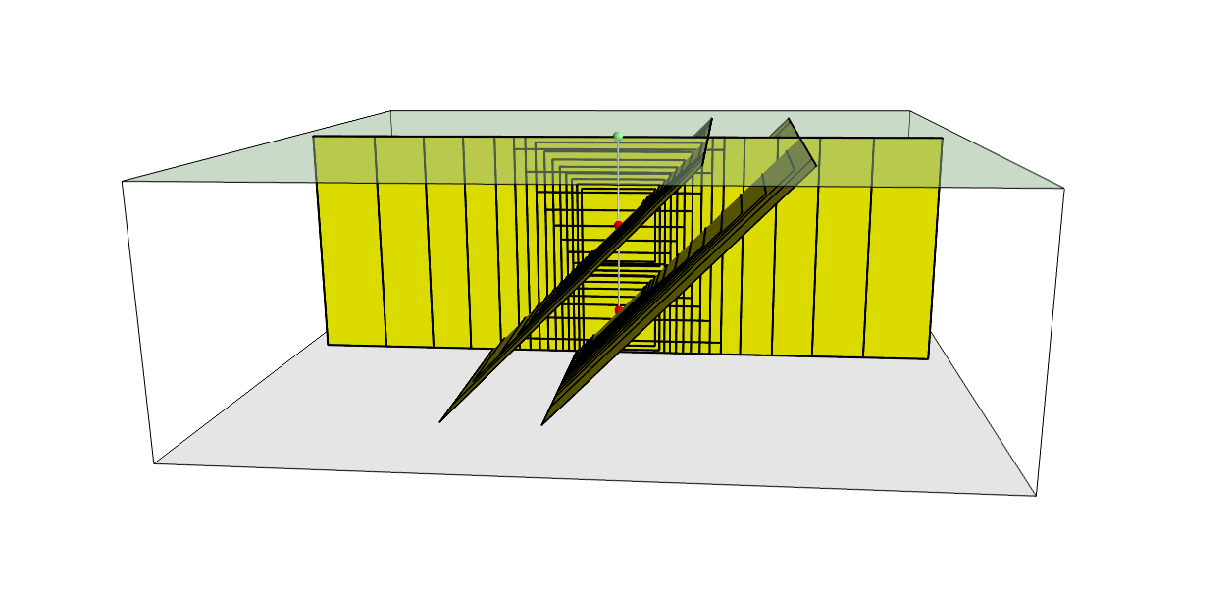
\includegraphics[width=10cm]{figures/hazard/pointsrc_2strike_2hypodep.pdf}
\caption{Ruptures produced by the source created using the information 
in the example .xml file described on page~\pageref{page:point_source_nrml}.}
\label{fig:point_source_ruptures}
\end{figure}

\subsubsection{Grid sources}
\label{subsubsec:grid_sources}
\index{Source type!grid}
\index{Grid source|see{Source type}}

A \gls{gridsource} is simply a collection of point sources distributed over a regular grid (usually equally spaced in longitude and latitude). In \gls{psha} a grid source can be considered a model alternative to area
sources, since they both model distributed seismicity. Grid sources are generally used to reproduce more faithfully the spatial pattern of seismicity depicted by the earthquakes occurred in the past; in
some models (e.g. \citet{petersen2008}) only events of low and intermediate magnitudes are considered. They are frequently, though not always, computed using seismicity smoothing algorithms \citep[][amongst many others]{frankel1995,woo1996}.

The use of smoothing algorithms to produce grid sources brings some
advantages compared to area sources, since (1) it removes most of the
unavoidable degree of subjectivity due to the definition of the geometries of the area sources and (2) it produces a spatial pattern of seismicity that is usually closer to what observed in the reality. Nevertheless, in many cases smoothing algorithms require an a-priori definition of some setup parameters that expose the calculation to a certain degree of partiality.

Grid sources are modeled in \gls{acr:oqe} simply as a set of point sources; in other words, a grid source is just a long list of point sources specified as described in the previous section (see page
\pageref{subsubsec:point_sources}).

\subsubsection{Area sources}
\label{subsubsec:area_sources}
\index{Source type!area}
\index{Area source|see{Source type}}

Area sources are usually adopted to describe the seismicity occurring over wide areas where the identification and characterization - i.e. the
unambiguous definition of position, geometry and seismicity occurrence
parameters - of single fault structures is difficult.

From a computation standpoint, area sources are comparable to grid sources since they are both represented in the engine by a list of point sources.

The \gls{acr:oqe} using the source data parameters (see below) creates an
equally spaced in distance grid of point sources where each point has the same seismicity occurrence properties (i.e. rate of events generated).

Below we provide a brief description of the parameters necessary to completely describe an area source.

\paragraph{Source data}

\begin{itemize}

    \item A polygon defining the external border of the area (i.e. a list of
    Longitude-Latitude [degrees] tuples) The current version of the OQ-engine doesn't
    support the definition of internal borders.

    \item The upper and lower seismogenic depths [km]

    \item One \gls{mfd}

    \item One \gls{msr}

    \item The rupture aspect ratio

    \item A distribution of nodal planes i.e. one (or several) instances of
    the following set of parameters

    \begin{itemize}
        \item \gls{strike} [degrees]
        \item \gls{dip} [degrees]
        \item \gls{rake} [degrees]
    \end{itemize}

    \item A magnitude independent depth distribution of hypocenters [km].

\end{itemize}

Below we provide the excerpt of an .xml file used to describe the properties of an area source. The ruptures generated by the area source described in the example are controlled by two nodal planes and have hypocenters at localized at two distinct depths.

\begin{listing}[htbp]
  \inputminted[firstline=1,firstnumber=1,fontsize=\footnotesize,frame=single,linenos,bgcolor=lightgray]{xml}{oqum/hazard/verbatim/input_area_source.xml}
  \caption{Example area source}
  \label{lst:area_source}
\end{listing}

%The red text describes the parameters used to describe the geometry of the area source; the blue part is the description of the magnitude-frequency distribution; the green text displays the nodal plane distribution; and the text in magenta illustrates the hypocentral depth distribution.

%The text in gray describes the parameters required to generate the ruptures such as the \gls{msr} and the aspect ratio.



\subsection{Fault sources with floating ruptures}
Fault sources in the \gls{acr:oqe} are classified according to the method
adopted to distribute ruptures over the fault surface. Two options are
currently supported:

\begin{itemize}

    \item With the first option, ruptures with a surface lower than the
    whole fault surface are floated so as to cover as much as possible
    homogeneously the fault surface. This model is compatible with all the
    supported magnitude-frequency distributions.

    \item With the second option, ruptures always fill the entire fault
    surface. This model is compatible with magnitude-frequency
    distributions similar to a characteristic model (\`{a} la
    \cite{schwartz1984}).

\end{itemize}

In this subsection we discuss the different fault source types that
support floating ruptures. In the next subsection we will illustrate the fault
typology available to model a characteristic rupturing behaviour.



\subsubsection{Simple faults}
\label{desc_simple_fault}
\index{Source type!fault!simple geometry}
\index{Simple fault|see{Source type}}

Simple Faults are the most common source type used to model shallow faults;
the ``simple'' adjective relates to the geometry description of the source
which is obtained by projecting the fault trace (i.e. a polyline) along a
characteristic dip direction.

The parameters used to create an instance of this source type are described
in the following paragraph.

\paragraph{Source data}

\begin{itemize}

    \item A horizontal \gls{faulttrace} (usually a polyline). It is a list of
    longitude-latitude tuples [degrees].

    \item A \gls{frequencymagnitudedistribution}

    \item A \gls{msr}

    \item A representative value of the dip angle (specified following
    the Aki-Richards convention; see \citet{aki2002}) [degrees]

    \item Rake angle (specified following the Aki-Richards convention;
    see \citet{aki2002}) [degrees]

    \item Upper and lower depth values limiting the seismogenic interval [km]

\end{itemize}

For near-fault probabilistic seismic hazard analysis, two additional
parameters are needed for characterising seismic sources:

\begin{itemize}

    \item A hypocentre list. It is a list of the possible hypocentral
    positions, and the corresponding weights, e.g., alongStrike="0.25"
    downDip="0.25" weight="0.25". Each hypocentral position is defined in
    relative terms using as a reference the upper left corner of the rupture
    and by specifying the fraction of rupture length and rupture width.

    \item A slip list. It is a list of the possible rupture slip directions
    [degrees], and their corresponding weights. The angle describing each slip
    direction is measured counterclockwise using the fault strike direction as
    reference.

\end{itemize}

In near-fault PSHA calculations, the hypocentre list and the slip list are
mandatory. The weights in each list must always sum to one. The available GMPE
which currently supports the near-fault directivity PSHA calculation in OQ-
engine is the ChiouYoungs2014NearFaultEffect GMPE developed  by
\citet{chiou2014update} (associated with an \texttt{Active Shallow Crust}
tectonic region type).

We provide two examples of simple fault source files. The first is an
excerpt of an xml file used to describe the properties of a simple fault
source and the second example shows the excerpt of an xml file used to
describe the properties of a simple fault source that can be used to perform a PSHA calculation taking into account directivity effects.

\begin{listing}[htbp]
  \inputminted[firstline=1,firstnumber=1,fontsize=\footnotesize,frame=single,linenos,bgcolor=lightgray]{xml}{oqum/hazard/verbatim/input_simple_fault.xml}
  \caption{Example simple fault}
  \label{lst:example_simple_fault}
\end{listing}
%\input{oqum/hazard/verbatim/input_simple_fault}
%\label{example_incremental_mfd}

%Below is an excerpt of a simple fault source xml file for near-fault directivity PSHA calculations:

%\begin{listing}[htbp]
\inputminted[firstline=1,firstnumber=1,fontsize=\footnotesize,frame=single,linenos,bgcolor=lightgray]{xml}{oqum/hazard/verbatim/input_simple_fault_directivity.xml}
\captionof{listing}{Example simple fault with added information to model directivity\label{lst:example_simple_fault_directivity}}

%\end{listing}

%\input{oqum/hazard/verbatim/input_simple_fault_directivity}

%As with the previous examples, the red text highlights the parameters used to specify the source geometry, the parameters in green describe the rupture mechanism, the text in blue describes the magnitude-frequency distribution and the gray text describes the rupture properties.



\subsubsection{Complex faults}
\label{desc_complex_fault}
\index{Source type!fault!complex geometry}
\index{Complex fault|see{Source type}}

A complex fault differs from simple fault just by the way the geometry of the
fault surface is defined and the fault surface is later created. The input
parameters used to describe complex faults are, for the most part, the same
used to describe the simple fault typology.

In the case of complex faults, the dip angle is not requested while the fault
trace is substituted by two fault edges limiting the top and bottom of the fault
surface. Additional curves lying over the fault surface can be specified to
complement and refine the description of the fault surface geometry.
Unlike the simple fault these edges are not required to be horizontal
and may vary in elevation, i.e. the upper edge may represent the intersection 
between the exposed fault trace and the topographic surface, where positive values
indicate below sea level, and negative values indicate above sea level.

Usually, we use complex faults to model intraplate megathrust faults such as
the big subduction structures active in the Pacific (Sumatra, South America,
Japan) but this source typology can be used also to create - for example -
listric fault sources with a realistic geometry.

\inputminted[firstline=1,firstnumber=1,fontsize=\footnotesize,frame=single,linenos,bgcolor=lightgray]{xml}{oqum/hazard/verbatim/input_complex_fault.xml}
\captionof{listing}{Example complex fault \label{lst:example_complex_fault}}

%\input{oqum/hazard/verbatim/input_complex_fault}

As with the previous examples, the red text highlights the parameters used to
specify the source geometry, the parameters in green describe the rupture
mechanism, the text in blue describes the magnitude-frequency distribution and
the gray text describes the rupture properties.


\subsection{Fault sources without floating ruptures}
\subsubsection{Characteristic faults}
\label{desc_characteristic_fault}
\index{Source type!fault!characteristic}
\index{Characteristic fault|see{Source type}}

The characteristic fault source is a particular typology of fault created
with the assumption that its ruptures will always cover the entire fault
surface. As such, no floating is necessary on the surface. The characteristic fault may still take as input a magnitude frequency distribution. In this case, the fault surface can be represented either as a \gls{simplefaultsource} surface or as a \gls{complexfaultsource} surface or as a combination of rectangular ruptures as represented in
Figure~\ref{fig:char_fault_source}. Mutiple surfaces containing mixed geometry types are also supported. 

\begin{figure}[htb]
\centering
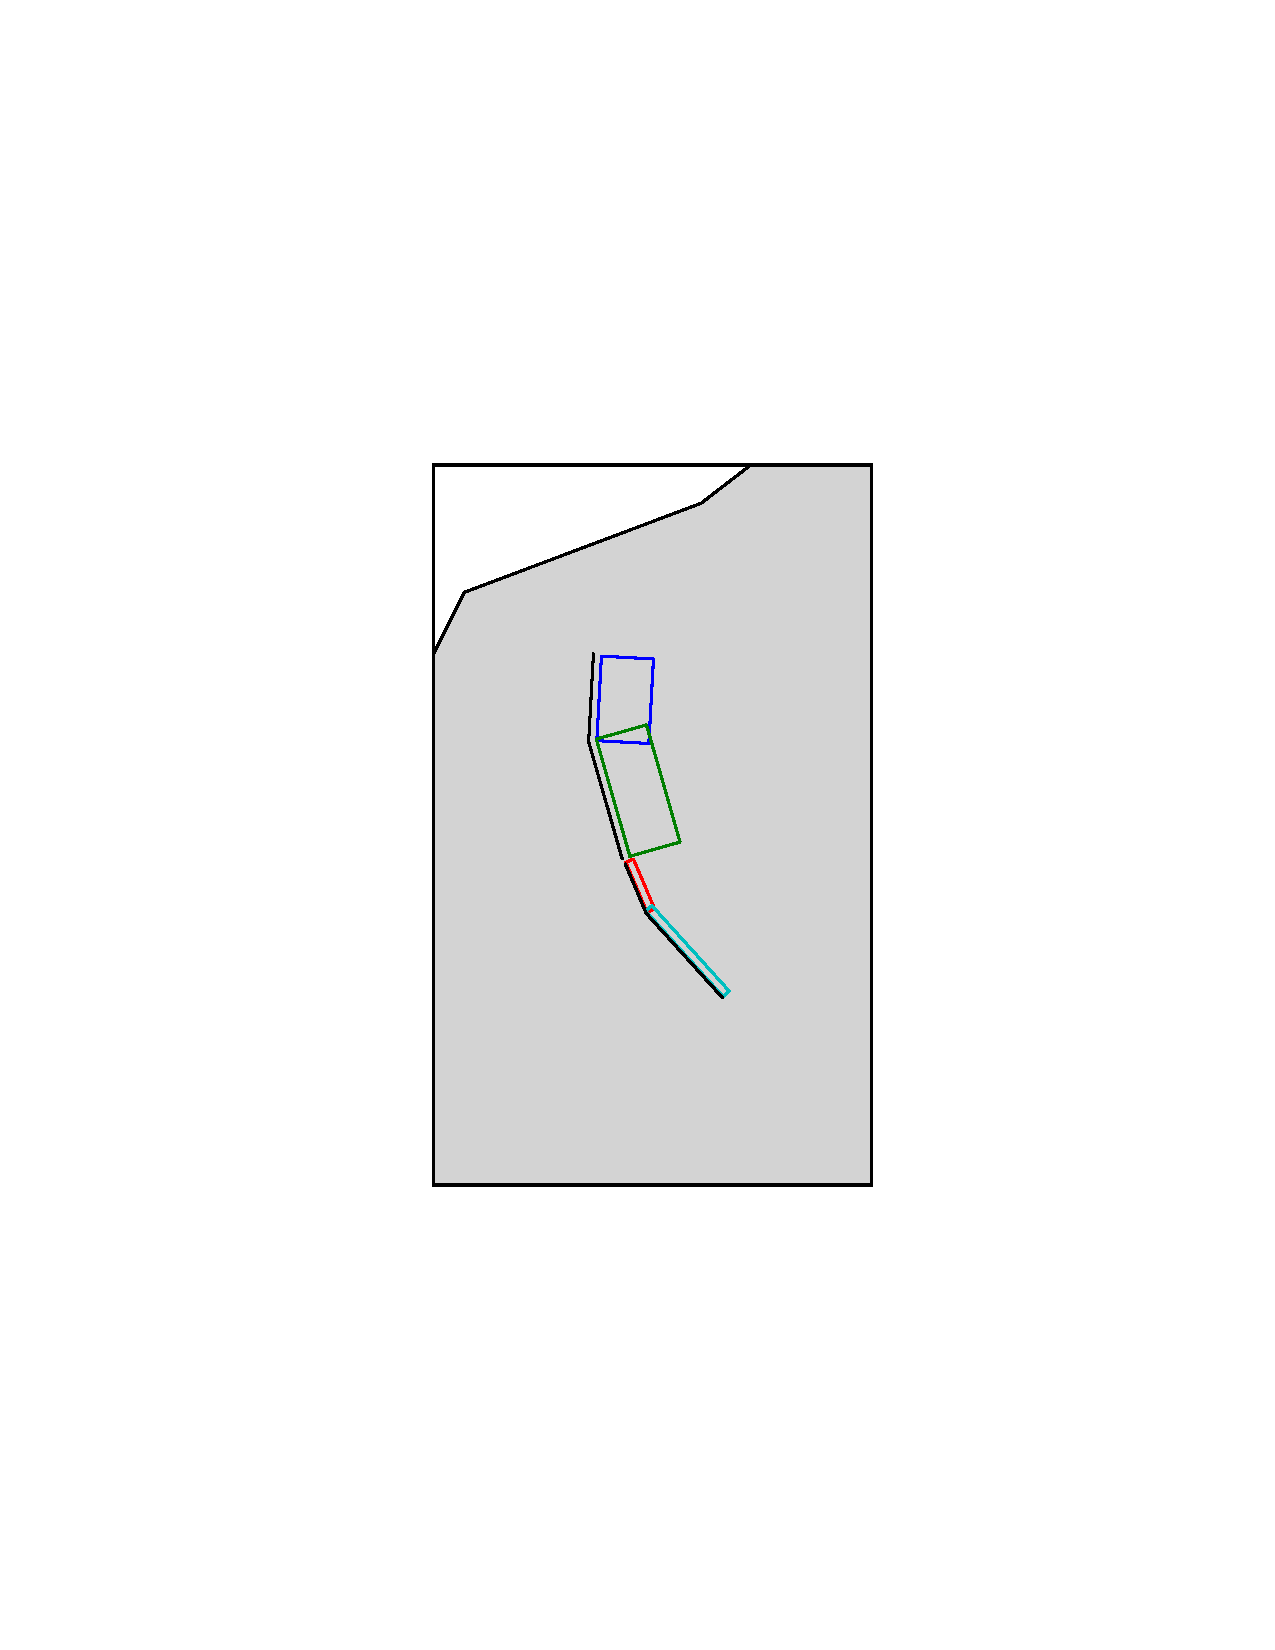
\includegraphics[trim=5cm 7cm 5cm 7cm, clip, width=10cm]{figures/hazard/multi_surface.pdf}
\caption{Geometry of a multi-segmented characteristic fault composed of four
         rectangular ruptures as modelled in OpenQuake.}
\label{fig:char_fault_source}
\end{figure}

\paragraph{Source data}
\begin{itemize}
    \item The characteristic rupture surface is defined through one of the
    following options:
        \begin{itemize}
            \item A list of rectangular ruptures (``planar surfaces'')
            \item A \gls{simplefaultsource} geometry
            \item A \gls{complexfaultsource} geometry
        \end{itemize}
    \item A \gls{frequencymagnitudedistribution}.
    \item Rake angle (specified following the Aki-Richards convention; see
          \citet{aki2002}).
    \item Upper and lower depth values limiting the seismogenic interval.
\end{itemize}

A comprehensive example enumerating the possible rupture surface configurations is shown below. 

\inputminted[firstline=1,firstnumber=1,fontsize=\footnotesize,frame=single,linenos,bgcolor=lightgray]{xml}{oqum/hazard/verbatim/input_characteristic_fault_simple.xml}
\captionof{listing}{Example characteristic fault with simple fault geometry\label{lst:example_characteristic_fault_simple}}

\inputminted[firstline=1,firstnumber=1,fontsize=\footnotesize,frame=single,linenos,bgcolor=lightgray]{xml}{oqum/hazard/verbatim/input_characteristic_fault_complex.xml}
\captionof{listing}{Example characteristic fault with complex fault geometry\label{lst:example_characteristic_fault_complex}}

\inputminted[firstline=1,firstnumber=1,fontsize=\footnotesize,frame=single,linenos,bgcolor=lightgray]{xml}{oqum/hazard/verbatim/input_characteristic_fault_planar.xml}
\captionof{listing}{Example characteristic fault with planar/multi-planar fault geometry\label{lst:example_characteristic_fault_planar}}



%\begin{mdframed}[]
%\inputminted[firstline=1,firstnumber=1,fontsize=%\footnotesize,frame=single,linenos,bgcolor=lightgray]{xml}{oqum/hazard/verbatim/input_nonparametric_source.xml}
%\caption{Example non-parametric source with planar, multi-planar, simple fault %and complex fault geometry}
%\label{lst:example_nonparametric_source}
%\end{mdframed}
%\input{oqum/hazard/verbatim/input_nonparametric_source}



\subsection{Non-Parametric Sources}
\subsubsection{Non-Parametric Fault}
\label{desc_nonparametric_fault}
\index{Source type!fault!nonparametric}
\index{Non-Parametric fault|see{Source type}}

The non-parametric fault typology requires that the user indicates the rupture properties (rupture surface, magnitude, rake and hypocentre) and the corresponding probabilities of the rupture. The probabilities are given as a list of floating point values that correspond to the probabilities of $0, 1, 2, \ldots ... N$ occurrences of the rupture within the specified investigation time. Note that there is not, at present, any internal check to ensure that the investigation time to which the probabilities refer corresponds to that specified in the configuration file. As the surface of the rupture is set explicitly, no rupture floating occurs, and, as in the case of the characteristic fault source, the rupture surface can be defined as either a single planar rupture, a list of planar ruptures, a \gls{simplefaultsource} geometry, a \gls{complexfaultsource} geometry, or a combination of different geometries.

Comprehensive examples enumerating the possible configurations are shown below:

\inputminted[firstline=1,firstnumber=1,fontsize=\footnotesize,frame=single,linenos,bgcolor=lightgray]{xml}{oqum/hazard/verbatim/input_nonparametric_planar.xml}
\captionof{listing}{Example non-parametric fault with planar and multi-planar fault geometry\label{lst:example_nonparametric_planar}}
\inputminted[firstline=1,firstnumber=1,fontsize=\footnotesize,frame=single,linenos,bgcolor=lightgray]{xml}{oqum/hazard/verbatim/input_nonparametric_simple.xml}
\captionof{listing}{Example characteristic fault with simple fault geometry\label{lst:example_nonparametric_simple}}
\inputminted[firstline=1,firstnumber=1,fontsize=\footnotesize,frame=single,linenos,bgcolor=lightgray]{xml}{oqum/hazard/verbatim/input_nonparametric_complex.xml}
\captionof{listing}{Example characteristic fault with complex fault geometry\label{lst:example_nonparametric_complex}}



\section{Magnitude-frequency distributions}
\label{sec:mfd_list}
The magnitude-frequency distributions currently supported by the
\gls{acr:oqe} are the following:

\begin{description}

\item[A discrete incremental magnitude-frequency distribution]
It is the simplest distribution supported. It is defined by the minimum value
of magnitude (representing the mid point of the first bin) and the bin width.
The distribution itself is simply a sequence of floats describing the annual
number of events for different bins. The maximum magnitude admitted by this
magnitude-frequency distribution is just the sum of the minimum magnitude and
the product of the bin width by the number annual rate values. Below we provide an example of the xml that should be incorporated in a
seismic source description in order to define this \gls{acr:mfd}.


\begin{minted}[firstline=1,firstnumber=1,fontsize=\footnotesize,frame=single,bgcolor=lightgray]{xml}
<incrementalMFD minMag="5.05" binWidth="0.1">
    <occurRates>0.15 0.08 0.05 0.03 0.015</occurRates>
</incrementalMFD>
\end{minted}

The magnitude-frequency distribution obtained with the above parameters is
represented in Figure~\ref{fig:evenly_discretized_mfd}.

\begin{figure}[!ht]
\centering
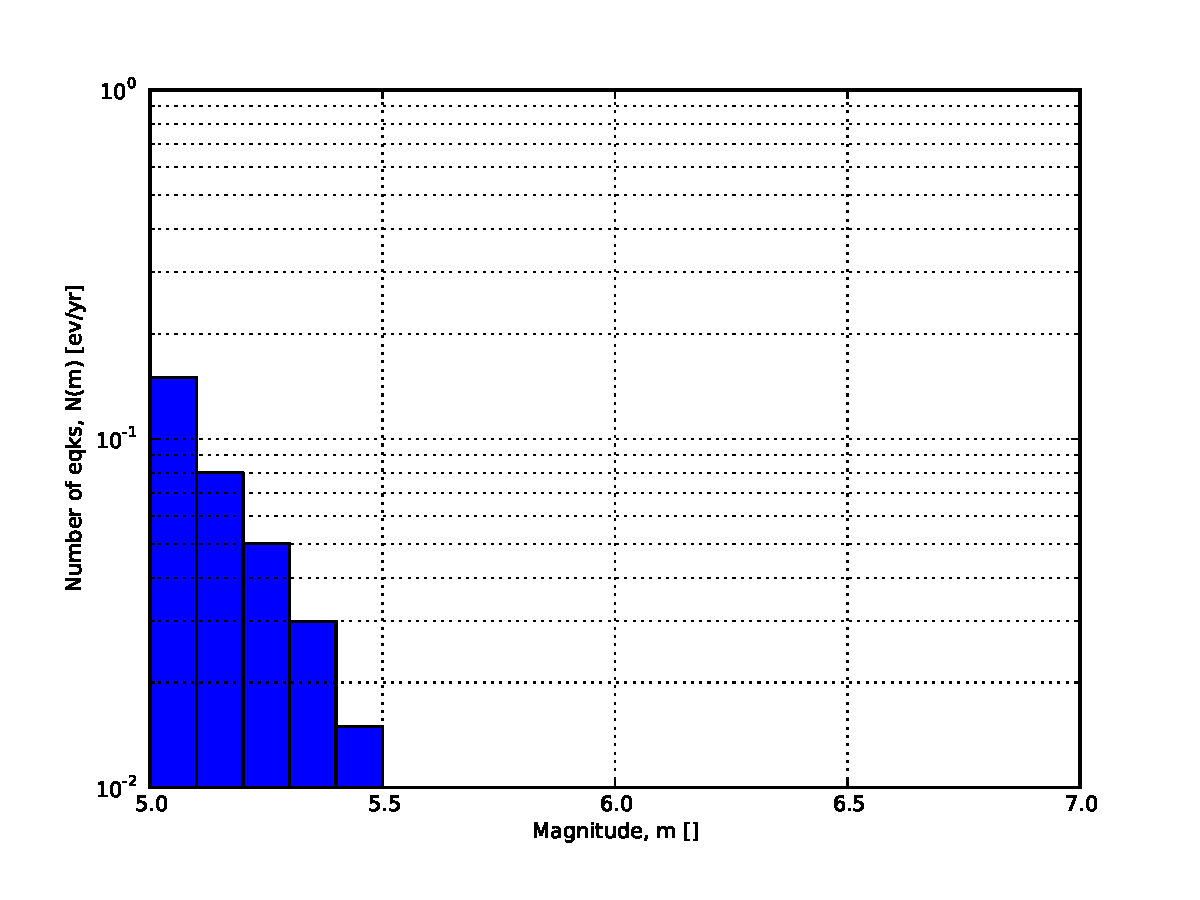
\includegraphics[width=12cm]{figures/hazard/ed_mfd.pdf}
\caption{Example of an incremental magnitude-frequency distribution.}
\label{fig:evenly_discretized_mfd}
\end{figure}

\item[A double truncated Gutenberg-Richter distribution]
This distribution is described by means of a minimum \texttt{minMag} and
maximum magnitude \texttt{maxMag} and by the $a$ and $b$ values of the
Gutenberg-Richter relationship.

The syntax of the xml used to describe this magnitude-frequency distribution
is rather compact as demonstrated in the following example:

\begin{minted}[firstline=1,firstnumber=1,fontsize=\footnotesize,frame=single,bgcolor=lightgray]{xml}
<truncGutenbergRichterMFD aValue="5.0" bValue="1.0" minMag="5.0"
                          maxMag="6.0"/>
\end{minted}

Figure~\ref{fig:dt_gr_mfd} shows the magnitude-frequency distribution
obtained using the parameters of the considered example.

\begin{figure}[!ht]
\centering
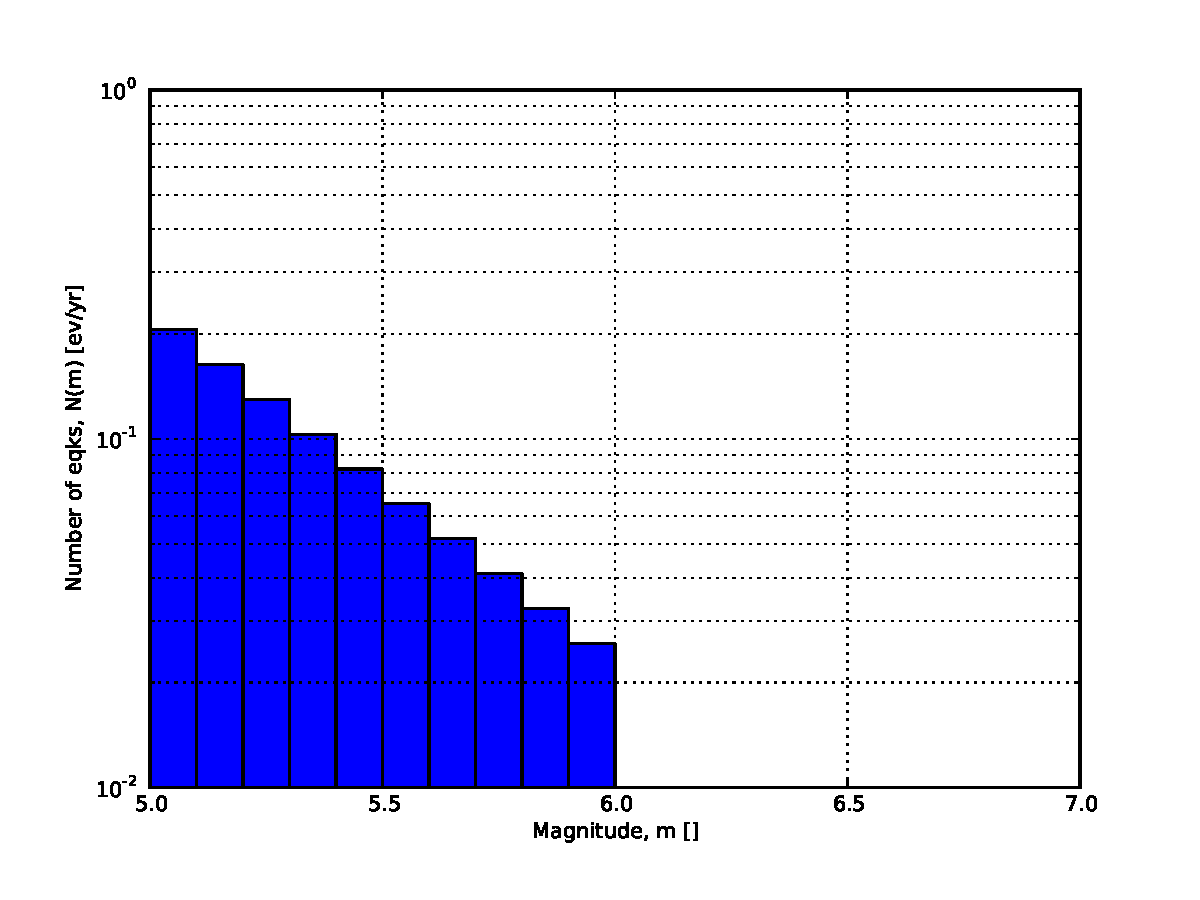
\includegraphics[width=12cm]{figures/hazard/dt_mfd.pdf}
\caption{Example of a double truncated Gutenberg-Richter magnitude-frequency
distribution.}
\label{fig:dt_gr_mfd}
\end{figure}

\item[Hybrid Characteristic earthquake model (\`{a} la \cite{youngs1985})]
The hybrid characteristic earthquake model, presented by \cite{youngs1985},
distributes seismic moment proportionally between a characteristic model (for
larger magnitudes) and an exponential model. The rate of events is dependent
on the magnitude of the characteristic earthquake, the b-value and the total
moment rate of the system (Figure \ref{fig:yc_gr_mfd}). However, the total
moment rate may be defined in one of two ways. If the total moment rate of the
source is known, as may be the case for a fault surface with known area and
slip rate, then the distribution can be defined from the total moment rate (in
N-m) of the source directly. Alternatively, the distribution can be defined
from the rate of earthquakes in the characteristic bin, which may be
preferable if the distribution is determined from observed seismicity
behaviour. The option to define the distribution according to the total moment
rate is input as:


\begin{minted}[firstline=1,firstnumber=1,fontsize=\footnotesize,frame=single,bgcolor=lightgray]{xml}
<YoungsCoppersmithMFD minmag="5.0" bValue="1.0" binWidth="0.1"
                      characteristicMag="7.0" totalMomentRate="1.05E19"/>
\end{minted}


\noindent whereas the option to define the distribution from the rate of
the characteristic events is given as:

\begin{minted}[firstline=1,firstnumber=1,fontsize=\footnotesize,frame=single,bgcolor=lightgray]{xml}
<YoungsCoppersmithMFD minmag="5.0" bValue="1.0" binWidth="0.1"
                      characteristicMag="7.0" characteristicRate="0.005"/>
\end{minted}

Note that in this distribution the width of the magnitude bin must be defined
explicitly in the model.

\begin{figure}[!ht]
\centering
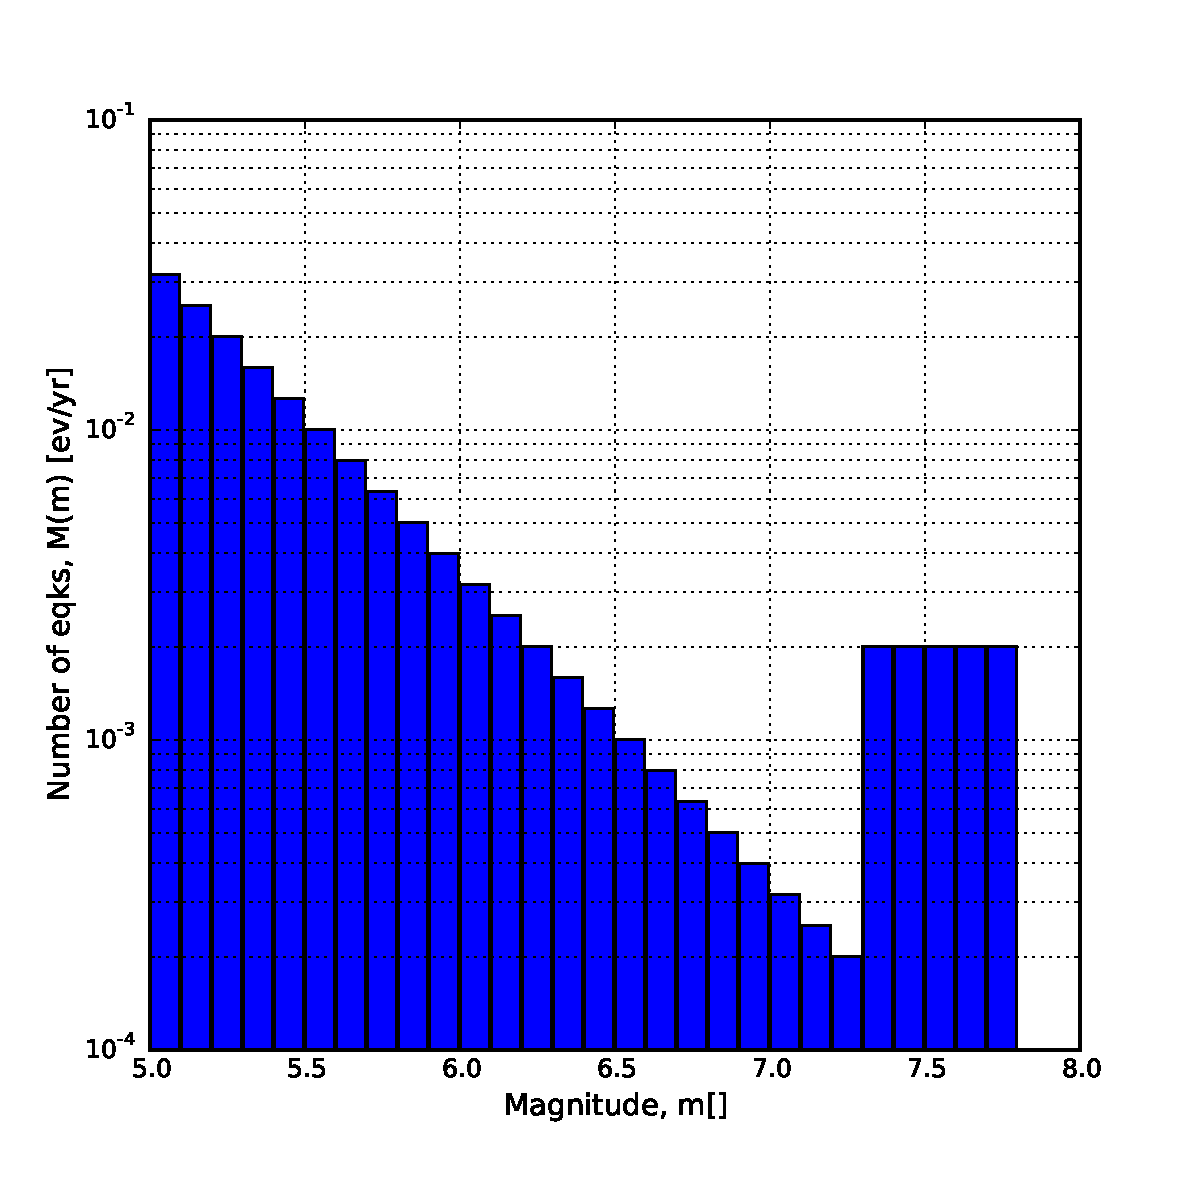
\includegraphics[width=10cm]{figures/hazard/yc_mfd_char_rate.pdf}
\caption{\cite{youngs1985} magnitude-frequency distribution.}
\label{fig:yc_gr_mfd}
\end{figure}

\item[``Arbitrary'' Magnitude Frequency Distribution]
The arbitrary magnitude frequency distribution is another non-parametric form
of MFD, in which the rates are defined explicitly. Here, the magnitude
frequency distribution is defined by a list of magnitudes and their
corresponding rates of occurrence. There is no bin-width as the rates
correspond exactly to the specific magnitude. Unlike the evenly discretised
MFD, there is no requirement that the magnitudes be equally spaced. This
distribution (illustrated in Figure \ref{fig:arb_mfd}) can be input as:

\begin{minted}[firstline=1,firstnumber=1,fontsize=\footnotesize,frame=single,bgcolor=lightgray]{xml}
<arbitraryMFD>
    <occurRates>0.12 0.036 0.067 0.2</occurRates>
    <magnitudes>8.1 8.47 8.68 9.02</magnitude>
</arbitraryMFD>
\end{minted}

\begin{figure}[!ht]
\centering
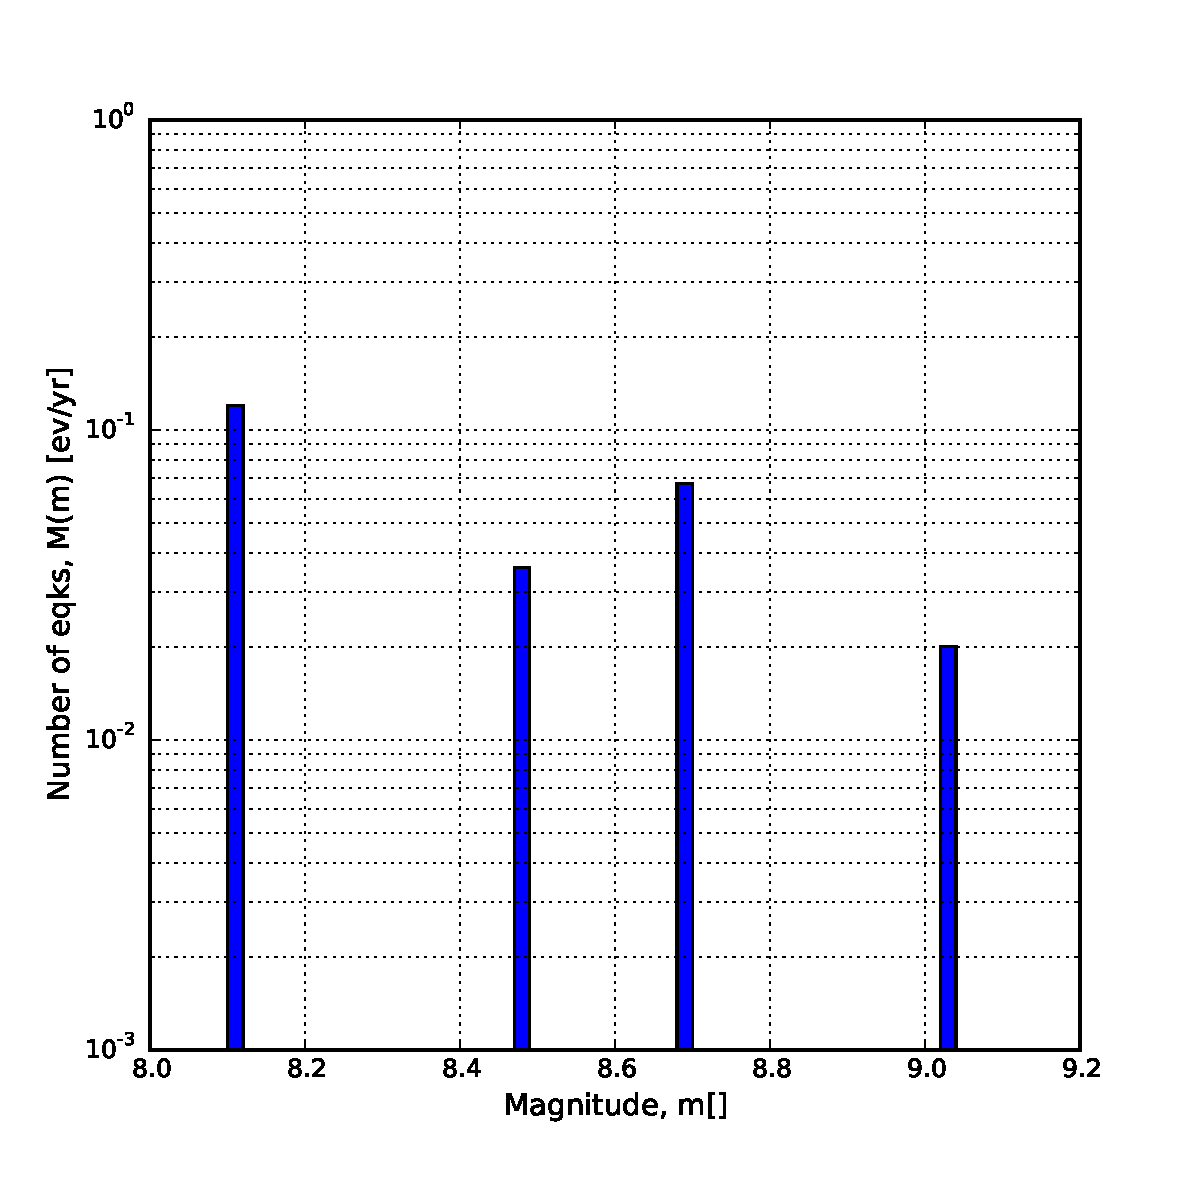
\includegraphics[width=10cm]{figures/hazard/arb_mfd.pdf}
\caption{``Arbitrary'' magnitude-frequency distribution.}
\label{fig:arb_mfd}
\end{figure}

\end{description}

\section{Magnitude-scaling relationships}
\label{sec:msr_list}
We provide below a list of the magnitude-area scaling relationships
implemented in the \gls{acr:hazlib}:

\subsection{Relationships for shallow earthquakes in active tectonic regions}

\begin{itemize}

    \item \cite{wells1994} - One of the most well known magnitude scaling
	relationships, based on a global database of historical earthquake
	ruptures. The implemented relationship is the one linking magnitude to
	rupture area, and is called with the keyword \verb=WC1994=

\end{itemize}


\subsection{Magnitude-scaling relationships for subduction earthquakes}
\begin{itemize}
    \item \cite{Strasser2010} - Defines several magnitude scaling relationships for interface and in-slab earthquakes. Only the magnitude to rupture-area scaling relationships are implemented here, and are called with the keywords \verb=StrasserInterface= and \verb=StrasserIntraslab= respectively.
    \item \cite{Thingbaijam2017} - Define  magnitude scaling relationships for interface. Only the magnitude to rupture-area scaling relationships are implemented here, and are called with the keywords \verb=ThingbaijamInterface=.
\end{itemize}

\subsection{Magnitude-scaling relationships stable continental regions}
\begin{itemize}
    \item \cite{ceus2011} - Defines a single magnitude to rupture-area scaling relationship for use in the central and eastern United States: $Area = 10.0^{M_W - 4.336}$. It is called with the keyword \verb=CEUS2011=
\end{itemize}

\subsection{Miscellaneous Magnitude-Scaling Relationships} 
\begin{itemize}
    \item \verb=PeerMSR= defines a simple magnitude scaling relation used as part of the Pacific Earthquake Engineering Research Center verification of probabilistic seismic hazard analysis programs: $Area = 10.0 ^{M_W - 4.0}$.
    \item \verb=PointMSR= approximates a `point' source by returning an infinitesimally small area for all magnitudes. Should only be used for distributed seismicity sources and not for fault sources. 
\end{itemize}

%
%\subsection{Ground motion prediction equations for volcanic areas}
%\begin{itemize}
%    \item
%\end{itemize}


\section{Calculation workflows}
\index{OpenQuake-engine!Hazard calculation workflows}
\label{sec:hazard_calculators}
The hazard component of the \glsdesc{acr:oqe} can compute seismic hazard using
various approaches. Three types of analysis are currently supported:

\begin{itemize}

	\item \textit{Classical Probabilistic Seismic Hazard Analysis (PSHA)},
	allowing calculation of hazard curves and hazard maps following the
	classical integration procedure (\cite{cornell1968}, \citet{mcguire1976})
	as formulated by \cite{field2003}.

	\item \textit{Event-Based Probabilistic Seismic Hazard Analysis},
	allowing calculation of ground-motion fields from stochastic event sets.
	Traditional results - such as hazard curves - can be obtained by post-
	processing the set of computed ground-motion fields.

	\item \textit{\gls{acr:ssha}}, allowing the calculation of ground
	motion fields from a single earthquake rupture scenario taking into
	account ground-motion aleatory variability.

\end{itemize}

Each workflow has a modular structure, so that intermediate results can be
exported and analyzed. Each calculator can be extended independently of the
others so that additional calculation options and methodologies can be easily
introduced, without affecting the overall calculation workflow.



\subsection{Classical Probabilistic Seismic Hazard Analysis}
\index{OpenQuake-engine!Hazard calculation workflows!Classical PSHA}
\label{subsec:classical_psha}
Input data for the classical \gls{acr:psha} consist of a PSHA input model
provided together with calculation settings.

The main calculators used to perform this analysis are the following:

\begin{enumerate}

	\item \emph{Logic Tree Processor}

	The Logic Tree Processor (LTP) takes as an input the \gls{acr:psha} Input
	Model and creates a Seismic Source Model. The LTP uses the information in
	the Initial Seismic Source Models and the Seismic Source Logic Tree to
	create a Seismic Source Input Model (i.e. a model describing geometry and
	activity rates of each source without any epistemic uncertainty).

	Following a procedure similar to the one just described the Logic Tree
	Processor creates a Ground Motion model (i.e. a data structure that
	associates to each tectonic region considered in the calculation a
	\gls{acr:gmpe}).

	\item \emph{Earthquake Rupture Forecast Calculator}

	The produced Seismic Source Input Model becomes an input information for
	the Earthquake Rupture Forecast (ERF) calculator which creates a list
	earthquake ruptures admitted by the source model, each one characterized
	by a probability of occurrence over a specified time span.

	\item \emph{Classical PSHA Calculator}

	The classical PSHA calculator uses the ERF and the Ground Motion model to
	compute hazard curves on each site specified in the calculation settings.

\end{enumerate}

\subsection{Event-Based Probabilistic Seismic Hazard Analysis}
\index{OpenQuake-engine!Hazard calculation workflows!Event-based PSHA}
\label{subsec:event_based_psha}
Input data for the Event-Based PSHA - as in the case of the Classical
\gls{acr:psha} calculator - consists of a PSHA Input Model and a set of
calculation settings.

The main calculators used to perform this analysis are:

\begin{enumerate}

	\item \emph{Logic Tree Processor}

	The Logic Tree Processor works in the same way described in  the
	description of the Classical \gls{acr:psha} workflow  (see
	Section~\ref{subsec:classical_psha} at
	page~\pageref{subsec:classical_psha}).

	\item \emph{Earthquake Rupture Forecast Calculator}

	The Earthquake Rupture Forecast Calculator was already  introduced in the
	description of the PSHA workflow (see Section~\ref{subsec:classical_psha}
	at page~\pageref{subsec:classical_psha}).

	\item \emph{Stochastic Event Set Calculator}

	The Stochastic Event Set Calculator generates a collection of stochastic
	event sets by sampling the ruptures contained in the ERF according to
	their probability of occurrence.

	A Stochastic Event Set (SES) thus represents a potential realisation of
	the seismicity (i.e. a list of ruptures) produced by the set of seismic
	sources considered in the analysis over the time span fixed for the
	calculation of hazard.

	\item \emph{Ground Motion Field Calculator}

	The Ground Motion Field Calculator computes for each event contained in a
	Stochastic Event Set a realization of the geographic distribution of the
	shaking by taking into account the aleatory uncertainties in the ground-
	motion model. Eventually, the Ground Motion Field calculator can consider
	the spatial correlation of the ground-motion during the generation of the
	\gls{acr:gmf}.

	\item \emph{Event-based PSHA Calculator}

	The event-based PSHA calculator takes a (large) set of ground-motion
	fields representative of the possible shaking scenarios that the
	investigated area can experience over a (long) time span and for each
	site computes the corresponding hazard curve.

	This procedure is computationally intensive and is not recommended for
	investigating the hazard over large areas.

\end{enumerate}

\subsection{Scenario based Seismic Hazard Analysis}
\index{OpenQuake-engine!Hazard calculation workflows!Scenario-based SHA}
\label{subsec:scenario_hazard}
In case of \gls{acr:ssha}, the input data consist of a single earthquake
rupture model and one or more ground-motion models. Using the Ground Motion
Field Calculator, multiple realizations of ground shaking can be computed,
each realization sampling the aleatory uncertainties in the ground-motion
model. The main calculator used to perform this analysis is the \emph{Ground
Motion Field Calculator}, which was already introduced during the description
of the event based PSHA workflow (see Section~\ref{subsec:event_based_psha} at
page~\pageref{subsec:event_based_psha}).

As the scenario calculator does not need to determine the probability of
occurrence of the specific rupture, but only sufficient information to
parameterise the location (as a three-dimensional surface), the magnitude and
the style-of-faulting of the rupture, a more simplified NRML structure is
sufficient compared to the source model structures described previously in
Section~\ref{sec:source_typologies}.
A \emph{rupture model} XML can be defined in the following formats:

\begin{enumerate}

    \item \emph{Simple Fault Rupture} - in which the geometry is defined by the
    trace of the fault rupture, the dip and the upper and lower seismogenic
    depths. An example is shown below in Listing~\ref{lst:input_rupture_simple}.

\begin{listing}[htbp]
  \inputminted[firstline=1,firstnumber=1,fontsize=\footnotesize,frame=single,linenos,bgcolor=lightgray]{xml}{oqum/hazard/verbatim/input_rupture_simple_fault.xml}
  \caption{An example simple fault rupture input file}
  \label{lst:input_rupture_simple}
\end{listing}

    \item \emph{Planar \& Multi-Planar Rupture} - in which the geometry is
    defined as a collection of one or more rectangular planes, each defined
    by four corners. An example of a multi-planar rupture is shown below
    in Listing~\ref{lst:input_rupture_multi_planes}.

\begin{listing}[htbp]
  \inputminted[firstline=1,firstnumber=1,fontsize=\footnotesize,frame=single,linenos,bgcolor=lightgray]{xml}{oqum/hazard/verbatim/input_rupture_multi_planes.xml}
  \caption{An example multi-planar rupture input file}
  \label{lst:input_rupture_multi_planes}
\end{listing}

    \item \emph{Complex Fault Rupture} - in which the geometry is defined by
    the upper, lower and (if applicable) intermediate edges of the fault
    rupture. An example of a complex fault rupture is shown below in
    Listing~\ref{lst:input_rupture_complex}.

\begin{listing}[htbp]
  \inputminted[firstline=1,firstnumber=1,fontsize=\footnotesize,frame=single,linenos,bgcolor=lightgray]{xml}{oqum/hazard/verbatim/input_rupture_complex.xml}
  \caption{An example complex fault rupture input file}
  \label{lst:input_rupture_complex}
\end{listing}

\end{enumerate}


\cleardoublepage
   \cleardoublepage

\chapterimage{figures/chapter_head.pdf} % Chapter heading image
\chapter{Using the Hazard Module}
	\label{chap:hazinputs}
	This Chapter summarises the structure of the information necessary to define
a PSHA input model to be used with the \glsdesc{acr:oqe}.

Input data for probabilistic based seismic hazard analysis (Classical, Event
based, Disaggregation, and UHS) are organised into:

\begin{itemize}

	\item A general configuration file.

    \item A file describing the Seismic Source System, that is the set of
	initial source models and associated epistemic uncertainties needed to
	model the seismic activity in the region of interest.

    \item A file describing the Ground Motion System, that is the set of
	ground motion prediction equations, per tectonic region type, needed to
	model the ground motion shaking in the region of interest.

\end{itemize}

Figure~\ref{fig:psha_input} summarises the structure of a PSHA input model
for the \glsdesc{acr:oqe} and the relationships between the different files.

\begin{figure}[!ht]
\centering
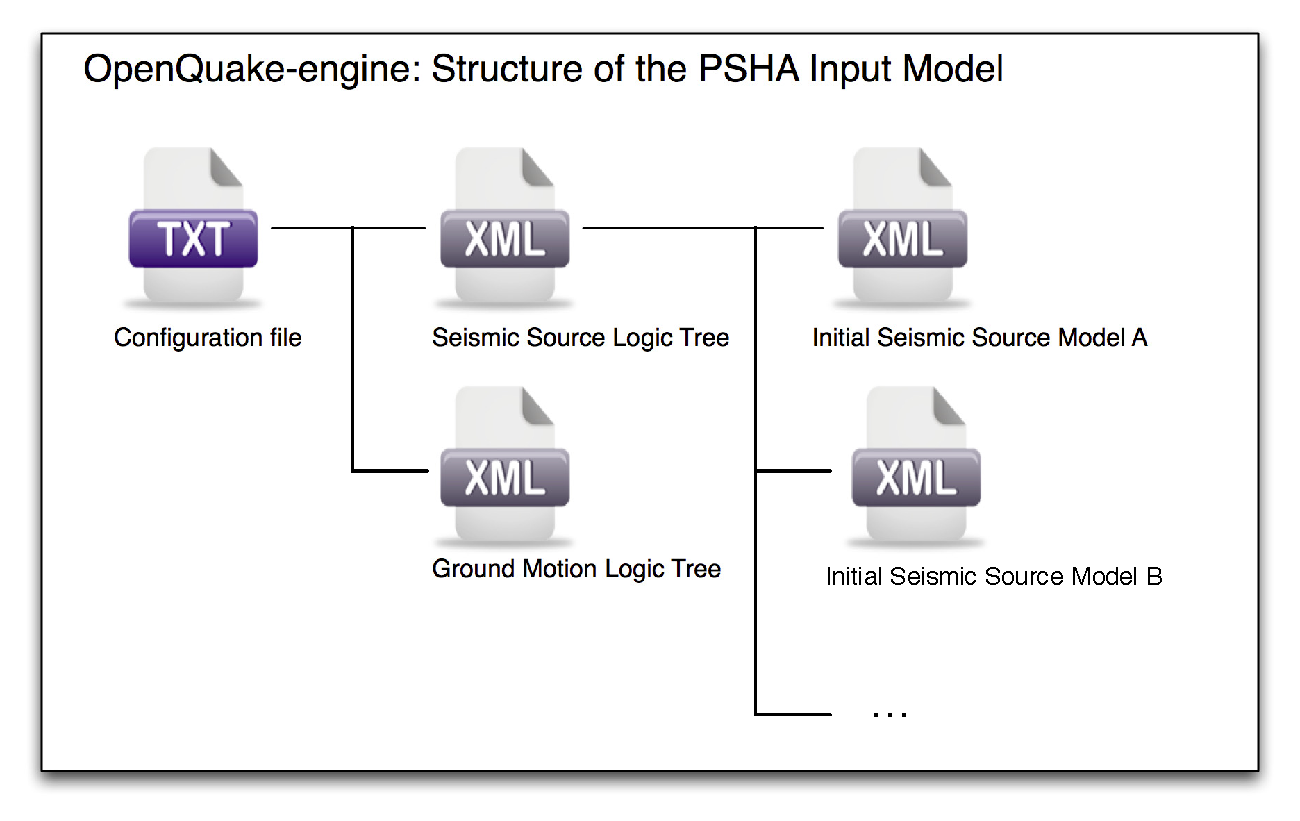
\includegraphics[width=14cm]{figures/hazard/psha_input_structure.pdf}
\caption{PSHA Input Model structure}
\label{fig:psha_input}
\end{figure}


\section{Defining Logic Trees}
The main components of a logic tree structure in the \glsdesc{acr:oqe} are the
following:

\begin{description}

    \item[branch]: the simplest component of a logic tree structure. A branch
	represent a possible interpretation of a value assignment for a specific type
	of uncertainty. It is fully described by the tuple (parameter or model,
	weight).

    \item[branching set]: it is a key component in the logic tree structure
	used by the \gls{acr:oqe}. It groups a set of branches i.e. alternative
	interpretations of a parameter or a model. Each branching set is defined by:

    \begin{itemize}

        \item An ID

        \item An uncertainty type (for a comprehensive list of the types of
		uncertainty currently supported see page~\pageref{list_epistemic_unc})

        \item One or more branches

    \end{itemize}

    This set of uncertainties can be applied to the whole initial  seismic
    source input model or just to a subset of seismic sources. The sum of the
    weights/probabilities assigned to the set  of branches always correspond
    to one.

\end{description}

Below we provide a simple schema illustrating the skeleton of xml file
containing the desciption of a logic tree:

\begin{minted}[firstline=1,firstnumber=1,fontsize=\footnotesize,frame=single,bgcolor=lightgray]{xml}
    <logicTreeBranchSet branchSetID=ID
                        uncertaintyType=TYPE>
        <logicTreeBranch>
            <uncertaintyModel>VALUE</uncertaintyModel>
            <uncertaintyWeight>WEIGHT</uncertaintyWeight>
        </logicTreeBranch>
    </logicTreeBranchSet>
\end{minted}

As it appears from this example, the structure of a logic tree is a set of
nested elements.

A schematic representation of the elemental components of a logic tree
structure is provided in Figure~\ref{glts}.
A branch set identifies a collection of
branches (i.e. individual branches)  whose weights sum to 1.

\begin{figure}[!ht]
\centering
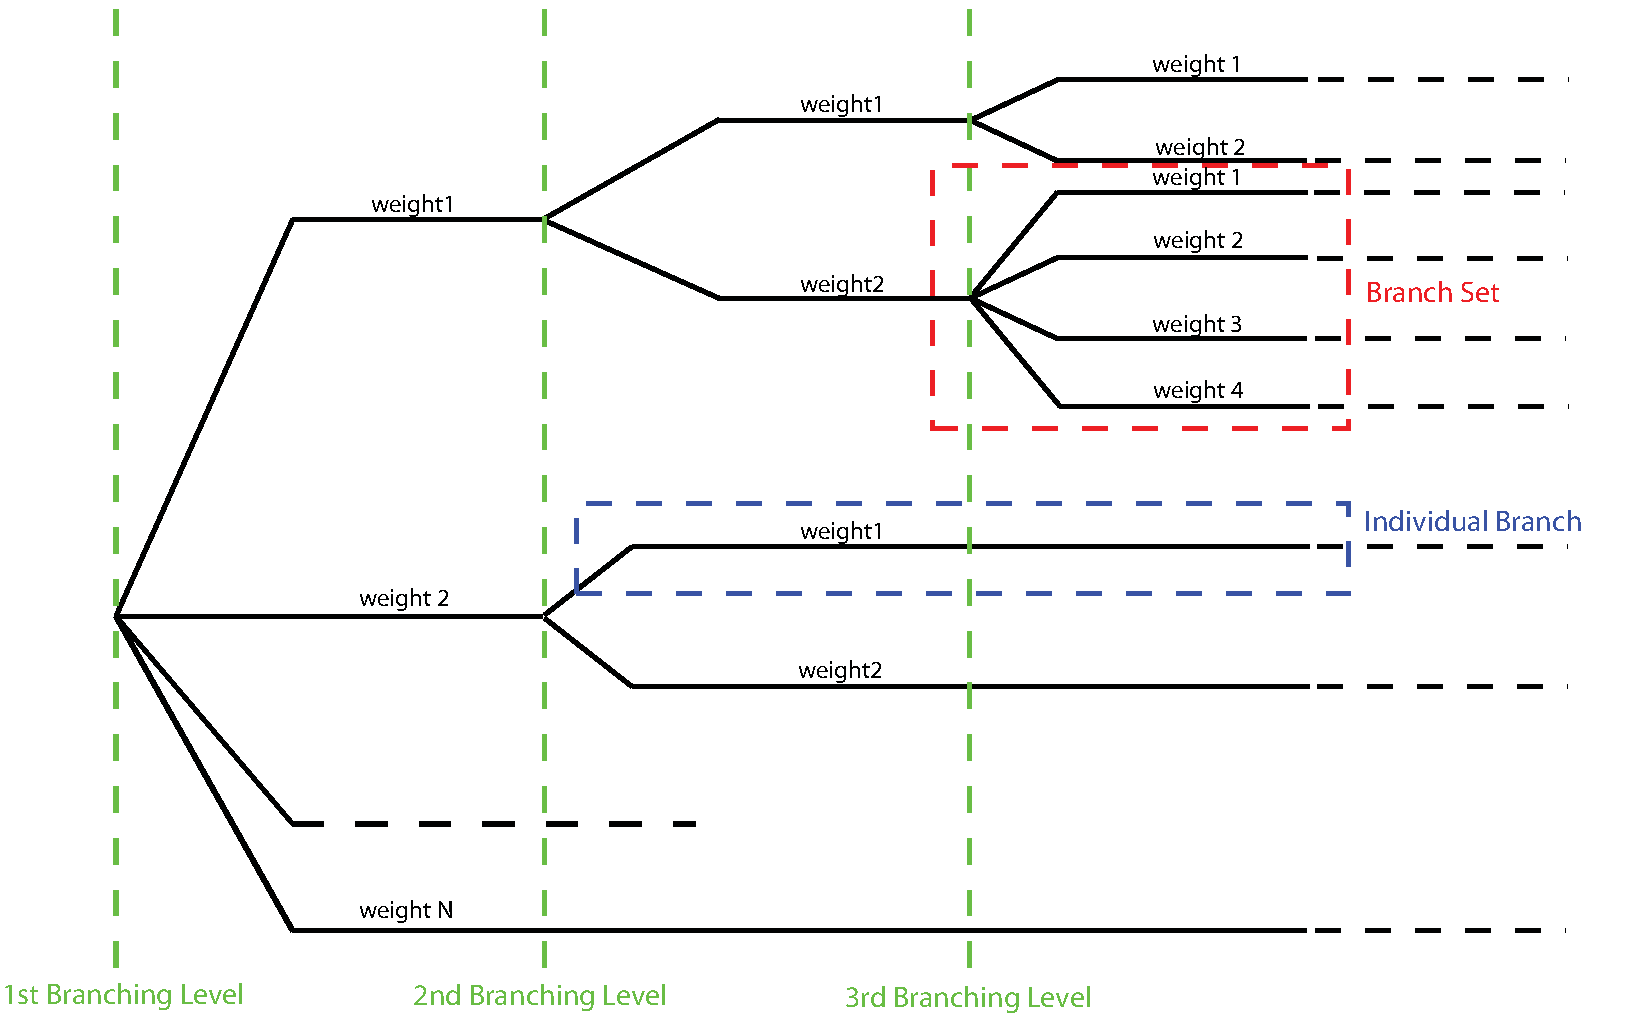
\includegraphics[width=13cm]{figures/hazard/GenericLogicTreeStructure.pdf}
\caption{Generic Logic Tree structure as described in terms of branch sets,
and individual branches.}
\label{glts}
\end{figure}

\subsection{Logic trees as described in the nrml schema}

In the NRML schema, a logic tree structure is defined through the
\Verb+logicTree+ element:

\begin{minted}[firstline=1,firstnumber=1,fontsize=\footnotesize,frame=single,bgcolor=lightgray]{xml}
<logicTree logicTreeID="ID">
...
</logicTree>
\end{minted}

A \Verb+logicTree+ contains as a sequence of \Verb+logicTreeBranchSet+ elements.

There are no restrictions on the number of branch set that can be defined.

Each \Verb+logicTreeBranchSet+
has two required attributes: \Verb+branchSetID+ and
\Verb+uncertaintyType+. The latter defines the type of epistemic uncertainty this branch set is describing.

\begin{minted}[firstline=1,firstnumber=1,fontsize=\footnotesize,frame=single,bgcolor=lightgray]{xml}
<logicTree logicTreeID="ID">
		<logicTreeBranchSet branchSetID="ID_1"
			uncertaintyType="UNCERTAINTY_TYPE">
			...
		</logicTreeBranchSet>
		<logicTreeBranchSet branchSetID="ID_2"
			uncertaintyType="UNCERTAINTY_TYPE">
			...
		</logicTreeBranchSet>
		...
		<logicTreeBranchSet branchSetID="ID_N"
			uncertaintyType="UNCERTAINTY_TYPE">
			...
		</logicTreeBranchSet>
...
</logicTree>
\end{minted}

Possible values for the \Verb+uncertaintyType+ attribute are:

\label{list_epistemic_unc}
\begin{itemize}

    \item \Verb+gmpeModel+: indicates epistemic uncertainties on ground
	motion prediction equations

	\item \Verb+sourceModel+: indicates epistemic uncertainties on source models

    \item \Verb+maxMagGRRelative+: indicates relative (i.e. increments)
	epistemic uncertainties to be added (or subtracted, depending on the sign
	of the increment) to the Gutenberg-Richter maximum magnitude value.

    \item \Verb+bGRRelative+: indicates relative epistemic uncertainties
	to be applied to the Gutenberg-Richter b value.

    \item \Verb+abGRAbsolute+: indicates absolute (i.e. values used to replace
	original values) epistemic uncertainties on the Gutenberg-Richter a and b
	values.

    \item \Verb+maxMagGRAbsolute+: indicates (absolute) epistemic
	uncertainties on the Gutenberg-Richter maximum magnitude.
	
	\item \Verb+incrementalMFDAbsolute+: indicates (absolute) epistemic uncertainties on the incremental magnitude frequency distribution (i.e. alternative rates and/or minimum magnitude) of a specific source (can only be applied to individual sources)
	
	\item \Verb+simpleFaultGeometryAbsolute+: indicates alternative representations of the simple fault geometry for an individual simple fault source
	
	\item \Verb+simpleFaultDipRelative+: indicates a relative increase or decrease in fault dip for one or more simple fault sources
	
	\item \Verb+simpleFaultDipAbsolute+: indicates alternative values of fault dip for one or more simple fault sources
	
	\item \Verb+complexFaultGeometryAbsolute+: indicates alternative representations of complex fault geometry for an individual complex fault source

	\item \Verb+characteristicFaultGeometryAbsolute+: indicates alternative representations of the characteristic fault geometry for an individual characteristic fault source

\end{itemize}

A \Verb+branchSet+ is defined as a sequence of \Verb+logicTreeBranch+
elements, each specified by an \Verb+uncertaintyModel+ element (a string
identifying an uncertainty model; the content of the string varies with the \texttt{uncertaintyType} attribute value of the branchSet element) and the \texttt{uncertaintyWeight} element (specifying the probability/weight associated to the uncertaintyModel):

\begin{minted}[firstline=1,firstnumber=1,fontsize=\footnotesize,frame=single,bgcolor=lightgray]{xml}
< logicTree  logicTreeID="ID">
...

		< logicTreeBranchSet  branchSetID="ID_#"
				uncertaintyType="UNCERTAINTY_TYPE">
			< logicTreeBranch  branchID="ID_1">
				<uncertaintyModel>
				    UNCERTAINTY_MODEL
				</uncertaintyModel>
				<uncertaintyWeight>
				    UNCERTAINTY_WEIGHT
				</uncertaintyWeight>
			</ logicTreeBranch >
			...
			< logicTreeBranch  branchID="ID_N">
				<uncertaintyModel>
				    UNCERTAINTY_MODEL
				</uncertaintyModel>
				<uncertaintyWeight>
				    UNCERTAINTY_WEIGHT
				</uncertaintyWeight>
			</logicTreeBranch>
		</logicTreeBranchSet>
...
</logicTree >
\end{minted}

Depending on the \Verb+uncertaintyType+ the content of the
\Verb+<uncertaintyModel>+ element changes:

\begin{itemize}

    \item if \Verb+uncertaintyType="gmpeModel"+, the uncertainty model
	contains the name of a ground motion prediction equation (a list of
	available GMPEs can be obtained using \texttt{oq info -g} or 
	\texttt{oq info --gsims} and these are also documented at:
	\href{http://docs.openquake.org/oq-engine/2.8/openquake.hazardlib.gsim.html}{http://docs.openquake.org/oq-engine/2.8/openquake.hazardlib.gsim.html}):

    \begin{minted}[firstline=1,firstnumber=1,fontsize=\footnotesize,frame=single,bgcolor=lightgray]{xml}
<uncertaintyModel>GMPE_NAME</uncertaintyModel>
	\end{minted}

    \item if \Verb+uncertaintyType="sourceModel"+, the uncertainty model
	contains the paths to a source model file, e.g.:

    \begin{minted}[firstline=1,firstnumber=1,fontsize=\footnotesize,frame=single,bgcolor=lightgray]{xml}
<uncertaintyModel>SOURCE_MODEL_FILE_PATH</uncertaintyModel>
	\end{minted}

    \item if \Verb+uncertaintyType="maxMagGRRelative"+, the uncertainty model
	contains the increment to be added (or subtracted, depending on the sign)
	to the Gutenberg-Richter maximum magnitude:

    \begin{minted}[firstline=1,firstnumber=1,fontsize=\footnotesize,frame=single,bgcolor=lightgray]{xml}
<uncertaintyModel>MAX_MAGNITUDE_INCREMENT</uncertaintyModel>
	\end{minted}

    \item if \Verb+uncertaintyType="bGRRelative"+, the uncertainty model
	contains the increment to be added (or subtracted, depending on the sign)
	to the Gutenberg-Richter b value:

    \begin{minted}[firstline=1,firstnumber=1,fontsize=\footnotesize,frame=single,bgcolor=lightgray]{xml}
<uncertaintyModel>B_VALUE_INCREMENT</uncertaintyModel>
	\end{minted}

    \item if \Verb+uncertaintyType="abGRAbsolute"+, the uncertainty model
	must contain one a and b pair:

    \begin{minted}[firstline=1,firstnumber=1,fontsize=\footnotesize,frame=single,bgcolor=lightgray]{xml}
<uncertaintyModel>A_VALUE B_VALUE</uncertaintyModel>
	\end{minted}

    \item if \Verb+uncertaintyType="maxMagGRAbsolute"+, the uncertainty
	model must contain one Gutenberg-Richter maximum magnitude value:

    \begin{minted}[firstline=1,firstnumber=1,fontsize=\footnotesize,frame=single,bgcolor=lightgray]{xml}
<uncertaintyModel>MAX_MAGNITUDE</uncertaintyModel>
	\end{minted}
	
	\item if \Verb+uncertaintyType="incrementalMFDAbsolute"+, the uncertainty model must contain an instance of the incremental MFD node:
	
    \begin{minted}[firstline=1,firstnumber=1,fontsize=\footnotesize,frame=single,bgcolor=lightgray]{xml}
<uncertaintyModel>
    <incrementalMFD
        minMag="MIN MAGNITUDE"
        binWidth="BIN WIDTH">
        <occurRates>RATE_1 RATE_2 ... RATE_N</occurRates>
    </incrementalMFD>
</uncertaintyModel>
    \end{minted}

    \item if \Verb+uncertaintyType="simpleFaultGeometryAbsolute"+ then the uncertainty model must contain a \emph{valid} instance of the \verb+simpleFaultGeometry+ node as described in section \ref{desc_simple_fault}

    \item if \Verb+uncertaintyType="simpleFaultDipRelative"+ then the uncertainty model must specify the number of degrees to increase (positive) or decrease (negative) the fault dip. Note that if this increase results in an adjusted fault dip greater than $90^{\circ}$ or less than $0^{\circ}$ an error will occur.
     
    \begin{minted}[firstline=1,firstnumber=1,fontsize=\footnotesize,frame=single,bgcolor=lightgray]{xml}
<uncertaintyModel>DIP_INCREMENT</uncertaintyModel>
	\end{minted}

	\item if \Verb+uncertaintyType="simpleFaultDipAbsolute"+ then the uncertainty model must specify the dip angle (in degrees)

    \begin{minted}[firstline=1,firstnumber=1,fontsize=\footnotesize,frame=single,bgcolor=lightgray]{xml}
<uncertaintyModel>DIP</uncertaintyModel>
	\end{minted}

    \item if \Verb+uncertaintyType="complexFaultGeometryAbsolute"+ then the uncertainty model must contain a \emph{valid} instance of the \verb+complexFaultGeometry+ source node as described in section \ref{desc_complex_fault}
    
    \item if \Verb+uncertaintyType="characteristicFaultGeometryAbsolute"+ then the uncertainty model must contain a \emph{valid} instance of the \verb+characteristicFaultGeometry+ source node, as described in section \ref{desc_characteristic_fault}
\end{itemize}

There are no restrictions on the number of \Verb+logicTreeBranch+ elements
that can be defined in a \Verb+logicTreeBranchSet+, as long as the uncertainty
weights sum to 1.0.

The \Verb+logicTreeBranchSet+ element offers also a number of optional
attributes allowing for complex tree definitions:

\begin{itemize}

    \item \Verb+applyToBranches+: specifies to which \Verb+logicTreeBranch+
	elements (one or more), in the previous branch sets, the branch set
	is linked to. The linking is established by defining the IDs of the
	branches to link to:

	\begin{Verbatim}[commandchars=\\\{\}, samepage=true]
	applyToBranches="branchID1 branchID2 .... branchIDN"
	\end{Verbatim}

    The default is the keyword ALL, which means that a branch set is by
    default linked to all branches in the previous branch set. By
    specifying one or  more branches to which the branch set links to, non-
    symmetric logic trees can be defined.

    \item \Verb+applyToSources+: specifies to which source in a source model
	the uncertainty applies to. Sources are specified in terms of their IDs:

	\begin{Verbatim}[commandchars=\\\{\}, samepage=true]
	applyToSources="srcID1 srcID2 .... srcIDN"
	\end{Verbatim}

    \item \Verb+applyToSourceType+: specifies to which source type the
	uncertainty applies to.  Only one source typology can be defined
	(\Verb+area+, \Verb+point+, \Verb+simpleFault+, \Verb+complexFault+), e.g.:

	\begin{Verbatim}[commandchars=\\\{\}, samepage=true]
	applyToSources="area"
	\end{Verbatim}

    \item \Verb+applyToTectonicRegionType+: specifies to which tectonic
	region type the uncertainty applies to. Only one tectonic region type can
	be defined (\texttt{Active Shallow Crust}, \texttt{Stable
	Shallow Crust}, \texttt{Subduction Interface}, \texttt{Subduction}
	\texttt{IntraSlab}, \texttt{Volcanic}), e.g.:

	\begin{Verbatim}[commandchars=\\\{\}]
	applyToTectonicRegionType="Active Shallow Crust"
	\end{Verbatim}

\end{itemize}
\label{sec:hazard_logic_trees}

\section{The Seismic Source System}
The Seismic Source System contains the model (or the models) describing
position, geometry and activity of seismic sources of engineering importance
for a set of sites as well as the possible epistemic uncertainties to be
incorporated into the calculation of seismic hazard.



\subsection{The Seismic Source Logic Tree}

The structure of the Seismic Source Logic Tree consists of at least one
\gls{branchinglevel}. This branching level is the one used to define the
\gls{initialseismicsourceinputmodel} (or a number of initial seismic source
models, see Figure~\ref{fig:psha_input}).

The example provided below shows the simplest Seismic Source Logic Tree
structure that can be defined in a \gls{pshainputmodel} for \gls{acr:oqe}.
It's a logic tree with just one branching level containing one \gls{branchset}
with one branch used to define the initial seismic source model (its weight
will be equal to one).

\begin{listing}[htbp]
  \inputminted[firstline=1,firstnumber=1,fontsize=\footnotesize,frame=single,linenos,bgcolor=lightgray]{xml}{oqum/hazard/verbatim/input_sslt.xml}
  \caption{Example seismic source model logic tree input file}
  \label{lst:input_sslt}
\end{listing}

The optional branching levels will contain rules that modify parameters of the
sources in the initial seismic source model.

For example, if the epistemic uncertainties to be considered are source
geometry and maximum magnitude, the modeller can create a logic tree structure
with three initial seismic source models (each one exploring a different
definition of the geometry of sources) and one branching level accounting for
the epistemic uncertainty on the maximum magnitude.

Below we provide an example of such logic tree structure. Note that the
uncertainty on the maximum magnitude is specified in terms of relative
increments with respect to the initial maximum magnitude defined for each
source in the initial seismic source models.

\inputminted[firstline=1,firstnumber=1,fontsize=\footnotesize,frame=single,linenos,bgcolor=lightgray]{xml}{oqum/hazard/verbatim/input_sslt_simple_lt.xml}
\captionof{listing}{Example source model logic tree structure\label{lst:example_source_model_logic_tree}}

Starting from \glsdesc{acr:oqe24}, it is also possible to split a source model
into several files and read them as if they were a single file. The file names
for the different files comprising a source model should be provided in the
source model logic tree file. For instance, a source model could be split by
tectonic region using the following syntax in the source model logic tree:

\begin{minted}[firstline=1,firstnumber=1,fontsize=\footnotesize,frame=single,bgcolor=lightgray]{xml}
<?xml version="1.0" encoding="UTF-8"?>
<nrml xmlns:gml="http://www.opengis.net/gml"
      xmlns="http://openquake.org/xmlns/nrml/0.5">
    <logicTree logicTreeID="lt1">
        <logicTreeBranchingLevel branchingLevelID="bl1">
            <logicTreeBranchSet uncertaintyType="sourceModel"
                                branchSetID="bs1">
                <logicTreeBranch branchID="b1">
                    <uncertaintyModel>
		        active_shallow_sources.xml
		        stable_shallow_sources.xml
                    </uncertaintyModel>
                    <uncertaintyWeight>1.0</uncertaintyWeight>
                </logicTreeBranch>
            </logicTreeBranchSet>
        </logicTreeBranchingLevel>
    </logicTree>
</nrml>
\end{minted}


\subsection{The Seismic Source Model}
\index{Input!Configuration file}

The structure of the xml file representing the seismic source model
corresponds to a list of sources, each one modelled using one out of the five
typologies currently supported. Below we provide a schematic example of a
seismic source model:

\begin{listing}[htbp]
  \inputminted[firstline=1,firstnumber=1,fontsize=\footnotesize,frame=single,linenos,bgcolor=lightgray]{xml}{oqum/hazard/verbatim/input_sslt.xml}
  \caption{Example seismic source model input file}
  \label{lst:input_ssm}
\end{listing}
\label{sec:seismic_source_system}

\section{The Ground Motion System}
\index{Input!Ground motion system}
\label{sec:ground_motion_system}
The Ground Motion System defines the models and the possible epistemic
uncertainties related to ground motion modelling to be incorporated into the
calculation.

\subsection{The Ground Motion Logic Tree}
\index{Input!Ground motion logic tree}
\label{subsec:gmlt}

The structure of the \gls{groundmotionlogictree} consists of a list of ground
motion prediction equations for each tectonic region used to characterise the
sources in the PSHA input model.

The example below in Listing~\ref{lst:input_gmlt} shows a simple
\gls{groundmotionlogictree}. This logic tree assumes that all the sources in
the PSHA input model belong to ``Active Shallow Crust'' and uses for
calculation the \citet{chiou2008} \gls{acr:gmpe}.

\begin{listing}[htbp]
  \inputminted[firstline=1,firstnumber=1,fontsize=\footnotesize,frame=single,linenos,bgcolor=lightgray]{xml}{oqum/hazard/verbatim/input_gmlt.xml}
  \caption{Example ground motion logic tree input file}
  \label{lst:input_gmlt}
\end{listing}

\section{Configuration file}
\index{Input!Configuration file!Hazard}
\label{sec:hazard_configuration_file}
The configuration file is the primary file controlling both the definition of
the input model as well as parameters governing the calculation. We illustrate
in the following different examples of the configuration file addressing
different types of seismic hazard calculations.


\subsection[Classical PSHA]{Classical PSHA}
\label{subsec:config_classical_psha}
In the following we describe the overall structure and the most typical
parameters of a configuration file to be used for the computation of a
seismic hazard map using a classical PSHA methodology.


\textbf{Calculation type and model info}

\begin{minted}[firstline=1,linenos=true,firstnumber=1,fontsize=\footnotesize,frame=single,bgcolor=lightgray]{ini}
[general]
description = A demo OpenQuake-engine .ini file for classical PSHA
calculation_mode = classical
random_seed = 1024
\end{minted}

In this section the user specifies the following parameters:

\begin{itemize}

    \item \texttt{description}: a parameter that can be used to designate
    the model

    \item \texttt{calculation\_mode}: it is used to set the kind of
    calculation. In this case it corresponds to \texttt{classical}.
    Alternative options for the calculation\_mode are described later in this
    manual.

    \item \texttt{random\_seed}: is used to control the random generator
    so that when Monte Carlo procedures are used calculations are
    replicable (if the same \texttt{random\_seed} is used you get exactly
    the same results).

\end{itemize}

\textbf{Geometry of the area (or the sites) where hazard is computed}

This section is used to specify where the hazard will be computed. Two
options are available:

The first option is to define a polygon (usually a rectangle) and a distance
(in km) to be used to discretize the  polygon area. The polygon is defined by
a list of longitude-latitude tuples.

An example is provided below:

\begin{minted}[firstline=1,linenos=true,firstnumber=5,fontsize=\footnotesize,frame=single,bgcolor=lightgray]{ini}
[geometry]
region = 10.0 43.0, 12.0 43.0, 12.0 46.0, 10.0 46.0
region_grid_spacing = 10.0
\end{minted}

The second option allows the definition of a number of sites where the hazard
will be computed. Each site is specified in terms of a longitude, latitude tuple.
Optionally, if the user wants to consider the elevation of the sites, a value of
depth [km] can also be specified, where positive values indicate below sea level,
and negative values indicate above sea level (i.e. the topographic surface). If
no value of depth is given for a site, it is assumed to be zero. An example is
provided below:

\begin{minted}[firstline=1,linenos=true,firstnumber=8,fontsize=\footnotesize,frame=single,bgcolor=lightgray]{ini}
[geometry]
sites = 10.0 43.0, 12.0 43.0, 12.0 46.0, 10.0 46.0
\end{minted}

If the list of sites is too long the user can specify the name of a csv file
as shown below:

\begin{minted}[firstline=1,linenos=true,firstnumber=10,fontsize=\footnotesize,frame=single,bgcolor=lightgray]{ini}
[geometry]
sites_csv = <name_of_the_csv_file>
\end{minted}

The format of the csv file containing the list of sites is a sequence of
points (one per row) specified in terms of the longitude, latitude tuple. Depth
values are again optional. An example is provided below:

\begin{minted}[firstline=1,linenos=false,firstnumber=10,fontsize=\footnotesize,frame=single,bgcolor=lightgray]{text}
179.0,90.0
178.0,89.0
177.0,88.0
\end{minted}

\textbf{Logic tree sampling}

The \gls{acr:oqe} provides two options for processing the whole logic tree
structure. The first option uses Montecarlo sampling; the user in this case
specifies a number of realizations.

In the second option all the possible realizations are created. Below we
provide an example for the latter option. In this case we set the
\texttt{number\-\_of\-\_logic\_tree\_samples} to 0. \gls{acr:oqe} will perform
a complete enumeration of all  the possible paths from the roots to the leaves
of the logic tree  structure.

\begin{minted}[firstline=1,linenos=true,firstnumber=12,fontsize=\footnotesize,frame=single,bgcolor=lightgray]{ini}
[logic_tree]
number_of_logic_tree_samples = 0
\end{minted}

If the seismic source logic tree and the ground motion logic tree do not
contain epistemic uncertainties the engine will create a single PSHA input.

\textbf{Generation of the earthquake rupture forecast}

\begin{minted}[firstline=1,linenos=true,firstnumber=14,fontsize=\footnotesize,frame=single,bgcolor=lightgray]{ini}
[erf]
rupture_mesh_spacing = 5
width_of_mfd_bin = 0.1
area_source_discretization = 10
\end{minted}

This section of the configuration file is used to specify the level of
discretization of the mesh representing faults, the grid used to delineate the
area sources and, the magnitude-frequency distribution. Note that the smaller
is the mesh spacing (or the bin width) the larger are (1) the precision in the
calculation and (2) the computation demand.

In cases where the source model may contain a mixture of simple and complex
ruptures it is possible to define a different rupture mesh spacing for complex
faults only. This may be helpful in models that permit floating ruptures over
large subduction sources, in which the nearest source to site distances may be
larger than 20 - 30 km, and for which a small mesh spacing would produce a
very large number of ruptures. The spacing for complex faults only can be
configured by the line:

\begin{minted}[firstline=1,linenos=true,firstnumber=18,fontsize=\footnotesize,frame=single,bgcolor=lightgray]{ini}
complex_rupture_mesh_spacing = 10
\end{minted}

\textbf{Parameters describing site conditions}

\begin{minted}[firstline=1,linenos=true,firstnumber=18,fontsize=\footnotesize,frame=single,bgcolor=lightgray]{ini}
[site_params]
reference_vs30_type = measured
reference_vs30_value = 760.0
reference_depth_to_2pt5km_per_sec = 5.0
reference_depth_to_1pt0km_per_sec = 100.0
\end{minted}

In this section the user specifies local soil conditions. The simplest
solution is to define uniform site conditions (i.e. all the sites have  the
same characteristics).

Alternatively it is possible to define spatially variable soil properties in
a separate file; the engine will then assign to each investigation location
the values of the closest point used to specify site conditions.

\begin{minted}[firstline=1,linenos=true,firstnumber=23,fontsize=\footnotesize,frame=single,bgcolor=lightgray]{ini}
[site_params]
site_model_file = site_model.xml
\end{minted}

The file containing the site model has the following structure:

\begin{listing}[htbp]
  \inputminted[firstline=1,firstnumber=1,fontsize=\footnotesize,frame=single,linenos,bgcolor=lightgray]{xml}{oqum/hazard/verbatim/input_site_model.xml}
  \caption{Example site model input file}
  \label{lst:input_site_model}
\end{listing}
\begin{minted}[firstline=1,linenos=false,firstnumber=1,fontsize=\footnotesize,frame=single,bgcolor=lightgray]{xml}

\end{minted}

If the closest available site with soil conditions is at a distance greater than 5~km from the investigation location, a warning is generated.

\textbf{Calculation configuration}
\phantomsection
\label{sec:calculation_configuration}

\begin{minted}[firstline=1,linenos=true,firstnumber=25,fontsize=\footnotesize,frame=single,bgcolor=lightgray]{ini}
[calculation]
source_model_logic_tree_file = source_model_logic_tree.xml
gsim_logic_tree_file = gmpe_logic_tree.xml
investigation_time = 50.0
intensity_measure_types_and_levels = {"PGA": [0.005, ..., 2.13]}
truncation_level = 3
maximum_distance = 200.0
\end{minted}

This section of the \gls{acr:oqe} configuration file specifies the parameters
that are relevant for the calculation of hazard. These include the names of
the two files containing the Seismic Source System and the Ground Motion
System, the duration of the time window used to compute the  hazard, the
ground motion intensity measure types and levels for  which the probability of
exceedence will be computed, the level of truncation of the Gaussian
distribution of the logarithm of ground motion used in the calculation of
hazard and the maximum integration distance (i.e. the distance within which
sources will contribute to the computation of the hazard).

The maximum distance refers to the largest distance between a rupture and the
target calculation sites in order for the rupture to be considered in the PSHA
calculation. This can be input directly in terms of kilometres (as above).
There may be cases, however, in which it may be appropriate to have a
different maximum source to site distance depending on the tectonic region
type. This may be used, for example, to eliminate the impact of small, very
far-field sources with very low activity rates in stable tectonic regions (in
which case maximum distance is reduced), or conversely it may be raised to
allow certain source types to contribute to the hazard at greater distances
(such as in the case of large subduction interface events). An example
configuration for a maximum distance in Active Shallow Crust of 200 km, and in
Stable Continental Crust of 150 km, is shown below:

\begin{minted}[firstline=1,linenos=true,firstnumber=31,fontsize=\footnotesize,frame=single,bgcolor=lightgray]{ini}
maximum_distance = {'Stable Continental Crust': 150.0,
                    'Active Shallow Crust': 200.0}
\end{minted}

An even more advanced approach is to use a maximum distance depending on the
magnitude (magnitude-distance filter): in that case the user must specify
the maximum distance per a discrete set of magnitudes. Here is an
example:

\begin{minted}[fontsize=\footnotesize,frame=single,bgcolor=lightgray]{ini}
maximum_distance = {'Stable Continental Crust': [(8, 250), (7, 150), (5, 50)],
                    'Active Shallow Crust': [(8, 300), (7, 200), (5, 100)]}
\end{minted}

You should read this example as follows: for Stable Continental Crust

\begin{itemize}
\item keep sites within 250 km from the rupture if the magnitude is <= 8
\item keep sites within 150 km from the rupture if the magnitude is <= 7
\item keep sites within 50 km from the rupture if the magnitude is <= 5
\end{itemize}

while for Active Shallow Crust

\begin{itemize}
\item keep sites within 300 km from the rupture if the magnitude is <= 8
\item keep sites within 200 km from the rupture if the magnitude is <= 7
\item keep sites within 100 km from the rupture if the magnitude is <= 5
\end{itemize}

It is also possible to define something like the following:

\begin{minted}[fontsize=\footnotesize,frame=single,bgcolor=lightgray]{ini}
maximum_distance = [(8, 250), (7, 150), (5, 50)]
\end{minted}

In this case the same magnitude-distance filter is used for all tectonic
region types.

If the magnitude is above the maximum magnitude of the filter
(in this example 8) we keep the sites within 2000 km of the ruptures, i.e.
effectively we do not filter.

Notice that the filtering has a big impact on the performance, by
reducing the maximum distance for small magnitudes one can easily
speed up the calculations by 2-3 times or more, without losing much
precision.

\textbf{Output}

\begin{minted}[firstline=1,linenos=true,firstnumber=31,fontsize=\footnotesize,frame=single,bgcolor=lightgray]{ini}
[output]
export_dir = outputs/
# given the specified `intensity_measure_types_and_levels`
mean_hazard_curves = true
quantile_hazard_curves = 0.1 0.5 0.9
uniform_hazard_spectra = false

poes = 0.1
\end{minted}

The final section of the configuration file is the one that contains the
parameters controlling the types of output to be produced. Providing an export
directory will tell OpenQuake where to place the output files when the
\texttt{-{}-exports} flag is used when running the program. Setting
\verb=mean_hazard_curves= to true will result in a specific output containing
the mean curves of the logic tree, likewise \verb=quantile_hazard_curves= will
produce separate files containing the quantile hazard curves at the quantiles
listed (0.1, 0.5 and 0.9 in the example above, leave blank or omit if no
quantiles are required). Setting \verb=uniform_hazard_spectra= to true will
output the uniform hazard spectra at the same probabilities of exceedence
(poes) as those specified by the later option \verb=poes=. The probabilities
specified here correspond to the set investigation time.

By default, OpenQuake will export only the statistical results, i.e. mean
curves and quantiles. If the user requires the complete results for all
realizations, there is a specific command for that, `oq extract hazard/all`.
Beware that if the logic tree contains a large number of end branches the
process of exporting the results from each end branch can add a significant
amount of time - possibly longer than the computation time - and result in a
large volume of disk spaced being used. In this case it is best to postprocess
the data programmatically. Please contact us and we will be happy to give
directions on how to do that in Python.


\subsection{Seismic hazard disaggregation}
\label{subsec:config_hazard_disaggregation}
In this section we describe the structure of the configuration file to be used
to complete a seismic hazard disaggregation. Since only a few parts of the
standard configuration file need to be changed we can use the description
given in Section~\ref{subsec:config_classical_psha} at
page~\pageref{subsec:config_classical_psha} as a reference and we emphasize
herein major differences.

\begin{minted}[firstline=1,linenos=true,firstnumber=1,fontsize=\footnotesize,frame=single,bgcolor=lightgray]{ini}
[general]
description = A demo .ini file for PSHA disaggregation
calculation_mode = disaggregation
random_seed = 1024
\end{minted}

The calculation mode parameter in this case is set as
\texttt{disaggregation}.

\textbf{Geometry of the area (or the sites) where hazard is computed}

\begin{minted}[firstline=1,linenos=true,firstnumber=5,fontsize=\footnotesize,frame=single,bgcolor=lightgray]{ini}
[geometry]
sites = 11.0 44.5
\end{minted}

In the section it is necessary to specify the geographic coordinates of
the site(s) where the disaggregation will be performed. The coordinates
of multiple site should be separated with a comma.

\textbf{Disaggregation parameters}

The disaggregation parameters need to be added to the the standard
configuration file. They are shown in the following example and a description
of each parameter is provided below.

\begin{minted}[firstline=1,linenos=true,firstnumber=7,fontsize=\footnotesize,frame=single,bgcolor=lightgray]{ini}
[disaggregation]
poes_disagg = 0.02, 0.1
mag_bin_width = 1.0
distance_bin_width = 25.0
coordinate_bin_width = 1.5
num_epsilon_bins = 3
disagg_outputs = Mag_Dist_Eps Mag_Lon_Lat
num_rlzs_disagg = 3
rlz_index = 22,23
\end{minted}

\begin{itemize}

    \item \Verb+poes_disagg+: disaggregation is performed for the intensity
    measure levels corresponding to the probability of exceedance value(s) provided
    here. The computations use the \texttt{investigation\_time} and the
    \texttt{intensity\_measure\_types\_and\_levels} defined in the
    ``Calculation configuration'' section   (see page~\pageref{sec:calculation_configuration}).
    For the \texttt{poes\_disagg} the intensity measure level(s) for the disaggregation are
    inferred by performing a classical calculation and by inverting the hazard curves.

    \item \Verb+iml_disagg+: the intensity measure level(s) to be disaggregated
	    can be directly defined by specifying \texttt{iml\_disagg}. Note
		that a disaggregation computation requires either
		\texttt{poes\_disagg} or \texttt{iml\_disagg} to be defined, but
		both cannot be defined at the same time.

    \item \Verb+mag_bin_width+: mandatory; specifies the width of every
	    magnitude histogram bin of the disaggregation matrix computed

    \item \Verb+distance_bin_width+: specifies the width of every distance
	    histogram bin of the disaggregation matrix computed (km)

    \item \Verb+coordinate_bin_width+: specifies the width of every
	    longitude-latitude histogram bin of the disaggregation matrix
		computed (decimal degrees)

    \item \Verb+num_epsilon_bins+: mandatory; specifies the number of epsilon
	    histogram bins of the disaggregation matrix. The width of the
		epsilon bins depends on the \texttt{truncation\_level} defined
		in the ``Calculation configuration'' section
		(page~\pageref{sec:calculation_configuration})

    \item \Verb+disagg_outputs+: optional; specifies the type(s) of
	    disaggregation to be computed. The options are: \texttt{Mag},
		\texttt{Dist}, \texttt{Lon\_Lat}, \texttt{Lon\_Lat\_TRT},
		\texttt{Mag\_Dist}, \texttt{Mag\_Dist\_Eps},
		\texttt{Mag\_Lon\_Lat}, \texttt{TRT}. If none are specified,
		then all are computed. More details of the disaggregation output
		are given in the ``Outputs from Hazard Disaggregation'' section,
		see page~\pageref{subsec:output_hazard_disaggregation})

    \item \Verb+disagg_by_src+: optional; if specified and set to true,
	    disaggregation by source is computed. This option currently only
		works if the logic tree is trivial (i.e. there is only one
		realization).

    \item \Verb+num_rlzs_disagg+: optional; specifies the number of realizations
	    to be used, selecting those that yield intensity measure levels
		closest to the mean.  

    \item \Verb+rlz_index+: optional; specifies the index or indices of
	    the realization/s to disaggregate as a list of comma-separated
		integers.

\end{itemize}

If \texttt{num\_rlzs\_disagg} is specified, the user should not specify
\texttt{rlz\_index}, and vice versa. If neither is specified, the
realization that yields the intensity measure level closest to the mean will be
selected. The mean disaggregation is based on only the selected realizations,
$not$ all the realizations of the model.  

As mentioned above, the user also has the option to perform disaggregation by
directly specifying the intensity measure level to be disaggregated, rather than
specifying the probability of exceedance. An example is shown below:

\begin{minted}[firstline=1,linenos=true,firstnumber=7,fontsize=\footnotesize,frame=single,bgcolor=lightgray]{ini}
[disaggregation] iml_disagg = {'PGA': 0.1} \end{minted}

If \texttt{iml\_disagg} is specified, the user should not include
\texttt{intensity\_measure\_types\_and\_levels} in the ``Calculation
configuration'' section (see page~\pageref{sec:calculation_configuration}) since
it is explicitly given here.


\subsection{Event based PSHA}
\label{subsec:config_event_based_psha}
In the following we describe the sections of the configuration file that are
required to complete event based PSHA calculations


\textbf{Calculation type and model info}

This part is almost identical to the corresponding one described in
Section~\ref{subsec:config_classical_psha}. Note the setting of the
\texttt{calculation\_mode} parameter which now corresponds to
\texttt{event\_based}.

\begin{minted}[firstline=1,linenos=true,firstnumber=1,fontsize=\footnotesize,frame=single,bgcolor=lightgray]{ini}
[general]
description = A demo OpenQuake-engine .ini file for event based PSHA
calculation_mode = event_based
random_seed = 1024
\end{minted}

\textbf{Event based parameters}

This section is used to specify the number of stochastic event sets to be
generated for each logic tree realisation (each stochastic event set
represents a potential realisation of seismicity during the
\texttt{investigation\_time} specified in the
\texttt{calculation\_configuration} part). Additionally, in this section the
user can specify the spatial correlation model to be used for the generation
of ground motion fields.

\begin{minted}[firstline=1,linenos=false,firstnumber=1,fontsize=\footnotesize,frame=single,bgcolor=lightgray]{ini}
ses_per_logic_tree_path = 5
ground_motion_correlation_model = JB2009
ground_motion_correlation_params = {"vs30_clustering": True}
\end{minted}

The acceptable flags for the parameter \verb+vs30_clustering+ are \verb+False+
and \verb+True+, with a capital \verb+F+ and \verb+T+ respectively. \verb+0+
and \verb+1+ are also acceptable flags.

\textbf{Output}

This part substitutes the \texttt{Output} part described in  the configuration
file example described in the Section~ \ref{subsec:config_classical_psha} at
page~\pageref{subsec:config_classical_psha}.

\begin{minted}[firstline=1,linenos=false,firstnumber=1,fontsize=\footnotesize,frame=single,bgcolor=lightgray]{ini}
[output]
export_dir = /tmp/xxx
save_ruptures = true
ground_motion_fields = true
# post-process ground motion fields into hazard curves,
# given the specified `intensity_measure_types_and_levels`
hazard_curves_from_gmfs = true
mean_hazard_curves = true
quantile_hazard_curves = 0.15 0.5 0.85
poes = 0.1 0.2
\end{minted}

Starting from \glsdesc{acr:oqe22}, it is now possible to export information
about the ruptures directly in CSV format.

The option \verb=hazard_curves_from_gmfs= instructs the user to use the event-
based ground motion values to provide hazard curves indicating the
probabilities of exceeding the intensity measure levels set previously in the
\verb=intensity_measure_types_and_levels= option.


\subsection{Scenario hazard}
\label{subsec:config_scenario_hazard}
In order to run this calculator, the parameter \Verb+calculation_mode+ needs
to be set to \Verb+scenario+. The basic job configuration file required for
running a scenario hazard calculation is shown in
Listing~\ref{lst:config_scenario_hazard}.

\begin{listing}[htbp]
  \inputminted[firstline=1,firstnumber=1,fontsize=\footnotesize,frame=single,linenos,bgcolor=lightgray,label=job.ini]{ini}{oqum/hazard/verbatim/config_scenario.ini}
  \caption{Example configuration file for a scenario hazard calculation (\href{https://raw.githubusercontent.com/gem/oq-engine/master/oqum/hazard/verbatim/config_scenario.ini}{Download example})}
  \label{lst:config_scenario_hazard}
\end{listing}

Most of the job configuration parameters required for running a scenario
hazard calculation seen in the example in
Listing~\ref{lst:config_scenario_hazard} are the same as those described in
the previous sections for the classical PSHA calculator
(Section~\ref{subsec:config_classical_psha}) and the event-based PSHA
calculator (Section~\ref{subsec:config_event_based_psha}). The set of sites at
which the ground motion fields will be produced can be specifed by using
either the \Verb+sites+ or \Verb+sites_csv+ parameters, or the \Verb+region+
and \Verb+region_grid_spacing+  parameters, similar to the classical PSHA and
event-based PSHA calculators. The parameter unique to the scenario calculator
is described below:

\begin{itemize}

  \item \Verb+number_of_ground_motion_fields+: this parameter is used to
    specify the number of Monte Carlo simulations of the ground motion
    values at the specified sites

  \item \Verb+gsim+: this parameter indicates the name of a ground motion
  prediction equation (a list of available GMPEs can be obtained using
  \texttt{oq info -g} or \texttt{oq info -{}-gsims} and these are also
  documented at: \href{http://docs.openquake.org/oq-engine/2.8/openquake.hazardlib.gsim.html}{http://docs.openquake.org/oq-engine/2.8/openquake.hazardlib.gsim.html})

\end{itemize}

Multiple ground motion prediction equations can be used for a scenario hazard
calculation by providing a GMPE logic tree file (described previously in 
Section~\ref{subsec:gmlt}) using the parameter \Verb+gsim_logic_tree_file+.
In this case, the \glsdesc{acr:oqe} generates ground motion fields
for all GMPEs specified in the logic tree file. The branch weights in the logic
tree file are ignored in a scenario analysis and only the individual branch
results are computed. Mean or quantile ground motion fields will not be 
generated.

The ground motion fields will be computed at each of the sites and for each of
the intensity measure types specified in the job configuration file. The
above calculation can be run using the command line:

\begin{minted}[fontsize=\footnotesize,frame=single,bgcolor=lightgray]{shell-session}
user@ubuntu:~\$ oq engine --run job.ini
\end{minted}

After the calculation is completed, a message similar to the following will be
displayed:

\begin{minted}[fontsize=\footnotesize,frame=single,bgcolor=lightgray]{shell-session}
Calculation 260 completed in 3 seconds. Results:
  id | name
 569 | gmf_data
\end{minted}

   \cleardoublepage

\chapterimage{figures/chapter_head.pdf} % Chapter heading image
\chapter{Hazard Calculations and Results}
	\label{chap:hazoutputs}
	In this Chapter we provide a desciption of the main commands available for
running hazard with the \gls{acr:oqe} and the file formats used to represent
the results of the analyses.

A general introduction on the use of the \glsdesc{acr:oqe} is provided in
Chapter~\ref{chap:intro} at page~\pageref{chap:intro}. The
reader is invited to consult this part before diving into the following
sections.


% -----------------------------------------------------------------------------
\section{Running OpenQuake-engine for hazard calculations}
\label{sec:running_hazard_calculations}
\index{Running OpenQuake!hazard}

The execution of a hazard analysis using the OpenQuake-engine is
straightforward. Below we provide an example of the simplest command that can be
used to launch a hazard calculation. It consists in the invocation of \texttt
{oq engine} together with the \texttt{-{}-run} option,
and the name of a configuration file (in the example below it
corresponds to \texttt{job.ini}):

\begin{minted}[firstline=1,linenos=false,firstnumber=1,fontsize=\footnotesize,frame=single,bgcolor=lightgray]{bash}
user@ubuntu:$ oq engine --run job.ini
\end{minted}

The amount of information prompted during the execution of the analysis can be
controlled through the \texttt{-{}-log-level} flag as shown in the example below:

\begin{minted}[firstline=1,linenos=false,firstnumber=1,fontsize=\footnotesize,frame=single,bgcolor=lightgray]{bash}
user@ubuntu:$ oq engine --run job.ini --log-level debug
\end{minted}

In this example we ask the engine to provide an extensive amount of information
(usually not justified for a standard analysis). Alternative options are:
\texttt{debug}, \texttt{info}, \texttt{warn}, \texttt{error},
\texttt{critical}.


% -----------------------------------------------------------------------------
\section{Exporting results from a hazard calculation}
\label{sec:exporting_hazard_results}

There are two alternative ways to get results from the OpenQuake-engine:
directly through the calculation or by exporting them from the internal
\gls{acr:oqe} database once a calculation is completed.

The first option is defined at the OpenQuake-engine invocation through the flag \texttt{--exports xml}, as shown in the example below:

\begin{minted}[firstline=1,linenos=false,firstnumber=1,fontsize=\footnotesize,frame=single,bgcolor=lightgray]{bash}
user@ubuntu:~$ oq engine --run job.ini --exports xml
\end{minted}

This will export the results to the \verb=results= directory specified in the \verb=job.ini= file. 

The second option allows the user to export the computed results or just a subset of them whenever they want. In order to obtain the list of results of the hazard calculations stored in the \gls{acr:oqe} database the user can utilize the \texttt{-{}-lhc} command (`list hazard calculations') to list the hazard calculations:

\begin{minted}[firstline=1,linenos=false,firstnumber=1,fontsize=\footnotesize,frame=single,bgcolor=lightgray]{bash}
user@ubuntu:~$ oq engine --lhc
\end{minted}

The execution of this command will produce a list similar to the one provided
below (the numbers in red are the calculations IDs):

\begin{Verbatim}[frame=single, commandchars=\\\{\}, fontsize=\small]
user@ubuntu:~$ oq engine --lhc
job_id | status | start_time | description
\textcolor{red}{1} | failed | 2013-03-01 09:49:34 | Classical PSHA
\textcolor{red}{2} | successful | 2013-03-01 09:49:56 | Classical PSHA
\textcolor{red}{3} | failed | 2013-03-01 10:24:04 | Classical PSHA
\textcolor{red}{4} | failed | 2013-03-01 10:28:16 | Classical PSHA
\textcolor{red}{5} | failed | 2013-03-01 10:30:04 | Classical PSHA
\textcolor{red}{6} | successful | 2013-03-01 10:31:53 | Classical PSHA
\textcolor{red}{7} | failed | 2013-03-09 08:15:14 | Classical PSHA
\textcolor{red}{8} | successful | 2013-03-09 08:18:04 | Classical PSHA
\end{Verbatim}

Subsequently the user can get the list of result stored for a specific hazard
analysis by using the \texttt{-{}-list-outputs}, or \texttt{-{}-lo}, command, as in the example below (note that the number in blue emphasizes the
result ID):

\begin{Verbatim}[frame=single, commandchars=\\\{\}, fontsize=\small]
user@ubuntu:~$ oq engine --lo <calc_id>
id | name
\textcolor{blue}{3} | hcurves
\end{Verbatim}

and finally extract an xml file for a specific hazard result:

\begin{Verbatim}[frame=single, commandchars=\\\{\}, fontsize=\small]
user@ubuntu:~$ oq engine --export-outputs <result_id> <output_folder>
\end{Verbatim}


% -----------------------------------------------------------------------------
\section{Description of hazard outputs}
\label{sec:hazard_outputs}

The results generated by the OpenQuake-engine are fundamentally of two
distinct typologies differentiated by the presence (or absence) of epistemic
uncertainty in the PSHA input model.

When epistemic uncertainty is incorporated into the calculation, the
OpenQuake-engine calculators (e.g. Classical PSHA, Event Based PSHA,
Disaggregation, UHS) produce a set of results (i.e. hazard curves, ground
motion fields, disaggregation matrices, UHS, for each logic-tree realisation)
which reflects epistemic uncertainties introduced in the PSHA input model.
For each logic tree sample, results are computed and stored. Calculation of
results statistics (mean, standard deviation, quantiles) are supported by all
the calculators.

By default, OpenQuake will export only the statistical results, i.e. mean
curves and quantiles. If the user requires the complete results for all
realizations, there is a flag to specify, please see the FAQ \href{https://github.com/gem/oq-engine/blob/engine-3.10/doc/faq-hazard.md}{https://github.com/gem/oq-engine/blob/engine-3.10/doc/faq-hazard.md}.
Beware that if the logic tree contains a large number of end branches the
process of exporting the results from each end branch can add a significant
amount of time - possibly longer than the computation time - and result in a
large volume of disk spaced being used. In this case it is best to postprocess
the data programmatically. Please contact us and we will be happy to give
directions on how to do that in Python.

NB: in the literature there are different algorithms for the computation
of the quantiles. The OpenQuake engine uses an algorithm based on interpolation
which is implemented here:

\href{https://github.com/gem/oq-engine/tree/master/openquake/hazardlib/stats.py}{https://github.com/gem/oq-engine/tree/master/openquake/hazardlib/stats.py}

In particular, the median is computed as the q=0.5 quantile.

\subsection{Outputs from Classical PSHA}
\label{subsec:output_classical_psha}
By default, the classical PSHA calculator computes and stores hazard curves
for each logic tree sample considered.

When the PSHA input model doesn't contain epistemic uncertainties the results
is a set of hazard curves (one for each investigated site). The command below
illustrates how is possible to retrieve the group of hazard curves obtained
for a calculation with a given identifier \texttt{<calc\_id>} (see
Section~\ref{sec:exporting_hazard_results} for an explanation about how to
obtain the list of calculations performed with their corresponding ID):

\begin{Verbatim}[frame=single, commandchars=\\\{\}, fontsize=\small]
user@ubuntu:~$ oq engine --lo <calc_id>
id | name
\textcolor{red}{3 | Hazard Curves}
\textcolor{black}{4 | Realizations}
\end{Verbatim}

To export from the database the outputs (in this case hazard curves) contained
in one of the output identifies, one can do so with the following command:

\begin{Verbatim}[frame=single, commandchars=\\\{\}, fontsize=\small]
user@ubuntu:~$ oq engine --export-output <output_id> <output_directory>
\end{Verbatim}

Alternatively, if the user wishes to export all of the outputs associated with
a particular calculation then they can use the \texttt{-{}-export-outputs}
with the corresponding calculation key:

\begin{Verbatim}[frame=single, commandchars=\\\{\}, fontsize=\small]
user@ubuntu:~$ oq engine --export-outputs <calc_id> <output_directory>
\end{Verbatim}

The exports will produce one or more nrml files containing the seismic hazard
curves, as represented below in Listing~\ref{lst:output_hazard_curves_xml}.

\begin{listing}[htbp]
  \inputminted[firstline=1,firstnumber=1,fontsize=\footnotesize,frame=single,linenos,bgcolor=lightgray]{xml}{oqum/hazard/verbatim/output_hazard_curves.xml}
  \caption{Example hazard curves NRML output file}
  \label{lst:output_hazard_curves_xml}
\end{listing}

Notwithstanding the intuitiveness of this file, let's have a brief overview of
the information included. The overall content of this file is a list of hazard
curves, one for each investigated site, computed using a PSHA input model
representing one possible realisation obtained using the complete logic tree
structure.

The attributes of the \texttt{hazardCurves} element (see text in red) specify
the path of the logic tree used to create the seismic source model
(\texttt{source\-Model\-TreePath}) and the ground motion model
(\texttt{gsim\-Tree\-Path}) plus the intensity measure type and the
investigation time used to compute the probability of exceedance.

The \texttt{IMLs} element (in green in the example) contains the values of
shaking used by the engine to compute the probability of exceedance in the
investigation time. For each site this file contains a \texttt{hazardCurve}
element which has the coordinates (longitude and latitude in decimal degrees)
of the site and the values of the probability of exceedance for all the
intensity measure levels specified in the \texttt{IMLs} element.

If the hazard calculation is configured to produce results including seismic
hazard maps and uniform hazard spectra, then the list of outputs would display
the following:

\begin{Verbatim}[frame=single, commandchars=\\\{\}, fontsize=\small]
user@ubuntu:~$ oq engine --lo <calc_id>
id | name
\textcolor{red}{3 | Hazard Curves}
\textcolor{red}{4 | Hazard Maps}
\textcolor{black}{5 | Realizations}
\textcolor{red}{6 | Uniform Hazard Spectra}
\end{Verbatim}

Listing~\ref{lst:output_hazard_map_xml}) shows a sample of the nrml file
used to describe a hazard map, and and Listing~\ref{lst:output_uhs})
shows a sample of the nrml used to describe a uniform hazard spectrum.

\begin{listing}[htbp]
  \inputminted[firstline=1,firstnumber=1,fontsize=\footnotesize,frame=single,linenos,bgcolor=lightgray]{xml}{oqum/hazard/verbatim/output_hazard_map.xml}
  \caption{Example hazard map NRML output file}
  \label{lst:output_hazard_map_xml}
\end{listing}


\begin{listing}[htbp]
  \inputminted[firstline=1,firstnumber=1,fontsize=\footnotesize,frame=single,linenos,bgcolor=lightgray]{xml}{oqum/hazard/verbatim/output_uhs.xml}
  \caption{Example uniform hazard spectrum NRML output file}
  \label{lst:output_uhs}
\end{listing}

\subsection{Outputs from Hazard Disaggregation}
\label{subsec:output_hazard_disaggregation}
The \glsdesc{acr:oqe} output of a disaggregation analysis corresponds to the
combination of a hazard curve and a multidimensional matrix containing the
results of the disaggregation.

\begin{Verbatim}[frame=single, commandchars=\\\{\}, fontsize=\small]
user@ubuntu:~$ oq engine --lo <calc_id>
id | name
\textcolor{red}{3 | Disaggregation Outputs}
\textcolor{black}{4 | Realizations}
\end{Verbatim}
%\begin{Verbatim}[frame=single, commandchars=\\\{\}]
user@ubuntu:~$ oq engine --lo <calc_id>
id | output_type | name
19 | hazard_curve | hc-rlz-3
20 | hazard_curve | hc-rlz-3
21 | hazard_curve | hc-rlz-4
22 | hazard_curve | hc-rlz-4
23 | disagg_matrix | disagg(0.02)-rlz-3-SA(0.025)-POINT(10.1 40.1)
24 | disagg_matrix | disagg(0.1)-rlz-3-SA(0.025)-POINT(10.1 40.1)
25 | disagg_matrix | disagg(0.02)-rlz-3-PGA-POINT(10.1 40.1)
26 | disagg_matrix | disagg(0.1)-rlz-3-PGA-POINT(10.1 40.1)
27 | disagg_matrix | disagg(0.02)-rlz-4-SA(0.025)-POINT(10.1 40.1)
28 | disagg_matrix | disagg(0.1)-rlz-4-SA(0.025)-POINT(10.1 40.1)
29 | disagg_matrix | disagg(0.02)-rlz-4-PGA-POINT(10.1 40.1)
30 | disagg_matrix | disagg(0.1)-rlz-4-PGA-POINT(10.1 40.1)
\end{Verbatim}

Running \texttt{-{}-export-output} to export the disaggregation results will
produce individual files for each IMT, probability of exceedence and logic tree
realisation. In Listing~\ref{lst:output_disagg_matrix}) we show an example of
the nrml file used to represent the different disaggregation matrices (highlighted
in red) produced by\gls{acr:oqe}:

\begin{listing}[htbp]
  \begin{Verbatim}[frame=single, commandchars=\\\{\}, fontsize=\small]
<?xml version="2.0" encoding="UTF-8"?>
<nrml xmlns:gml="http://www.opengis.net/gml"
      xmlns="http://openquake.org/xmlns/nrml/0.5">
  <disaggMatrices sourceModelTreePath="b1" gsimTreePath="b1" IMT="PGA"
        investigationTime="50.0" lon="10.1" lat="40.1"
        magBinEdges="5.0, 6.0, 7.0, 8.0"
        distBinEdges="0.0, 25.0, 50.0, 75.0, 100.0"
        lonBinEdges="9.0, 10.5, 12.0"
        latBinEdges="39.0, 40.5"
        pdfBinEdges="-3.0, -1.0, 1.0, 3.0"
        tectonicRegionTypes="Active Shallow Crust">
\textcolor{red}{    <disaggMatrix type="Mag" dims="3" poE="0.1" }
\textcolor{red}{            iml="0.033424622602">}
      <prob index="0" value="0.987374744394"/>
      <prob index="1" value="0.704295394366"/>
      <prob index="2" value="0.0802318409498"/>
\textcolor{red}{    </disaggMatrix>}
\textcolor{red}{    <disaggMatrix type="Dist" dims="4" poE="0.1" }
\textcolor{red}{            iml="0.033424622602">}
      <prob index="0" value="0.700851969171"/>
      <prob index="1" value="0.936680387051"/>
      <prob index="2" value="0.761883595568"/>
      <prob index="3" value="0.238687565571"/>
\textcolor{red}{    </disaggMatrix>}
\textcolor{red}{    <disaggMatrix type="TRT" dims="1" poE="0.1" }
\textcolor{red}{            iml="0.033424622602">}
      <prob index="0" value="0.996566187011"/>
\textcolor{red}{    </disaggMatrix>}
\textcolor{red}{    <disaggMatrix type="Mag,Dist" dims="3,4" poE="0.1" }
\textcolor{red}{            iml="0.033424622602">}
      <prob index="2,3" value="0.0"/>
\textcolor{red}{    </disaggMatrix>}
\textcolor{red}{    <disaggMatrix type="Mag,Dist,pdf" dims="3,4,3" poE="0.1" }
\textcolor{red}{            iml="0.033424622602">}
      <prob index="0,0,0" value="0.0785857271425"/>
      ...
\textcolor{red}{    </disaggMatrix>}
\textcolor{red}{    <disaggMatrix type="Lon,Lat" dims="2,1" poE="0.1"}
\textcolor{red}{            iml="0.033424622602">}
      <prob index="0,0" value="0.996566187011"/>
      <prob index="1,0" value="0.0"/>
\textcolor{red}{    </disaggMatrix>}
\textcolor{red}{    <disaggMatrix type="Mag,Lon,Lat" dims="3,2,1" poE="0.1"}
\textcolor{red}{            iml="0.033424622602">}
      <prob index="0,0,0" value="0.987374744394"/>
      <prob index="0,1,0" value="0.0"/>
      <prob index="1,0,0" value="0.704295394366"/>
      <prob index="1,1,0" value="0.0"/>
      <prob index="2,0,0" value="0.0802318409498"/>
      <prob index="2,1,0" value="0.0"/>
\textcolor{red}{    </disaggMatrix>}
\textcolor{red}{    <disaggMatrix type="Lon,Lat,TRT" dims="2,1,1" poE="0.1"}
\textcolor{red}{            iml="0.033424622602">}
      <prob index="0,0,0" value="0.996566187011"/>
      <prob index="1,0,0" value="0.0"/>
\textcolor{red}{    </disaggMatrix>}
  </disaggMatrices>
</nrml>
\end{Verbatim}
  \caption{Example of different disaggregation matrices produced by oq-engine}
  \label{lst:output_disagg_matrix}
\end{listing}




\subsection{Outputs from Event Based PSHA}
\label{subsec:output_event_based_psha}
The Event Based PSHA calculator computes and stores stochastic event sets and
the corresponding ground motion fields.

This calculator can also produce hazard curves and hazard maps exactly in the
same way as done using the Classical PSHA calculator.

The inset below shows an example of the list of results provided by the
\gls{acr:oqe} at the end of an event-based PSHA calculation:

\begin{Verbatim}[frame=single, commandchars=\\\{\}, fontsize=\small]
user@ubuntu:~$ oq engine --lo <calc_id>
id | name
\textcolor{red}{10 | Ground Motion Fields}
11 | Hazard Curves
12 | Hazard Maps
13 | Realizations
\textcolor{blue}{14 | Earthquake Ruptures}
15 | Events
16 | Uniform Hazard Spectra
\end{Verbatim}


This list in the inset above contains a set of ruptures (in green)
and their corresponding sets of ground motion fields (in red).

Exporting the outputs from the ruptures will produce, for each
realisation, a NRML file containing a collection of ruptures.
Below is an example:

\begin{Verbatim}[frame=single, commandchars=\\\{\}, fontsize=\small]
<?xml version="1.0" encoding="UTF-8"?>
<nrml xmlns:gml="http://www.opengis.net/gml"
	  xmlns="http://openquake.org/xmlns/nrml/0.5">
  <stochasticEventSetCollection sourceModelTreePath="b1">
    \textcolor{red}{<stochasticEventSet id="12" investigationTime="50.0">}
\textcolor{green}{     <rupture id="col=00~ses=0001~rup=0049-00"}
\textcolor{green}{         magnitude="4.55" strike="90.0" dip="90.0"}
\textcolor{green}{         rake="90.0" tectonicRegion="Active Shallow Crust">}
\textcolor{green}{       <planarSurface>}
\textcolor{green}{         <topLeft lon="12.233903801" lat="43.256198599"}
\textcolor{green}{                  depth="11.3933265259"/>}
\textcolor{green}{         <topRight lon="12.263958243" lat="43.2562025344"}
\textcolor{green}{                  depth="11.3933265259"/>}
\textcolor{green}{         <bottomLeft lon="12.233903801" lat="43.256198599"}
\textcolor{green}{                  depth="12.6066734741"/>}
\textcolor{green}{         <bottomRight lon="12.263958243" lat="43.2562025344"}
\textcolor{green}{                  depth="12.6066734741"/>}
\textcolor{green}{       </planarSurface>}
\textcolor{green}{     </rupture>}
      <rupture id="col=00~ses=0001~rup=0121-00"
              magnitude="4.65" strike="135.0" dip="90.0"
              rake="90.0" tectonicRegion="Active Shallow Crust">
        <planarSurface>
          <topLeft lon="11.45858812" lat="42.7429056814"
                  depth="11.3208667302"/>
          <topRight lon="11.4822820715" lat="42.7256333907"
                  depth="11.3208667302"/>
          <bottomLeft lon="11.45858812" lat="42.7429056814"
                  depth="12.6791332698"/>
          <bottomRight lon="11.4822820715" lat="42.7256333907"
                  depth="12.6791332698"/>
        </planarSurface>
      </rupture>
    \textcolor{red}{</stochasticEventSet>}
  </stochasticEventSetCollection>
</nrml>
\end{Verbatim}


The text in red shows the part which describes the generated
stochastic event sets and the investigation time covered. Inside the
<SES> tag there is a list of integers (a single integer in this example)
which are unique IDs for the seismic events associated to the rupture.
In general a rupture can occur more than once and the number of events
is given by the multiplicity attribute (in this case 1).

The text in green emphasises the portion of the text used to describe a
rupture. The information provided describes entirely the geometry of the
rupture as well as its rupturing properties (e.g. rake, magnitude). The
rupture ID is an integer that represents each rupture uniquely: it should
not be confused with the event ID, because the multiplicity of a rupture
can be different than 1.

Exporting the outputs from the gmfs will produce an xml file for each
realisation containing the corresponding ground motion fields. Below is an
example of a gmf collection nrml file containing one ground motion field:

\begin{Verbatim}[frame=single, commandchars=\\\{\}, fontsize=\small]
<?xml version="1.0" encoding="UTF-8"?>
<nrml xmlns:gml="http://www.opengis.net/gml"
      xmlns="http://openquake.org/xmlns/nrml/0.5">
  <gmfCollection sourceModelTreePath="b1" gsimTreePath="b1">
    <gmfSet investigationTime="50.0" stochasticEventSetId="12">
      <gmf IMT="PGA" ruptureId="col=00~ses=0001~rup=0049-00">
        <node gmv="0.0105891230432" lon="11.1240023202"
            lat="43.5107462335"/>
        <node gmv="0.00905803920023" lon="11.1241875202"
            lat="43.6006783941"/>
        <node gmv="0.00637664420977" lon="11.1243735810"
            lat="43.6906105547"/>
        <node gmv="0.00476533134789" lon="11.1245605075"
            lat="43.7805427153"/>
        <node gmv="0.00452594698469" lon="11.1247483046"
            lat="43.8704748759"/>
        ...
        <node gmv="0.00017301076646" lon="11.3782630185"
            lat="44.5129482397"/>
      </gmf>
    </gmfSet>
  </gmfCollection>
</nrml>
\end{Verbatim}


The `sourcegroups` output produces a csv file listing the tectonic region
types involved in the calculation and the effective number of ruptures
generated by each of them. An example of such a file is shown below.

\begin{table}[htbp]
\centering
\begin{tabular}{llr}

\hline
\rowcolor{lightgray}
\bf{grp_id} & \bf{trt} & \bf{eff_ruptures} \\
\hline
0 & Active Shallow Crust & 283 \\
1 & Stable Shallow Crust & 24 \\
2 & Subduction Interface & 2 \\
\hline

\end{tabular}
\caption{Example of a source groups output file}
\label{output:event_based_sourcegroups}
\end{table}


\subsection{Outputs from Scenario Hazard Analysis}
\label{subsec:output_scenario_hazard}
By default, the scenario hazard calculator computes and stores
\glspl{acr:gmf} for each GMPE specified in the job configuration file. The
\glspl{acr:gmf} will be computed at each of the sites and for each of the
intensity measure types specified in the job configuration file.

Exporting the outputs from the \glspl{acr:gmf} in the xml format will produce
an xml file for each realisation containing the corresponding ground motion
fields. Listing~\ref{lst:output_gmf_scenario_xml} is an example of a \gls{acr:gmf}
collection NRML file containing one \gls{acr:gmf}:

\begin{listing}[htbp]
  \inputminted[firstline=1,firstnumber=1,fontsize=\footnotesize,frame=single,linenos,bgcolor=lightgray]{xml}{oqum/hazard/verbatim/output_gmf_scenario.xml}
  \caption{Example ground motion field collection output file for a scenario}
  \label{lst:output_gmf_scenario_xml}
\end{listing}

Exporting the outputs from the \glspl{acr:gmf} in the csv format results in
two csv files illustrated in the example files in
Table~\ref{output:gmf_scenario} and Table~\ref{output:sitemesh}. The sites csv
file provides the association between the site ids in the \glspl{acr:gmf} csv
file with their latitude and longitude coordinates.

\begin{table}[htbp]
\centering
\begin{tabular}{cccccc}

\hline
\rowcolor{lightgray}
\textbf{rlzi} & \textbf{sid} & \textbf{eid} & \textbf{gmv\_PGA} & \textbf{gmv\_SA(0.3)} & \textbf{gmv\_SA(1.0)} \\
\hline
0 & 0 & 0 & 0.062 & 0.119 & 0.157 \\
0 & 1 & 0 & 0.086 & 1.533 & 0.260 \\
0 & 2 & 0 & 0.223 & 1.647 & 0.232 \\
... & ... & ... & ... & ... & ... \\
1 & 4 & 99 & 2.467 & 0.750 & 1.918 \\
1 & 5 & 99 & 0.601 & 0.828 & 2.272 \\
1 & 6 & 99 & 0.514 & 0.340 & 1.202
\hline

\end{tabular}
\caption{Example of a ground motion fields csv output file for a scenario (\href{https://raw.githubusercontent.com/gem/oq-engine/master/doc/manual/oqum/hazard/verbatim/output_scenario_gmfs.csv}{Download example})}
\label{output:gmf_scenario}
\end{table}

In this example, the gmfs have been computed using two different GMPEs, so the
realization indices ('rlzi') in the first column of the example gmfs file are
either 0 or 1. The gmfs file lists the ground motion values for 100
simulations of the scenario, so the event indices ('eid') in the third column
go from 0–99. There are seven sites with indices 0–6 ('sid') which are
repeated in the second column for each of the 100 simulations of the event and
for each of the two GMPEs. Finally, the subsequent columns list the ground
motion values for each of the intensity measure types specified in the job
configuration file.

\begin{table}[htbp]
\centering
\begin{tabular}{ccc}

\hline
\rowcolor{lightgray}
\textbf{site\_id} & \textbf{lon} & \textbf{lat} \\
\hline
0 & -122.57000 & 38.11300 \\
1 & -122.11400 & 38.11300 \\
2 & -122.00000 & 37.91000 \\
3 & -122.00000 & 38.00000 \\
4 & -122.00000 & 38.11300 \\
5 & -122.00000 & 38.22500 \\
6 & -121.88600 & 38.11300 \\
\hline

\end{tabular} \caption{Example of a sites csv output file for a scenario (\href{https://raw.githubusercontent.com/gem/oq-engine/master/doc/manual/oqum/hazard/verbatim/output_scenario_sites.csv}{Download example})}
\label{output:sitemesh}
\end{table}



   \cleardoublepage

\chapterimage{figures/chapter_head.pdf} % Chapter heading image
\chapter{Demonstrative Examples}
	\label{chap:hazdemos}
	A number of hazard calculation demos are provided with the \gls{acr:oqe}
installation,showing different examples of input and configuration files,
for different use cases.

This is the list of demos which illustrate how to use the \gls{acr:oqe} for
various seismic hazard analysis:

\begin{itemize}

    \item AreaSourceClassicalPSHA
    \item CharacteristicFaultSourceCase1ClassicalPSHA
    \item CharacteristicFaultSourceCase2ClassicalPSHA
    \item CharacteristicFaultSourceCase3ClassicalPSHA
    \item ComplexFaultSourceClassicalPSHA
    \item Disaggregation
    \item EventBasedPSHA
    \item LogicTreeCase1ClassicalPSHA
    \item LogicTreeCase2ClassicalPSHA
    \item LogicTreeCase3ClassicalPSHA
    \item PointSourceClassicalPSHA
    \item SimpleFaultSourceClassicalPSHA

\end{itemize}

\section{Classical PSHA Demos}
\label{sec:demos_classical_psha}
A number of demos have been designed to show how to perform a classical PSHA
calculation using the different available source typologies and how to define
non-trivial logic trees. It should be  noted that the input files that will be
illustrated are valid not only for a classical PSHA calculation but also for
event based and  disaggregation analysis.

All the classical PSHA demos illustrating the different source typologies (all
demos but the ones about Logic Tree definition) share the same GSIM logic tree
file, which for clarity is provided below in
Listing~\ref{lst:input_gmlt_demo}.

Since this logic tree consideres only one tectonic region (i.e. \texttt{Active
Shallow Crust}) all the seismic sources will belong be considered active
shallow crust sources.

\begin{listing}[htbp]
  \inputminted[firstline=1,firstnumber=1,fontsize=\footnotesize,frame=single,linenos,bgcolor=lightgray]{xml}{oqum/hazard/verbatim/input_gmlt.xml}
  \caption{GSIM logic tree input file used in the demos}
  \label{lst:input_gmlt_demo}
\end{listing}

\subsection{Classical PSHA with different source typologies}

This section discusses the following examples:

\begin{itemize}
    \item AreaSourceClassicalPSHA
    \item CharacteristicFaultSourceCase1ClassicalPSHA
    \item CharacteristicFaultSourceCase2ClassicalPSHA
    \item CharacteristicFaultSourceCase3ClassicalPSHA
    \item ComplexFaultSourceClassicalPSHA
    \item PointSourceClassicalPSHA
    \item SimpleFaultSourceClassicalPSHA
\end{itemize}

The configuration file in Listing~\ref{lst:config_classical} is defined to
compute hazard curves for several intensity measure types (PGV, PGA and
Spectral acceleration at different periods), hazard maps and uniform hazard
spectra for different probabilities of exceedance:

\begin{listing}[htbp]
  \inputminted[firstline=1,firstnumber=1,fontsize=\footnotesize,frame=single,linenos,bgcolor=lightgray,label=job.ini]{ini}{oqum/hazard/verbatim/config_classical.ini}
  \caption{Example configuration file for a classical probabilistic hazard calculation (\href{https://raw.githubusercontent.com/gem/oq-engine/master/doc/manual/oqum/hazard/verbatim/config_classical.ini}{Download example})}
  \label{lst:config_classical}
\end{listing}

Hazard maps for the different demos are shown in Figure~\ref{fig:hazard_maps1} and Figure~\ref{fig:hazard_maps2}.

\begin{figure}
\centering
\subcaptionbox{}
{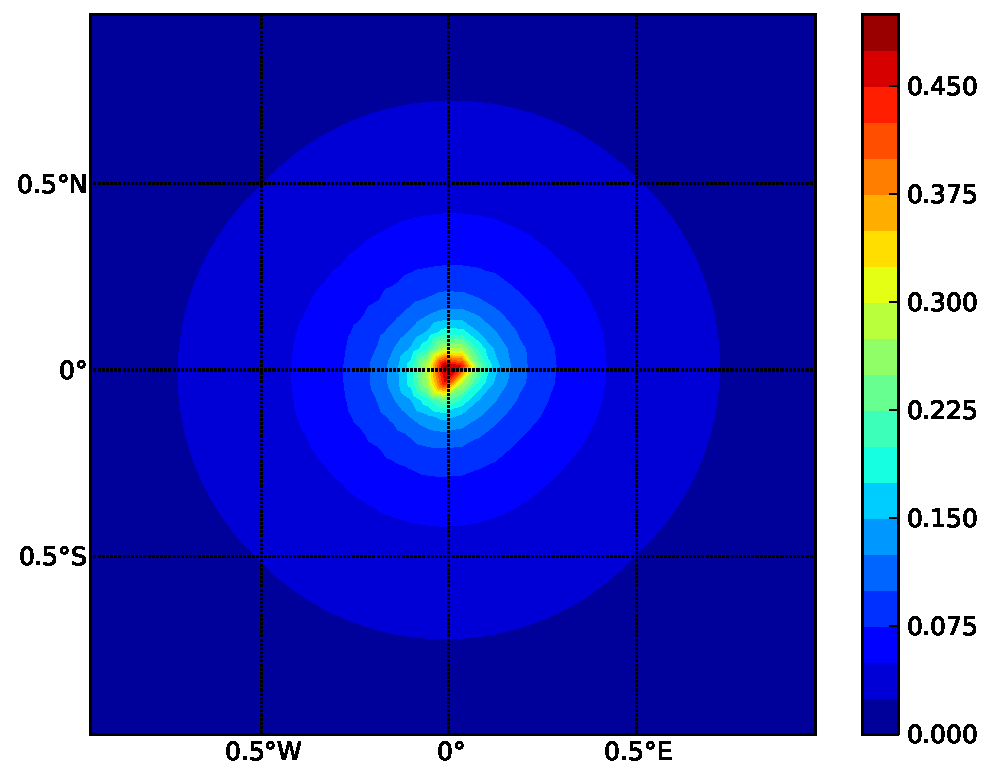
\includegraphics[width=7cm]{figures/hazard/point.pdf}}
\subcaptionbox{}
{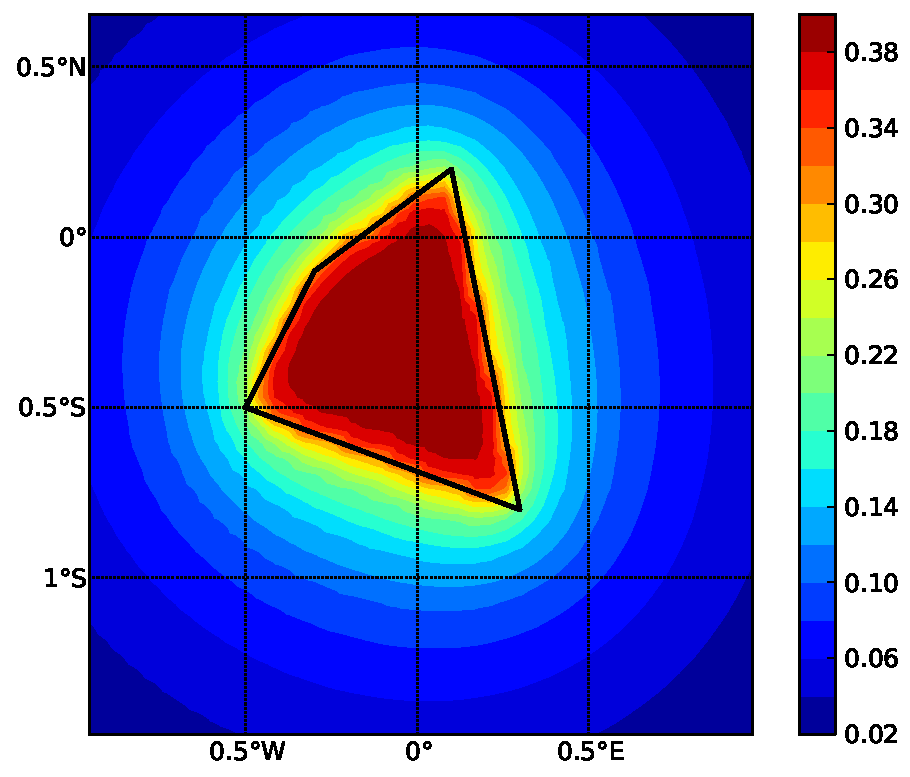
\includegraphics[width=7cm]{figures/hazard/area.pdf}} 
\subcaptionbox{}
{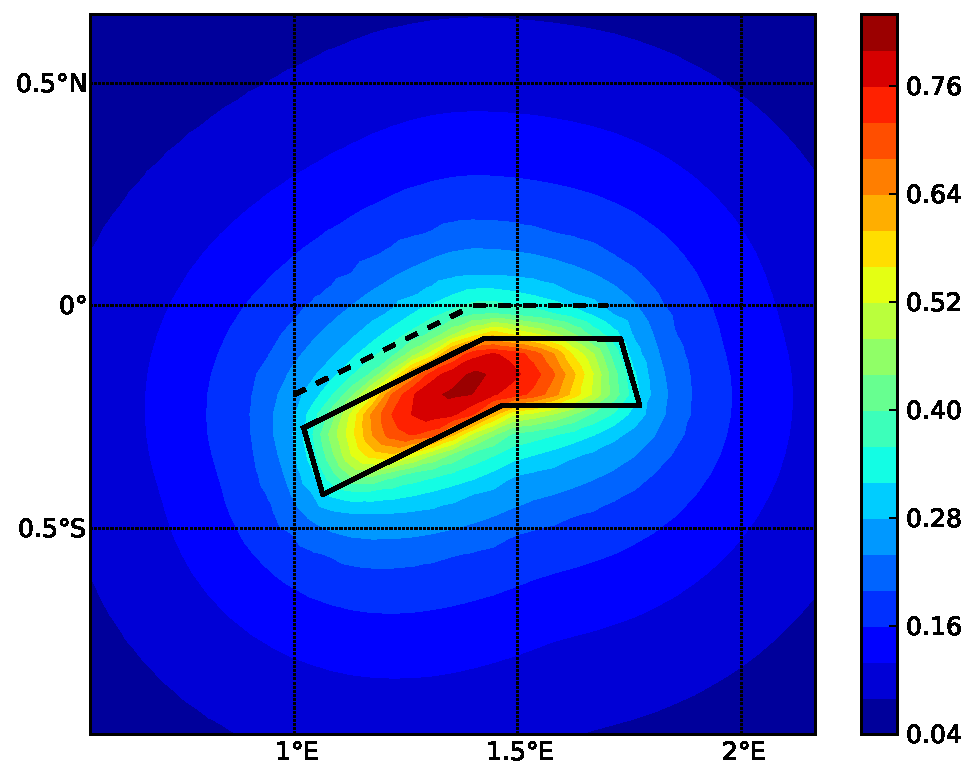
\includegraphics[width=7cm]{figures/hazard/simple_fault.pdf}} 
\subcaptionbox{}
{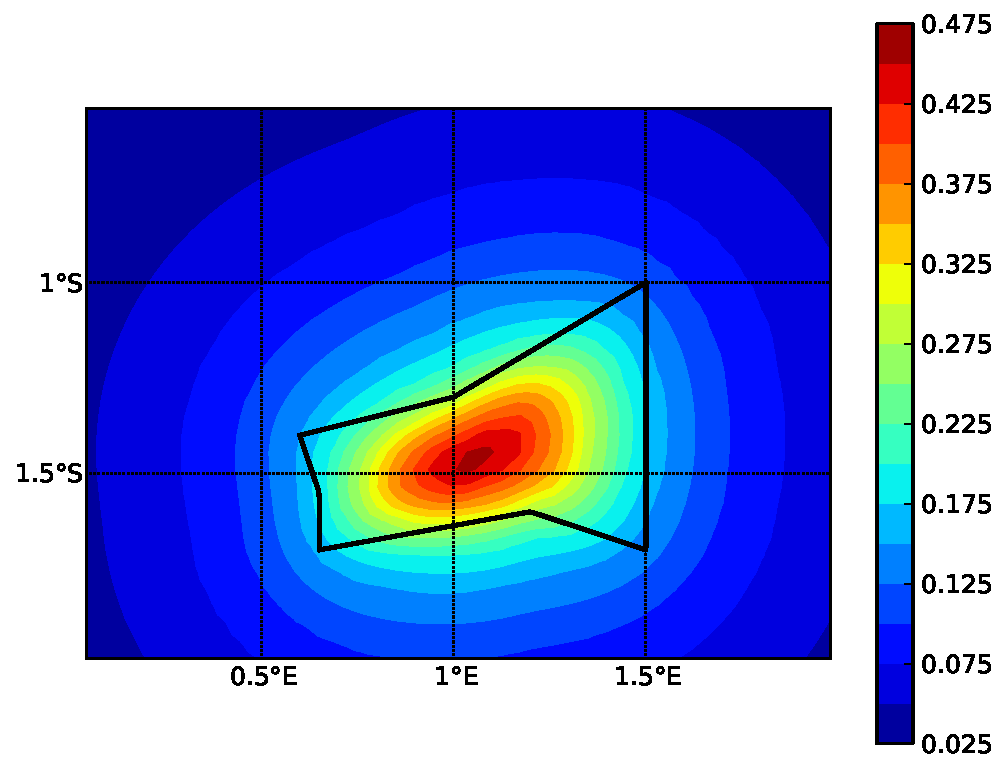
\includegraphics[width=7cm]{figures/hazard/complex_fault.pdf}} 
\caption{Hazard maps (for PGA, 10\% in 50 years) as obtained from the 
    different \gls{acr:oqe} source typologies. (a) Point Source. (b) Area 
    source.  The solid black line represents the area boundary. (c) Simple 
    Fault Source. 
    The dashed line represents the fault trace, while the solid line the fault
    surface projection. (d) Complex Fault Source. The solid line represent the 
    fault surface projection (d)}
\label{fig:hazard_maps1}
\end{figure}

\begin{figure} 
\centering 
\subcaptionbox{}
{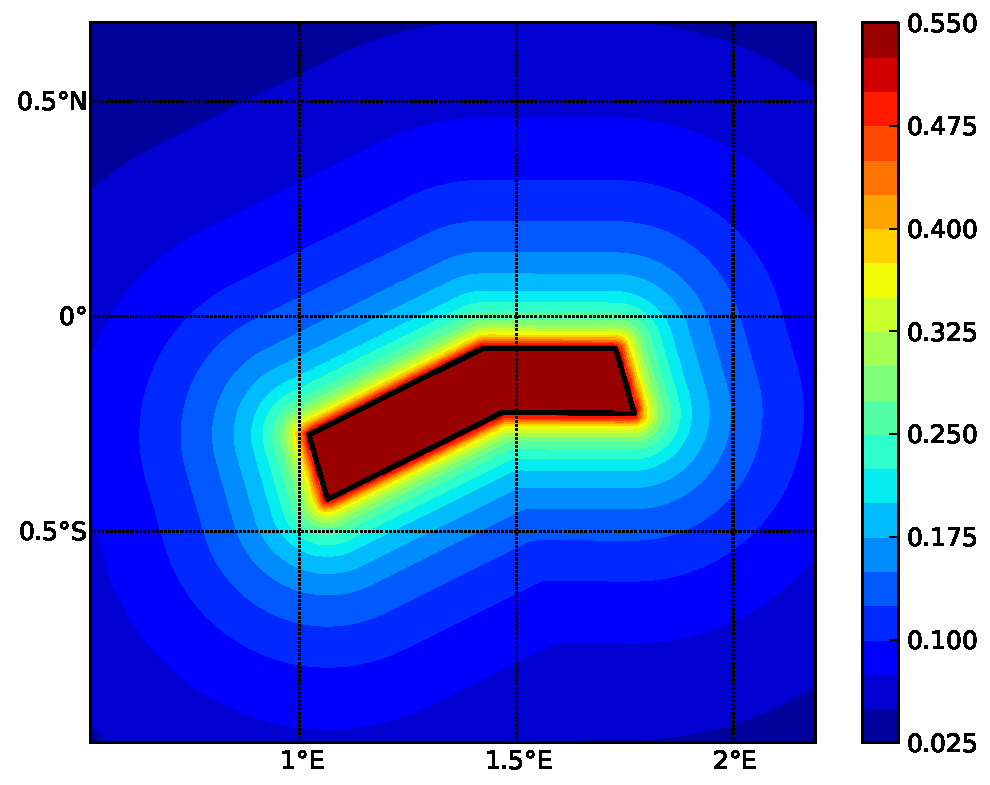
\includegraphics[width=7cm]{figures/hazard/char_fault2.pdf}} 
\subcaptionbox{}
{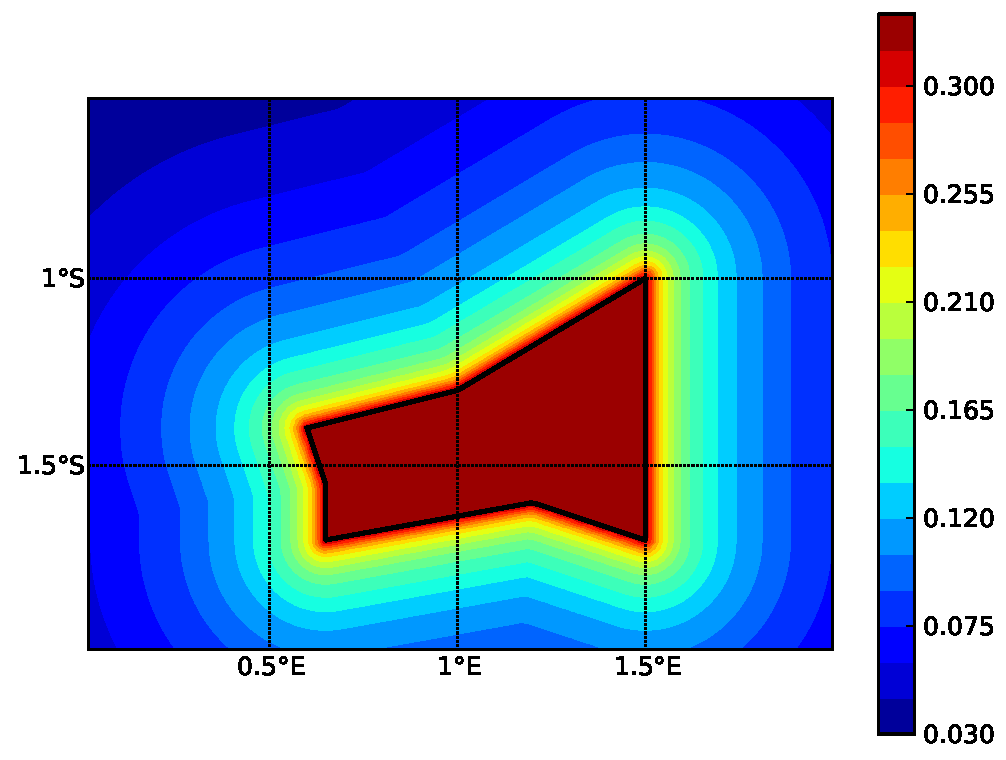
\includegraphics[width=7cm]{figures/hazard/char_fault3.pdf}} 
\subcaptionbox{}
{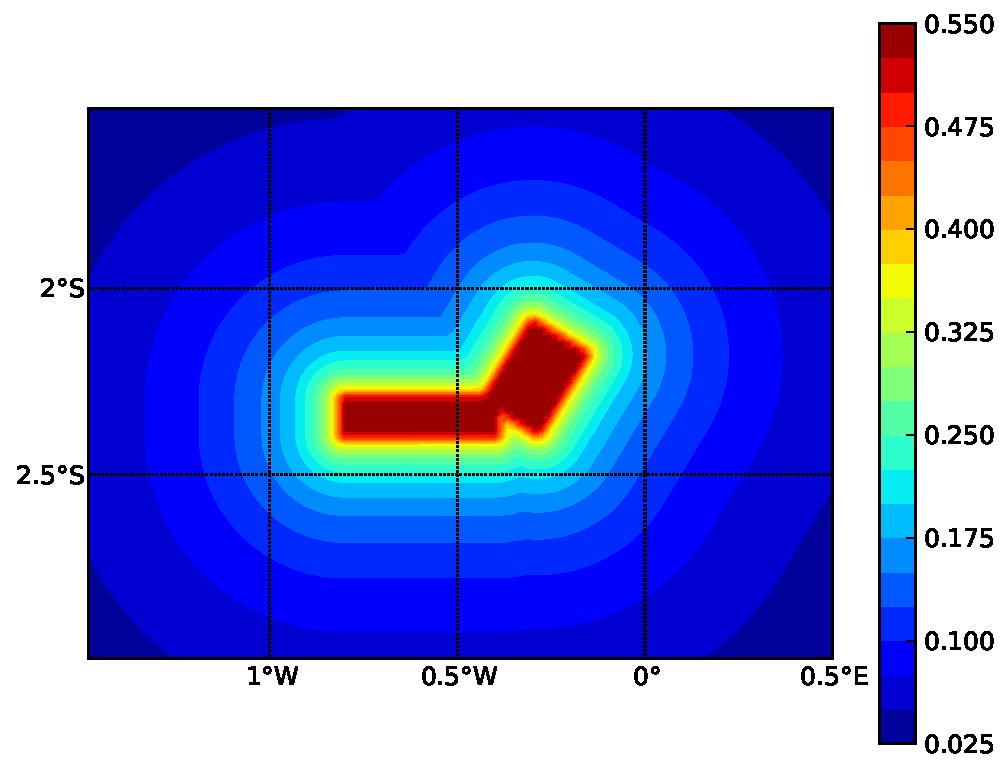
\includegraphics[width=7cm]{figures/hazard/char_fault1.pdf}} 
\caption{Hazard maps (for PGA, 10\% in 50 years) as obtained from 
    characteristic fault sources with simple fault
    geometry (a), complex fault geometry (b), and collection of
    planar surfaces (c)}
\label{fig:hazard_maps2}
\end{figure}

\clearpage
\subsection{Classical PSHA with non trivial logic trees}

Three demos are provided to illustrate how the logic tree formalism can be
used to express epistemic uncertainties in seismic hazard analysis.

LogicTreeCase1ClassicalPSHA shows an example of logic tree defining two
alternative source models, with sources belonging to two different tectonic
region types, and with two alternative GMPEs for each tectonic  region type.
The source model logic tree is therefore defined as shown in
Listing~\ref{lst:input_sslt_demo_LogicTreeCase1ClassicalPSHA}.

\begin{listing}[htbp]
  \inputminted[firstline=1,firstnumber=1,fontsize=\footnotesize,frame=single,linenos,bgcolor=lightgray]{xml}{oqum/hazard/verbatim/input_sslt_demo_LogicTreeCase1ClassicalPSHA.xml}
  \caption{Source model logic tree input file used in the LogicTreeCase1ClassicalPSHA demo}
  \label{lst:input_sslt_demo_LogicTreeCase1ClassicalPSHA}
\end{listing}

The two source models are defined in two separate files:
\texttt{source\_\-model\_\-1.xml} and \texttt{source\_\-model\_\-2.xml} each
one associated to a corresponding weight (0.5 for both).

The GSIM logic tree file contains the structure as shown in
Listing~\ref{lst:input_gmlt_demo_LogicTreeCase1ClassicalPSHA}.

\begin{listing}[htbp]
  \inputminted[firstline=1,firstnumber=1,fontsize=\footnotesize,frame=single,linenos,bgcolor=lightgray]{xml}{oqum/hazard/verbatim/input_gmlt_demo_LogicTreeCase1ClassicalPSHA.xml}
  \caption{GSIM logic tree input file used in the LogicTreeCase1ClassicalPSHA demo}
  \label{lst:input_gmlt_demo_LogicTreeCase1ClassicalPSHA}
\end{listing}

The source model contains sources belonging to Active Shallow Crust and
Stable Continental Crust, therefore the GSIM logic tree defines two branching
levels, one for each considered tectonic region type. Moreover for each
tectonic region a branch set with two GMPEs is defined: Boore and Atkinson
2008 and Chiou and Youngs 2008 for Active Shallow Crust and Toro et al. 2003
and Campbell 2003 for Stable Continental Crust. By processing the above logic
tree files using the logic tree path enumeration mode (enabled by setting in
the configuration file \texttt{number\_\-of\_\-logic\_\-tree\_\-samples = 0})
hazard results are computed for 8 logic tree paths (2 source models x 2 GMPEs
for Active x 2 GMPEs for Stable).

LogicTreeCase2ClassicalPSHA defines a single source model consisting of only
two sources (area and simple fault) belonging to different tectonic region
types (Active Shallow Crust and Stable Continental Region) and both
characterized by a truncated Gutenberg-Richter distribution. The logic tree
defines uncertainties for G-R a and b values (three possible pairs for each
source), maximum magnitude (three values for each source) and uncertainties
on the GMPEs for each tectonic region type (two GMPE per region type).

To accommodate such a structure the GSIM logic tree is defined as shown in
Listing~\ref{lst:input_gmlt_demo_LogicTreeCase2ClassicalPSHA}.

\begin{listing}[htbp]
  \inputminted[firstline=1,firstnumber=1,fontsize=\footnotesize,frame=single,linenos,bgcolor=lightgray]{xml}{oqum/hazard/verbatim/input_gmlt_demo_LogicTreeCase2ClassicalPSHA.xml}
  \caption{GSIM logic tree input file used in the LogicTreeCase2ClassicalPSHA demo}
  \label{lst:input_gmlt_demo_LogicTreeCase2ClassicalPSHA}
\end{listing}

The first branching level defines the source model. For each source, two
branching levels are created, one defining uncertainties on G-R a and b values
(defined by setting \texttt{uncertaintyType="abGRAbsolute"}) and G-R maximum
magnitude (\texttt{uncertaintyType="maxMagGRAbsolute"}).

It is important to notice that each branch set is applied to a specific source
by defining the attribute \texttt{apply\-To\-Sources}, followed by the source
ID. The GSIM logic tree file is the same as used for
LogicTreeCase1ClassicalPSHA. By setting in the configuration file
\texttt{number\_\-of\_\-logic\_\-tree\_\-samples = 0}, hazard results are
obtained for 324 paths (1 source model x 3 (a, b) pairs for source 1 x 3 (a,
b) pairs for source 2 x 3 max magnitude values for source 1 x 3 max magnitude
values for source 2 x 2 GMPEs for Active Shallow Crust X 2 GMPEs for Stable
Continental Crust), see Figure~\ref{fig:hazard_curves}.


\begin{figure}
\centering
\subcaptionbox{}
{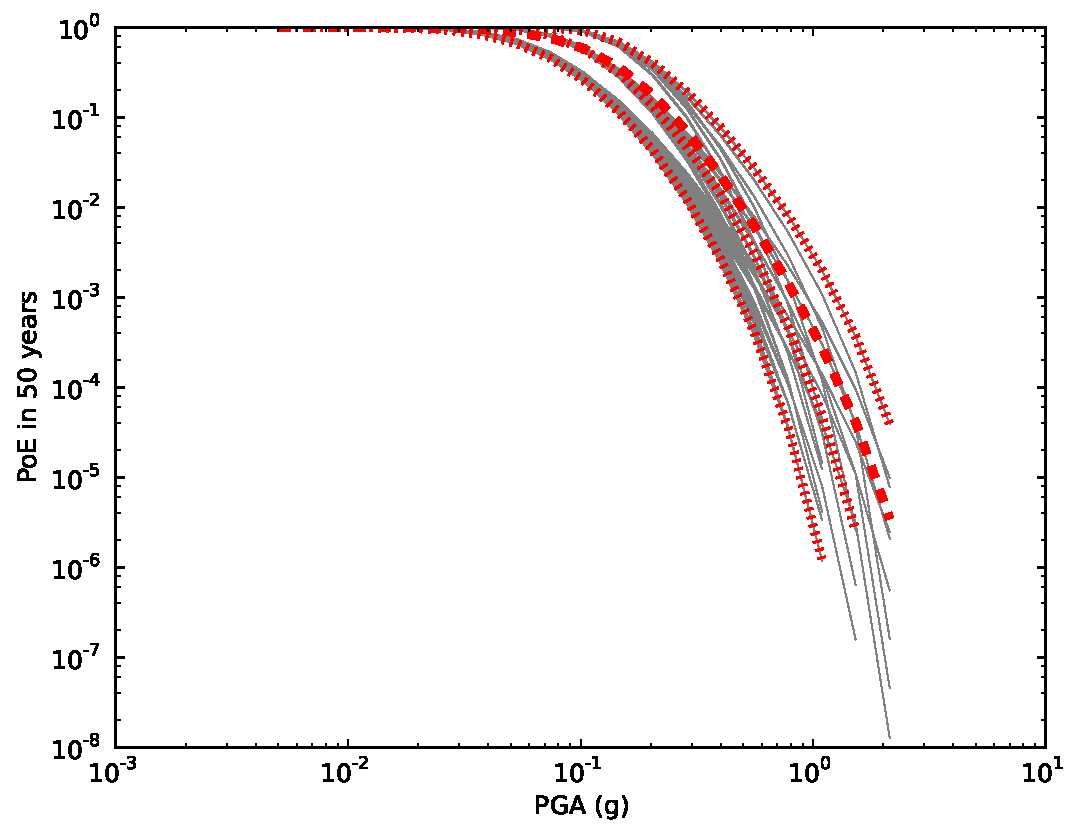
\includegraphics[width=9cm]{figures/hazard/hazard-curves-ltcase2.pdf}} 
\caption{Hazard curves as obtained from the LogicTreeCase2 demo. Solid gray 
    lines represent individual hazard curves from the different
    logic tree path (a total of 324 curves). The red dashed line represents the
    mean hazard curve, while the red dotted lines depict the quantile levels
    (0.15, 0.5, 0.95).}
\label{fig:hazard_curves}
\end{figure}

LogicTreeCase3ClassicalPSHA illustrates an example of logic tree defining
relative uncertainties on G-R maximum magnitude and b value. A single source
model is considered containing two sources belonging to different tectonic
region types and both characterized by a G-R magnitude frequency distribution.
The source model logic tree for this demo is as shown in
Listing~\ref{lst:input_sslt_demo_LogicTreeCase3ClassicalPSHA}.

\begin{listing}[htbp]
  \inputminted[firstline=1,firstnumber=1,fontsize=\footnotesize,frame=single,linenos,bgcolor=lightgray]{xml}{oqum/hazard/verbatim/input_sslt_demo_LogicTreeCase3ClassicalPSHA.xml}
  \caption{Source model logic tree input file used in the LogicTreeCase3ClassicalPSHA demos}
  \label{lst:input_sslt_demo_LogicTreeCase3ClassicalPSHA}
\end{listing}

After the first branching level defining the source model, two additional
branching levels are defined, one defining relative uncertainties on b value
(\texttt{bGRRelative} applied consistently to all sources in the source
model) and the second uncertainties on maximum magnitude
(\texttt{maxMagGRRelative}). Similar to the other cases, two GMPEs are
considered for each tectonic region type and therefore the total number of
logic tree path is 36 (1 source model x 3 b value increments x 3 maximum
magnitude increments x 2 GMPE for Active x 2 GMPEs for Stable).

\section{Hazard Disaggregation Demos}
\label{sec:demos_hazard_disaggregation}
An example of disaggregation calculation is given considering a source model
consisting of two sources (area and simple fault) belonging to two different
tectonic region types.

The calculation is defined with the following configuration file:

\begin{Verbatim}[frame=single, commandchars=\\\{\}, fontsize=\normalsize]
[general]
description = ...
calculation_mode = disaggregation
random_seed = 23

[geometry]
sites = 0.5 -0.5

[logic_tree]
number_of_logic_tree_samples = 0

[erf]
rupture_mesh_spacing = 2
width_of_mfd_bin = 0.1
area_source_discretization = 5.0

[site_params]
reference_vs30_type = measured
reference_vs30_value = 600.0
reference_depth_to_2pt5km_per_sec = 5.0
reference_depth_to_1pt0km_per_sec = 100.0

[calculation]
source_model_logic_tree_file = source_model_logic_tree.xml
gsim_logic_tree_file = gmpe_logic_tree.xml
investigation_time = 50.0
intensity_measure_types_and_levels = {"PGA": [...]}
truncation_level = 3
maximum_distance = 200.0

[disaggregation]
poes_disagg = 0.1
mag_bin_width = 1.0
distance_bin_width = 10.0
coordinate_bin_width = 0.2
num_epsilon_bins = 3

[output]
export_dir = ...
\end{Verbatim}

Disaggregation matrices are computed for a single site (located between the
two sources) for a ground motion value corresponding to a probability value
equal to 0.1 (\texttt{poes\_\-disagg = 0.1}). Magnitude values are classified
in one magnitude unit bins (\texttt{mag\_\-bin\_\-width = 1.0}), distances in
bins of 10 km (\texttt{distance\_\-bin\_\-width = 10.0}), coordinates in bins
of 0.2 degrees (\texttt{coordinate\_\-bin\_\-width = 0.2}). 3 epsilons bins
are considered (\texttt{num\_\-epsilon\_\-bins = 3}).


\section{Event Based PSHA Demos}
\label{sec:demos_event_based_psha}
A demo showing an example of Event Based PSHA calculation is provided with the
following configuration file:

\begin{Verbatim}[frame=single, commandchars=\\\{\}, fontsize=\normalsize]
[general]
description = Event Based PSHA using Area Source
calculation_mode = event_based
random_seed = 23

[geometry]
sites = 0.5 -0.5

[logic_tree]
number_of_logic_tree_samples = 0

[erf]
rupture_mesh_spacing = 2
width_of_mfd_bin = 0.1
area_source_discretization = 5.0

[site_params]
reference_vs30_type = measured
reference_vs30_value = 600.0
reference_depth_to_2pt5km_per_sec = 5.0
reference_depth_to_1pt0km_per_sec = 100.0

[calculation]
source_model_logic_tree_file = source_model_logic_tree.xml
gsim_logic_tree_file = gmpe_logic_tree.xml
investigation_time = 50.0
intensity_measure_types_and_levels = {"PGA": [...]}
truncation_level = 3
maximum_distance = 200.0

[event_based_params]
ses_per_logic_tree_path = 100
ground_motion_correlation_model =
ground_motion_correlation_params =

[output]
export_dir = ...
ground_motion_fields = true
hazard_curves_from_gmfs = true
mean_hazard_curves = false
quantile_hazard_curves =
hazard_maps = true
poes = 0.1
\end{Verbatim}

The source model consist of one source (area). 100 stochastic event sets  are
generated (\texttt{ses\_\-per\_\-logic\_\-tree\_\-path = 100}) (an example
can be seen in Figure~\ref{fig:ses}). Ground motion fields are computed
(\texttt{ground\_\-motion\_\-fields = true}, Figure~\ref{fig:gmfs}) and also
hazard curves from ground motion fields are extracted
(\texttt{hazard\_\-curves\_\-from\_\-gmfs = true}). The corresponding hazard
maps for 0.1 probability are also calculated (\texttt{hazard\_\-maps = true})

\begin{figure}
\centering
\subcaptionbox{}
{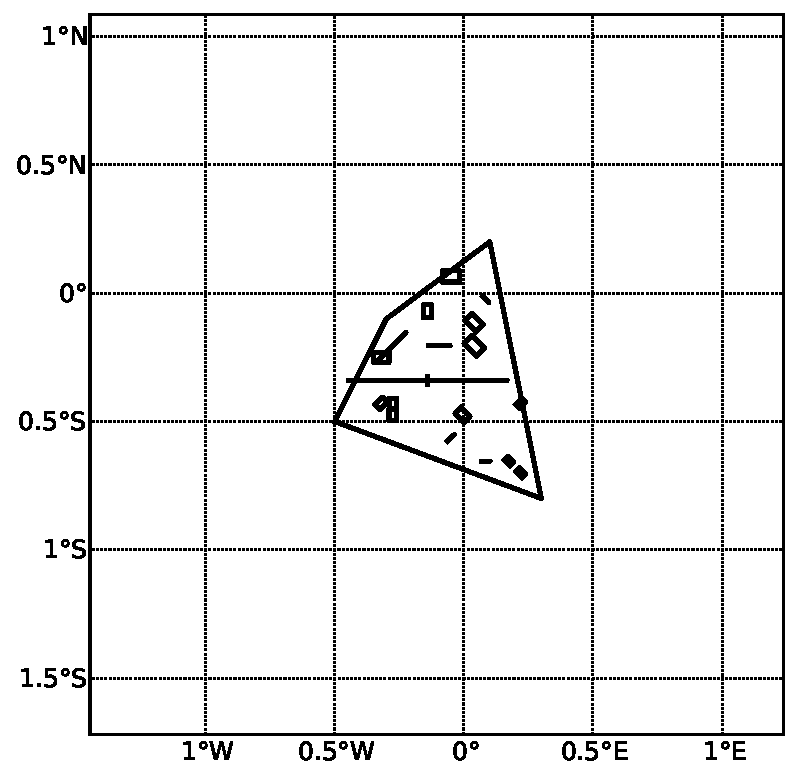
\includegraphics[width=9cm]{figures/hazard/ses.pdf}} 
\caption{A stochastic event set generated with the event based PSHA demo. 
    The area source defines a nodal plane distribution which distributes 
    events among vertical and dipping (50 degrees) faults with equal weights. 
    Vertical ruptures are then distributed equally in the range 0-180 degrees 
    while the dipping ones in the range 0-360, both with a step of 45 degrees.}
\label{fig:ses}
\end{figure}

\begin{figure}
\centering
\subcaptionbox{}
{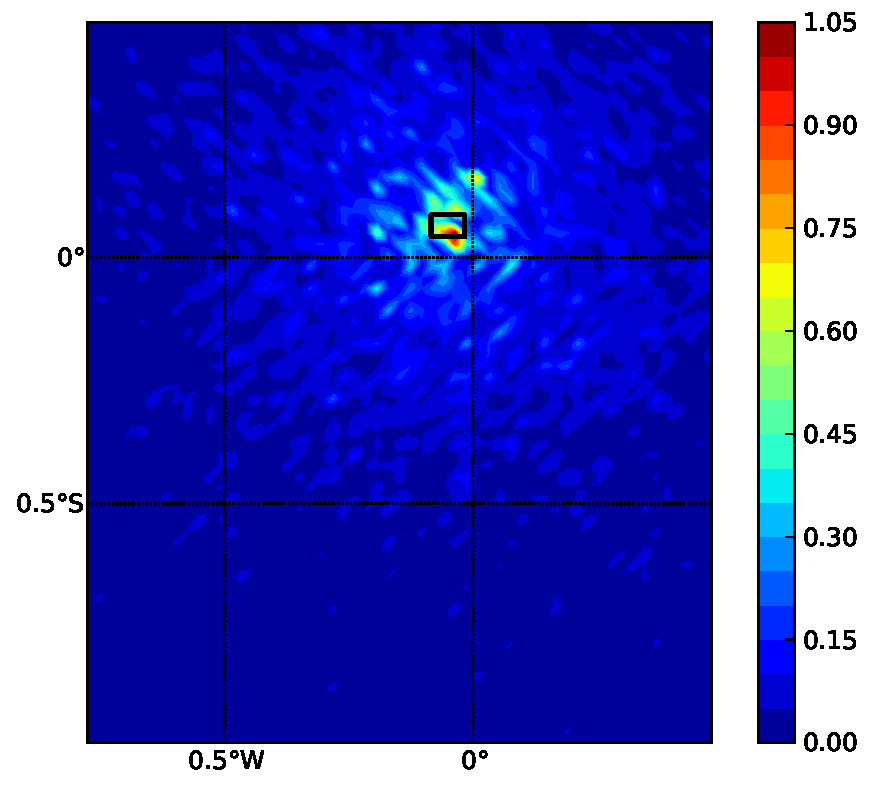
\includegraphics[width=6cm]{figures/hazard/gmf-no-corr.pdf}} 
\subcaptionbox{}
{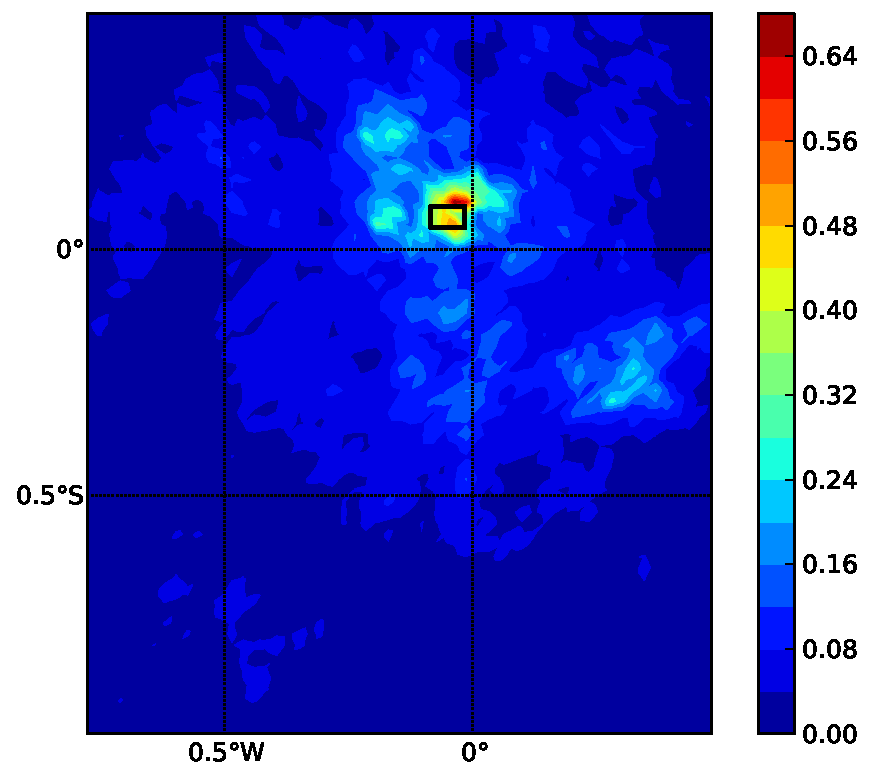
\includegraphics[width=6cm]{figures/hazard/gmf-corr.pdf}} 
\caption{Ground motion fields (PGA) with no spatial correlations (a) and with spatial correlation (b)}
\label{fig:gmfs}
\end{figure}

% \section{Scenario Hazard Demos}
% \label{sec:demos_scenario_hazard}
% \input{oqum/hazard/03d_scenario_demos}

   \cleardoublepage

% ------------------------------------------------------ Part III: Risk Module -
\thispagestyle{empty}
\part{Risk}

\chapterimage{figures/chapter_head.pdf} % Chapter heading image
\chapter{Introduction to the Risk Module}
   \label{chap:riskintro}
	\index{OpenQuake-engine!Hazard}

The hazard component of the \glsdesc{acr:oqe} builds on top of the
\gls{acr:hazlib}, a Python-based library containing tools for PSHA
calculations.

The web repository of this library is available at the following address:\\
\href{http://github.com/gem/oq-hazardlib}{http://github.com/gem/oq-hazardlib}.

In this section we briefly illustrate the main properties of the hazard
component of the \glsdesc{acr:oqe}. In particular, we will describe the main typologies of sources supported and the main calculation workflows available.


\section{Source typologies}
\index{Source type}
\label{sec:source_typologies}
An \glsdesc{acr:oqe} \gls{seismicsourceinputmodel} contains a list of sources
belonging to a finite set of possible typologies. Each source type is defined
by a set of parameters - called source data - which are used to specify the
source geometry and the properties of seismicity occurrence.

Currently the \glsdesc{acr:oqe} supports the following source types:

\begin{itemize}

    \item Sources for modelling distributed seismicity:

    \begin{itemize}

        \item \Gls{pointsource} - The elemental source type used to model
        distributed seismicity. Grid and area sources (described below) are
        different containers of point sources.

        \item \Gls{areasource} - So far, the most frequently adopted source
        type in national and regional PSHA models.

        \item \Gls{gridsource} - A replacement for area sources admitting
        spatially variable seismicity occurrence properties.

    \end{itemize}

    \item Fault sources with floating ruptures:

    \begin{itemize}

        \item \Gls{simplefaultsource} - The simplest fault model in the
        \glsdesc{acr:oqe}. This source is habitually used to describe shallow
        seismogenic faults.

        \item \Gls{complexfaultsource} - Often used to model subduction
        interface sources with a complex geometry.

    \end{itemize}

    \item Fault sources with ruptures always covering the entire fault surface:

    \begin{itemize}

        \item \Gls{charfaultsource} - A typology of source where ruptures
        always fill the entire fault surface.
        
        \item \Gls{nonparametricsource} - A typology of source representing
        a collection of ruptures, each with their associated probabilities
        of 0, 1, 2 ... occurrences in the investigation time

    \end{itemize}

    \item Sources for representing individual earthquake ruptures
    
    \begin{itemize}
        \item Planar fault rupture - an individual fault rupture represented as a single rectangular plane
        \item Multi-planar fault rupture - an individual rupture represented as a collection of rectangular planes
        \item Simple fault rupture - an individual fault rupture represented as a simple fault surface
        \item Complex fault rupture - an individual fault rupture represented as a complex fault surface
    \end{itemize}

\end{itemize}

The \glsdesc{acr:oqe} contains some basic assumptions for the definition of
these source typologies:

\begin{itemize}

    \item In the case of area and fault sources, the seismicity is
    homogeneously distributed over the source;

    \item Seismicity temporal occurrence follows a Poissonian model.

\end{itemize}

The above sets of sources may be referred to as ``parametric'' sources, that
is to say that the generation of the \Gls{earthquakeruptureforecast} is done
by the OpenQuake engine based on the parameters of the sources set by the
user. In some cases, particularly if the user wishes for the temporal
occurrence model to be non-Poissonian (such as the lognormal or Brownian
Passage Time models) a different type of behaviour is needed. For this
OpenQuake-engine supports a \Gls{nonparametricsource} in which the
\Gls{earthquakeruptureforecast} is provided explicitly by the user as a set of
ruptures and their corresponding probabilities of occurrence.

\subsection{Source typologies for modelling distributed seismicity}
\subsubsection{Point sources}
\label{subsubsec:point_sources}
\index{Source type!point}
\index{Point source|see{Source type}}

\begin{figure}[!ht]
\centering
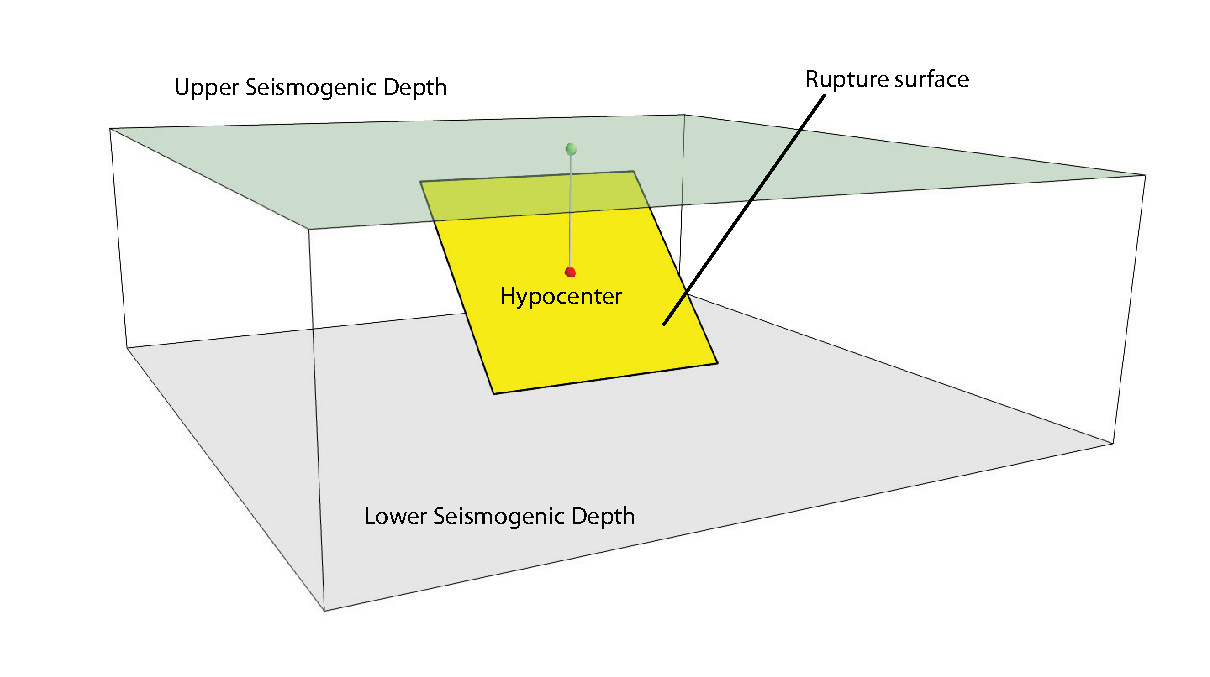
\includegraphics[width=10cm]{figures/hazard/single_rupture.pdf}
\caption{Single rupture}
\label{fig:single_rupture}
\end{figure}

The point source is the elemental source type adopted in the OpenQuake-engine
for modelling distributed seismicity. The \glsdesc{acr:oqe} always performs
calculations considering finite ruptures, even in the case of point sources.

These are the basic assumptions used to generate ruptures with point sources:

\begin{itemize}

    \item Ruptures have a rectangular shape

    \item Rupture hypocenter is located in the middle of the rupture

    \item Ruptures are limited at the top and at the bottom by two planes
    parallel to the sea level and placed at two characteristic
    depths named upper and lower seismogenic depths, respectively (see
    Figure~\ref{fig:single_rupture})

\end{itemize}

\paragraph{Source data}

For the definition of a point source the following parameters are required
(Figure~\ref{fig:single_rupture} shows some of the parameters described
below, together with an example of the surface of a generated rupture):

\begin{itemize}

    \item The coordinates of the point (i.e. longitude and latitude) [decimal
    degrees]

    \item The upper and lower seismogenic depths [km]

    \item One \gls{mfd}

    \item One magnitude-scaling relationship

    \item The rupture aspect ratio

    \item A distribution of nodal planes i.e. one (or several) instances
    of the following set of parameters:

    \begin{itemize}
        \item \gls{strike} [degrees]
        \item \gls{dip} [degrees]
        \item \gls{rake} [degrees]
    \end{itemize}

\item A magnitude independent depth distribution of hypocenters [km].

\end{itemize}

Figure~\ref{fig:point_source_multiple_ruptures} shows ruptures generated by a
point source for a range of magnitudes. Each rupture is centered on the
single hypocentral position admitted by this point source. Ruptures are
created by conserving the area computed using the specified magnitude-area
scaling relatioship and the corresponding value of magnitude.

\begin{figure}[ht!]
\centering
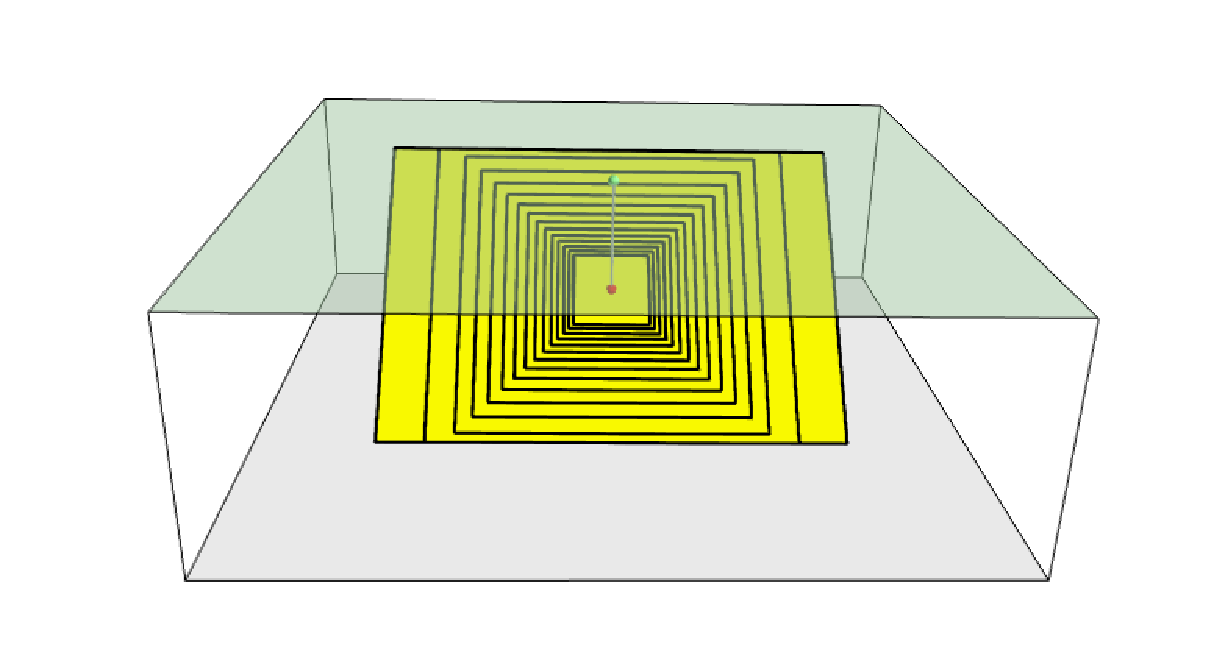
\includegraphics[width=10cm]{figures/hazard/point_source_multiple_ruptures.pdf}
\caption{Point source with multiple ruptures. Note the change in the aspect
ratio once the rupture width fills the entire seismogenic layer.}
\label{fig:point_source_multiple_ruptures}
\end{figure}

Below we provide the excerpt of an .xml file used to describe the properties of a point source. Note that in this example, ruptures occur on two possible nodal planes and two hypocentral depths. Figure~\ref{fig:point_source_ruptures} shows the ruptures generated by the point source.

\begin{listing}[htbp]
  \inputminted[firstline=1,firstnumber=1,fontsize=\footnotesize,frame=single,linenos,bgcolor=lightgray]{xml}{oqum/hazard/verbatim/input_point_source.xml}
  \caption{Example point source}
  \label{page:point_source_nrml}
\end{listing}

%The red part shows the the parameters used to describe the geometry of the point source, the blue part is the description of the magnitude-frequency distribution, the green text shows the nodal plane distribution and the text in magenta illustrates the hypocentral depth distribution.

%The text in black describes the parameters needed to generate the ruptures such as the \gls{msr} and the aspect ratio.



\begin{figure}[!ht]
\centering
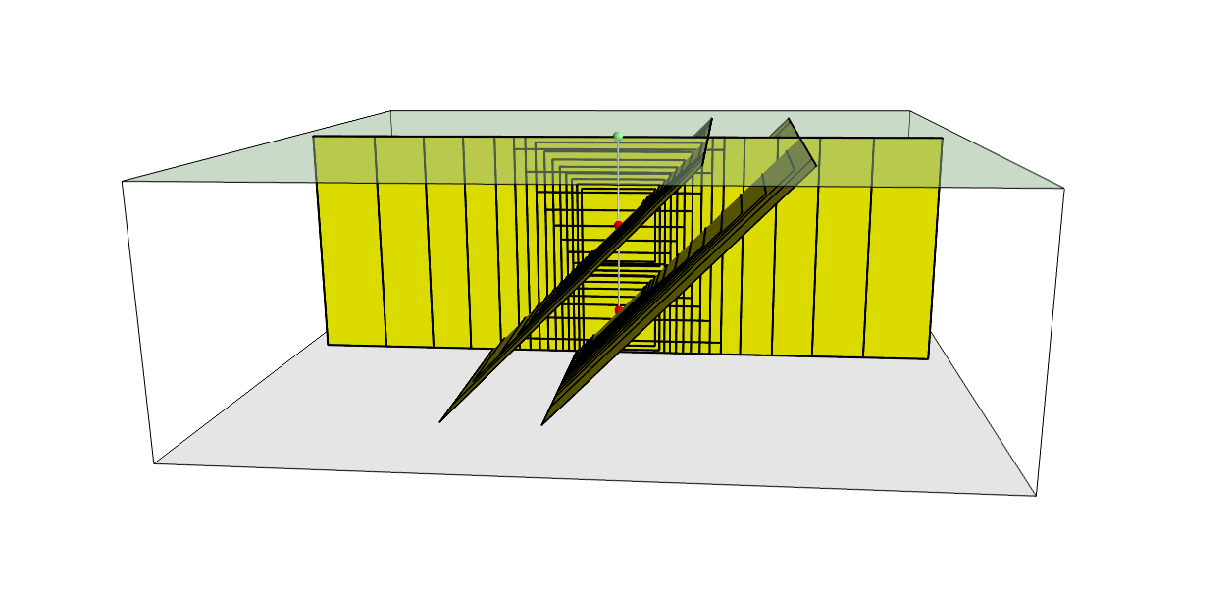
\includegraphics[width=10cm]{figures/hazard/pointsrc_2strike_2hypodep.pdf}
\caption{Ruptures produced by the source created using the information 
in the example .xml file described on page~\pageref{page:point_source_nrml}.}
\label{fig:point_source_ruptures}
\end{figure}

\subsubsection{Grid sources}
\label{subsubsec:grid_sources}
\index{Source type!grid}
\index{Grid source|see{Source type}}

A \gls{gridsource} is simply a collection of point sources distributed over a regular grid (usually equally spaced in longitude and latitude). In \gls{psha} a grid source can be considered a model alternative to area
sources, since they both model distributed seismicity. Grid sources are generally used to reproduce more faithfully the spatial pattern of seismicity depicted by the earthquakes occurred in the past; in
some models (e.g. \citet{petersen2008}) only events of low and intermediate magnitudes are considered. They are frequently, though not always, computed using seismicity smoothing algorithms \citep[][amongst many others]{frankel1995,woo1996}.

The use of smoothing algorithms to produce grid sources brings some
advantages compared to area sources, since (1) it removes most of the
unavoidable degree of subjectivity due to the definition of the geometries of the area sources and (2) it produces a spatial pattern of seismicity that is usually closer to what observed in the reality. Nevertheless, in many cases smoothing algorithms require an a-priori definition of some setup parameters that expose the calculation to a certain degree of partiality.

Grid sources are modeled in \gls{acr:oqe} simply as a set of point sources; in other words, a grid source is just a long list of point sources specified as described in the previous section (see page
\pageref{subsubsec:point_sources}).

\subsubsection{Area sources}
\label{subsubsec:area_sources}
\index{Source type!area}
\index{Area source|see{Source type}}

Area sources are usually adopted to describe the seismicity occurring over wide areas where the identification and characterization - i.e. the
unambiguous definition of position, geometry and seismicity occurrence
parameters - of single fault structures is difficult.

From a computation standpoint, area sources are comparable to grid sources since they are both represented in the engine by a list of point sources.

The \gls{acr:oqe} using the source data parameters (see below) creates an
equally spaced in distance grid of point sources where each point has the same seismicity occurrence properties (i.e. rate of events generated).

Below we provide a brief description of the parameters necessary to completely describe an area source.

\paragraph{Source data}

\begin{itemize}

    \item A polygon defining the external border of the area (i.e. a list of
    Longitude-Latitude [degrees] tuples) The current version of the OQ-engine doesn't
    support the definition of internal borders.

    \item The upper and lower seismogenic depths [km]

    \item One \gls{mfd}

    \item One \gls{msr}

    \item The rupture aspect ratio

    \item A distribution of nodal planes i.e. one (or several) instances of
    the following set of parameters

    \begin{itemize}
        \item \gls{strike} [degrees]
        \item \gls{dip} [degrees]
        \item \gls{rake} [degrees]
    \end{itemize}

    \item A magnitude independent depth distribution of hypocenters [km].

\end{itemize}

Below we provide the excerpt of an .xml file used to describe the properties of an area source. The ruptures generated by the area source described in the example are controlled by two nodal planes and have hypocenters at localized at two distinct depths.

\begin{listing}[htbp]
  \inputminted[firstline=1,firstnumber=1,fontsize=\footnotesize,frame=single,linenos,bgcolor=lightgray]{xml}{oqum/hazard/verbatim/input_area_source.xml}
  \caption{Example area source}
  \label{lst:area_source}
\end{listing}

%The red text describes the parameters used to describe the geometry of the area source; the blue part is the description of the magnitude-frequency distribution; the green text displays the nodal plane distribution; and the text in magenta illustrates the hypocentral depth distribution.

%The text in gray describes the parameters required to generate the ruptures such as the \gls{msr} and the aspect ratio.



\subsection{Fault sources with floating ruptures}
Fault sources in the \gls{acr:oqe} are classified according to the method
adopted to distribute ruptures over the fault surface. Two options are
currently supported:

\begin{itemize}

    \item With the first option, ruptures with a surface lower than the
    whole fault surface are floated so as to cover as much as possible
    homogeneously the fault surface. This model is compatible with all the
    supported magnitude-frequency distributions.

    \item With the second option, ruptures always fill the entire fault
    surface. This model is compatible with magnitude-frequency
    distributions similar to a characteristic model (\`{a} la
    \cite{schwartz1984}).

\end{itemize}

In this subsection we discuss the different fault source types that
support floating ruptures. In the next subsection we will illustrate the fault
typology available to model a characteristic rupturing behaviour.



\subsubsection{Simple faults}
\label{desc_simple_fault}
\index{Source type!fault!simple geometry}
\index{Simple fault|see{Source type}}

Simple Faults are the most common source type used to model shallow faults;
the ``simple'' adjective relates to the geometry description of the source
which is obtained by projecting the fault trace (i.e. a polyline) along a
characteristic dip direction.

The parameters used to create an instance of this source type are described
in the following paragraph.

\paragraph{Source data}

\begin{itemize}

    \item A horizontal \gls{faulttrace} (usually a polyline). It is a list of
    longitude-latitude tuples [degrees].

    \item A \gls{frequencymagnitudedistribution}

    \item A \gls{msr}

    \item A representative value of the dip angle (specified following
    the Aki-Richards convention; see \citet{aki2002}) [degrees]

    \item Rake angle (specified following the Aki-Richards convention;
    see \citet{aki2002}) [degrees]

    \item Upper and lower depth values limiting the seismogenic interval [km]

\end{itemize}

For near-fault probabilistic seismic hazard analysis, two additional
parameters are needed for characterising seismic sources:

\begin{itemize}

    \item A hypocentre list. It is a list of the possible hypocentral
    positions, and the corresponding weights, e.g., alongStrike="0.25"
    downDip="0.25" weight="0.25". Each hypocentral position is defined in
    relative terms using as a reference the upper left corner of the rupture
    and by specifying the fraction of rupture length and rupture width.

    \item A slip list. It is a list of the possible rupture slip directions
    [degrees], and their corresponding weights. The angle describing each slip
    direction is measured counterclockwise using the fault strike direction as
    reference.

\end{itemize}

In near-fault PSHA calculations, the hypocentre list and the slip list are
mandatory. The weights in each list must always sum to one. The available GMPE
which currently supports the near-fault directivity PSHA calculation in OQ-
engine is the ChiouYoungs2014NearFaultEffect GMPE developed  by
\citet{chiou2014update} (associated with an \texttt{Active Shallow Crust}
tectonic region type).

We provide two examples of simple fault source files. The first is an
excerpt of an xml file used to describe the properties of a simple fault
source and the second example shows the excerpt of an xml file used to
describe the properties of a simple fault source that can be used to perform a PSHA calculation taking into account directivity effects.

\begin{listing}[htbp]
  \inputminted[firstline=1,firstnumber=1,fontsize=\footnotesize,frame=single,linenos,bgcolor=lightgray]{xml}{oqum/hazard/verbatim/input_simple_fault.xml}
  \caption{Example simple fault}
  \label{lst:example_simple_fault}
\end{listing}
%\input{oqum/hazard/verbatim/input_simple_fault}
%\label{example_incremental_mfd}

%Below is an excerpt of a simple fault source xml file for near-fault directivity PSHA calculations:

%\begin{listing}[htbp]
\inputminted[firstline=1,firstnumber=1,fontsize=\footnotesize,frame=single,linenos,bgcolor=lightgray]{xml}{oqum/hazard/verbatim/input_simple_fault_directivity.xml}
\captionof{listing}{Example simple fault with added information to model directivity\label{lst:example_simple_fault_directivity}}

%\end{listing}

%\input{oqum/hazard/verbatim/input_simple_fault_directivity}

%As with the previous examples, the red text highlights the parameters used to specify the source geometry, the parameters in green describe the rupture mechanism, the text in blue describes the magnitude-frequency distribution and the gray text describes the rupture properties.



\subsubsection{Complex faults}
\label{desc_complex_fault}
\index{Source type!fault!complex geometry}
\index{Complex fault|see{Source type}}

A complex fault differs from simple fault just by the way the geometry of the
fault surface is defined and the fault surface is later created. The input
parameters used to describe complex faults are, for the most part, the same
used to describe the simple fault typology.

In the case of complex faults, the dip angle is not requested while the fault
trace is substituted by two fault edges limiting the top and bottom of the fault
surface. Additional curves lying over the fault surface can be specified to
complement and refine the description of the fault surface geometry.
Unlike the simple fault these edges are not required to be horizontal
and may vary in elevation, i.e. the upper edge may represent the intersection 
between the exposed fault trace and the topographic surface, where positive values
indicate below sea level, and negative values indicate above sea level.

Usually, we use complex faults to model intraplate megathrust faults such as
the big subduction structures active in the Pacific (Sumatra, South America,
Japan) but this source typology can be used also to create - for example -
listric fault sources with a realistic geometry.

\inputminted[firstline=1,firstnumber=1,fontsize=\footnotesize,frame=single,linenos,bgcolor=lightgray]{xml}{oqum/hazard/verbatim/input_complex_fault.xml}
\captionof{listing}{Example complex fault \label{lst:example_complex_fault}}

%\input{oqum/hazard/verbatim/input_complex_fault}

As with the previous examples, the red text highlights the parameters used to
specify the source geometry, the parameters in green describe the rupture
mechanism, the text in blue describes the magnitude-frequency distribution and
the gray text describes the rupture properties.


\subsection{Fault sources without floating ruptures}
\subsubsection{Characteristic faults}
\label{desc_characteristic_fault}
\index{Source type!fault!characteristic}
\index{Characteristic fault|see{Source type}}

The characteristic fault source is a particular typology of fault created
with the assumption that its ruptures will always cover the entire fault
surface. As such, no floating is necessary on the surface. The characteristic fault may still take as input a magnitude frequency distribution. In this case, the fault surface can be represented either as a \gls{simplefaultsource} surface or as a \gls{complexfaultsource} surface or as a combination of rectangular ruptures as represented in
Figure~\ref{fig:char_fault_source}. Mutiple surfaces containing mixed geometry types are also supported. 

\begin{figure}[htb]
\centering
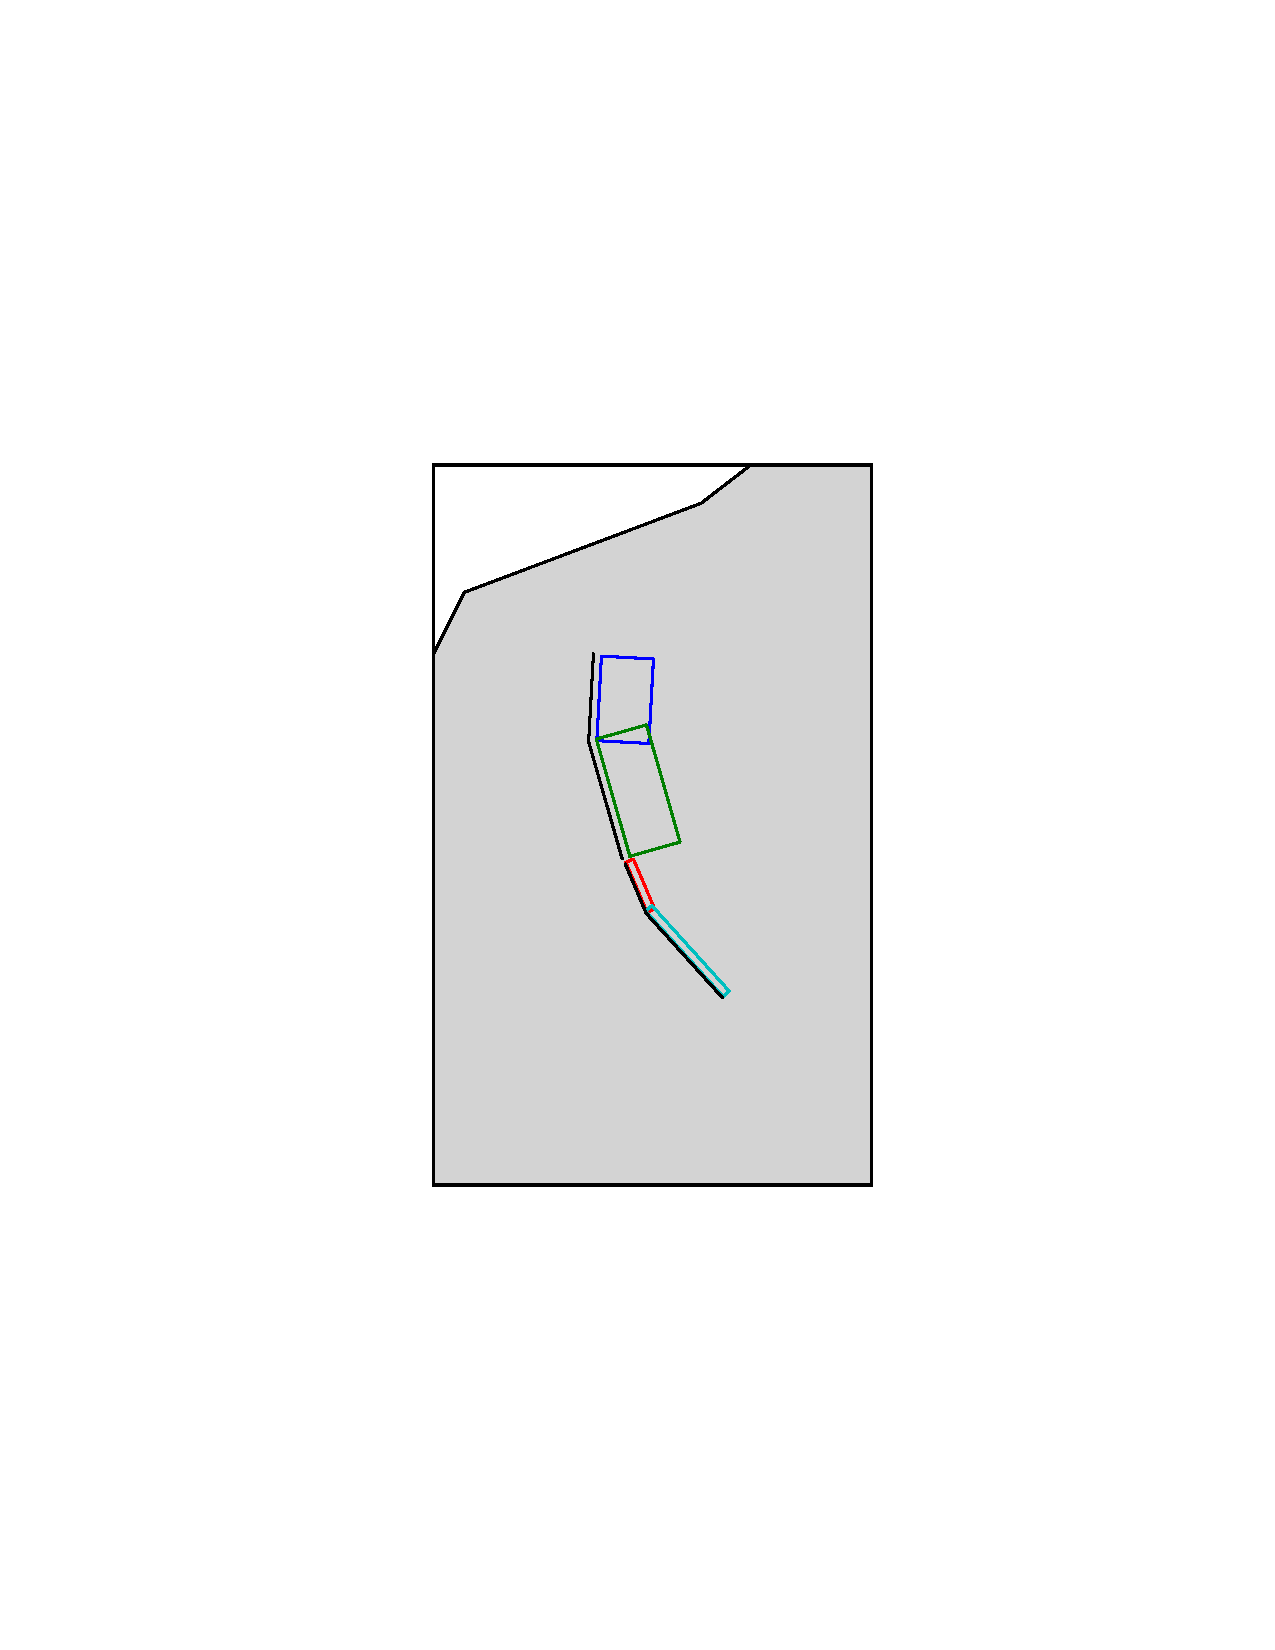
\includegraphics[trim=5cm 7cm 5cm 7cm, clip, width=10cm]{figures/hazard/multi_surface.pdf}
\caption{Geometry of a multi-segmented characteristic fault composed of four
         rectangular ruptures as modelled in OpenQuake.}
\label{fig:char_fault_source}
\end{figure}

\paragraph{Source data}
\begin{itemize}
    \item The characteristic rupture surface is defined through one of the
    following options:
        \begin{itemize}
            \item A list of rectangular ruptures (``planar surfaces'')
            \item A \gls{simplefaultsource} geometry
            \item A \gls{complexfaultsource} geometry
        \end{itemize}
    \item A \gls{frequencymagnitudedistribution}.
    \item Rake angle (specified following the Aki-Richards convention; see
          \citet{aki2002}).
    \item Upper and lower depth values limiting the seismogenic interval.
\end{itemize}

A comprehensive example enumerating the possible rupture surface configurations is shown below. 

\inputminted[firstline=1,firstnumber=1,fontsize=\footnotesize,frame=single,linenos,bgcolor=lightgray]{xml}{oqum/hazard/verbatim/input_characteristic_fault_simple.xml}
\captionof{listing}{Example characteristic fault with simple fault geometry\label{lst:example_characteristic_fault_simple}}

\inputminted[firstline=1,firstnumber=1,fontsize=\footnotesize,frame=single,linenos,bgcolor=lightgray]{xml}{oqum/hazard/verbatim/input_characteristic_fault_complex.xml}
\captionof{listing}{Example characteristic fault with complex fault geometry\label{lst:example_characteristic_fault_complex}}

\inputminted[firstline=1,firstnumber=1,fontsize=\footnotesize,frame=single,linenos,bgcolor=lightgray]{xml}{oqum/hazard/verbatim/input_characteristic_fault_planar.xml}
\captionof{listing}{Example characteristic fault with planar/multi-planar fault geometry\label{lst:example_characteristic_fault_planar}}



%\begin{mdframed}[]
%\inputminted[firstline=1,firstnumber=1,fontsize=%\footnotesize,frame=single,linenos,bgcolor=lightgray]{xml}{oqum/hazard/verbatim/input_nonparametric_source.xml}
%\caption{Example non-parametric source with planar, multi-planar, simple fault %and complex fault geometry}
%\label{lst:example_nonparametric_source}
%\end{mdframed}
%\input{oqum/hazard/verbatim/input_nonparametric_source}



\subsection{Non-Parametric Sources}
\subsubsection{Non-Parametric Fault}
\label{desc_nonparametric_fault}
\index{Source type!fault!nonparametric}
\index{Non-Parametric fault|see{Source type}}

The non-parametric fault typology requires that the user indicates the rupture properties (rupture surface, magnitude, rake and hypocentre) and the corresponding probabilities of the rupture. The probabilities are given as a list of floating point values that correspond to the probabilities of $0, 1, 2, \ldots ... N$ occurrences of the rupture within the specified investigation time. Note that there is not, at present, any internal check to ensure that the investigation time to which the probabilities refer corresponds to that specified in the configuration file. As the surface of the rupture is set explicitly, no rupture floating occurs, and, as in the case of the characteristic fault source, the rupture surface can be defined as either a single planar rupture, a list of planar ruptures, a \gls{simplefaultsource} geometry, a \gls{complexfaultsource} geometry, or a combination of different geometries.

Comprehensive examples enumerating the possible configurations are shown below:

\inputminted[firstline=1,firstnumber=1,fontsize=\footnotesize,frame=single,linenos,bgcolor=lightgray]{xml}{oqum/hazard/verbatim/input_nonparametric_planar.xml}
\captionof{listing}{Example non-parametric fault with planar and multi-planar fault geometry\label{lst:example_nonparametric_planar}}
\inputminted[firstline=1,firstnumber=1,fontsize=\footnotesize,frame=single,linenos,bgcolor=lightgray]{xml}{oqum/hazard/verbatim/input_nonparametric_simple.xml}
\captionof{listing}{Example characteristic fault with simple fault geometry\label{lst:example_nonparametric_simple}}
\inputminted[firstline=1,firstnumber=1,fontsize=\footnotesize,frame=single,linenos,bgcolor=lightgray]{xml}{oqum/hazard/verbatim/input_nonparametric_complex.xml}
\captionof{listing}{Example characteristic fault with complex fault geometry\label{lst:example_nonparametric_complex}}



\section{Magnitude-frequency distributions}
\label{sec:mfd_list}
The magnitude-frequency distributions currently supported by the
\gls{acr:oqe} are the following:

\begin{description}

\item[A discrete incremental magnitude-frequency distribution]
It is the simplest distribution supported. It is defined by the minimum value
of magnitude (representing the mid point of the first bin) and the bin width.
The distribution itself is simply a sequence of floats describing the annual
number of events for different bins. The maximum magnitude admitted by this
magnitude-frequency distribution is just the sum of the minimum magnitude and
the product of the bin width by the number annual rate values. Below we provide an example of the xml that should be incorporated in a
seismic source description in order to define this \gls{acr:mfd}.


\begin{minted}[firstline=1,firstnumber=1,fontsize=\footnotesize,frame=single,bgcolor=lightgray]{xml}
<incrementalMFD minMag="5.05" binWidth="0.1">
    <occurRates>0.15 0.08 0.05 0.03 0.015</occurRates>
</incrementalMFD>
\end{minted}

The magnitude-frequency distribution obtained with the above parameters is
represented in Figure~\ref{fig:evenly_discretized_mfd}.

\begin{figure}[!ht]
\centering
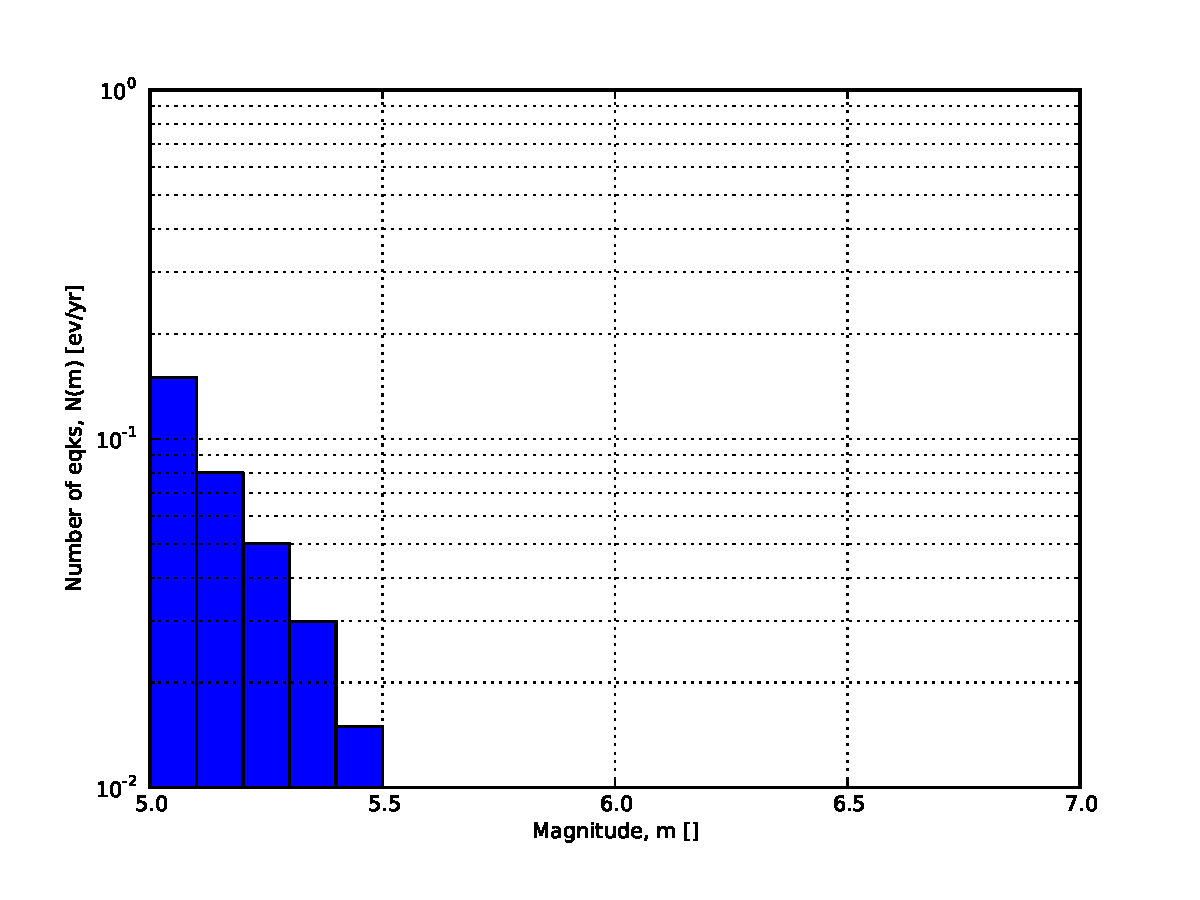
\includegraphics[width=12cm]{figures/hazard/ed_mfd.pdf}
\caption{Example of an incremental magnitude-frequency distribution.}
\label{fig:evenly_discretized_mfd}
\end{figure}

\item[A double truncated Gutenberg-Richter distribution]
This distribution is described by means of a minimum \texttt{minMag} and
maximum magnitude \texttt{maxMag} and by the $a$ and $b$ values of the
Gutenberg-Richter relationship.

The syntax of the xml used to describe this magnitude-frequency distribution
is rather compact as demonstrated in the following example:

\begin{minted}[firstline=1,firstnumber=1,fontsize=\footnotesize,frame=single,bgcolor=lightgray]{xml}
<truncGutenbergRichterMFD aValue="5.0" bValue="1.0" minMag="5.0"
                          maxMag="6.0"/>
\end{minted}

Figure~\ref{fig:dt_gr_mfd} shows the magnitude-frequency distribution
obtained using the parameters of the considered example.

\begin{figure}[!ht]
\centering
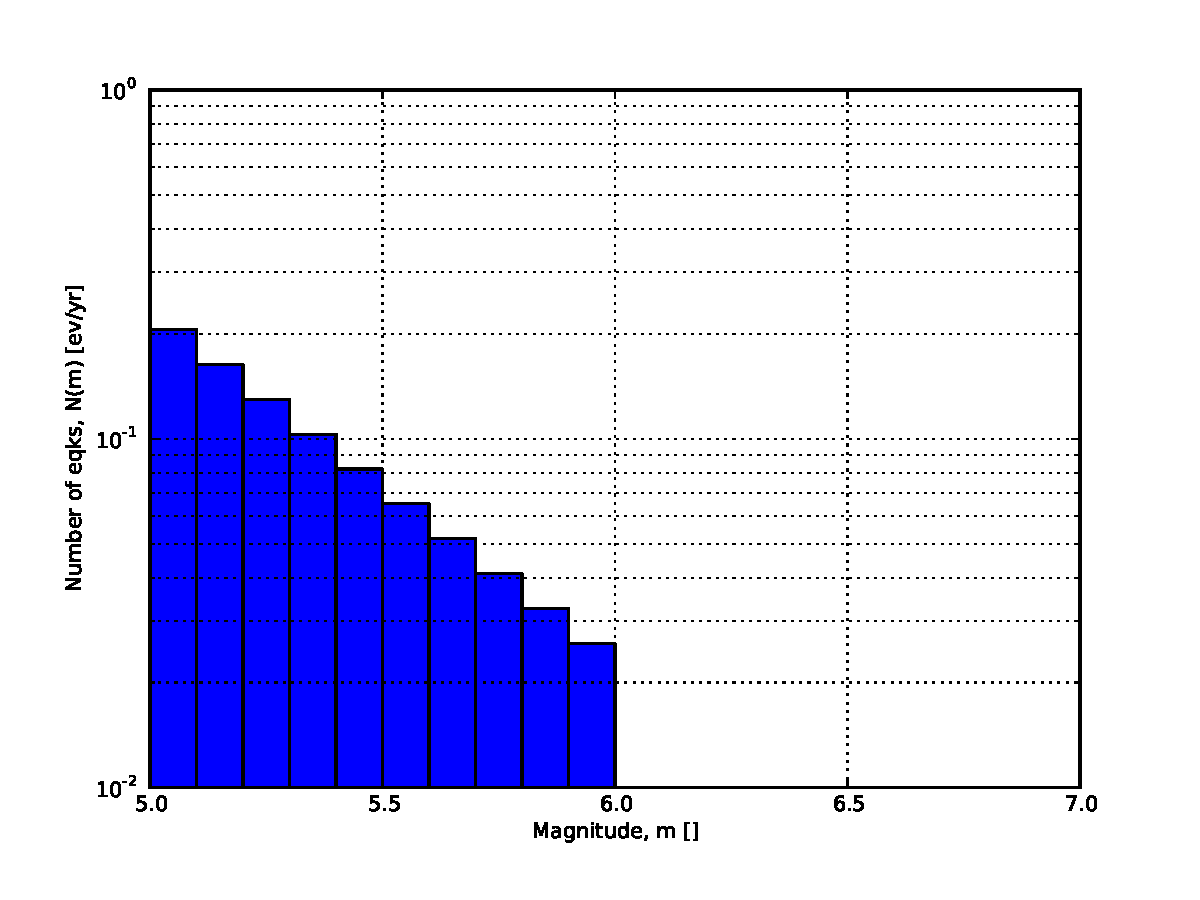
\includegraphics[width=12cm]{figures/hazard/dt_mfd.pdf}
\caption{Example of a double truncated Gutenberg-Richter magnitude-frequency
distribution.}
\label{fig:dt_gr_mfd}
\end{figure}

\item[Hybrid Characteristic earthquake model (\`{a} la \cite{youngs1985})]
The hybrid characteristic earthquake model, presented by \cite{youngs1985},
distributes seismic moment proportionally between a characteristic model (for
larger magnitudes) and an exponential model. The rate of events is dependent
on the magnitude of the characteristic earthquake, the b-value and the total
moment rate of the system (Figure \ref{fig:yc_gr_mfd}). However, the total
moment rate may be defined in one of two ways. If the total moment rate of the
source is known, as may be the case for a fault surface with known area and
slip rate, then the distribution can be defined from the total moment rate (in
N-m) of the source directly. Alternatively, the distribution can be defined
from the rate of earthquakes in the characteristic bin, which may be
preferable if the distribution is determined from observed seismicity
behaviour. The option to define the distribution according to the total moment
rate is input as:


\begin{minted}[firstline=1,firstnumber=1,fontsize=\footnotesize,frame=single,bgcolor=lightgray]{xml}
<YoungsCoppersmithMFD minmag="5.0" bValue="1.0" binWidth="0.1"
                      characteristicMag="7.0" totalMomentRate="1.05E19"/>
\end{minted}


\noindent whereas the option to define the distribution from the rate of
the characteristic events is given as:

\begin{minted}[firstline=1,firstnumber=1,fontsize=\footnotesize,frame=single,bgcolor=lightgray]{xml}
<YoungsCoppersmithMFD minmag="5.0" bValue="1.0" binWidth="0.1"
                      characteristicMag="7.0" characteristicRate="0.005"/>
\end{minted}

Note that in this distribution the width of the magnitude bin must be defined
explicitly in the model.

\begin{figure}[!ht]
\centering
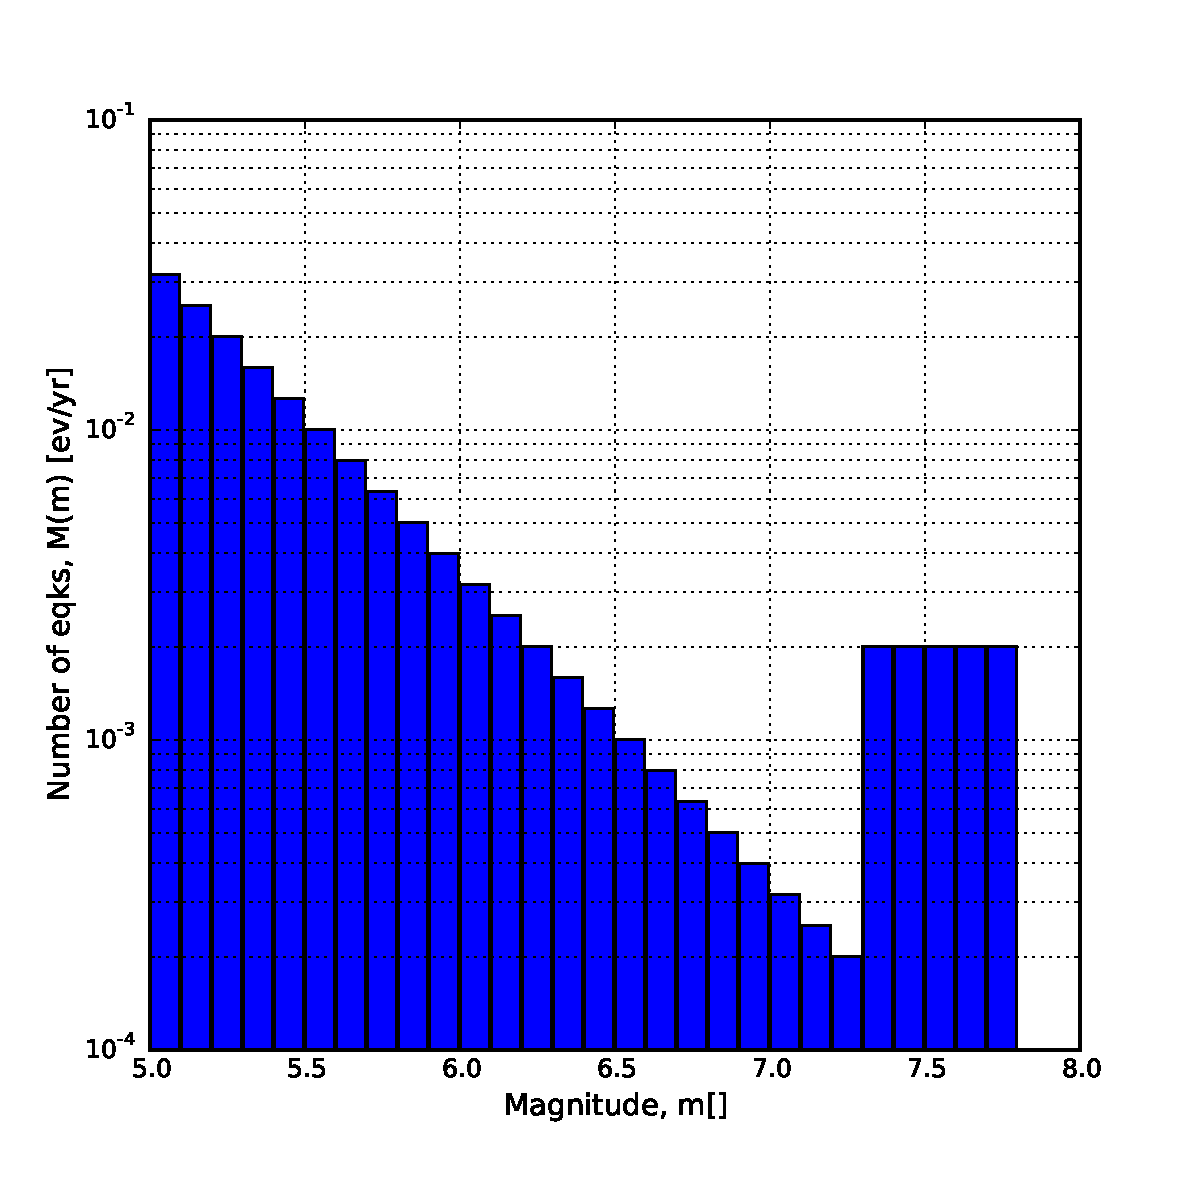
\includegraphics[width=10cm]{figures/hazard/yc_mfd_char_rate.pdf}
\caption{\cite{youngs1985} magnitude-frequency distribution.}
\label{fig:yc_gr_mfd}
\end{figure}

\item[``Arbitrary'' Magnitude Frequency Distribution]
The arbitrary magnitude frequency distribution is another non-parametric form
of MFD, in which the rates are defined explicitly. Here, the magnitude
frequency distribution is defined by a list of magnitudes and their
corresponding rates of occurrence. There is no bin-width as the rates
correspond exactly to the specific magnitude. Unlike the evenly discretised
MFD, there is no requirement that the magnitudes be equally spaced. This
distribution (illustrated in Figure \ref{fig:arb_mfd}) can be input as:

\begin{minted}[firstline=1,firstnumber=1,fontsize=\footnotesize,frame=single,bgcolor=lightgray]{xml}
<arbitraryMFD>
    <occurRates>0.12 0.036 0.067 0.2</occurRates>
    <magnitudes>8.1 8.47 8.68 9.02</magnitude>
</arbitraryMFD>
\end{minted}

\begin{figure}[!ht]
\centering
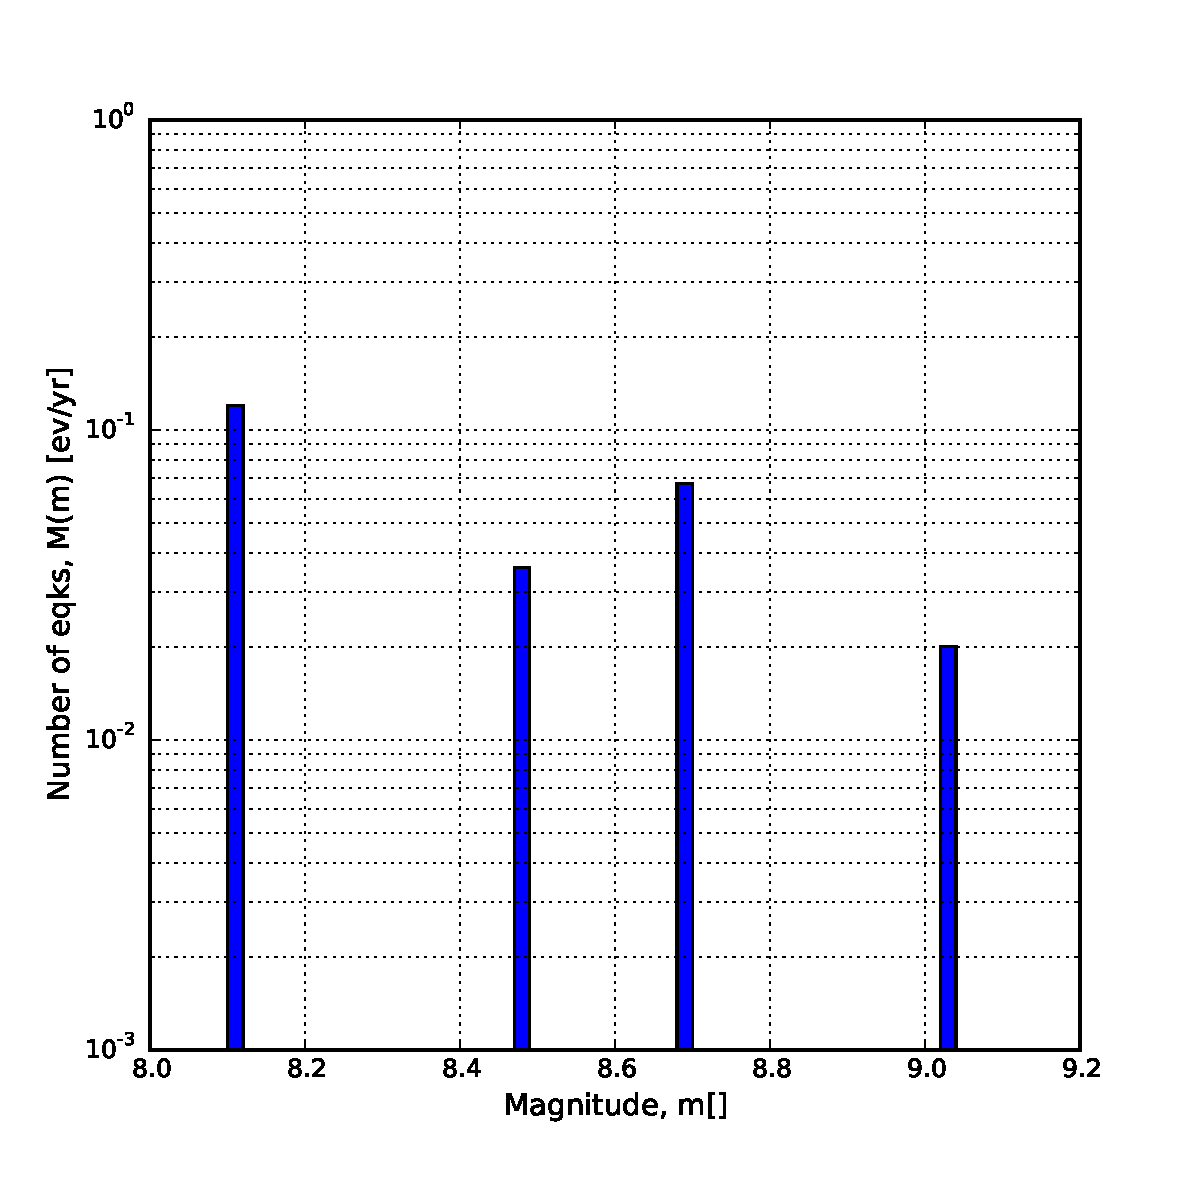
\includegraphics[width=10cm]{figures/hazard/arb_mfd.pdf}
\caption{``Arbitrary'' magnitude-frequency distribution.}
\label{fig:arb_mfd}
\end{figure}

\end{description}

\section{Magnitude-scaling relationships}
\label{sec:msr_list}
We provide below a list of the magnitude-area scaling relationships
implemented in the \gls{acr:hazlib}:

\subsection{Relationships for shallow earthquakes in active tectonic regions}

\begin{itemize}

    \item \cite{wells1994} - One of the most well known magnitude scaling
	relationships, based on a global database of historical earthquake
	ruptures. The implemented relationship is the one linking magnitude to
	rupture area, and is called with the keyword \verb=WC1994=

\end{itemize}


\subsection{Magnitude-scaling relationships for subduction earthquakes}
\begin{itemize}
    \item \cite{Strasser2010} - Defines several magnitude scaling relationships for interface and in-slab earthquakes. Only the magnitude to rupture-area scaling relationships are implemented here, and are called with the keywords \verb=StrasserInterface= and \verb=StrasserIntraslab= respectively.
    \item \cite{Thingbaijam2017} - Define  magnitude scaling relationships for interface. Only the magnitude to rupture-area scaling relationships are implemented here, and are called with the keywords \verb=ThingbaijamInterface=.
\end{itemize}

\subsection{Magnitude-scaling relationships stable continental regions}
\begin{itemize}
    \item \cite{ceus2011} - Defines a single magnitude to rupture-area scaling relationship for use in the central and eastern United States: $Area = 10.0^{M_W - 4.336}$. It is called with the keyword \verb=CEUS2011=
\end{itemize}

\subsection{Miscellaneous Magnitude-Scaling Relationships} 
\begin{itemize}
    \item \verb=PeerMSR= defines a simple magnitude scaling relation used as part of the Pacific Earthquake Engineering Research Center verification of probabilistic seismic hazard analysis programs: $Area = 10.0 ^{M_W - 4.0}$.
    \item \verb=PointMSR= approximates a `point' source by returning an infinitesimally small area for all magnitudes. Should only be used for distributed seismicity sources and not for fault sources. 
\end{itemize}

%
%\subsection{Ground motion prediction equations for volcanic areas}
%\begin{itemize}
%    \item
%\end{itemize}


\section{Calculation workflows}
\index{OpenQuake-engine!Hazard calculation workflows}
\label{sec:hazard_calculators}
The hazard component of the \glsdesc{acr:oqe} can compute seismic hazard using
various approaches. Three types of analysis are currently supported:

\begin{itemize}

	\item \textit{Classical Probabilistic Seismic Hazard Analysis (PSHA)},
	allowing calculation of hazard curves and hazard maps following the
	classical integration procedure (\cite{cornell1968}, \citet{mcguire1976})
	as formulated by \cite{field2003}.

	\item \textit{Event-Based Probabilistic Seismic Hazard Analysis},
	allowing calculation of ground-motion fields from stochastic event sets.
	Traditional results - such as hazard curves - can be obtained by post-
	processing the set of computed ground-motion fields.

	\item \textit{\gls{acr:ssha}}, allowing the calculation of ground
	motion fields from a single earthquake rupture scenario taking into
	account ground-motion aleatory variability.

\end{itemize}

Each workflow has a modular structure, so that intermediate results can be
exported and analyzed. Each calculator can be extended independently of the
others so that additional calculation options and methodologies can be easily
introduced, without affecting the overall calculation workflow.



\subsection{Classical Probabilistic Seismic Hazard Analysis}
\index{OpenQuake-engine!Hazard calculation workflows!Classical PSHA}
\label{subsec:classical_psha}
Input data for the classical \gls{acr:psha} consist of a PSHA input model
provided together with calculation settings.

The main calculators used to perform this analysis are the following:

\begin{enumerate}

	\item \emph{Logic Tree Processor}

	The Logic Tree Processor (LTP) takes as an input the \gls{acr:psha} Input
	Model and creates a Seismic Source Model. The LTP uses the information in
	the Initial Seismic Source Models and the Seismic Source Logic Tree to
	create a Seismic Source Input Model (i.e. a model describing geometry and
	activity rates of each source without any epistemic uncertainty).

	Following a procedure similar to the one just described the Logic Tree
	Processor creates a Ground Motion model (i.e. a data structure that
	associates to each tectonic region considered in the calculation a
	\gls{acr:gmpe}).

	\item \emph{Earthquake Rupture Forecast Calculator}

	The produced Seismic Source Input Model becomes an input information for
	the Earthquake Rupture Forecast (ERF) calculator which creates a list
	earthquake ruptures admitted by the source model, each one characterized
	by a probability of occurrence over a specified time span.

	\item \emph{Classical PSHA Calculator}

	The classical PSHA calculator uses the ERF and the Ground Motion model to
	compute hazard curves on each site specified in the calculation settings.

\end{enumerate}

\subsection{Event-Based Probabilistic Seismic Hazard Analysis}
\index{OpenQuake-engine!Hazard calculation workflows!Event-based PSHA}
\label{subsec:event_based_psha}
Input data for the Event-Based PSHA - as in the case of the Classical
\gls{acr:psha} calculator - consists of a PSHA Input Model and a set of
calculation settings.

The main calculators used to perform this analysis are:

\begin{enumerate}

	\item \emph{Logic Tree Processor}

	The Logic Tree Processor works in the same way described in  the
	description of the Classical \gls{acr:psha} workflow  (see
	Section~\ref{subsec:classical_psha} at
	page~\pageref{subsec:classical_psha}).

	\item \emph{Earthquake Rupture Forecast Calculator}

	The Earthquake Rupture Forecast Calculator was already  introduced in the
	description of the PSHA workflow (see Section~\ref{subsec:classical_psha}
	at page~\pageref{subsec:classical_psha}).

	\item \emph{Stochastic Event Set Calculator}

	The Stochastic Event Set Calculator generates a collection of stochastic
	event sets by sampling the ruptures contained in the ERF according to
	their probability of occurrence.

	A Stochastic Event Set (SES) thus represents a potential realisation of
	the seismicity (i.e. a list of ruptures) produced by the set of seismic
	sources considered in the analysis over the time span fixed for the
	calculation of hazard.

	\item \emph{Ground Motion Field Calculator}

	The Ground Motion Field Calculator computes for each event contained in a
	Stochastic Event Set a realization of the geographic distribution of the
	shaking by taking into account the aleatory uncertainties in the ground-
	motion model. Eventually, the Ground Motion Field calculator can consider
	the spatial correlation of the ground-motion during the generation of the
	\gls{acr:gmf}.

	\item \emph{Event-based PSHA Calculator}

	The event-based PSHA calculator takes a (large) set of ground-motion
	fields representative of the possible shaking scenarios that the
	investigated area can experience over a (long) time span and for each
	site computes the corresponding hazard curve.

	This procedure is computationally intensive and is not recommended for
	investigating the hazard over large areas.

\end{enumerate}

\subsection{Scenario based Seismic Hazard Analysis}
\index{OpenQuake-engine!Hazard calculation workflows!Scenario-based SHA}
\label{subsec:scenario_hazard}
In case of \gls{acr:ssha}, the input data consist of a single earthquake
rupture model and one or more ground-motion models. Using the Ground Motion
Field Calculator, multiple realizations of ground shaking can be computed,
each realization sampling the aleatory uncertainties in the ground-motion
model. The main calculator used to perform this analysis is the \emph{Ground
Motion Field Calculator}, which was already introduced during the description
of the event based PSHA workflow (see Section~\ref{subsec:event_based_psha} at
page~\pageref{subsec:event_based_psha}).

As the scenario calculator does not need to determine the probability of
occurrence of the specific rupture, but only sufficient information to
parameterise the location (as a three-dimensional surface), the magnitude and
the style-of-faulting of the rupture, a more simplified NRML structure is
sufficient compared to the source model structures described previously in
Section~\ref{sec:source_typologies}.
A \emph{rupture model} XML can be defined in the following formats:

\begin{enumerate}

    \item \emph{Simple Fault Rupture} - in which the geometry is defined by the
    trace of the fault rupture, the dip and the upper and lower seismogenic
    depths. An example is shown below in Listing~\ref{lst:input_rupture_simple}.

\begin{listing}[htbp]
  \inputminted[firstline=1,firstnumber=1,fontsize=\footnotesize,frame=single,linenos,bgcolor=lightgray]{xml}{oqum/hazard/verbatim/input_rupture_simple_fault.xml}
  \caption{An example simple fault rupture input file}
  \label{lst:input_rupture_simple}
\end{listing}

    \item \emph{Planar \& Multi-Planar Rupture} - in which the geometry is
    defined as a collection of one or more rectangular planes, each defined
    by four corners. An example of a multi-planar rupture is shown below
    in Listing~\ref{lst:input_rupture_multi_planes}.

\begin{listing}[htbp]
  \inputminted[firstline=1,firstnumber=1,fontsize=\footnotesize,frame=single,linenos,bgcolor=lightgray]{xml}{oqum/hazard/verbatim/input_rupture_multi_planes.xml}
  \caption{An example multi-planar rupture input file}
  \label{lst:input_rupture_multi_planes}
\end{listing}

    \item \emph{Complex Fault Rupture} - in which the geometry is defined by
    the upper, lower and (if applicable) intermediate edges of the fault
    rupture. An example of a complex fault rupture is shown below in
    Listing~\ref{lst:input_rupture_complex}.

\begin{listing}[htbp]
  \inputminted[firstline=1,firstnumber=1,fontsize=\footnotesize,frame=single,linenos,bgcolor=lightgray]{xml}{oqum/hazard/verbatim/input_rupture_complex.xml}
  \caption{An example complex fault rupture input file}
  \label{lst:input_rupture_complex}
\end{listing}

\end{enumerate}


\cleardoublepage
   \cleardoublepage

\chapterimage{figures/chapter_head.pdf} % Chapter heading image
\chapter{Risk Input Models}
   \label{chap:riskinputs}
   The following sections describe the basic inputs required for a risk
calculation, including \glspl{exposuremodel}, \glspl{fragilitymodel},
\glspl{consequencemodel}, and \glspl{vulnerabilitymodel}. In addition, each
risk calculator also requires the appropriate hazard inputs computed in the
region of interest. Hazard inputs include hazard curves for the classical
probabilistic damage and risk calculators, \gls{acr:gmf} for the scenario
damage and risk calculators, or \glspl{acr:ses} for the probabilistic event
based calculators.


\section{Exposure Models}
\label{sec:exposure}
\emph{All} risk calculators in the \glsdesc{acr:oqe} require an
\gls{exposuremodel} that needs to be provided in the \gls{acr:nrml} schema,
the use of which is illustrated through several examples in this section. The
information included in an \gls{exposuremodel} comprises a metadata section
listing general information about the exposure, followed by a cost conversions
section that describes how the different areas, costs, and occupancies for the
assets will be specified, followed by data regarding each individual
\gls{asset} in the portfolio.

A simple \gls{exposuremodel} comprising a single \gls{asset} is shown in
Listing~\ref{lst:input_exposure_minimal}.

\begin{listing}[htbp]
  \inputminted[firstline=1,firstnumber=1,fontsize=\footnotesize,frame=single,linenos,bgcolor=lightgray]{xml}{oqum/risk/verbatim/input_exposure_minimal.xml}
  \caption{Example exposure model comprising a single asset (\href{https://raw.githubusercontent.com/gem/oq-engine/master/doc/manual/oqum/risk/verbatim/input_exposure_minimal.xml}{Download example})}
  \label{lst:input_exposure_minimal}
\end{listing}

Let us take a look at each of the sections in the above example file in turn.
The first part of the file contains the metadata section:

\inputminted[firstline=5,firstnumber=5,lastline=8,fontsize=\footnotesize,frame=single,linenos,bgcolor=lightgray]{xml}{oqum/risk/verbatim/input_exposure_minimal.xml}

The information in the metadata section is common to all of the \glspl{asset}
in the portfolio and needs to be incorporated at the beginning of every
\gls{exposuremodel} file. There are a number of parameters that compose the
metadata section, which is intended to provide general information regarding
the \glspl{asset} within the \gls{exposuremodel}. These parameters are
described below:

\begin{itemize}

  \item \Verb+id+: mandatory; a unique string used to identify the
    \gls{exposuremodel}. This string can contain letters~(a--z; A--Z), 
    numbers~(0--9), dashes~(--), and underscores~(\_), with a maximum of 
    100~characters.

  \item \Verb+category+: an optional string used to define the type of
    \glspl{asset} being stored (e.g: buildings, lifelines).

  \item \Verb+taxonomySource+: an optional attribute used to define the
    \gls{taxonomy} being used to classify the \glspl{asset}.

  \item \Verb+description+: mandatory; a brief string (ASCII) with further
    information about the \gls{exposuremodel}.

\end{itemize}


Next, let us look at the part of the file describing the area and cost
conversions:

\inputminted[firstline=10,firstnumber=10,lastline=15,fontsize=\footnotesize,frame=single,linenos,bgcolor=lightgray]{xml}{oqum/risk/verbatim/input_exposure_minimal.xml}

Notice that the \Verb+costType+ element defines a \Verb+name+, a \Verb+type+, 
and a \Verb+unit+ attribute.

The \gls{acr:nrml} schema for the \gls{exposuremodel} allows the definition of
a structural cost, a nonstructural components cost, a contents cost, and a
business interruption or downtime cost for each \gls{asset} in the portfolio.
Thus, the valid values for the \Verb+name+ attribute of the \Verb+costType+
element are the following:

\begin{itemize}

  \item \Verb+structural+: used to specify the structural replacement cost
    of assets

  \item \Verb+nonstructural+: used to specify the replacement cost for the
    nonstructural components of assets

  \item \Verb+contents+: used to specify the contents replacement cost

  \item \Verb+business_interruption+: used to specify the cost that will be 
    incurred per unit time that a damaged asset remains closed following an 
    earthquake

\end{itemize}

The \gls{exposuremodel} shown in the example above defines only the structural
values for the \glspl{asset}. However, multiple cost types can be defined for
each \gls{asset} in the same \gls{exposuremodel}.

The \Verb+unit+ attribute of the \Verb+costType+ element is used for
specifying the currency unit for the corresponding cost type. Note that the
\glsdesc{acr:oqe} itself is agnostic to the currency units; the \Verb+unit+ is
thus a descriptive attribute which is used by the \glsdesc{acr:oqe} to annotate the
results of a risk assessment. This attribute can be set to any valid Unicode
string.

The \Verb+type+ attribute of the \Verb+costType+ element specifies whether the
costs will be provided as an aggregated value for an asset, or per building or
unit comprising an \gls{asset}, or per unit area of an \gls{asset}. The valid
values for the \Verb+type+ attribute of the \Verb+costType+ element are the
following:

\begin{itemize}

  \item \Verb+aggregated+: indicates that the replacement costs will be 
    provided as an aggregated value for each \gls{asset}

  \item \Verb+per_asset+: indicates that the replacement costs will be 
    provided per structural unit comprising each \gls{asset}

  \item \Verb+per_area+: indicates that the replacement costs will be 
    provided per unit area for each \gls{asset}

\end{itemize}

If the costs are to be specified \Verb+per_area+ for any of the
\Verb+costTypes+, the \Verb+area+ element will also need to be defined in the
conversions section. The \Verb+area+ element defines a \Verb+type+, and a
\Verb+unit+ attribute.

The \Verb+unit+ attribute of the \Verb+area+ element is used for specifying
the units for the area of an \gls{asset}. The \glsdesc{acr:oqe} itself is
agnostic to the area units; the \Verb+unit+ is thus a descriptive attribute
which is used by the \glsdesc{acr:oqe} to annotate the results of a risk
assessment. This attribute can be set to any valid ASCII string.

The \Verb+type+ attribute of the \Verb+area+ element specifies whether the
area will be provided as an aggregated value for an \gls{asset}, or per
building or unit comprising an \gls{asset}. The valid values for the
\Verb+type+ attribute of the \Verb+area+ element are the following:

\begin{itemize}

  \item \Verb+aggregated+: indicates that the area will be provided as an 
    aggregated value for each \gls{asset}

  \item \Verb+per_asset+: indicates that the area will be provided per 
    building or unit comprising each \gls{asset}

\end{itemize}


The way the information about the characteristics of the \glspl{asset} in an
\gls{exposuremodel} are stored can vary strongly depending on how and why the
data was compiled. As an example, if national census information is used to
estimated the distribution of \glspl{asset} in a given region, it is likely
that the number of buildings within a given geographical area will be used to
define the dataset, and will be used for estimating the number of collapsed
buildings for a scenario earthquake. On the other hand, if simplified
methodologies based on proxy data such as population distribution are used to
develop the \gls{exposuremodel}, then it is likely that the built up area or
economic cost of each building typology will be directly derived, and will be
used for the estimation of economic losses.


Finally, let us look at the part of the file describing the set of
\glspl{asset} in the portfolio to be used in seismic damage or risk
calculations:

\inputminted[firstline=17,firstnumber=17,lastline=27,fontsize=\footnotesize,frame=single,linenos,bgcolor=lightgray]{xml}{oqum/risk/verbatim/input_exposure_minimal.xml}

Each \gls{asset} definition involves specifiying a set of mandatory and
optional attributes concerning the \gls{asset}. The following set of
attributes can be assigned to each \gls{asset} based on the current schema for
the \gls{exposuremodel}:

\begin{itemize}

  \item \Verb+id+: mandatory; a unique string used to identify the 
    given \gls{asset}, which is used by the \glsdesc{acr:oqe} to relate each
    \gls{asset} with its associated results. This string can contain 
    letters~(a--z; A--Z), numbers~(0--9), dashes~(-), and underscores~(\_), 
    with a maximum of 100~characters.

  \item \Verb+taxonomy+: mandatory; this string specifies the building typology
    of the given \gls{asset}. The taxonomy strings can be user-defined, or
    based on an existing classification scheme such as the GEM Taxonomy, PAGER,
    or EMS-98.

  \item \Verb+number+: the number of individual structural units comprising a
    given \gls{asset}. This attribute is mandatory for damage calculations. For
    risk calculations, this attribute must be defined if either the area or any
    of the costs are provided per structural unit comprising each \gls{asset}.

  \item \Verb+area+: area of the \gls{asset}, at a given location. As 
    mentioned earlier, the area is a mandatory attribute only if any one of the 
    costs for the \gls{asset} is specified per unit area.

  \item \Verb+location+: mandatory; specifies the longitude 
    (between -180$^{\circ}$ to 180$^{\circ}$) and latitude 
    (between -90$^{\circ}$ to 90 $^{\circ}$) of the given \gls{asset}, both
    specified in decimal degrees\footnote{Within the \glsdesc{acr:oqe}, 
    longitude and latitude coordinates are internally rounded to a precision
    of 5 digits after the decimal point.}.

  \item \Verb+costs+: specifies a set of costs for the given \gls{asset}. 
    The replacement value for different cost types must be provided on 
    separate lines within the \Verb+costs+ element. As shown in the example 
    above, each cost entry must define the \Verb+type+ and the \Verb+value+. 
    Currently supported valid options for the cost \Verb+type+ are: 
    \Verb+structural+,  \Verb+nonstructural+, \Verb+contents+, and 
    \Verb+business_interruption+.

  \item \Verb+occupancies+: mandatory only for probabilistic or scenario 
    risk calculations that specify an \Verb+occupants_vulnerability_file+.
    Each entry within this element specifies the number of
    occupants for the asset for a particular period of the day. As shown in 
    the example above, each occupancy entry must define the \Verb+period+ and 
    the \Verb+occupants+. Currently supported valid options for the 
    \Verb+period+ are: \Verb+day+, \Verb+transit+, and \Verb+night+. Currently,
    the number of \Verb+occupants+ for an asset can only be provided as an 
    aggregated value for the asset.

\end{itemize}

For the purposes of performing a retrofitting benefit/cost analysis, it is
also necessary to define the retrofitting cost (\Verb+retrofitted+). The
combination between the possible options in which these three attributes can
be defined leads to four ways of storing the information about the
\glspl{asset}. For each of these cases a brief explanation and example is
provided in this section.


\paragraph{Example 1}

This example illustrates an \gls{exposuremodel} in which the aggregated cost
(structural, nonstructural, contents and business interruption) of the
\glspl{asset} of each taxonomy for a set of locations is directly provided.
Thus, in order to indicate how the various costs will be defined, the
following information needs to be stored in the \gls{exposuremodel} file, as
shown in Listing~\ref{lst:input_exposure_cagg_metadata}.

\begin{listing}[htbp]
  \inputminted[firstline=8,firstnumber=8,lastline=18,fontsize=\footnotesize,frame=single,linenos,bgcolor=lightgray]{xml}{oqum/risk/verbatim/input_exposure_cagg.xml}
  \caption{Example exposure model using aggregate costs: metadata definition (\href{https://raw.githubusercontent.com/gem/oq-engine/master/doc/manual/oqum/risk/verbatim/input_exposure_cagg.xml}{Download example})}
  \label{lst:input_exposure_cagg_metadata}
\end{listing}

In this case, the cost \Verb+type+ of each component as been defined as
\Verb+aggregated+. Once the way in which each cost is going to be defined has
been established, the values for each asset can be stored according to the
format shown in Listing~\ref{lst:input_exposure_cagg_assets}.

\begin{listing}[htbp]
  \inputminted[firstline=19,firstnumber=19,lastline=29,fontsize=\footnotesize,frame=single,linenos,bgcolor=lightgray]{xml}{oqum/risk/verbatim/input_exposure_cagg.xml}
  \caption{Example exposure model using aggregate costs: assets definition (\href{https://raw.githubusercontent.com/gem/oq-engine/master/doc/manual/oqum/risk/verbatim/input_exposure_cagg.xml}{Download example})}
  \label{lst:input_exposure_cagg_assets}
\end{listing}

Each \gls{asset} is uniquely identified by its \Verb+id+. Then, a pair of
coordinates (latitude and longitude) for a \Verb+location+ where the asset is
assumed to exist is defined. Each \gls{asset} must be classified according to
a \Verb+taxonomy+, so that the \glsdesc{acr:oqe} is capable of employing the
appropriate \gls{vulnerabilityfunction} or \gls{fragilityfunction} in the risk
calculations. Finally, the cost values of each \Verb+type+ are stored within
the \Verb+costs+ attribute. In this example, the aggregated value for all
structural units (within a given \gls{asset}) at each location is provided
directly, so there is no need to define other attributes such as \Verb+number+
or \Verb+area+. This mode of representing an \gls{exposuremodel} is probably
the simplest one.


\paragraph{Example 2}

In the snippet shown in Listing~\ref{lst:input_exposure_cunit_metadata}, an
\gls{exposuremodel} containing the number of structural units and the
associated costs per unit of each \gls{asset} is presented.

\begin{listing}[htbp]
  \inputminted[firstline=8,firstnumber=8,lastline=18,fontsize=\footnotesize,frame=single,linenos,bgcolor=lightgray]{xml}{oqum/risk/verbatim/input_exposure_cunit.xml}
  \caption{Example exposure model using costs per unit: metadata definition (\href{https://raw.githubusercontent.com/gem/oq-engine/master/doc/manual/oqum/risk/verbatim/input_exposure_cunit.xml}{Download example})}
  \label{lst:input_exposure_cunit_metadata}
\end{listing}

For this case, the cost \Verb+type+ has been set to \Verb+per_asset+. Then,
the information from each \gls{asset} can be stored following the format shown
in Listing~\ref{lst:input_exposure_cunit_assets}.

\begin{listing}[htbp]
  \inputminted[firstline=19,firstnumber=19,lastline=29,fontsize=\footnotesize,frame=single,linenos,bgcolor=lightgray]{xml}{oqum/risk/verbatim/input_exposure_cunit.xml}
  \caption{Example exposure model using costs per unit: assets definition (\href{https://raw.githubusercontent.com/gem/oq-engine/master/doc/manual/oqum/risk/verbatim/input_exposure_cunit.xml}{Download example})}
  \label{lst:input_exposure_cunit_assets}
\end{listing}

In this example, the various costs for each \gls{asset} is not provided
directly, as in the previous example. In order to carry out the risk
calculations in which the economic cost of each \gls{asset} is provided, the
\glsdesc{acr:oqe} multiplies, for each \gls{asset}, the number of units
(buildings) by the ``per asset'' replacement cost. Note that in this case,
there is no need to specify the attribute \Verb+area+.


\paragraph{Example 3}

The example shown in Listing~\ref{lst:input_exposure_carea_aagg_metadata}
comprises an \gls{exposuremodel} containing the built up area of each
\gls{asset}, and the associated costs are provided per unit area.

\begin{listing}[htbp]
  \inputminted[firstline=8,firstnumber=8,lastline=20,fontsize=\footnotesize,frame=single,linenos,bgcolor=lightgray]{xml}{oqum/risk/verbatim/input_exposure_carea_aagg.xml}
  \caption{Example exposure model using costs per unit area and aggregated areas: metadata definition (\href{https://raw.githubusercontent.com/gem/oq-engine/master/doc/manual/oqum/risk/verbatim/input_exposure_carea_aagg.xml}{Download example})}
  \label{lst:input_exposure_carea_aagg_metadata}
\end{listing}

In order to compile an \gls{exposuremodel} with this structure, the cost
\Verb+type+ should be set to \Verb+per_area+. In addition, it is also
necessary to specify if the \Verb+area+ that is being store represents the
aggregated area of number of units within an asset, or the average area of a
single unit. In this particular case, the \Verb+area+ that is being stored is
the aggregated built up area per asset, and thus this attribute was set to
\Verb+aggregated+. Listing~\ref{lst:input_exposure_carea_aagg_assets}
illustrates the definition of the \glspl{asset} for this example.

\begin{listing}[htbp]
  \inputminted[firstline=21,firstnumber=21,lastline=31,fontsize=\footnotesize,frame=single,linenos,bgcolor=lightgray]{xml}{oqum/risk/verbatim/input_exposure_carea_aagg.xml}
  \caption{Example exposure model using costs per unit area and aggregated areas: assets definition (\href{https://raw.githubusercontent.com/gem/oq-engine/master/doc/manual/oqum/risk/verbatim/input_exposure_carea_aagg.xml}{Download example})}
  \label{lst:input_exposure_carea_aagg_assets}
\end{listing}

Once again, the \glsdesc{acr:oqe} needs to carry out some calculations in
order to compute the different costs per \gls{asset}. In this case, this value
is computed by multiplying the aggregated built up \Verb+area+ of each
\gls{asset} by the associated cost per unit area. Notice that in this case,
there is no need to specify the attribute \Verb+number+.


\paragraph{Example 4}

This example demonstrates an \gls{exposuremodel} that defines the number of
structural units for each \gls{asset}, the average built up area per
structural unit and the associated costs per unit area.
Listing~\ref{lst:input_exposure_carea_aunit_metadata} shows the metadata
definition for an \gls{exposuremodel} built in this manner.

\begin{listing}[htbp]
  \inputminted[firstline=8,firstnumber=8,lastline=20,fontsize=\footnotesize,frame=single,linenos,bgcolor=lightgray]{xml}{oqum/risk/verbatim/input_exposure_carea_aunit.xml}
  \caption{Example exposure model using costs per unit area and areas per unit: metadata definition (\href{https://raw.githubusercontent.com/gem/oq-engine/master/doc/manual/oqum/risk/verbatim/input_exposure_carea_aunit.xml}{Download example})}
  \label{lst:input_exposure_carea_aunit_metadata}
\end{listing}

Similarly to what was described in the previous example, the various costs
\Verb+type+ also need to be established as \Verb+per_area+, but the
\Verb+type+ of area is now defined as \Verb+per_asset+.
Listing~\ref{lst:input_exposure_carea_aunit_assets} illustrates the definition
of the assets for this example.

\begin{listing}[htbp]
  \inputminted[firstline=21,firstnumber=21,lastline=31,fontsize=\footnotesize,frame=single,linenos,bgcolor=lightgray]{xml}{oqum/risk/verbatim/input_exposure_carea_aunit.xml}
  \caption{Example exposure model using costs per unit area and areas per unit: assets definition (\href{https://raw.githubusercontent.com/gem/oq-engine/master/doc/manual/oqum/risk/verbatim/input_exposure_carea_aunit.xml}{Download example})}
  \label{lst:input_exposure_carea_aunit_assets}
\end{listing}

In this example, the \glsdesc{acr:oqe} will make use of all the parameters to
estimate the various costs of each \gls{asset}, by multiplying the number of
structural units by its average built up area, and then by the respective cost
per unit area.


\paragraph{Example 5}

In this example, additional information will be included, which is required
for other risk analysis besides loss estimation, such as the calculation of
insured losses or benefit/cost analysis. For the calculation of insured
losses, it is necessary to establish how the insurance \glspl{limit} and
\glspl{deductible} are going to be defined.
Listing~\ref{lst:input_exposure_ins_rel_metadata} illustrates the metadata
section of an \gls{exposuremodel} where the insurance \glspl{limit} and
\glspl{deductible} for structural components will be defined relative to the
structural replacement cost.

\begin{listing}[htbp]
  \inputminted[firstline=8,firstnumber=8,lastline=21,fontsize=\footnotesize,frame=single,linenos,bgcolor=lightgray]{xml}{oqum/risk/verbatim/input_exposure_ins_rel.xml}
  \caption{Example exposure model using relative insurance limits and deductibles: metadata definition (\href{https://raw.githubusercontent.com/gem/oq-engine/master/doc/manual/oqum/risk/verbatim/input_exposure_ins_rel.xml}{Download example})}
  \label{lst:input_exposure_ins_rel_metadata}
\end{listing}

In this example, both the insurance \gls{limit} and the \gls{deductible} are
defined as a fraction of the replacement cost, by setting the attribute
\Verb+isAbsolute+ to \Verb+false+. Then, for each type of cost, the
\gls{limit} and \gls{deductible} value can be stored for each asset, as
illustrated in the snippet shown in
Listing~\ref{lst:input_exposure_ins_rel_assets}.

\begin{listing}[htbp]
  \inputminted[firstline=22,firstnumber=22,lastline=32,fontsize=\footnotesize,frame=single,linenos,bgcolor=lightgray]{xml}{oqum/risk/verbatim/input_exposure_ins_rel.xml}
  \caption{Example exposure model using relative insurance limits and deductibles: assets definition (\href{https://raw.githubusercontent.com/gem/oq-engine/master/doc/manual/oqum/risk/verbatim/input_exposure_ins_rel.xml}{Download example})}
  \label{lst:input_exposure_ins_rel_assets}
\end{listing}

On the other hand, a user could define one or both of these parameters as
absolute values, by setting the aforementioned attribute to \Verb+true+. This
is shown in the example shown in Listing~\ref{lst:input_exposure_ins_abs}.

\begin{listing}[htbp]
  \inputminted[firstline=1,firstnumber=1,fontsize=\footnotesize,frame=single,linenos,bgcolor=lightgray]{xml}{oqum/risk/verbatim/input_exposure_ins_abs.xml}
  \caption{Example exposure model using absolute insurance limits and deductibles (\href{https://raw.githubusercontent.com/gem/oq-engine/master/doc/manual/oqum/risk/verbatim/input_exposure_ins_abs.xml}{Download example})}
  \label{lst:input_exposure_ins_abs}
\end{listing}

Moreover, in order to perform a benefit/cost assessment, it is also necessary
to indicate the retrofitting cost. This parameter is handled in the same
manner as the structural cost, and it should be stored according to the format
shown in Listing~\ref{lst:input_exposure_retrofit}.

\begin{listing}[htbp]
  \inputminted[firstline=1,firstnumber=1,fontsize=\footnotesize,frame=single,linenos,bgcolor=lightgray]{xml}{oqum/risk/verbatim/input_exposure_retrofit.xml}
  \caption{Example exposure model specifying retrofit costs (\href{https://raw.githubusercontent.com/gem/oq-engine/master/doc/manual/oqum/risk/verbatim/input_exposure_retrofit.xml}{Download example})}
  \label{lst:input_exposure_retrofit}
\end{listing}

Despite the fact that for the demonstration of how the insurance parameters
and retrofitting cost can be stored the per building type of cost structure
described in Example~1 was used, it is important to mention that any of the
other cost storing approaches can also be employed (Examples 2--4).


\paragraph{Example 6}

The \glsdesc{acr:oqe} is also capable of estimating human losses, based on the
number of occupants in an \gls{asset}, at a certain time of the day. The example
\gls{exposuremodel} shown in Listing~\ref{lst:input_exposure_occupants} illustrates
how this parameter is defined for each \gls{asset}. In addition, this example also
serves the purpose of presenting an \gls{exposuremodel} in which three cost
types have been defined using three different options.

As previously mentioned, in this example only three costs are being stored,
and each one follows a different approach. The \Verb+structural+ cost is being
defined as the aggregate replacement cost for all of the buildings comprising
the asset (Example~1), the \Verb+nonstructural+ value is defined as the
replacement cost per unit area where the area is defined per building
comprising the \gls{asset} (Example~4), and the \Verb+contents+ and
\Verb+business_interruption+ values are provided per building comprising the
\gls{asset} (Example~2). The number of occupants at different times of the day are
also provided as aggregated values for all of the buildings comprising the
\gls{asset}.

\begin{listing}[htbp]
  \inputminted[firstline=1,firstnumber=1,fontsize=\footnotesize,frame=single,linenos,bgcolor=lightgray]{xml}{oqum/risk/verbatim/input_exposure_occupants.xml}
  \caption{Example exposure model specifying the aggregate number of occupants per asset (\href{https://raw.githubusercontent.com/gem/oq-engine/master/doc/manual/oqum/risk/verbatim/input_exposure_occupants.xml}{Download example})}
  \label{lst:input_exposure_occupants}
\end{listing}


\paragraph{Example 7}

Starting from \glsdesc{acr:oqe27}, the user may also provide a set of \glspl{tag} 
for each \gls{asset} in the \gls{exposuremodel}. The primary intended use case for the 
\glspl{tag} is to enable aggregation or accumulation of risk results (casualties /
damages / losses) for each \gls{tag}. The \glspl{tag} could be used to specify
location attributes, occupancy types, or insurance policy codes for the 
different \glspl{asset} in the \gls{exposuremodel}.

The example
\gls{exposuremodel} shown in Listing~\ref{lst:input_exposure_tags} illustrates
how one or more \glspl{tag} can be defined for each \gls{asset}.

\begin{listing}[htbp]
  \inputminted[firstline=1,firstnumber=1,fontsize=\footnotesize,frame=single,linenos,bgcolor=lightgray]{xml}{oqum/risk/verbatim/input_exposure_tags.xml}
  \caption{Example exposure model specifying six location based tags for each asset (\href{https://raw.githubusercontent.com/gem/oq-engine/master/doc/manual/oqum/risk/verbatim/input_exposure_tags.xml}{Download example})}
  \label{lst:input_exposure_tags}
\end{listing}

The list of tag names that will be used in the \gls{exposuremodel} must be provided
in the metadata section of the exposure file, as shown in the following snippet
from the full file:

\inputminted[firstline=17,firstnumber=17,lastline=17,fontsize=\footnotesize,frame=single,linenos,bgcolor=lightgray]{xml}{oqum/risk/verbatim/input_exposure_tags.xml}

The \gls{tag} values for the different \glspl{tag} can then be specified for
each \gls{asset} as shown in the following snippet from the same file:

\inputminted[firstline=28,firstnumber=28,lastline=29,fontsize=\footnotesize,frame=single,linenos,bgcolor=lightgray]{xml}{oqum/risk/verbatim/input_exposure_tags.xml}

Note that it is not mandatory that every \gls{tag} name specified in the metadata
section must be provided with a \gls{tag} value for each \gls{asset}.


\paragraph{Example 8}

Starting from \glsdesc{acr:oqe30}, the \gls{exposuremodel} may be 
provided using csv files listing the asset information, along with an
xml file conatining the metadata section for the exposure model that 
has been described in the examples above.

Let us take a look at the metadata section of the \gls{exposuremodel},
which is listed as usual in an xml file:

\begin{listing}[htbp]
  \inputminted[firstline=1,firstnumber=1,fontsize=\footnotesize,frame=single,linenos,bgcolor=lightgray]{xml}{oqum/risk/verbatim/input_exposure_csv.xml}
  \caption{Example exposure model using csv files: metadata definition (\href{https://raw.githubusercontent.com/gem/oq-engine/master/doc/manual/oqum/risk/verbatim/input_exposure_csv.xml}{Download example})}
  \label{lst:input_exposure_csv_metadata}
\end{listing}

As in all previous examples, the information in the metadata section 
is common to all of the \glspl{asset} in the portfolio.

The \gls{asset} data can be provided in one or more csv files. The 
path to each of the csv files containing the \gls{asset} data must
be listed between the \Verb+<assets>+ and \Verb+</assets>+ xml tags.

In the example shown above, the exposure information is provided in
three csv files, Washington.csv, Oregon.csv, and California.csv. 
To illustrate the format of the csv files, we have shown below the
header and first few lines of the file Washington.csv in
Table~\ref{input:exposure_csv_wa}.

\begin{table}[htbp]
\centering
\resizebox{\columnwidth}{!}{
\begin{tabular}{llllllllllllllll}

\hline
\rowcolor{lightgray}
\textbf{id}              & \textbf{lon} & \textbf{lat} & \textbf{taxonomy} & \textbf{number} & \textbf{structural} & \textbf{nonstructural} & \textbf{contents} & \textbf{area} & \textbf{night} & \textbf{occupancy} & \textbf{state\_id} & \textbf{state} & \textbf{county\_id} & \textbf{county} & \textbf{tract} \\ \hline
53041971200-AGR1-W1-LC   & -122.72877   & 46.51267     & AGR1-W1-LC        & 7.6             & 898000              & 1046000                & 1945000           & 18            & 0.0            & Agr                & 53                 & Washington     & 53041               & Lewis County    & 53041971200    \\
53041971200-AGR1-PC1-LC  & -122.72877   & 46.51267     & AGR1-PC1-LC       & 0.6             & 67000               & 78000                  & 146000            & 1             & 0.0            & Agr                & 53                 & Washington     & 53041               & Lewis County    & 53041971200    \\
53041971200-AGR1-C2L-PC  & -122.72877   & 46.51267     & AGR1-C2L-PC       & 0.6             & 67000               & 78000                  & 146000            & 1             & 0.0            & Agr                & 53                 & Washington     & 53041               & Lewis County    & 53041971200    \\
53041971200-AGR1-PC1-PC  & -122.72877   & 46.51267     & AGR1-PC1-PC       & 1.5             & 179000              & 208000                 & 387000            & 4             & 0.0            & Agr                & 53                 & Washington     & 53041               & Lewis County    & 53041971200    \\
53041971200-AGR1-S2L-LC  & -122.72877   & 46.51267     & AGR1-S2L-LC       & 0.6             & 67000               & 78000                  & 144000            & 1             & 0.0            & Agr                & 53                 & Washington     & 53041               & Lewis County    & 53041971200    \\
53041971200-AGR1-S1L-PC  & -122.72877   & 46.51267     & AGR1-S1L-PC       & 1.1             & 133000              & 155000                 & 289000            & 3             & 0.0            & Agr                & 53                 & Washington     & 53041               & Lewis County    & 53041971200    \\
53041971200-AGR1-S2L-PC  & -122.72877   & 46.51267     & AGR1-S2L-PC       & 1.5             & 182000              & 212000                 & 394000            & 4             & 0.0            & Agr                & 53                 & Washington     & 53041               & Lewis County    & 53041971200    \\
53041971200-AGR1-S3-PC   & -122.72877   & 46.51267     & AGR1-S3-PC        & 1.1             & 133000              & 155000                 & 289000            & 3             & 0.0            & Agr                & 53                 & Washington     & 53041               & Lewis County    & 53041971200    \\
53041971200-AGR1-RM1L-LC & -122.72877   & 46.51267     & AGR1-RM1L-LC      & 0.6             & 68000               & 80000                  & 148000            & 1             & 0.0            & Agr                & 53                 & Washington     & 53041               & Lewis County    & 53041971200    \\ \hline
\dots & \dots & \dots & \dots & \dots & \dots & \dots & \dots & \dots & \dots & \dots & \dots & \dots & \dots & \dots & \dots \\
\hline

\end{tabular}
}
\caption{Example exposure csv file}
\label{input:exposure_csv_wa}
\end{table}


Note that the xml metadata section for exposure models 
provided using csv files must include the xml tag 
\Verb+<occupancyPeriods>+ listing the periods of day for 
which the number of occupants in each asset will be listed in the 
csv files. In case the number of occupants are not listed in the csv
files, a self-closing tag \Verb+<occupancyPeriods />+ should be
included in the xml metadata section.

A web-based tool to build an \gls{exposuremodel} in the \gls{acr:nrml} schema
starting from a csv file or a spreadsheet can be found at the OpenQuake platform at the
following address: \href{https://platform.openquake.org/ipt/}{https://platform.openquake.org/ipt/}.


\section{Fragility Models}
\label{sec:fragility}
This section describes the schema currently used to store
\glspl{fragilitymodel}, which are required for the Scenario Damage Calculator
and the Classical Probabilistic Seismic Damage Calculator. In order to perform
probabilistic or scenario damage calculations, it is necessary to define a
\gls{fragilityfunction} for each building typology present in the
\gls{exposuremodel}. A \gls{fragilitymodel} defines a set of
\glspl{fragilityfunction}, describing the probability of exceeding a set of
limit, or damage, states. The \glspl{fragilityfunction} can be defined using
either a discrete or a continuous format, and the \gls{fragilitymodel} file
can include a mix of both types of \glspl{fragilityfunction}.

For discrete \glspl{fragilityfunction}, sets of probabilities of exceedance
(one set per limit state) are defined for a list of intensity measure levels,
as illustrated in Figure~\ref{fig:fragility-discrete}.

\begin{figure}[ht]
\centering
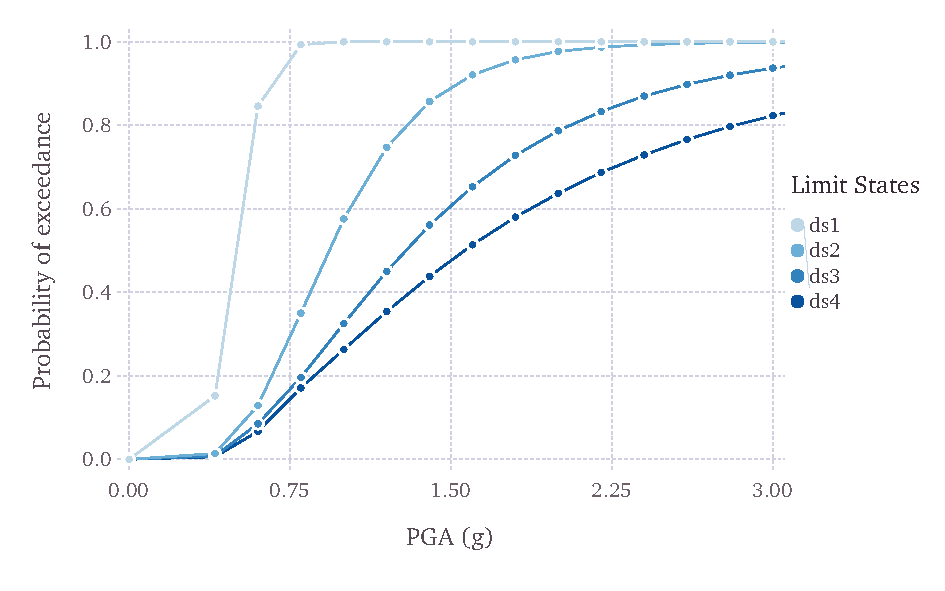
\includegraphics[width=12cm]{figures/risk/fragility-discrete.pdf}
\caption{Graphical representation of a discrete fragility model}
\label{fig:fragility-discrete}
\end{figure}

The \glspl{fragilityfunction} can also be defined as continuous functions,
through the use of cumulative lognormal distribution functions. In
Figure~\ref{fig:fragility-continuous}, a continuous \gls{fragilitymodel} is
presented.

\begin{figure}[ht]
\centering
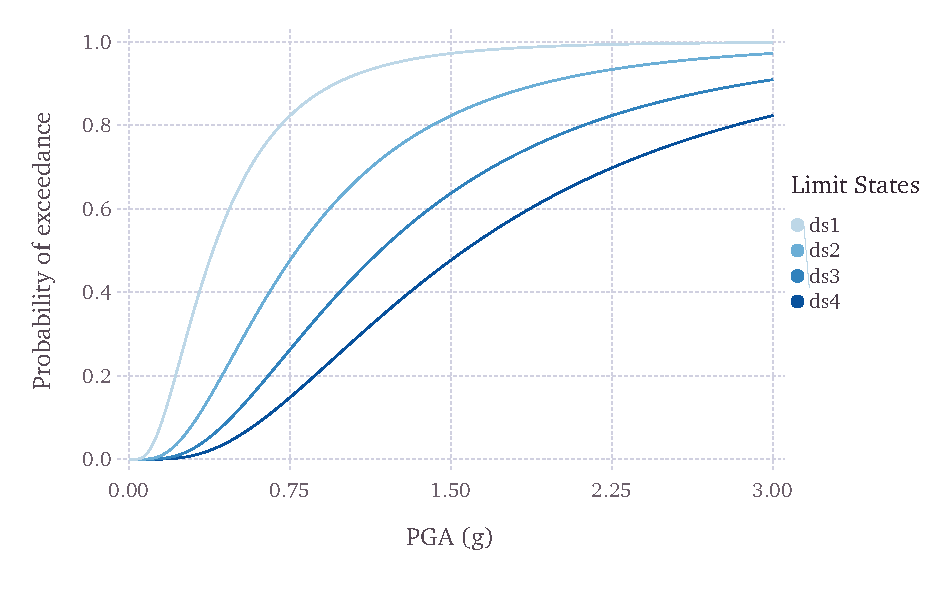
\includegraphics[width=12cm]{figures/risk/fragility-continuous.pdf}
\caption{Graphical representation of a continuous fragility model}
\label{fig:fragility-continuous}
\end{figure}

An example \gls{fragilitymodel} comprising one discrete
\gls{fragilityfunction} and one continuous \gls{fragilityfunction} is shown in
Listing~\ref{lst:input_fragility}.

\begin{listing}[htbp]
  \inputminted[firstline=1,firstnumber=1,fontsize=\footnotesize,frame=single,linenos,bgcolor=lightgray]{xml}{oqum/risk/Verbatim/input_fragility.xml}
  \caption{Example fragility model comprising one discrete fragility function and one continuous fragility function (\href{https://raw.githubusercontent.com/GEMScienceTools/oq-engine-docs/master/oqum/risk/verbatim/input_fragility.xml}{Download example})}
  \label{lst:input_fragility}
\end{listing}


The initial portion of the schema contains general information that describes
some general aspects of the \gls{fragilitymodel}. The information in this
metadata section is common to all of the functions in the \gls{fragilitymodel}
and needs to be included at the beginning of every \gls{fragilitymodel} file.
The parameters of the metadata section are shown in the snippet below and
described after the snippet:

\inputminted[firstline=4,firstnumber=4,lastline=9,fontsize=\footnotesize,frame=single,linenos,bgcolor=lightgray]{xml}{oqum/risk/Verbatim/input_fragility.xml}

\begin{itemize}

    \item \Verb+id+: mandatory; a unique string used to identify the 
      \gls{fragilitymodel}. This string can contain letters~(a--z; A--Z), 
      numbers~(0--9), dashes~(-), and underscores~(\_), with a maximum of 
      100~characters.

    \item \Verb+assetCategory+: an optional string used to specify the type of
      \glspl{asset} for which \glspl{fragilityfunction} will be defined in this
      file (e.g: buildings, lifelines).

    \item \Verb+lossCategory+: mandatory; valid strings for this attribute are 
      ``structural'', ``nonstructural'', ``contents'', and 
      ``business\_interruption''.

    \item \Verb+description+: mandatory; a brief string (ASCII) with further 
      relevant information about the \gls{fragilitymodel}, 
      for example, which building typologies are covered
      or the source of the functions in the \gls{fragilitymodel}.

    \item \Verb+limitStates+: mandatory; this field is used to define the number and 
      nomenclature of each limit state. Four limit states are employed in the 
      example above, but it is possible to use any number of discrete states,
      as long as a fragility curve is always defined for each limit state. The 
      limit states must be provided as a set of strings separated by whitespaces 
      between each limit state. Each limit state string can contain
      letters~(a--z; A--Z), numbers~(0--9), dashes~(-), and underscores~(\_).
      Please ensure that there is no whitespace within the name of any
      individual limit state.

\end{itemize}



The following snippet from the above \gls{fragilitymodel} example file defines a
discrete \gls{fragilityfunction}:

\inputminted[firstline=11,firstnumber=11,lastline=17,fontsize=\footnotesize,frame=single,linenos,bgcolor=lightgray]{xml}{oqum/risk/Verbatim/input_fragility.xml}

The following attributes are needed to define a discrete \gls{fragilityfunction}:

\begin{itemize}

    \item \Verb+id+: mandatory; a unique string used to identify the 
      \gls{taxonomy} for which the function is being defined. This string is
      used to relate the \gls{fragilityfunction} with the relevant \gls{asset}
      in the \gls{exposuremodel}. This string can contain letters~(a--z; A--Z),
      numbers~(0--9), dashes~(-), and underscores~(\_), with a maximum of
      100~characters.

    \item \Verb+format+: mandatory; for discrete \glspl{fragilityfunction}, this
      attribute should be set to ``\Verb+discrete+''.

    \item \Verb+imls+: mandatory; this attribute specifies the list of intensity levels
      for which the limit state probabilities of exceedance will be defined. 
      In addition, it is also necessary to define the intensity measure type 
      (\Verb+imt+). Optionally, a \Verb+noDamageLimit+ can be specified, which 
      defines the intensity level below which the probability of exceedance 
      for all limit states is taken to be zero.

    \item \Verb+poes+: mandatory; this field is used to define the probabilities of 
      exceedance (\Verb+poes+) for each limit state for each discrete 
      \gls{fragilityfunction}. It is also necessary to specify which limit 
      state the exceedance probabilities are being defined for using the 
      attribute \Verb+ls+. The probabilities of exceedance for each limit state
      must be provided on a separate line; and the number of exceedance 
      probabilities for each limit state defined by the \Verb+poes+ attribute 
      must be equal to the number of intensity levels defined by the attribute 
      \Verb+imls+. Finally, the number and names of the limit states in each 
      fragility function must be equal to the number of limit states defined 
      earlier in the metadata section of the \gls{fragilitymodel} using the 
      attribute \Verb+limitStates+.

\end{itemize}



The following snippet from the above \gls{fragilitymodel} example file
defines a continuous \gls{fragilityfunction}:

\inputminted[firstline=19,firstnumber=19,lastline=25,fontsize=\footnotesize,frame=single,linenos,bgcolor=lightgray]{xml}{oqum/risk/Verbatim/input_fragility.xml}

The following attributes are needed to define a continuous \gls{fragilityfunction}:

\begin{itemize}

    \item \Verb+id+: mandatory; a unique string used to identify the 
      \gls{taxonomy} for which the function is being defined. This string is
      used to relate the \gls{fragilityfunction} with the relevant \gls{asset}
      in the \gls{exposuremodel}. This string can contain letters~(a--z; A--Z),
      numbers~(0--9), dashes~(-), and underscores~(\_), with a maximum of
      100~characters.

    \item \Verb+format+: mandatory; for continuous \glspl{fragilityfunction},
      this attribute should be set to ``\Verb+continuous+''.

    \item \Verb+shape+: mandatory; for continuous \glspl{fragilityfunction}
      using the lognormal cumulative distrution, this attribute should be set
      to ``\Verb+logncdf+''. At present, only the lognormal cumulative
      distribution function can be used for representing continuous
      \glspl{fragilityfunction}.

    \item \Verb+imls+: mandatory; this element specifies aspects related to the
      intensity measure used by the the \gls{fragilityfunction}. The range of 
      intensity levels for which the continuous \glspl{fragilityfunction} are valid
      is specified using the attributes \Verb+minIML+ and \Verb+maxIML+. 
      In addition, it is also necessary to define the intensity measure type 
      \Verb+imt+. Optionally, a \Verb+noDamageLimit+ can be specified, which 
      defines the intensity level below which the probability of exceedance 
      for all limit states is taken to be zero.

    \item \Verb+params+: mandatory; this field is used to define the parameters
      of the continuous curve for each limit state for this 
      \gls{fragilityfunction}. For a lognormal cumulative distrbution function, 
      the two parameters required to specify the function are the mean and 
      standard deviation of the intensity level. These parameters are defined for 
      each limit state using the attributes \Verb+mean+ and \Verb+stddev+ 
      respectively. The attribute \Verb+ls+ specifies the limit state for which 
      the parameters are being defined. The parameters for each limit state
      must be provided on a separate line. The number and names of the limit 
      states in each \gls{fragilityfunction} must be equal to the number of limit 
      states defined earlier in the metadata section of the \gls{fragilitymodel}
      using the attribute \Verb+limitStates+.

\end{itemize}


Note that the schema for representing \glspl{fragilitymodel} has changed
between \gls{acr:nrml} v0.4 (used prior to \gls{acr:oqe17}) and \gls{acr:nrml}
v0.5 (introduced in \gls{acr:oqe17}).

A deprecation warning is printed every time you attempt to use a
\gls{fragilitymodel} in the old \gls{acr:nrml} v0.4 format in an
\gls{acr:oqe17} (or later) risk calculation. To get rid of the warning you
must upgrade the old \glspl{fragilitymodel} files to \gls{acr:nrml} v0.5. You
can use the command \Verb+upgrade_nrml+ with oq to do this as follows:

\begin{minted}[fontsize=\footnotesize,frame=single,bgcolor=lightgray]{shell-session}
user@ubuntu:~\$ oq upgrade_nrml <directory-name>
\end{minted}

The above command will upgrade all of your old \gls{fragilitymodel} files to
\gls{acr:nrml} v0.5. The original files will be kept, but with a .bak extension
appended. Notice that you will need to set the \Verb+lossCategory+ attribute
to its correct value manually. This is easy to do, since if you try to run a
computation you will get a clear error message telling the expected value for
the \Verb+lossCategory+ for each file.


Several methodologies to derive \glspl{fragilityfunction} are currently being
evaluated by \gls{acr:gem} and have been included as part of the Risk
Modeller's Toolkit, the code for which can be found on a public repository at
GitHub at the following address: 
\href{http://github.com/gemsciencetools/rmtk}{http://github.com/gemsciencetools/rmtk}.

A web-based tool to build a \gls{fragilitymodel} in the \gls{acr:nrml} schema
are also under development, and can be found at the OpenQuake platform at the
following address: \href{https://platform.openquake.org/ipt/}{https://platform.openquake.org/ipt/}.

\section{Consequence Models}
\label{sec:consequence}
Starting from \glsdesc{acr:oqe17}, the Scenario Damage calculator also accepts
\glspl{consequencemodel} in addition to \glspl{fragilitymodel}, in order to
estimate consequences based on the calculated damage distribution. The user
may provide one \gls{consequencemodel} file corresponding to each loss type
(amongst structural, nonstructural, contents, and business interruption) for
which a \gls{fragilitymodel} file is provided. Whereas providing a
\gls{fragilitymodel} file for at least one loss type is mandatory for running
a Scenario Damage calculation, providing corresponding \gls{consequencemodel}
files is optional.

This section describes the schema currently used to store
\glspl{consequencemodel}, which are optional inputs for the Scenario Damage
Calculator. A \gls{consequencemodel} defines a set of
\glspl{consequencefunction}, describing the distribution of the loss (or
consequence) ratio conditional on a set of discrete limit (or damage) states.
These \gls{consequencefunction} can be currently defined in \glsdesc{acr:oqe}
by specifying the parameters of the continuous distribution of the loss ratio
for each limit state specified in the fragility model for the corresponding
loss type, for each taxonomy defined in the exposure model.

An example \gls{consequencemodel} is shown in Listing~\ref{lst:input_consequence}.

\begin{listing}[htbp]
  \inputminted[firstline=1,firstnumber=1,fontsize=\footnotesize,frame=single,linenos,bgcolor=lightgray]{xml}{oqum/risk/verbatim/input_consequence.xml}
  \caption{Example consequence model (\href{https://raw.githubusercontent.com/gem/oq-engine/master/doc/manual/oqum/risk/verbatim/input_consequence.xml}{Download example})}
  \label{lst:input_consequence}
\end{listing}	

The initial portion of the schema contains general information that describes
some general aspects of the \gls{consequencemodel}. The information in this
metadata section is common to all of the functions in the
\gls{consequencemodel} and needs to be included at the beginning of every
\gls{consequencemodel} file. The parameters are described below:

\begin{itemize}

  \item \Verb+id+: a unique string used to identify the \gls{consequencemodel}.
    This string can contain letters~(a--z; A--Z), numbers~(0--9), dashes~(-), 
    and underscores~(\_), with a maximum of 100~characters.

  \item \Verb+assetCategory+: an optional string used to specify the type of
    \glspl{asset} for which \glspl{consequencefunction} will be defined in
    this file (e.g: buildings, lifelines).

  \item \Verb+lossCategory+: mandatory; valid strings for this attribute are 
    ``structural'', ``nonstructural'', ``contents'', and 
    ``business\_interruption''.

  \item \Verb+description+: mandatory; a brief string (ASCII) with further 
    information about the \gls{consequencemodel}, for example, which building
    typologies are covered or the source of the functions in the
    \gls{consequencemodel}.

  \item \Verb+limitStates+: mandatory; this field is used to define the number and 
    nomenclature of each limit state. Four limit states are employed in the 
    example above, but it is possible to use any number of discrete states. The 
    limit states must be provided as a set of strings separated by whitespaces 
    between each limit state. Each limit state string can contain
    letters~(a--z; A--Z), numbers~(0--9), dashes~(-), and underscores~(\_). 
    Please ensure that there is no whitespace within the name of any individual
    limit state. The number and nomenclature of the limit states used in the
    \gls{consequencemodel} should match those used in the corresponding
    \gls{fragilitymodel}.

\end{itemize}

\inputminted[firstline=4,firstnumber=4,lastline=9,fontsize=\footnotesize,frame=single,linenos,bgcolor=lightgray]{xml}{oqum/risk/verbatim/input_consequence.xml}

The following snippet from the above \gls{consequencemodel} example file
defines a \gls{consequencefunction} using a lognormal distribution to model
the uncertainty in the consequence ratio for each limit state:

\inputminted[firstline=11,firstnumber=11,lastline=16,fontsize=\footnotesize,frame=single,linenos,bgcolor=lightgray]{xml}{oqum/risk/verbatim/input_consequence.xml}

The following attributes are needed to define a \gls{consequencefunction}:

\begin{itemize}

  \item \Verb+id+: mandatory; a unique string used to identify the 
    \gls{taxonomy} for which the function is being defined. This string is used
    to relate the \gls{consequencefunction} with the relevant \gls{asset} in the 
    \gls{exposuremodel}. This string can contain letters~(a--z; A--Z),
    numbers~(0--9), dashes~(-), and underscores~(\_), with a maximum of
    100~characters.

  \item \Verb+dist+: mandatory; for vulnerability function which use a continuous 
    distribution to model the uncertainty in the conditional loss ratios, 
    this attribute should be set to either ``\Verb+LN+'' if using the lognormal
    distribution, or to ``\Verb+BT+'' if using the Beta distribution
    \footnote{Note that as of \glsdesc{acr:oqe18}, the uncertainty in the 
    consequence ratios is ignored, and only the mean consequence ratios for the
    set of limit states is considered when computing the consequences from the
    damage distribution. Consideration of the uncertainty in the consequence
    ratios is planned for future releases of the \glsdesc{acr:oqe}.}.

  \item \Verb+params+: mandatory; this field is used to define the parameters of 
    the continuous distribution used for modelling the uncertainty in the
    loss ratios for each limit state for this 
    \gls{consequencefunction}. For a lognormal distrbution, 
    the two parameters required to specify the function are the mean and 
    standard deviation of the consequence ratio. These parameters are defined for 
    each limit state using the attributes \Verb+mean+ and \Verb+stddev+ 
    respectively. The attribute \Verb+ls+ specifies the limit state for which 
    the parameters are being defined. The parameters for each limit state
    must be provided on a separate line. The number and names of the limit 
    states in each \gls{consequencefunction} must be equal to the number of limit 
    states defined in the corresponding \gls{fragilitymodel}
    using the attribute \Verb+limitStates+.

\end{itemize}

\section{Vulnerability Models}
\label{sec:vulnerability}
In order to perform probabilistic or scenario risk calculations, it is
necessary to define a \gls{vulnerabilityfunction} for each building typology
present in the \gls{exposuremodel}. In this section, the schema for the
\gls{vulnerabilitymodel} is described in detail. A graphical representation of
a \gls{vulnerabilitymodel} (mean loss ratio for a set of intensity measure
levels) is illustrated in Figure~\ref{fig:vulnerability-zero-cov}.

\begin{figure}[ht]
\centering
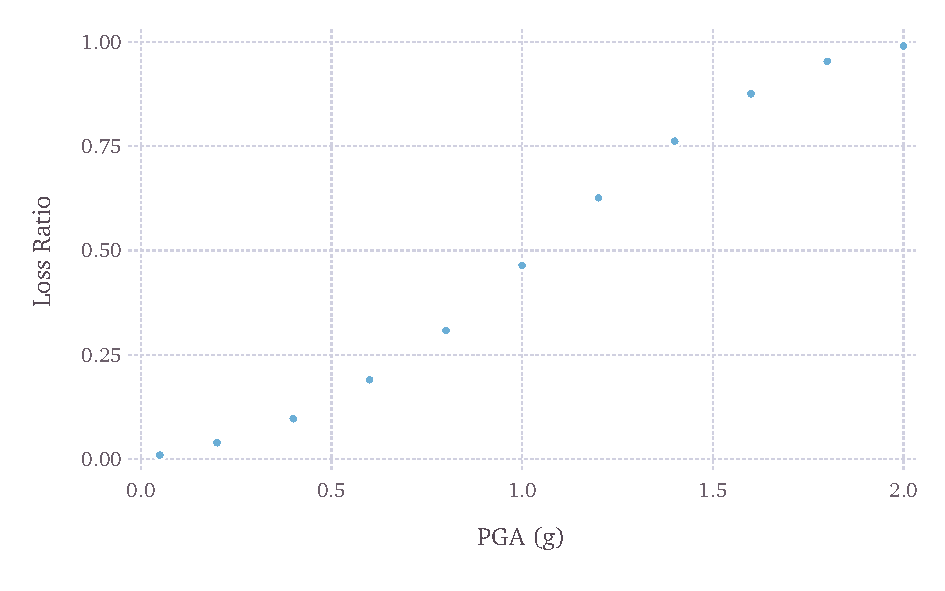
\includegraphics[width=12cm]{figures/risk/vulnerability-zero-cov.pdf}
\caption{Graphical representation of a vulnerability model}
\label{fig:vulnerability-zero-cov}
\end{figure}


Note that although the uncertainty for each loss ratio is not represented in
Figure~\ref{fig:vulnerability-zero-cov}, it can be considered in the input
file, by means of a coefficient of variation per loss ratio and a
probabilistic distribution, which can currently be set to lognormal~(LN),
Beta~(BT); or by specifying a discrete probability mass~(PM)\footnote{As of
\glsdesc{acr:oqe18}, the ``PM'' option for defining
\glspl{vulnerabilityfunction} is supported by the Scenario Risk and the
Stochastic Event-Based Probabilistic Risk Calculators, but not by the
Classical Probabilistic Risk Calculator.} distribution of the loss ratio at a
set of intensity levels. An example of a \gls{vulnerabilityfunction} that
models the uncertainty in the loss ratio at different intensity levels using a
lognormal distribution is illustrated in 
Figure~\ref{fig:vulnerability-nonzero-cov}.

\begin{figure}[ht]
\centering
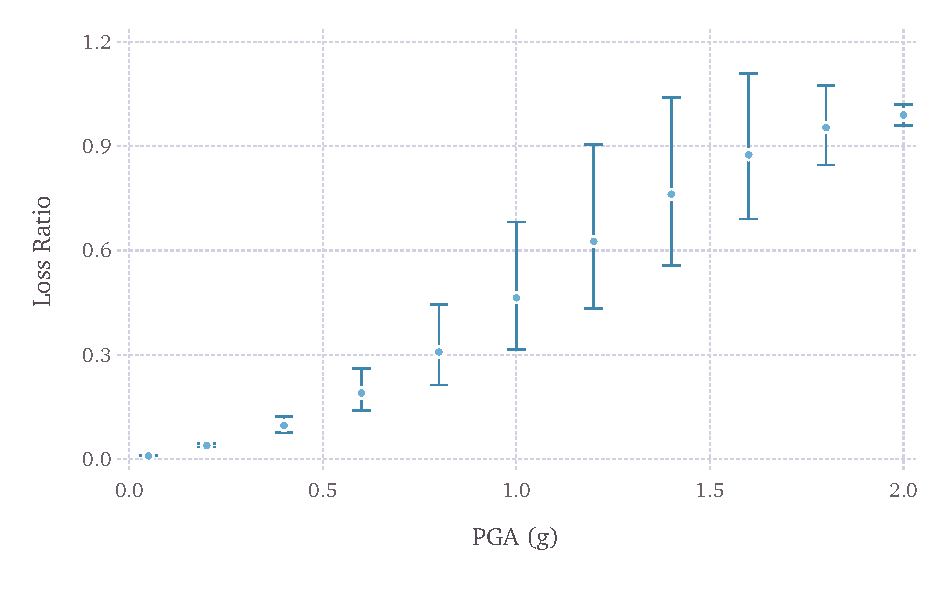
\includegraphics[width=12cm]{figures/risk/vulnerability-nonzero-cov.pdf}
\caption{Graphical representation of a vulnerability function that models the uncertainty in the loss ratio using a lognormal distribution. The mean loss ratios and coefficients of variation are illustrated for a set of intensity levels.}
\label{fig:vulnerability-nonzero-cov}
\end{figure}

In general, defining \glspl{vulnerabilityfunction} requires the user to
specify the distribution of the loss ratio for a set of intensity levels. The
loss ratio distributions can be defined using either a discrete or a
continuous format, and the \gls{vulnerabilitymodel} file can include a mix of
both types of \glspl{vulnerabilityfunction}. It is also possible to define a
\gls{vulnerabilityfunction} using a set of deterministic loss ratios
corresponding to a set of intensity levels (i.e., ignoring the uncertainty in
the conditional loss ratios).

An example \gls{vulnerabilitymodel} comprising three
\glspl{vulnerabilityfunction} is shown in
Listing~\ref{lst:input_vulnerability}. This \gls{vulnerabilitymodel} contains
one function that uses the lognormal distribution to represent the uncertainty
in the loss ratio at different intensity levels, one function that uses the
Beta distribution, and one function that is defined using a discrete
probability mass distribution.

\begin{listing}[htbp]
  \inputminted[firstline=1,firstnumber=1,fontsize=\footnotesize,frame=single,linenos,bgcolor=lightgray]{xml}{oqum/risk/verbatim/input_vulnerability.xml}
  \caption{Example vulnerability model (\href{https://raw.githubusercontent.com/gem/oq-engine/master/doc/manual/oqum/risk/verbatim/input_vulnerability.xml}{Download example})}
  \label{lst:input_vulnerability}
\end{listing}


The initial portion of the schema contains general information that describes
some general aspects of the \gls{vulnerabilitymodel}. The information in this
metadata section is common to all of the functions in the
\gls{vulnerabilitymodel} and needs to be included at the beginning of every
\gls{vulnerabilitymodel} file. The parameters are illustrated in the snippet
shown and described below:

\inputminted[firstline=4,firstnumber=4,lastline=8,fontsize=\footnotesize,frame=single,linenos,bgcolor=lightgray]{xml}{oqum/risk/verbatim/input_vulnerability.xml}

\begin{itemize}

  \item \Verb+id+: a unique string (ASCII) used to identify the
    \gls{vulnerabilitymodel}. This string can contain letters~(a--z; A--Z),
    numbers~(0--9), dashes~(-), and underscores~(\_), with a maximum of
    100~characters.

  \item \Verb+assetCategory+: an optional string (ASCII) used to specify the
    type of \glspl{asset} for which \glspl{vulnerabilityfunction} will be 
    defined in this file (e.g: buildings, lifelines).

  \item \Verb+lossCategory+: mandatory; valid strings for this attribute are 
    ``structural'', ``nonstructural'', ``contents'',  
    ``business\_interruption'', and ``occupants''.

  \item \Verb+description+: mandatory; a brief string with further information about the
    \gls{vulnerabilitymodel}, for example, which building typologies are 
    covered or the source of the functions in the \gls{vulnerabilitymodel}.

\end{itemize}


The following snippet from the above \gls{vulnerabilitymodel} example file defines
a \gls{vulnerabilityfunction} modelling the uncertainty in the conditional loss
ratios using a (continuous) lognormal distribution:

\inputminted[firstline=10,firstnumber=10,lastline=14,fontsize=\footnotesize,frame=single,linenos,bgcolor=lightgray]{xml}{oqum/risk/verbatim/input_vulnerability.xml}

The following attributes are needed to define a \gls{vulnerabilityfunction} which
uses a continuous distribution to model the uncertainty in the conditional
loss ratios:

\begin{itemize}

  \item \Verb+id+: a unique string (ASCII) used to identify the \gls{taxonomy} for 
    which the function is being defined. This string is used to relate the 
    \gls{vulnerabilityfunction} with the relevant \gls{asset} in the 
    \gls{exposuremodel}. This string can contain letters~(a--z; A--Z), 
    numbers~(0--9), dashes~(-), and underscores~(\_), with a maximum of
    100~characters.

  \item \Verb+dist+: mandatory; for \glspl{vulnerabilityfunction} which use a continuous 
    distribution to model the uncertainty in the conditional loss ratios, 
    this attribute should be set to either ``\Verb+LN+'' if using the lognormal
    distribution, or to ``\Verb+BT+'' if using the Beta distribution.

  \item \Verb+imls+: mandatory; this attribute specifies the list of intensity levels
    for which the parameters of the conditional loss ratio distributions will
    be defined. In addition, it is also necessary to define the intensity 
    measure type (\Verb+imt+).

  \item \Verb+meanLRs+: mandatory; this field is used to define the mean loss ratios
    for this \gls{vulnerabilityfunction} for each of the intensity levels
    defined by the attribute \Verb+imls+. The number of mean loss ratios
    defined by the \Verb+meanLRs+ attribute must be equal to the number of
    intensity levels defined by the attribute \Verb+imls+.

  \item \Verb+covLRs+: mandatory; this field is used to define the coefficient of 
    variation for the conditional distribution of the loss ratios for this
    \gls{vulnerabilityfunction} for each of the intensity levels defined by
    the attribute \Verb+imls+. The number of coefficients of variation of loss
    ratios defined by the \Verb+covLRs+ attribute must be equal to the number
    of intensity levels defined by the attribute \Verb+imls+. The uncertainty
    in the conditional loss ratios can be ignored by setting all of the
    \Verb+covLRs+ for a given \gls{vulnerabilityfunction} to zero.

\end{itemize}


The next snippet from the \gls{vulnerabilitymodel} example file of
Listing~\ref{lst:input_vulnerability} defines a \gls{vulnerabilityfunction}
which models the uncertainty in the conditional loss ratios using a
(discrete) probability mass distribution:

\inputminted[firstline=24,firstnumber=24,lastline=33,fontsize=\footnotesize,frame=single,linenos,bgcolor=lightgray]{xml}{oqum/risk/verbatim/input_vulnerability.xml}

The following attributes are needed to define a \gls{vulnerabilityfunction}
which uses a discrete probability mass distribution to model the uncertainty
in the conditional loss ratios:

\begin{itemize}

  \item \Verb+id+: a unique string (ASCII) used to identify the \gls{taxonomy} for 
    which the function is being defined. This string is used to relate the 
    \gls{vulnerabilityfunction} with the relevant \gls{asset} in the 
    \gls{exposuremodel}. This string can contain letters~(a--z; A--Z), 
    numbers~(0--9), dashes~(-), and underscores~(\_), with a maximum of
    100~characters.

  \item \Verb+dist+: mandatory; for \glspl{vulnerabilityfunction} which use a 
    discrete probability mass distribution to model the uncertainty in the
    conditional loss ratios, this attribute should be set to ``\Verb+PM+''.

  \item \Verb+imls+: mandatory; this attribute specifies the list of intensity levels
    for which the parameters of the conditional loss ratio distributions will
    be defined. In addition, it is also necessary to define the intensity 
    measure type (\Verb+imt+).

  \item \Verb+probabilities+: mandatory; this field is used to define the
    probability of observing a particular loss ratio (specified for each row of
    \Verb+probabilities+ using the attribute \Verb+lr+), conditional on the set
    of intensity levels specified using the attribute \Verb+imls+.
    for this \gls{vulnerabilityfunction}. Thus, the number of probabilities
    defined by each \Verb+probabilities+ attribute must be equal to the number
    of intensity levels defined by the attribute \Verb+imls+. On the other hand,
    there is no limit to the number of loss ratios for which
    \Verb+probabilities+ can be defined. In the example shown here, notice that
    the set of probabilities conditional on any particular intensity level,
    say, $MMI = 8$, sum up to one.

\end{itemize}


Note that the schema for representing \glspl{vulnerabilitymodel} has changed
between \gls{acr:nrml} v0.4 (used prior to \gls{acr:oqe17}) and \gls{acr:nrml}
v0.5 (introduced in \gls{acr:oqe17}).

A deprecation warning is printed every time you attempt to use a
\gls{vulnerabilitymodel} in the old \gls{acr:nrml} v0.4 format in an
\gls{acr:oqe17} (or later) risk calculation. To get rid of the warning you
must upgrade the old \glspl{vulnerabilitymodel} files to \gls{acr:nrml} v0.5.
You can use the command \Verb+upgrade_nrml+ with oq to do this as
follows:

\begin{minted}[fontsize=\footnotesize,frame=single,bgcolor=lightgray]{shell-session}
user@ubuntu:~\$ oq upgrade_nrml <directory-name>
\end{minted}

The above command will upgrade all of your old \gls{vulnerabilitymodel} files to
\gls{acr:nrml} v0.5. The original files will be kept, but with a .bak extension
appended. Notice that you will need to set the \Verb+lossCategory+ attribute
to its correct value manually. This is easy to do, since if you try to run a
computation you will get a clear error message telling the expected value for
the \Verb+lossCategory+ for each file.


Several methodologies to derive \glspl{vulnerabilityfunction} are currently being
evaluated by \gls{acr:gem} and have been included as part of the Risk
Modeller's Toolkit, the code for which can be found on a public repository at
GitHub at: 
\href{http://github.com/gemsciencetools/rmtk}{http://github.com/gemsciencetools/rmtk}.

A web-based tool to build an \gls{vulnerabilitymodel} in the \gls{acr:nrml} schema
are also under development, and can be found at the OpenQuake platform at the
following address: \href{https://platform.openquake.org/ipt/}{https://platform.openquake.org/ipt/}.

   \cleardoublepage

\chapterimage{figures/chapter_head.pdf} % Chapter heading image
\chapter{Using the Risk Module}
	\label{chap:riskcalculators}
	This Chapter summarises the structure of the information necessary to define
the different input data to be used with the \glsdesc{acr:oqe} risk
calculators. Input data for scenario-based and probabilistic seismic damage
and risk analysis using the \glsdesc{acr:oqe} are organised into:

\begin{itemize}

  \item An exposure model file in the NRML format, as described in 
    Section~\ref{sec:exposure}.

  \item A file describing the \gls{vulnerabilitymodel}
    (Section~\ref{sec:vulnerability}) for loss calculations, or a 
  	file describing the \gls{fragilitymodel} (Section~\ref{sec:fragility})
    for damage calculations. Optionally, a file describing the
    \gls{consequencemodel} (Section~\ref{sec:consequence}) can also be
  	provided in order to calculate losses from the estimated damage
  	distributions.

  \item A general calculation configuration file.

  \item Hazard inputs. These include hazard curves for the classical
    probabilistic damage and risk calculators, ground motion fields for the
    scenario damage and risk calculators, or stochastic event sets for the
    probabilistic event based calculators. As of \glsdesc{acr:oqe21}, in
    general, there are five different ways in which hazard calculation
    parameters or results can be provided to the \glsdesc{acr:oqe} in order to
    run the subsequent risk calculations:

    \begin{itemize}

      \item Use a single configuration file for running the hazard and risk
      calculations sequentially (preferred)

      \item Use separate configuration files for running the hazard and risk
      calculations sequentially (legacy)

      \item Use a configuration file for the risk calculation along with all
      hazard outputs from a previously completed, compatible
      \glsdesc{acr:oqe} hazard calculation

      % \item Use a configuration file for the risk calculation along with a
      % specific hazard output from a previously completed, compatible
      % \glsdesc{acr:oqe} hazard calculation

      \item Use a configuration file for the risk calculation along with
      hazard input files in the OpenQuake NRML format

    \end{itemize}

\end{itemize}

The file formats for \glspl{exposuremodel}, \glspl{fragilitymodel},
\glspl{consequencemodel}, and \glspl{vulnerabilitymodel} have been described
earlier in Chapter~\ref{chap:riskinputs}. The configuration file is the primary
file that provides the \glsdesc{acr:oqe} information regarding both the
definition of the input models (e.g. exposure, site parameters, fragility,
consequence, or vulnerability models) as well as the parameters governing the
risk calculation.

Information regarding the configuration file for running hazard calculations
using the \glsdesc{acr:oqe} can be found in
Section~\ref{sec:hazard_configuration_file}. Some initial mandatory parameters
of the configuration file common to all of the risk calculators are presented
in Listing~\ref{lst:config_example}. The remaining parameters that are
specific to each risk calculator are discussed in subsequent sections.

\begin{listing}[htbp]
  \inputminted[firstline=1,firstnumber=1,fontsize=\footnotesize,frame=single,linenos,bgcolor=lightgray]{ini}{oqum/risk/verbatim/config_example.ini}
  \caption{Example minimal risk calculation configuration file (\href{https://raw.githubusercontent.com/gem/oq-engine/master/doc/manual/oqum/risk/verbatim/config_example.xml}{Download example})}
  \label{lst:config_example}
\end{listing}

\begin{itemize}

  \item \Verb+description+: a parameter that can be used to include some
  information about the type of calculations that are going to be performed.

  \item \Verb+calculation_mode+: this parameter specifies the type of
  calculation to be run. Valid options for the \Verb+calculation_mode+ for
  the risk calculators are: \Verb+scenario_damage+, \Verb+scenario_risk+,
  \Verb+classical_damage+, \Verb+classical_risk+, \Verb+event_based_risk+,
  and \Verb+classical_bcr+.

  \item \Verb+exposure_file+: this parameter is used to specify the path to
  the \gls{exposuremodel} file.

\end{itemize}

Depending on the type of risk calculation, other parameters besides the
aforementioned ones may need to be provided. We illustrate in the following
sections different examples of the configuration file for the different risk
calculators.


\section{Scenario Damage Calculator}
\label{sec:config_scenario_damage}
For this calculator, the parameter \Verb+calculation_mode+ should be set to
\Verb+scenario_damage+.

\paragraph{Example 1}

This example illustrates a scenario damage calculation which uses a single
configuration file to first compute the ground motion fields for the given
rupture model and then calculate damage distribution statistics based on the
ground motion fields. A minimal job configuration file required for running a
scenario damage calculation is shown in
Listing~\ref{lst:config_scenario_damage_combined}.

\begin{listing}[htbp]
  \inputminted[firstline=1,firstnumber=1,fontsize=\footnotesize,frame=single,linenos,bgcolor=lightgray,label=job.ini]{ini}{oqum/risk/verbatim/config_scenario_damage_combined.ini}
  \caption{Example combined configuration file for running a scenario damage calculation (\href{https://raw.githubusercontent.com/gem/oq-engine/master/doc/manual/oqum/risk/verbatim/config_scenario_damage_combined.ini}{Download example})}
  \label{lst:config_scenario_damage_combined}
\end{listing}

The general parameters \Verb+description+ and \Verb+calculation_mode+, and
\Verb+exposure_file+ have already been described earlier. The other parameters
seen in the above example configuration file are described below:

\begin{itemize}

  \item \Verb+rupture_model_file+: a parameter used to define the path
	to the earthquake \gls{rupturemodel} file describing the scenario event.

  \item \Verb+rupture_mesh_spacing+: a parameter used to specify the mesh size
  	(in km) used by the \glsdesc{acr:oqe} to discretize the rupture.
  	Note that the smaller the mesh spacing, the greater will be
  	(1) the precision in the calculation and
  	(2) the computational demand.

  \item \Verb+structural_fragility_file+: a parameter used to define the path
	to the structural \gls{fragilitymodel} file.

\end{itemize}

In this case, the ground motion fields will be computed at each of the
locations of the assets in the exposure model. Ground motion fields will be
generated for each of the intensity measure types found in the provided set of
fragility models. The above calculation can be run using the command line:

\begin{minted}[fontsize=\footnotesize,frame=single,bgcolor=lightgray]{shell-session}
user@ubuntu:~\$ oq engine --run job.ini
\end{minted}

After the calculation is completed, a message similar to the following will be
displayed:

\begin{minted}[fontsize=\footnotesize,frame=single,bgcolor=lightgray]{shell-session}
Calculation 2680 completed in 13 seconds. Results:
  id | name
5069 | Average Asset Damages
\end{minted}

Note that one or more of the following parameters can be used in the same job
configuration file to provide the corresponding fragility model files:

\begin{itemize}

  \item \Verb+structural_fragility_file+: a parameter used to define the path
    to a structural \gls{fragilitymodel} file

  \item \Verb+nonstructural_fragility_file+: a parameter used to define the path
    to a nonstructural \gls{fragilitymodel} file

  \item \Verb+contents_fragility_file+: a parameter used to define the path
    to a contents \gls{fragilitymodel} file

  \item \Verb+business_interruption_fragility_file+: a parameter used to define
    the path to a business interruption \gls{fragilitymodel} file

\end{itemize}

It is important that the \Verb+lossCategory+ parameter in the metadata section
for each provided fragility model file (``structural'', ``nonstructural'',
``contents'', or ``business\_interruption'') should match the loss type
defined in the configuration file by the relevant keyword above.


\paragraph{Example 2}

This example illustrates a scenario damage calculation which uses separate
configuration files for the hazard and risk parts of a scenario damage
assessment. The first configuration file shown in
Listing~\ref{lst:config_scenario_damage_hazard} contains input models and
parameters required for the computation of the ground motion fields due to a
given rupture. The second configuration file shown in
Listing~\ref{lst:config_scenario_damage} contains input models and parameters
required for the calculation of the damage distribution for a portfolio of
assets due to the ground motion fields.

\begin{listing}[htbp]
  \inputminted[firstline=1,firstnumber=1,fontsize=\footnotesize,frame=single,linenos,bgcolor=lightgray,label=job\_hazard.ini]{ini}{oqum/risk/verbatim/config_scenario_hazard.ini}
  \caption{Example hazard configuration file for a scenario damage calculation (\href{https://raw.githubusercontent.com/gem/oq-engine/master/doc/manual/oqum/risk/verbatim/config_scenario_hazard.ini}{Download example})}
  \label{lst:config_scenario_damage_hazard}
\end{listing}

\begin{listing}[htbp]
  \inputminted[firstline=1,firstnumber=1,fontsize=\footnotesize,frame=single,linenos,bgcolor=lightgray,label=job\_damage.ini]{ini}{oqum/risk/verbatim/config_scenario_damage.ini}
  \caption{Example risk configuration file for a scenario damage calculation (\href{https://raw.githubusercontent.com/gem/oq-engine/master/doc/manual/oqum/risk/verbatim/config_scenario_damage.ini}{Download example})}
  \label{lst:config_scenario_damage}
\end{listing}


In this example, the set of intensity measure types for which the ground
motion fields should be generated is specified explicitly in the configuration
file using the parameter \Verb+intensity_measure_types+. If the hazard
calculation outputs are intended to be used as inputs for a subsequent
scenario damage or risk calculation, the set of intensity measure types
specified here must include all intensity measure types that are used in the
fragility or vulnerability models for the subsequent damage or risk
calculation.

In the hazard configuration file illustrated above
(Listing~\ref{lst:config_scenario_damage_hazard}), the list of sites at which
the ground motion values will be computed is provided in a CSV file, specified
using the \Verb+sites_csv+ parameter. The sites used for the hazard
calculation need not be the same as the locations of the assets in the
exposure model used for the following risk calculation. In such cases, it is
recommended to set a reasonable search radius (in km) using the
\Verb+asset_hazard_distance+ parameter for the \glsdesc{acr:oqe} to look for
available hazard values, as shown in the job\_damage.ini example file above.

The only new parameters introduced in risk configuration file for this example
(Listing~\ref{lst:config_scenario_damage}) are the \Verb+region_constraint+,
\Verb+asset_hazard_distance+, and \Verb+time_event+ parameters, which are
described below; all other parameters have already been described in earlier
examples.

\begin{itemize}

  \item \Verb+region_constraint+: this is an optional parameter, applicable
    only to risk calculations, which defines the polygon that will be used for
    filtering the assets from the exposure model. Assets outside of this region
    will not be considered in the risk calculations. This region is defined
    using pairs of coordinates that indicate the vertices of the polygon, which
    should be listed in the Well-known text (WKT) format:

    region\_constraint = lon\_1 lat\_1, lon\_2 lat\_2, ..., lon\_n lat\_n

    For each point, the longitude is listed first, followed by the latitude,
    both in decimal degrees. The list of points defining the polygon can be
    provided either in a clockwise or counter-clockwise direction.

    If the \Verb+region_constraint+ is not provided, all assets in the exposure
    model are considered for the risk calculation.

    This parameter is useful in cases where the exposure model covers a region
    larger than the one that is of interest in the current calculation.

  \item \Verb+asset_hazard_distance+: this parameter indicates the maximum
    allowable distance between an \gls{asset} and the closest hazard input.
    Hazard inputs can include hazard curves or ground motion intensity values.
    If no hazard input site is found within the radius defined by the
    \Verb+asset_hazard_distance+, the asset is skipped and a message is
    provided mentioning the id of the asset that is affected by this issue.

    If multiple hazard input sites are found within the radius defined by the
    this parameter, the hazard input site with the shortest distance from the
    asset location is associated with the asset. It is possible that the
    associated hazard input site might be located outside the polygon defined
    by the \Verb+region_constraint+.

  \item \Verb+time_event+: this parameter indicates the time of day at which
    the event occurs. The values that this parameter can be set to are 
    currently limited to one of the three strings: \Verb+day+, \Verb+night+,
    and \Verb+transit+. This parameter will be used to compute the number of
    fatalities based on the number of occupants present in the various
    \glspl{asset} at that time of day, as specified in the exposure model.

\end{itemize}


Now, the above calculations described by the two configuration files
``job\_hazard.ini'' and ``job\_damage.ini'' can be run separately. The
calculation id for the hazard calculation should be
provided to the \glsdesc{acr:oqe} while running the risk calculation using the
option \Verb+--hazard-calculation-id+ (or \Verb+--hc+). This is shown below:

\begin{minted}[fontsize=\footnotesize,frame=single,bgcolor=lightgray]{shell-session}
user@ubuntu:~\$ oq engine --run job_hazard.ini
\end{minted}

After the hazard calculation is completed, a message similar to the one below
will be displayed in the terminal:

\begin{minted}[fontsize=\footnotesize,frame=single,bgcolor=lightgray]{shell-session}
Calculation 2681 completed in 4 seconds. Results:
  id | name
5072 | Ground Motion Fields
\end{minted}

In the example above, the calculation~id of the hazard calculation is 2681.
There is only one output from this calculation, i.e., the \glspl{acr:gmf}.

The risk calculation for computing the damage distribution statistics for the
portfolio of \glspl{asset} can now be run using:

\begin{minted}[fontsize=\footnotesize,frame=single,bgcolor=lightgray]{shell-session}
user@ubuntu:~\$ oq engine --run job_damage.ini --hc 2681
\end{minted}

After the calculation is completed, a message similar to the one listed above
in Example~1 will be displayed.

In order to retrieve the calculation~id of a previously run hazard calculation,
the option \Verb+--list-hazard-calculations+ (or \Verb+--lhc+) can be used to
display a list of all previously run hazard calculations:

\begin{minted}[fontsize=\footnotesize,frame=single,bgcolor=lightgray]{shell-session}
job_id |     status |         start_time |         description
  2609 | successful | 2015-12-01 14:14:14 | Mid Nepal earthquake
  ...
  2681 | successful | 2015-12-12 10:00:00 | Scenario hazard example
\end{minted}

The option \Verb+--list-outputs+ (or \Verb+--lo+) can be used to display a
list of all outputs generated during a particular calculation. For instance,

\begin{minted}[fontsize=\footnotesize,frame=single,bgcolor=lightgray]{shell-session}
user@ubuntu:~\$ oq engine --lo 2681
\end{minted}

will produce the following display:

\begin{minted}[fontsize=\footnotesize,frame=single,bgcolor=lightgray]{shell-session}
  id | name
5072 | Ground Motion Fields
\end{minted}


\paragraph{Example 3}

The example shown in Listing~\ref{lst:config_scenario_damage_gmf_xml} illustrates
a scenario damage calculation which uses a file listing a precomputed set of
\glspl{acr:gmf}. These \glspl{acr:gmf} can be computed using the
\glsdesc{acr:oqe} or some other software. The \glspl{acr:gmf} must be provided
in either the \gls{acr:nrml} schema or the csv format as presented in
Section~\ref{subsec:output_scenario_hazard}. The damage distribution is
computed based on the provided \glspl{acr:gmf}.
Listing~\ref{lst:output_gmf_scenario_xml} shows an example of a
\glspl{acr:gmf} file in the \gls{acr:nrml} schema and
Table~\ref{output:gmf_scenario} shows an example of a \glspl{acr:gmf} file in
the csv format. If the \glspl{acr:gmf} file is provided in the csv format, an
additional csv file listing the site ids must be provided using the parameter
\Verb+sites_csv+. See Table~\ref{output:sitemesh} for an example of the sites
csv file, which provides the association between the site ids in the
\glspl{acr:gmf} csv file with their latitude and longitude coordinates.

\begin{listing}[htbp]
  \inputminted[firstline=1,firstnumber=1,fontsize=\footnotesize,frame=single,linenos,bgcolor=lightgray,label=job.ini]{ini}{oqum/risk/verbatim/config_scenario_damage_gmf_xml.ini}
  \caption{Example configuration file for a scenario damage calculation using a precomputed set of ground motion fields (\href{https://raw.githubusercontent.com/gem/oq-engine/master/doc/manual/oqum/risk/verbatim/config_scenario_damage_gmf_xml.ini}{Download example})}
  \label{lst:config_scenario_damage_gmf_xml}
\end{listing}

\begin{itemize}

  \item \Verb+gmfs_file+: a parameter used to define the path
    to the \glspl{acr:gmf} file in the \gls{acr:nrml} schema. This file must
    define \glspl{acr:gmf} for all of the intensity measure types used in the
    \gls{fragilitymodel}.

\end{itemize}

\begin{listing}[htbp]
  \inputminted[firstline=1,firstnumber=1,fontsize=\footnotesize,frame=single,linenos,bgcolor=lightgray,label=job.ini]{ini}{oqum/risk/verbatim/config_scenario_damage_gmf_csv.ini}
  \caption{Example configuration file for a scenario damage calculation using a precomputed set of ground motion fields (\href{https://raw.githubusercontent.com/gem/oq-engine/master/doc/manual/oqum/risk/verbatim/config_scenario_damage_gmf_csv.ini}{Download example})}
  \label{lst:config_scenario_damage_gmf_csv}
\end{listing}

\begin{itemize}

  \item \Verb+gmfs_csv+: a parameter used to define the path
    to the \glspl{acr:gmf} file in the csv format. This file must
    define \glspl{acr:gmf} for all of the intensity measure types used in the
    \gls{fragilitymodel}.
    (\href{https://raw.githubusercontent.com/gem/oq-engine/master/doc/manual/oqum/risk/verbatim/input_scenario_gmfs.csv}{Download an example file here}).

  \item \Verb+sites_csv+: a parameter used to define the path
    to the sites file in the csv format. This file must
    define site id, longitude, and latitude for all of the sites for the
    \glspl{acr:gmf} file provided using the \Verb+gmfs_csv+ parameter. 
    (\href{https://raw.githubusercontent.com/gem/oq-engine/master/doc/manual/oqum/risk/verbatim/input_scenario_sites.csv}{Download an example file here}).

\end{itemize}

The above calculation(s) can be run using the command line:

\begin{minted}[fontsize=\footnotesize,frame=single,bgcolor=lightgray]{shell-session}
user@ubuntu:~\$ oq engine --run job.ini
\end{minted}


\paragraph{Example 4}

This example illustrates a the hazard job configuration file for a scenario
damage calculation which uses two \glspl{acr:gmpe} instead of only one.
Currently, the set of \glspl{acr:gmpe} to be used for a scenario calculation
can be specified using a logic tree file, as demonstrated in
\ref{subsec:gmlt}. As of \glsdesc{acr:oqe18}, the weights in the logic tree
are ignored, and a set of \glspl{acr:gmf} will be generated for each
\gls{acr:gmpe} in the logic tree file. Correspondingly, damage distribution
statistics will be generated for each set of \gls{acr:gmf}.

The file shown in Listing~\ref{lst:input_scenario_gmlt} lists the two
\glspl{acr:gmpe} to be used for the hazard calculation:

\begin{listing}[htbp]
  \inputminted[firstline=1,firstnumber=1,fontsize=\footnotesize,frame=single,linenos,bgcolor=lightgray,label=gsim\_logic\_tree.xml]{xml}{oqum/risk/verbatim/input_scenario_gmlt.xml}
  \caption{Example ground motion logic tree for a scenario calculation (\href{https://raw.githubusercontent.com/gem/oq-engine/master/doc/manual/oqum/risk/verbatim/input_scenario_gmlt.xml}{Download example})}
  \label{lst:input_scenario_gmlt}
\end{listing}

The only change that needs to be made in the hazard job configuration file is
to replace the \Verb+gsim+ parameter with \Verb+gsim_logic_tree_file+, as
demonstrated in Listing~\ref{lst:config_scenario_hazard_gmlt}.

\begin{listing}[htbp]
  \inputminted[firstline=1,firstnumber=1,fontsize=\footnotesize,frame=single,linenos,bgcolor=lightgray,label=job\_hazard.ini]{ini}{oqum/risk/verbatim/config_scenario_hazard_gmlt.ini}
  \caption{Example configuration file for a scenario damage calculation using a logic-tree file (\href{https://raw.githubusercontent.com/gem/oq-engine/master/doc/manual/oqum/risk/verbatim/config_scenario_hazard_gmlt.ini}{Download example})}
  \label{lst:config_scenario_hazard_gmlt}
\end{listing}


\paragraph{Example 5}

This example illustrates a scenario damage calculation which specifies
fragility models for calculating damage to structural and nonstructural
components of structures, and also specifies \gls{consequencemodel} files for
calculation of the corresponding losses.

A minimal job configuration file required for running a scenario damage
calculation followed by a consequences analysis is shown in
Listing~\ref{lst:config_scenario_damage_consequences}.

\begin{listing}[htbp]
  \inputminted[firstline=1,firstnumber=1,fontsize=\footnotesize,frame=single,linenos,bgcolor=lightgray,label=job.ini]{ini}{oqum/risk/verbatim/config_scenario_damage_consequences.ini}
  \caption{Example configuration file for a scenario damage calculation followed by a consequences analysis (\href{https://raw.githubusercontent.com/gem/oq-engine/master/doc/manual/oqum/risk/verbatim/config_scenario_damage_consequences.ini}{Download example})}
  \label{lst:config_scenario_damage_consequences}
\end{listing}

Note that one or more of the following parameters can be used in the same job
configuration file to provide the corresponding \gls{consequencemodel} files:

\begin{itemize}

  \item \Verb+structural_consequence_file+: a parameter used to define the path
    to a structural \gls{consequencemodel} file

  \item \Verb+nonstructural_consequence_file+: a parameter used to define the path
    to a nonstructural \gls{consequencemodel} file

  \item \Verb+contents_consequence_file+: a parameter used to define the path
    to a contents \gls{consequencemodel} file

  \item \Verb+business_interruption_consequence_file+: a parameter used to define
    the path to a business interruption \gls{consequencemodel} file

\end{itemize}

It is important that the \Verb+lossCategory+ parameter in the metadata section
for each provided \gls{consequencemodel} file (``structural'', ``nonstructural'',
``contents'', or ``business\_interruption'') should match the loss type
defined in the configuration file by the relevant keyword above.

The above calculation can be run using the command line:

\begin{minted}[fontsize=\footnotesize,frame=single,bgcolor=lightgray]{shell-session}
user@ubuntu:~\$ oq engine --run job.ini
\end{minted}

After the calculation is completed, a message similar to the following will be
displayed:

\begin{minted}[fontsize=\footnotesize,frame=single,bgcolor=lightgray]{shell-session}
Calculation 1579 completed in 37 seconds. Results:
  id | name
8990 | Average Asset Losses
8993 | Average Asset Damages
\end{minted}


\section{Scenario Risk Calculator}
\label{sec:config_scenario_risk}
In order to run this calculator, the parameter \Verb+calculation_mode+ needs
to be set to \Verb+scenario_risk+. 

Most of the job configuration parameters required for running a scenario risk
calculation are the same as those described in the previous section for the
scenario damage calculator. The remaining parameters specific to the scenario
risk calculator are illustrated through the examples below.


\paragraph{Example 1}

This example illustrates a scenario risk calculation which uses a single
configuration file to first compute the ground motion fields for the given
rupture model and then calculate loss statistics for structural losses,
nonstructural losses, and insured structural losses, based on the ground
motion fields. The job configuration file required for running this scenario
risk calculation is shown in Listing~\ref{lst:config_scenario_risk_combined}.

\begin{listing}[htbp]
  \inputminted[firstline=1,firstnumber=1,fontsize=\footnotesize,frame=single,linenos,bgcolor=lightgray,label=job.ini]{ini}{oqum/risk/verbatim/config_scenario_risk_combined.ini}
  \caption{Example combined configuration file for a scenario risk calculation (\href{https://raw.githubusercontent.com/GEMScienceTools/oq-engine-docs/master/oqum/risk/verbatim/config_scenario_risk_combined.ini}{Download example})}
  \label{lst:config_scenario_risk_combined}
\end{listing}

Whereas a scenario damage calculation requires one or more fragility and/or
consequence models, a scenario risk calculation requires the user to specify
one or more vulnerability model files. Note that one or more of the following
parameters can be used in the same job configuration file to provide the
corresponding vulnerability model files:

\begin{itemize}

  \item \Verb+structural_vulnerability_file+: this parameter is used to
    specify the path to the structural \gls{vulnerabilitymodel} file

  \item \Verb+nonstructural_vulnerability_file+: this parameter is used to
    specify the path to the nonstructural\gls{vulnerabilitymodel} file

  \item \Verb+contents_vulnerability_file+: this parameter is used to
    specify the path to the contents \gls{vulnerabilitymodel} file

  \item \Verb+business_interruption_vulnerability_file+: this parameter is
    used to specify the path to the business interruption
    \gls{vulnerabilitymodel} file

  \item \Verb+occupants_vulnerability_file+: this parameter is used to
    specify the path to the occupants \gls{vulnerabilitymodel} file

\end{itemize}

It is important that the \Verb+lossCategory+ parameter in the metadata section
for each provided vulnerability model file (``structural'', ``nonstructural'',
``contents'', ``business\_interruption'', or ``occupants'') should match the
loss type defined in the configuration file by the relevant keyword above.

The remaining new parameters introduced in this example are the following:

\begin{itemize}

  \item \Verb+master_seed+: this parameter is used to control the random
    number generator in the loss ratio sampling process. If the same
    \Verb+master_seed+ is defined at each calculation run, the same random loss
    ratios will be generated, thus allowing reproducibility of the results.

  \item \Verb+asset_correlation+: if the uncertainty in the loss ratios
    has been defined within the \gls{vulnerabilitymodel}, users can specify
    a coefficient of correlation that will be used in the Monte Carlo sampling
    process of the loss ratios, between the assets that share the same
    \gls{taxonomy}. If the \Verb+asset_correlation+ is set to one,
    the loss ratio residuals will be perfectly correlated. On the other hand,
    if this parameter is set to zero, the loss ratios will be sampled
    independently. If this parameter is not defined, the
    \glsdesc{acr:oqe} will assume zero correlation in the vulnerability. As of
    \glsdesc{acr:oqe18}, \Verb+asset_correlation+ applies only to continuous
    \glspl{vulnerabilityfunction} using the lognormal or Beta distribution; 
    it does not apply to \glspl{vulnerabilityfunction} defined using the PMF
    distribution. Although partial correlation was supported in previous
    versions of the engine, beginning from \glsdesc{acr:oqe22}, values between
    zero and one are no longer supported due to performance considerations. The
    only two values permitted are \Verb+asset_correlation = 0+ and 
    \Verb+asset_correlation = 1+.

  \item \Verb+insured_losses+: this parameter specifies whether insured losses
    should be calculated; the default value of this parameter is \Verb+false+.
    In order for the \glsdesc{acr:oqe} to be able to compute insured losses, the
    insurance limits and deductibles must be listed for each asset in the 
    exposure model, as described in Example~5 in Section~\ref{sec:exposure}.

  \item \Verb+asset_loss_table+: this parameter
    specifies whether the individual asset and portfolio losses should be
    stored for each realization; the default value of this parameter is
    \Verb+false+ and only mean and standard deviation of the portfolio losses
    across all realizations are stored. If this flag is set to \Verb+true+, a
    matrix containing all of the losses is saved in the datastore and can be
    exported in the .npz format.

\end{itemize}

In this case, the ground motion fields will be computed at each of the
locations of the assets in the exposure model and for each of the intensity
measure types found in the provided set of vulnerability models. The above
calculation can be run using the command line:

\begin{minted}[fontsize=\footnotesize,frame=single,bgcolor=lightgray]{shell-session}
user@ubuntu:~\$ oq engine --run job.ini
\end{minted}

After the calculation is completed, a message similar to the following will be
displayed:

\begin{minted}[fontsize=\footnotesize,frame=single,bgcolor=lightgray]{shell-session}
Calculation 2735 completed in 10 seconds. Results:
  id | name
5328 | agglosses-rlzs
5329 | losses_by_asset
\end{minted}

All of the different ways of running a scenario damage calculation as
illustrated through the examples of the previous section are also applicable
to the scenario risk calculator, though the examples are not repeated here.


\section{Classical Probabilistic Seismic Damage Calculator}
\label{sec:config_classical_damage}
In order to run this calculator, the parameter \Verb+calculation_mode+ needs
to be set to \Verb+classical_damage+.

Most of the job configuration parameters required for running a classical
probabilistic damage calculation are the same as those described in the
section for the scenario damage calculator. The remaining parameters specific
to the classical probabilistic damage calculator are illustrated through the
examples below.

\paragraph{Example 1}

This example illustrates a classical probabilistic damage calculation which
uses a single configuration file to first compute the hazard curves for the
given source model and ground motion model and then calculate damage
distribution statistics based on the hazard curves. A minimal job
configuration file required for running a classical probabilistic damage
calculation is shown in Listing~\ref{lst:config_classical_damage_combined}.

\begin{listing}[htbp]
  \inputminted[firstline=1,firstnumber=1,fontsize=\footnotesize,frame=single,linenos,bgcolor=lightgray,label=job.ini]{ini}{oqum/risk/verbatim/config_classical_damage_combined.ini}
  \caption{Example combined configuration file for a classical probabilistic damage calculation (\href{https://raw.githubusercontent.com/gem/oq-engine/master/doc/manual/oqum/risk/verbatim/config_classical_damage_combined.ini}{Download example})}
  \label{lst:config_classical_damage_combined}
\end{listing}

The general parameters \Verb+description+ and \Verb+calculation_mode+, and
\Verb+exposure_file+ have already been described earlier in
Section~\ref{sec:config_scenario_damage}. The parameters related to the
hazard curves computation have been described earlier in
Section~\ref{subsec:config_classical_psha}.

In this case, the hazard curves will be computed at each of the locations of
the assets in the exposure model, for each of the intensity measure types
found in the provided set of \glspl{fragilitymodel}. The above calculation can be
run using the command line:

\begin{minted}[fontsize=\footnotesize,frame=single,bgcolor=lightgray]{shell-session}
user@ubuntu:~\$ oq engine --run job.ini
\end{minted}

After the calculation is completed, a message similar to the following will be
displayed:

\begin{minted}[fontsize=\footnotesize,frame=single,bgcolor=lightgray]{shell-session}
Calculation 2741 completed in 12 seconds. Results:
  id | name
5359 | Asset Damage Distribution
\end{minted}


\paragraph{Example 2}

This example illustrates a classical probabilistic damage calculation which
uses separate configuration files for the hazard and risk parts of a classical
probabilistic damage assessment. The first configuration file shown in
Listing~\ref{lst:config_classical_damage_hazard} contains input models and parameters
required for the computation of the hazard curves. The second configuration
file shown in Listing~\ref{lst:config_classical_damage} contains input models
and parameters required for the calculation of the probabilistic damage
distribution for a portfolio of assets based on the hazard curves and
fragility models.

\begin{listing}[htbp]
  \inputminted[firstline=1,firstnumber=1,fontsize=\footnotesize,frame=single,linenos,bgcolor=lightgray,label=job\_hazard.ini]{ini}{oqum/risk/verbatim/config_classical_hazard.ini}
  \caption{Example hazard configuration file for a classical probabilistic damage calculation (\href{https://raw.githubusercontent.com/gem/oq-engine/master/doc/manual/oqum/risk/verbatim/config_classical_hazard.ini}{Download example})}
  \label{lst:config_classical_damage_hazard}
\end{listing}

\begin{listing}[htbp]
  \inputminted[firstline=1,firstnumber=1,fontsize=\footnotesize,frame=single,linenos,bgcolor=lightgray,label=job\_damage.ini]{ini}{oqum/risk/verbatim/config_classical_damage.ini}
  \caption{Example risk configuration file for a classical probabilistic damage calculation (\href{https://raw.githubusercontent.com/gem/oq-engine/master/doc/manual/oqum/risk/verbatim/config_classical_damage.ini}{Download example})}
  \label{lst:config_classical_damage}
\end{listing}

Now, the above calculations described by the two configuration files
``job\_hazard.ini'' and ``job\_damage.ini'' can be run sequentially or
separately, as illustrated in Example~2 in
Section~\ref{sec:config_scenario_damage}. The new parameters introduced in the
above example configuration file are described below:

\begin{itemize}

  \item \Verb+risk_investigation_time+: an optional parameter that can be used
    in probabilistic damage or risk calculations where the period of interest
    for the risk calculation is different from the period of interest for the 
    hazard calculation. If this parameter is not explicitly set, the 
    \glsdesc{acr:oqe} will assume that the risk calculation is over the same 
    time period as the preceding hazard calculation.

  \item \Verb+steps_per_interval+: an optional parameter that can be used to
    specify whether discrete fragility functions in the fragility models should
    be discretized further, and if so, how many intermediate steps to use for
    the discretization. Setting 

    steps\_per\_interval = n

    will result in the \glsdesc{acr:oqe} discretizing the discrete fragility
    models using (n - 1) linear interpolation steps between each pair of 
    {intensity level, poe} points.

    The default value of this parameter is one, implying no interpolation.

\end{itemize}


\section{Classical Probabilistic Seismic Risk Calculator}
\label{sec:config_classical_risk}
In order to run this calculator, the parameter \Verb+calculation_mode+ needs
to be set to \Verb+classical_risk+.

Most of the job configuration parameters required for running a classical
probabilistic risk calculation are the same as those described in the previous
section for the classical probabilistic damage calculator. The remaining
parameters specific to the classical probabilistic risk calculator are
illustrated through the examples below.

\paragraph{Example 1}

This example illustrates a classical probabilistic risk calculation which uses
a single configuration file to first compute the hazard curves for the given
source model and ground motion model and then calculate loss exceedance curves
based on the hazard curves. An example job configuration file for running a
classical probabilistic risk calculation is shown in
Listing~\ref{lst:config_classical_risk_combined}.

\begin{listing}[htbp]
  \inputminted[firstline=1,firstnumber=1,fontsize=\footnotesize,frame=single,linenos,bgcolor=lightgray,label=job.ini]{ini}{oqum/risk/verbatim/config_classical_risk_combined.ini}
  \caption{Example combined configuration file for a classical probabilistic risk calculation (\href{https://raw.githubusercontent.com/GEMScienceTools/oq-engine-docs/master/oqum/risk/verbatim/config_classical_risk_combined.ini}{Download example})}
  \label{lst:config_classical_risk_combined}
\end{listing}

Apart from the calculation mode, the only difference with the example job
configuration file shown in Example~1 of
Section~\ref{sec:config_classical_damage} is the use of a vulnerability model
instead of a fragility model.

As with the Scenario Risk calculator, it is possible to specify one or more
\gls{vulnerabilitymodel} files in the same job configuration file, using the
parameters:

\begin{itemize}

  \item \Verb+structural_vulnerability_file+,

  \item \Verb+nonstructural_vulnerability_file+,

  \item \Verb+contents_vulnerability_file+,

  \item \Verb+business_interruption_vulnerability_file+, and/or

  \item \Verb+occupants_vulnerability_file+

\end{itemize}

It is important that the
\Verb+lossCategory+ parameter in the metadata section for each provided
vulnerability model file (``structural'', ``nonstructural'', ``contents'',
``business\_interruption'', or ``occupants'') should match the loss type
defined in the configuration file by the relevant keyword above.

In this case, the hazard curves will be computed at each of the locations of
the \glspl{asset} in the \gls{exposuremodel}, for each of the intensity
measure types found in the provided set of \glspl{vulnerabilitymodel}. The
above calculation can be run using the command line:

\begin{minted}[fontsize=\footnotesize,frame=single,bgcolor=lightgray]{shell-session}
user@ubuntu:~\$ oq engine --run job.ini
\end{minted}

After the calculation is completed, a message similar to the following will be
displayed:

\begin{minted}[fontsize=\footnotesize,frame=single,bgcolor=lightgray]{shell-session}
Calculation 2749 completed in 24 seconds. Results:
  id | name
3980 | loss_curves-stats
3981 | loss_maps-stats
3983 | avg_losses-stats
\end{minted}


\paragraph{Example 2}

This example illustrates a classical probabilistic risk calculation which uses
separate configuration files for the hazard and risk parts of a classical
probabilistic risk assessment. The first configuration file shown in
Listing~\ref{lst:config_classical_risk_hazard} contains input models and
parameters required for the computation of the hazard curves. The second
configuration file shown in Listing~\ref{lst:config_classical_risk} contains
input models and parameters required for the calculation of the loss
exceedance curves and probabilistic loss maps for a portfolio of \glspl{asset}
based on the hazard curves and \glspl{vulnerabilitymodel}.

\begin{listing}[htbp]
  \inputminted[firstline=1,firstnumber=1,fontsize=\footnotesize,frame=single,linenos,bgcolor=lightgray,label=job\_hazard.ini]{ini}{oqum/risk/verbatim/config_classical_hazard.ini}
  \caption{Example hazard configuration file for a classical probabilistic risk calculation (\href{https://raw.githubusercontent.com/GEMScienceTools/oq-engine-docs/master/oqum/risk/verbatim/config_classical_hazard.ini}{Download example})}
  \label{lst:config_classical_risk_hazard}
\end{listing}

\begin{listing}[htbp]
  \inputminted[firstline=1,firstnumber=1,fontsize=\footnotesize,frame=single,linenos,bgcolor=lightgray,label=job\_risk.ini]{ini}{oqum/risk/verbatim/config_classical_risk.ini}
  \caption{Example risk configuration file for a classical probabilistic risk calculation (\href{https://raw.githubusercontent.com/GEMScienceTools/oq-engine-docs/master/oqum/risk/verbatim/config_classical_risk.ini}{Download example})}
  \label{lst:config_classical_risk}
\end{listing}

Now, the above calculations described by the two configuration files
``job\_hazard.ini'' and ``job\_risk.ini'' can be run sequentially or
separately, as illustrated in Example~2 in
Section~\ref{sec:config_scenario_damage}. The new parameters introduced in the
above risk configuration file example
(Listing~\ref{lst:config_classical_risk}) are described below:

\begin{itemize}

	\item \Verb+lrem_steps_per_interval+: this parameter controls the number of
	  intermediate values between consecutive loss ratios (as defined in the 
	  \gls{vulnerabilitymodel}) that are considered in the risk calculations.
	  A larger number of loss ratios than those defined in each
	  \gls{vulnerabilityfunction} should be considered, in order to better
	  account for the uncertainty in the loss ratio distribution. If this
	  parameter is not defined in the configuration file, the \glsdesc{acr:oqe}
	  assumes the \Verb+lrem_steps_per_interval+ to be equal to 5. More details
	  are provided in the OpenQuake Book (Risk).

	\item \Verb+quantile_loss_curves+: this parameter can be used to request
	  the computation of quantile loss curves for computations involving
	  non-trivial logic trees. The quantiles for which the loss curves should
	  be computed must be provided as a comma separated list. If this parameter
	  is not included in the configuration file, quantile loss curves will not
	  be computed. 

	\item \Verb+conditional_loss_poes+: this parameter can be used to request
	  the computation of probabilistic loss maps, which give the loss levels
	  exceeded at the specified probabilities of exceedance over the time
	  period specified by \Verb+risk_investigation_time+. The probabilities of
	  exceedance for which the loss maps should be computed must be provided as
	  a comma separated list. If this parameter is not included in the
	  configuration file, probabilistic loss maps will not be computed.

\end{itemize}

\section{Stochastic Event Based Seismic Damage Calculator}
\label{sec:config_event_based_damage}
The parameter \Verb+calculation_mode+ needs to be set to
\Verb+event_based_damage+ in order to use this calculator.

Most of the job configuration parameters required for running a stochastic
event based damage calculation are the same as those described in the previous
sections for the scenario damage calculator and the classical probabilistic damage
calculator. The remaining parameters specific to the stochastic event based
damage calculator are illustrated through the example below.


\paragraph{Example 1}

This example illustrates a stochastic event based damage calculation which uses
a single configuration file to first compute the \glspl{acr:ses} and
\glspl{acr:gmf} for the given source model and ground motion model, and then
calculate event loss tables, loss exceedance curves and probabilistic
loss maps for structural losses, nonstructural losses and occupants,
based on the \glspl{acr:gmf}. The job configuration file required for
running this stochastic event based damage calculation is shown in
Listing~\ref{lst:config_event_based_damage}.

\begin{listing}[htbp]
  \inputminted[firstline=1,firstnumber=1,fontsize=\scriptsize
  ,frame=single,bgcolor=lightgray,linenos,label=job.ini]{ini}{oqum/risk/verbatim/config_event_based_damage.ini}
  \caption{Example configuration file for running a stochastic event based damage calculation (\href{https://raw.githubusercontent.com/gem/oq-engine/master/doc/manual/oqum/risk/verbatim/config_event_based_damage.ini}{Download example})}
  \label{lst:config_event_based_damage}
\end{listing}

Similar to that the procedure described for the Scenario Damage calculator, a
Monte Carlo sampling process is also employed in this calculator to take into
account the uncertainty in the conditional loss ratio at a particular
intensity level. Hence, the parameters \Verb+asset_correlation+ and
\Verb+master_seed+ may be defined as previously described for the Scenario
Damage calculator in Section~\ref{sec:config_scenario_damage}. The parameter
``risk\_investigation\_time'' specifies the time period for which the average
damage values will be calculated, similar to the
Classical Probabilistic Damage calculator. If this parameter is not provided in
the risk job configuration file, the time period used is the same as that
specifed in the hazard calculation using the parameter ``investigation\_time''.

The new parameters introduced in this example are described below:

\begin{itemize}

  \item \Verb+minimum_intensity+: this optional parameter specifies the minimum
    intensity levels for each of the intensity measure types in the risk model.
    Ground motion fields where each ground motion value is less than the 
    specified minimum threshold are discarded. This helps speed up calculations
    and reduce memory consumption by considering only those ground motion fields
    that are likely to contribute to losses. It is also possible to set the same
    threshold value for all intensity measure types by simply providing a single
    value to this parameter. For instance: ``minimum\_intensity = 0.05'' would
    set the threshold to 0.05 g for all intensity measure types in the risk 
    calculation.
    If this parameter is not set, the \glsdesc{acr:oqe} extracts the minimum
    thresholds for each intensity measure type from the vulnerability
    models provided, picking the lowest intensity value for which a mean loss
    ratio is provided.

  \item \Verb+return_periods+: this parameter specifies the list of return
    periods (in years) for computing the asset / aggregate damage curves.
    If this parameter is not set, the \glsdesc{acr:oqe} uses a default set of
    return periods for computing the loss curves. The default return periods
    used are from the list: [5, 10, 25, 50, 100, 250, 500, 1000, ...], with 
    its upper bound limited by \Verb+(ses_per_logic_tree_path × investigation_time)+

    \begin{equation*}
    \begin{split}
    average\_damages & = sum(event\_damages) \\
                 & \div (hazard\_investigation\_time \times ses\_per\_logic\_tree\_path) \\
                 & \times risk\_investigation\_time
    \end{split}
    \end{equation*}

\end{itemize}

The above calculation can be run using the command line:

\begin{minted}[fontsize=\footnotesize,frame=single,bgcolor=lightgray]{shell-session}
user@ubuntu:~\$ oq engine --run job.ini
\end{minted}

Computation of the damage curves, and average damages for each
individual \gls{asset} in the \gls{exposuremodel} can be resource intensive,
and thus these outputs are not generated by default.

\section{Stochastic Event Based Seismic Risk Calculator}
\label{sec:config_event_based_risk}
The parameter \Verb+calculation_mode+ needs to be set to
\Verb+event_based_risk+ in order to use this calculator.

Most of the job configuration parameters required for running a stochastic
event based risk calculation are the same as those described in the previous
sections for the scenario risk calculator and the classical probabilistic risk
calculator. The remaining parameters specific to the stochastic event based
risk calculator are illustrated through the example below.


\paragraph{Example 1}

This example illustrates a stochastic event based risk calculation which uses
a single configuration file to first compute the \glspl{acr:ses} and
\glspl{acr:gmf} for the given source model and ground motion model, and then
calculate event loss tables, loss exceedance curves and probabilistic loss
maps for structural losses, nonstructural losses, insured structural losses,
and occupants, based on the \glspl{acr:gmf}. The job configuration file
required for running this stochastic event based risk calculation is shown in
Listing~\ref{lst:config_event_based_risk_combined}.

\begin{listing}[htbp]
  \inputminted[firstline=1,firstnumber=1,fontsize=\scriptsize
  ,frame=single,bgcolor=lightgray,linenos,label=job.ini]{ini}{oqum/risk/verbatim/config_event_based_risk_combined.ini}
  \caption{Example combined configuration file for running a stochastic event based risk calculation (\href{https://raw.githubusercontent.com/GEMScienceTools/oq-engine-docs/master/oqum/risk/verbatim/config_event_based_risk_combined.ini}{Download example})}
  \label{lst:config_event_based_risk_combined}
\end{listing}

Similar to that the procedure described for the Scenario Risk calculator, a
Monte Carlo sampling process is also employed in this calculator to take into
account the uncertainty in the conditional loss ratio at a particular
intensity level. Hence, the parameters \Verb+asset_correlation+ and
\Verb+master_seed+ may be defined as previously described for the Scenario
Risk calculator in Section~\ref{sec:config_scenario_risk}. This calculator is
also capable of estimating insured losses and therefore, setting the
\Verb+insured_losses+ attribute to \Verb+true+ will generate all results (loss
tables, loss curves, loss maps) for insured losses as well. The parameter
``risk\_investigation\_time'' specifies the time period for which the event
loss tables and loss exceedance curves will be calculated, similar to the
Classical Probabilistic Risk calculator. If this parameter is not provided in
the risk job configuration file, the time period used is the same as that
specifed in the hazard calculation using the parameter ``investigation\_time''.

The new parameters introduced in this example are described below:

\begin{itemize}

  \item \Verb+minimum_intensity+: this optional parameter specifies the minimum
    intensity levels for each of the intensity measure types in the risk model.
    Ground motion fields where each ground motion value is less than the 
    specified minimum threshold are discarded. This helps speed up calculations
    and reduce memory consumption by considering only those ground motion fields
    that are likely to contribute to losses. It is also possible to set the same
    threshold value for all intensity measure types by simply providing a single
    value to this parameter. For instance: ``minimum\_intensity = 0.05'' would
    set the threshold to 0.05 g for all intensity measure types in the risk 
    calculation.
    If this parameter is not set, the \glsdesc{acr:oqe} extracts the minimum
    thresholds for each intensity measure type from the vulnerability
    models provided, picking the first intensity value for which the mean loss
    ratio is nonzero.

  \item \Verb+loss_curve_resolution+: this parameter specifies the number of
    points on the aggregate loss curve. The loss levels on the aggregate loss
    curve are obtained by dividing the interval between the minimum and maximum
    portfolio losses in the portfolio loss table into `n' equispaced intervals,
    where `n' is the value specified for the \Verb+loss_curve_resolution+.
    If this parameter is not set, the \glsdesc{acr:oqe} uses a default value of
    20 for the \Verb+loss_curve_resolution+.

  \item \Verb+loss_ratios+: this parameter specifies the set of loss ratios at
    which the individual asset loss curves will be computed. If
    \Verb+loss_ratios+ is not set in the configuration file, the individual 
    asset loss curves will not be computed; and only the aggregate loss curve
    for the portfolio of assets will be computed. Furthermore, if
    \Verb+loss_ratios+ is not set in the configuration file, loss maps will
    also \textbf{not} be computed.

  \item \Verb+avg_losses+: this boolean parameter specifies whether the average
    asset losses over the time period ``risk\_investigation\_time'' should be
    computed. The default value of this parameter is \Verb+false+.

    \begin{equation*}
    \begin{split}
    average\_loss & = sum(event\_losses) \\
                 & \div (hazard\_investigation\_time \times ses\_per\_logic\_tree\_path) \\
                 & \times risk\_investigation\_time
    \end{split}
    \end{equation*}

\end{itemize}

The above calculation can be run using the command line:

\begin{minted}[fontsize=\footnotesize,frame=single,bgcolor=lightgray]{shell-session}
user@ubuntu:~\$ oq engine --run job.ini
\end{minted}

Computation of the loss tables, loss curves, and average losses for each
individual \gls{asset} in the \gls{exposuremodel} can be resource intensive,
and thus these outputs are not generated by default, unless instructed to by
using the parameters described above.


\section{Retrofit Benefit-Cost Ratio Calculator}
\label{sec:config_benefit_cost}
As previously explained, this calculator uses loss exceedance curves which are
calculated using the Classical Probabilistic risk calculator. In order to run
this calculator, the parameter \Verb+calculation_mode+ needs to be set to
\Verb+classical_bcr+.

Most of the job configuration parameters required for running a classical
retrofit benefit-cost ratio calculation are the same as those described in the
previous section for the classical probabilistic risk calculator. The
remaining parameters specific to the classical retrofit benefit-cost ratio
calculator are illustrated through the examples below.

\paragraph{Example 1}

This example illustrates a classical probabilistic retrofit benefit-cost ratio
calculation which uses a single configuration file to first compute the hazard
curves for the given source model and ground motion model, then calculate loss
exceedance curves based on the hazard curves using both the original
vulnerability model and the vulnerability model for the retrofitted
structures, then calculate the reduction in average annual losses due to the
retrofits, and finally calculate the benefit-cost ratio for each asset. A
minimal job configuration file required for running a classical probabilistic
retrofit benefit-cost ratio calculation is shown in
Listing~\ref{lst:config_classical_bcr_combined}.

\begin{listing}[htbp]
  \inputminted[firstline=1,firstnumber=1,fontsize=\footnotesize,frame=single,linenos,bgcolor=lightgray,label=job.ini]{ini}{oqum/risk/verbatim/config_classical_bcr_combined.ini}
  \caption{Example configuration file for a classical probabilistic retrofit benefit-cost ratio calculation (\href{https://raw.githubusercontent.com/GEMScienceTools/oq-engine-docs/master/oqum/risk/verbatim/config_classical_bcr_combined.ini}{Download example})}
  \label{lst:config_classical_bcr_combined}
\end{listing}

The new parameters introduced in the above example configuration file are
described below:

\begin{itemize}

  \item \Verb+vulnerability_retrofitted_file+: this parameter is used to
    specify the path to the \gls{vulnerabilitymodel} file containing the
    \glspl{vulnerabilityfunction} for the retrofitted asset

  \item \Verb+interest_rate+: this parameter is used in the calculation of the
    present value of potential future benefits by discounting future cash flows

  \item \Verb+asset_life_expectancy+: this variable defines the life
    expectancy or design life of the assets, and is used as the time-frame in
    which the costs and benefits of the retrofit will be compared

\end{itemize}

The above calculation can be run using the command line:

\begin{minted}[fontsize=\footnotesize,frame=single,bgcolor=lightgray]{shell-session}
user@ubuntu:~\$ oq engine --run job.ini
\end{minted}

After the calculation is completed, a message similar to the following will be
displayed:

\begin{minted}[fontsize=\footnotesize,frame=single,bgcolor=lightgray]{shell-session}
Calculation 2776 completed in 25 seconds. Results:
  id | name
5422 | Benefit-cost ratio distribution | BCR Map. type=structural, hazard=5420
\end{minted}

\section{Exporting Risk Results}
\label{sec:risk_export}
To obtain a list of all risk calculations that have been previously run
(successfully or unsuccessfully), or that are currently running, the following
command can be employed:

\begin{minted}[fontsize=\footnotesize,frame=single,bgcolor=lightgray]{shell-session}
user@ubuntu:~\$ oq engine --list-risk-calculations
\end{minted}

or simply:

\begin{minted}[fontsize=\footnotesize,frame=single,bgcolor=lightgray]{shell-session}
user@ubuntu:~\$ oq engine --lrc
\end{minted}

Which will display a list of risk calculations as presented below.

\begin{minted}[fontsize=\footnotesize,frame=single,bgcolor=lightgray]{shell-session}
job_id |     status |          start_time |     description
     1 |   complete | 2015-12-02 08:50:30 | Scenario damage example
     2 |     failed | 2015-12-03 09:56:17 | Scenario risk example
     3 |   complete | 2015-12-04 10:45:32 | Scenario risk example
     4 |   complete | 2015-12-04 10:48:33 | Classical risk example
     5 |   complete | 2020-07-09 13:47:45 | Event based risk aggregation example     
\end{minted}

Then, in order to display a list of the risk outputs from a given job which has
completed successfully, the following command can be used:

\begin{minted}[fontsize=\footnotesize,frame=single,bgcolor=lightgray]{shell-session}
user@ubuntu:~\$ oq engine --list-outputs <risk_calculation_id>
\end{minted}

or simply:

\begin{minted}[fontsize=\footnotesize,frame=single,bgcolor=lightgray]{shell-session}
user@ubuntu:~\$ oq engine --lo <risk_calculation_id>
\end{minted}

which will display a list of outputs for the calculation requested, as
presented below:

\begin{minted}[fontsize=\footnotesize,frame=single,bgcolor=lightgray]{shell-session}
Calculation 5 results:
  id | name
  11 | Aggregate Event Losses
   1 | Aggregate Loss Curves
   2 | Aggregate Loss Curves Statistics
   3 | Aggregate Losses
   4 | Aggregate Losses Statistics
   5 | Average Asset Losses Statistics
  13 | Earthquake Ruptures
   6 | Events
   7 | Full Report
  10 | Input Files
  12 | Realizations
  14 | Source Loss Table
  15 | Total Loss Curves
  16 | Total Loss Curves Statistics
  17 | Total Losses
  18 | Total Losses Statistics
\end{minted}

Then, in order to export all of the risk calculation outputs in the
default file format (csv for most outputs), the following command can be used:

\begin{minted}[fontsize=\footnotesize,frame=single,bgcolor=lightgray]{shell-session}
user@ubuntu:~\$ oq engine --export-outputs <risk_calculation_id> <output_directory>
\end{minted}

or simply:

\begin{minted}[fontsize=\footnotesize,frame=single,bgcolor=lightgray]{shell-session}
user@ubuntu:~\$ oq engine --eos <risk_calculation_id> <output_directory>
\end{minted}

If, instead of exporting all of the outputs from a particular calculation,
only particular output files need to be exported, this can be achieved by
using the \Verb+--export-output+ option and providing the id of the required
output:

\begin{minted}[fontsize=\footnotesize,frame=single,bgcolor=lightgray]{shell-session}
user@ubuntu:~\$ oq engine --export-output <risk_output_id> <output_directory>
\end{minted}

or simply:

\begin{minted}[fontsize=\footnotesize,frame=single,bgcolor=lightgray]{shell-session}
user@ubuntu:~\$ oq engine --eo <risk_output_id> <output_directory>
\end{minted}


\cleardoublepage
   \cleardoublepage

\chapterimage{figures/chapter_head.pdf} % Chapter heading image
\chapter{Risk Results}
	\label{chap:riskoutputs}
	This following sections describe the different output files produced by the risk
calculators.

\section{Scenario Damage Outputs}
\label{sec:outputs_scenario_damage}
The Scenario Damage Calculator produces the following output file for
all loss types (amongst ``structural'', ``nonstructural'', ``contents'', or
``business\_interruption'') for which a fragility model file was provided in
the configuration file:

\begin{enumerate}

  \item \Verb+dmg_by_asset+: this file contains the damage distribution
    statistics for each of the individual \glspl{asset} defined in the
    \gls{exposuremodel} that fall within the \Verb+region_constraint+ and have
    a computed \gls{acr:gmf} value available within the defined
    \Verb+asset_hazard_distance+. For each \gls{asset}, the mean number of
    buildings (\Verb+mean+) and associated standard deviation (\Verb+stddev+)
    of the number of buildings in each damage state are listed in this file.

\end{enumerate}

In addition, if the OpenQuake-QGIS \gls{acr:irmt} plugin is used for
visualizing or exporting the results from a Scenario Damage Calculation, the
following additional outputs can be exported:

\begin{enumerate}
\setcounter{enumi}{1}

  \item \Verb+dmg_by_tag+: this file contains the aggregated damage
    distribution statistics for each of the \glspl{tag} defined in the
    \gls{exposuremodel}. For each \gls{tag}, the mean number of
    buildings (\Verb+mean+) in each damage state are listed in this file.

  \item \Verb+dmg_total+: this file contains the aggregated damage
    distribution statistics for the entire portfolio of \glspl{asset} defined
    in the \gls{exposuremodel}. The mean (\Verb+mean+) and associated standard
    deviation (\Verb+stddev+) of the total number of buildings in each
    damage state are listed in this file.

\end{enumerate}

In addition to the above asset-level damage output file which is
produced for all Scenario Damage calculations, the following output file is
also produced for all loss types
(amongst ``structural'', ``nonstructural'', ``contents'', or
``business\_interruption'') for which a \gls{consequencemodel} file was also
provided in the configuration file:

\begin{enumerate}
\setcounter{enumi}{3}

  \item \Verb+losses_by_asset+: this file contains the scenario consequence
    statistics for each of the individual \glspl{asset} defined in the
    \gls{exposuremodel} that fall within the \Verb+region_constraint+ and have
    a computed \gls{acr:gmf} value available within the defined
    \Verb+asset_hazard_distance+. For each \gls{asset}, the mean consequences
    (\Verb+mean+) and associated standard deviation (\Verb+stddev+) are listed
    in this file.

\end{enumerate}

In addition, if the OpenQuake-QGIS \gls{acr:irmt} plugin is used for
visualizing or exporting the results from a Scenario Damage Calculation, the
following additional outputs can be exported:

\begin{enumerate}
\setcounter{enumi}{4}

  \item \Verb+losses_by_tag+: this file contains the aggregated scenario
    consequence statistics for each of the \glspl{tag} defined in the
    \gls{exposuremodel}. For each \gls{tag}, the mean consequences
    (\Verb+mean+) and associated standard deviation (\Verb+stddev+) are listed
    in this file.

  \item \Verb+losses_total+: this file contains the aggregated scenario
    consequence statistics for the entire portfolio of \glspl{asset} defined
    in the \gls{exposuremodel}. The mean consequences (\Verb+mean+) and 
    associated standard deviation (\Verb+stddev+) are listed in this file.

\end{enumerate}

If the calculation involves multiple \glspl{acr:gmpe} as described in
Example~4 in Section~\ref{sec:config_scenario_damage}, separate output files
are generated for each of the above outputs, for each of the different
\glspl{acr:gmpe} used in the calculation.

These different output files for Scenario Damage calculations are described in
more detail in the following subsections.


\subsection{Scenario damage statistics}
\label{subsec:scenario_damage_statistics}

\subsubsection{Asset damage statistics}
\label{subsubsec:scenario_asset_damage_statistics}

This output contains the damage distribution statistics for each of the
individual \glspl{asset} defined in the \gls{exposuremodel} that fall within
the \Verb+region_constraint+ and have a computed \gls{acr:gmf} value available
within the defined \Verb+asset_hazard_distance+. An example output file for
structural damage is shown in the file snippet in 
Table~\ref{output:scenario_damage_asset}.

\begin{table}[htbp]
\centering
\resizebox{\columnwidth}{!}{
\begin{tabular}{llccrrrrc}
\hline
\rowcolor{lightgray}
 & & & & \textbf{structural} & \textbf{structural} & \textbf{structural} & \textbf{structural} & \ldots \\
\rowcolor{lightgray}
\textbf{asset\_ref} & \textbf{taxonomy} & \textbf{lon} & \textbf{lat} & \textbf{ds0\_mean} & \textbf{ds0\_stdv} & \textbf{ds1\_mean} & \textbf{ds1\_stdv} & \ldots \\ \hline
a3 & tax1 & -122.57000 & 38.11300 & 1.00 & 0.00 & 0.00 & 0.00 & \ldots \\
a2 & tax2 & -122.11400 & 38.11300 & 0.80 & 0.19 & 0.10 & 0.07 & \ldots \\
a5 & tax1 & -122.00000 & 37.91000 & 0.93 & 0.18 & 0.06 & 0.16 & \ldots \\
a4 & tax3 & -122.00000 & 38.00000 & 0.46 & 0.28 & 0.15 & 0.06 & \ldots \\
a1 & tax1 & -122.00000 & 38.11300 & 0.42 & 0.42 & 0.36 & 0.29 & \ldots \\
a6 & tax2 & -122.00000 & 38.22500 & 0.44 & 0.26 & 0.17 & 0.05 & \ldots \\
a7 & tax1 & -121.88600 & 38.11300 & 0.93 & 0.21 & 0.06 & 0.17 & \ldots \\
\hline
\end{tabular}
}
\caption{Example of a scenario asset damage distribution output file}
\label{output:scenario_damage_asset}
\end{table}



The output file lists the mean and standard deviation of the number
of buildings in each damage state for each asset in the exposure model
for all loss types (amongst `structural'', ``nonstructural'', ``contents'', or
``business\_interruption'') for which a \gls{consequencemodel} file was also
provided in the configuration file in addition to the corresponding
\gls{fragilitymodel} file.


\subsubsection{Damage statistics by tag}
\label{subsubsec:scenario_tag_damage_statistics}

If the OpenQuake-QGIS \gls{acr:irmt} plugin is used for visualizing or
exporting the results, the Scenario Damage calculator can also estimate the
expected total number of buildings of a certain combination of \glspl{tag} in
each damage state and made available for export as a csv file. This
distribution of damage per building \gls{tag} is depicted in the example
output file snippet in Table~\ref{output:scenario_damage_tag}.

\begin{table}[htbp]
\centering
\begin{tabular}{lrrrrc}
\hline
\rowcolor{lightgray}
& \textbf{structural} & \textbf{structural} & \textbf{structural} & \textbf{structural} & \ldots \\
\rowcolor{lightgray}
\textbf{taxonomy} & \textbf{ds0\_mean} & \textbf{ds1\_mean} & \textbf{ds2\_mean} & \textbf{ds3\_mean} & \ldots \\ \hline
taxonomy=wood & 3,272.48 & 592.55 & 479.19 & 422.34 & \ldots \\
taxonomy=concrete & 1,241.94 & 389.94 & 272.69 & 91.63 & \ldots \\
taxonomy=steel & 460.72 & 279.44 & 152.18 & 57.43 & \ldots \\
\hline
\end{tabular}
\caption{Example of a scenario damage distribution per tag output file}
\label{output:scenario_damage_tag}
\end{table}



The output file lists the mean of the total number
of buildings in each damage state for each tag found in the
exposure model for all loss types (amongst
``structural'', ``nonstructural'', ``contents'', or
``business\_interruption'').


\subsubsection{Total damage statistics}
\label{subsubsec:scenario_total_damage_statistics}

Finally, a total damage distribution output file can also be generated if the
OpenQuake-QGIS \gls{acr:irmt} plugin is used for visualizing or exporting the
results from a Scenario Damage Calculation, which will contain the mean and
standard deviation of the total number of buildings in each damage state, as
illustrated in the example file in Table~\ref{output:scenario_damage_tag}.

\begin{table}[htbp]
\centering
\begin{tabular}{llr}
\hline
\rowcolor{lightgray}
\textbf{loss\_type} & \textbf{damage\_state} & \textbf{damage\_value} \\ \hline
structural & no\_damage\_mean & 4,975.13 \\
structural & no\_damage\_stdv & 767.36 \\
structural & ds1\_mean & 904.06 \\
structural & ds1\_stdv & 442.56 \\
structural & ds2\_mean & 564.35 \\
structural & ds2\_stdv & 207.71 \\
structural & ds3\_mean & 246.44 \\
structural & ds3\_stdv & 161.54 \\
structural & ds4\_mean & 310.03 \\
structural & ds4\_stdv & 231.92 \\
\hline
\end{tabular}
\caption{Example of a scenario total damage distribution output file}
\label{output:scenario_damage_total}
\end{table}




\subsection{Scenario consequence statistics}
\label{subsec:scenario_consequence_statistics}

\subsubsection{Asset consequence statistics}
\label{subsubsec:scenario_asset_consequence_statistics}

This output contains the consequences statistics for each of the individual
\glspl{asset} defined in the \gls{exposuremodel} that fall within the
\Verb+region_constraint+ and have a computed \gls{acr:gmf} value available
within the defined \Verb+asset_hazard_distance+. An example output file for
structural damage consequences is shown in
Table~\ref{output:scenario_consequence_asset}.

\begin{table}[htbp]
\centering
\begin{tabular}{lrrrr}

\hline
\rowcolor{lightgray}
\bf{asset\_ref} & \bf{lon} & \bf{lat} & \bf{nonstructural-mean} & \bf{nonstructural-stddev} \\
\hline
a3 & -122.57000 & 38.11300 & 428.29 & 281.49 \\
a2 & -122.11400 & 38.11300 & 1220.84 & 1111.4 \\
a5 & -122.00000 & 37.91000 & 1390.59 & 859.10 \\
a4 & -122.00000 & 38.00000 & 2889.04 & 1663.33 \\
a1 & -122.00000 & 38.11300 & 3191.30 & 1707.41 \\
a6 & -122.00000 & 38.22500 & 3310.62 & 2069.87 \\
a7 & -121.88600 & 38.11300 & 1415.19 & 845.83 \\
\hline

\end{tabular}
\caption{Example of a scenario asset consequences output file}
\label{output:scenario_consequence_asset}
\end{table}

The output file lists consequence statistics for all loss types (amongst
``structural'', ``nonstructural'', ``contents'', or
``business\_interruption'') for which a \gls{consequencemodel} file was also
provided in the configuration file in addition to the corresponding
\gls{fragilitymodel} file.


\subsubsection{Total consequence statistics}
\label{subsubsec:scenario_total_consequence_statistics}

Finally, if the OpenQuake-QGIS \gls{acr:irmt} plugin is used for visualizing
or exporting the results from a Scenario Damage Calculation, a total
consequences output file can also be generated, which will contain the mean and
standard deviation of the total consequences for the selected scenario, as
illustrated in the example shown in
Table~\ref{output:scenario_consequence_total}.

\begin{table}[htbp]
\centering
\begin{tabular}{rrrr}

\hline
\rowcolor{lightgray}
\bf{contents-mean} & \bf{contents-stddev} & \bf{structural-mean} & \bf{structural-stddev} \\
\hline
13845.87 & 6517.61 & 2270.29 & 2440.90 \\
\hline

\end{tabular}
\caption{Example of a scenario total consequences output file}
\label{output:scenario_consequence_total}
\end{table}


\section{Scenario Risk Outputs}
\label{sec:outputs_scenario_risk}
The Scenario Risk Calculator produces the following set of output files:

\begin{enumerate}

  \item \Verb+Aggregate Asset Losses+: this file contains the aggregated scenario
    loss statistics for the entire portfolio of \glspl{asset} defined
    in the \gls{exposuremodel}. The mean (\Verb+mean+) and standard
    deviation (\Verb+stddev+) of the total loss for the portfolio of
    \glspl{asset} are listed in this file.

  \item \Verb+Average Asset Losses+: this file contains mean (\Verb+mean+) and
    associated standard deviation (\Verb+stddev+) of the scenario loss for all
    \glspl{asset} at each of the unique locations in the \gls{exposuremodel}.

  \item \Verb+Aggregate Event Losses+: this file contains the total loss for the
    portfolio of \glspl{asset} defined in the \gls{exposuremodel} for each
    realization of the scenario generated in the Monte Carlo simulation process.

\end{enumerate}

In addition, if the OpenQuake-QGIS \gls{acr:irmt} plugin is used for
visualizing or exporting the results from a Scenario Risk Calculation, the
following additional outputs can be exported:

\begin{enumerate}
\setcounter{enumi}{3}

  \item \Verb+losses_by_tag+: this file contains the scenario
    loss statistics for each of the \glspl{tag} defined in the
    \gls{exposuremodel}. For each \gls{tag}, the mean (\Verb+mean+)
    and associated standard deviation (\Verb+stddev+)
    of the losses for each tag are listed in this file.

\end{enumerate}

If the calculation involves multiple \glspl{acr:gmpe}, separate output files
are generated for each of the above outputs, for each of the different
\glspl{acr:gmpe} used in the calculation.

These different output files for Scenario Risk calculations are described in
more detail in the following subsections.


\subsection{Scenario loss statistics}
\label{subsec:scenario_loss_statistics}

\subsubsection{Asset loss statistics}
\label{subsubsec:scenario_asset_loss_statistics}

This output is always produced for a Scenario Risk calculation and comprises a
mean total loss and associated standard deviation for each of the individual
\glspl{asset} defined in the \gls{exposuremodel} that fall within the
\Verb+region+ and have a computed \gls{acr:gmf} value available
within the defined \Verb+asset_hazard_distance+. These results are stored in a
comma separate value (.csv) file as illustrated in the example shown in
Table~\ref{output:scenario_loss_asset}.

\begin{table}[htbp]
\centering
\begin{tabular}{llccrrc}
\hline
\rowcolor{lightgray}
& & & & \textbf{structural} & \textbf{structural} & \ldots \\
\rowcolor{lightgray}
\textbf{asset\_ref} & \textbf{taxonomy} & \textbf{lon} & \textbf{lat} & \textbf{mean} & \textbf{stddev} & \ldots \\ \hline
a3 & wood & -122.57000 & 38.11300 & 686,626 & 1,070,680 & \ldots \\
a2 & concrete & -122.11400 & 38.11300 & 1,496,360 & 2,121,790 & \ldots \\
a5 & wood & -122.00000 & 37.91000 & 3,048,910 & 4,339,480 & \ldots \\
a4 & steel & -122.00000 & 38.00000 & 9,867,070 & 15,969,600 & \ldots \\
a1 & wood & -122.00000 & 38.11300 & 12,993,800 & 22,136,700 & \ldots \\
a6 & concrete & -122.00000 & 38.22500 & 5,632,180 & 9,508,760 & \ldots \\
a7 & wood & -121.88600 & 38.11300 & 2,966,190 & 5,270,480 & \ldots \\
\hline
\end{tabular}
\caption{Example of a scenario asset loss distribution output file}
\label{output:scenario_loss_asset}
\end{table}




\subsubsection{Tag loss statistics}
\label{subsubsec:scenario_tag_loss_statistics}

If the OpenQuake-QGIS \gls{acr:irmt} plugin is used for visualizing or
exporting the results from a Scenario Risk Calculation, the total expected
losses for assets of each \gls{tag} will be computed and made available for
export as a csv file. This distribution of losses per asset \gls{tag} is
depicted in the example output file snippet in
Table~\ref{output:scenario_loss_tag}.

\begin{table}[htbp]
\centering
\begin{tabular}{lrrr}
\hline
\rowcolor{lightgray}
\textbf{tag} & \textbf{contents} & \textbf{nonstructural} & \textbf{structural} \\ \hline
taxonomy=wood & 526,754.0 & 759,653.0 & 393,912.0 \\
taxonomy=concrete & 587,773.0 & 1,074,620.0 & 142,571.0 \\
taxonomy=steel & 407,821.0 & 923,281.0 & 197,341.0 \\
\hline
\end{tabular}
\caption{Example of a scenario loss distribution per tag output file}
\label{output:scenario_loss_tag}
\end{table}



The output file lists the mean loss aggregated for each \glspl{tag}
present in the exposure model and selected by the for all loss types (amongst ``structural'',
``nonstructural'', ``contents'', or ``business\_interruption'') for which a
\gls{vulnerabilitymodel} file was provided in the configuration file.


\subsubsection{Total loss statistics}
\label{subsubsec:scenario_total_loss_statistics}

If the OpenQuake-QGIS \gls{acr:irmt} plugin is used for visualizing or
exporting the results from a Scenario Risk Calculation, the mean total loss
and associated standard deviation for the selected earthquake rupture will be
computed and made available for export as a csv file, as illustrated in the
example shown in Table~\ref{output:scenario_loss_total}.

\begin{table}[htbp]
\centering
\begin{tabular}{llrr}

\hline
\rowcolor{lightgray}
\bf{LossType} & \bf{Unit} & \bf{Mean} & \bf{Standard Deviation} \\
\hline
structural & USD & 8717775315.66 & 2047771108.36 \\
\hline

\end{tabular}
\caption{Example of a scenario total loss output file}
\label{output:scenario_loss_total}
\end{table}


\subsection{Scenario losses by event}
\label{subsec:scenario_losses_event}

The losses by event output lists the total losses for each realization of the
scenario generated in the Monte Carlo simulation process for all loss types
for which a \gls{vulnerabilitymodel} file was provided in the configuration
file. These results are exported in a comma separate value (.csv) file as
illustrated in the example shown in Table~\ref{output:scenario_loss_event}.

\begin{table}[htbp]
\centering
\begin{tabular}{crr}

\hline
\rowcolor{lightgray}
\bf{event} & \bf{structural} & \bf{nonstructural} \\
\hline
1     & 2,194.74   & 20,767.00     \\
2     & 4,037.57   & 20,905.70     \\
3     & 2,950.80   & 18,635.50     \\
4     & 7,787.75   & 19,041.40     \\
5     & 3,964.19   & 30,982.80     \\
6     & 19,394.60  & 40,274.60     \\
⋮     & ⋮          & ⋮             \\
\hline

\end{tabular}
\caption{Example of a scenario losses by event output file}
\label{output:scenario_loss_event}
\end{table}




\section{Probabilistic Damage Outputs}
\label{sec:outputs_probabilistic_damage}
\subsection{Probabilistic damage distribution}

The Classical Probabilistic Damage calculator provides the expected damage
distribution per asset as a csv file, an example of which is shown in
Table~\ref{output:probabilistic_damage}.

\begin{table}[htbp]
\centering
\begin{tabular}{lrrrrr}

\hline
\rowcolor{lightgray}
\bf{asset\_ref} & \bf{no\_damage} & \bf{slight} & \bf{moderate} & \bf{extreme} & \bf{complete} \\
\hline
a1 & 4.4360E-06 & 6.3482E-03 & 3.4851E-01 & 4.7628E-01 & 1.6884E-01 \\
a2 & 1.0391E-05 & 9.1856E-03 & 3.7883E-01 & 4.6140E-01 & 1.5056E-01 \\
\dots & \dots & \dots & \dots & \dots & \dots \\
a998 & 6.9569E-02 & 6.4106E+00 & 7.4108E+01 & 5.7563E+01 & 1.7848E+01 \\
a999 & 1.2657E-01 & 8.1294E+00 & 7.6249E+01 & 5.4701E+01 & 1.6792E+01 \\
\hline

\end{tabular}
\caption{Example of a probabilistic damage distribution output file}
\label{output:probabilistic_damage}
\end{table}

This file lists the expected number of structural units in each damage state
for each \gls{asset}, for the time period specified by the parameter
\Verb+risk_investigation_time+.


\section{Probabilistic Risk Outputs}
\label{sec:outputs_probabilistic_risk}
Probabilistic risk calculations can be run using either the Classical
Probabilistic Risk Calculator or the Stochastic Event-Based Probabilistic Risk
Calculator. The following set of outputs is generated by both calculators:

\begin{enumerate}

  \item \Verb+loss_curves+: loss exceedance curves describe the probabilities
    of exceeding a set of loss ratios or loss values, within a given time span
    (or investigation interval).

  \item \Verb+loss_maps+: loss maps describe the loss (\Verb+value+) 
    that is exceeded at the selected probability of exceedance (\Verb+poE+)
    within the specified time period for all \glspl{asset} at each of the unique
    locations in the \gls{exposuremodel}.

\end{enumerate}

In addition, with the Stochastic Event-Based Probabilistic Risk
Calculator, it is also possible to calculate the following types of outputs:

\begin{enumerate}

  \item \Verb+agg_curves+: aggregate loss curves describe the exceedance 
    probabilities for a set of loss values for the entire portfolio of 
    \glspl{asset} defined in the \gls{exposuremodel}.

  \item \Verb+event_loss_table+: an event loss table contains the aggregate 
    loss across all \glspl{asset} in the \gls{exposuremodel} for each of the
    simulated \glspl{rupture} in the \glsdesc{acr:ses}.

\end{enumerate}



\subsection{Loss exceedance curves}
\label{subsec:loss_curves}

Loss exceedance curves describe the probabilities of exceeding a set of loss
ratios or loss values, within a given time span (or investigation interval).
Depending upon the type of calculator used and the options defined before
running a probabilistic risk calculation, one or more of the sets of loss
exceedance curves described in the following subsections will be generated for
all loss types (amongst ``structural'', ``nonstructural'', ``contents'',
``occupants'', or ``business\_interruption'') for which a vulnerability model
file was provided in the configuration file.

\subsubsection{Asset loss exceedance curves}
\label{subsubsec:asset_loss_curves}

Individual asset loss exceedance curves for ground-up losses are always
generated for the Classical Probabilistic Risk Calculator. On the other hand,
individual asset loss exceedance curves are not generated for the Stochastic
Event-Based Probabilistic Risk Calculator. These results are stored in a comma
separate value (.csv) file as illustrated in the example shown in
Table~\ref{output:loss_curve_asset}.

\begin{table}[htbp]
\centering
\begin{tabular}{llll}

\hline
\rowcolor{lightgray}
\textbf{asset} & \textbf{loss\_type} & \textbf{loss} & \textbf{poe} \\
\hline
asset & loss\_type & loss  & poe      \\
a1    & structural & 0     & 1.00E+00 \\
a1    & structural & 100   & 1.00E+00 \\
a1    & structural & 400   & 8.43E-01 \\
a1    & structural & 1000  & 4.70E-01 \\
a1    & structural & 2000  & 1.78E-01 \\
a1    & structural & 3300  & 7.31E-02 \\
a1    & structural & 5000  & 3.30E-02 \\
a1    & structural & 6700  & 1.68E-02 \\
a1    & structural & 8000  & 1.01E-02 \\
a1    & structural & 9000  & 6.62E-03 \\
a1    & structural & 9600  & 4.95E-03 \\
a1    & structural & 9900  & 4.12E-03 \\
a1    & structural & 10000 & 3.86E-03 \\
\hline

\end{tabular}
\caption{Example of an asset loss curve output file}
\label{output:loss_curve_asset}
\end{table}

\subsubsection{Insured loss exceedance curves}
\label{subsubsec:insured_loss_curves}

If the exposure model used in the calculation included insurance limits and
deductibles for the assets and if the parameter \Verb+insured_losses+ was set
to \Verb+true+ in the configuration file, individual asset insured loss
exceedance curves will also be generated by the Classical Probabilistic Risk
Calculator. On the other hand, individual asset insured loss exceedance curves
will not be generated for the Stochastic Event-Based Probabilistic Risk
Calculator. The file format for an insured loss exceedance curve file
is identical to the individual asset loss exceedance curve output file
described in the subsection above and is not repeated here.

\subsubsection{Mean loss exceedance curves}
\label{subsubsec:mean_loss_curves}

For calculations involving multiple hazard branches, mean asset loss
exceedance curves are also generated for both the Classical Probabilistic Risk
Calculator and the Stochastic Event-Based Probabilistic Risk Calculator (if
the parameter ``loss\_ratios'' is defined in the configuration file). The
structure of the file is identical to that of the individual asset loss
exceedance curve output file.

\subsubsection{Quantile loss exceedance curves}
\label{subsubsec:quantile_loss_curves}

For calculations involving multiple hazard branches, quantile asset loss
exceedance curves can also be generated for both the Classical Probabilistic
Risk Calculator and the Stochastic Event-Based Probabilistic Risk Calculator
(if the parameter ``loss\_ratios'' is defined in the configuration file). The
quantiles for which loss curves will be calculated should have been defined in
the job configuration file for the calculation using the parameter
\Verb+quantile_loss_curves+. The structure of the file is identical to that of
the individual asset loss exceedance curve output file.

\subsubsection{Aggregate loss exceedance curves}
\label{subsubsec:aggregate_loss_curves}

Aggregate loss exceedance curves are generated only by the Stochastic Event-
Based Probabilistic Risk Calculator and describe the probabilities of
exceedance of the total loss across the entire portfolio for a set of loss
values within a given time span (or investigation interval). These results are
exported in a comma separate value (.csv) file as illustrated in the example
shown in Table~\ref{output:loss_curve_aggregate}.

\begin{table}[htbp]
\centering
\begin{tabular}{ccrr}

\hline
\rowcolor{lightgray}
\textbf{annual\_frequency\_of\_exceedence} & \textbf{return\_period} & \textbf{structural} & \textbf{nonstructural} \\
\hline
1E+00 & 1 & - & 1,440.07 \\
5E-01 & 2 & 246.95 & 2,122.25 \\
2E-01 & 5 & 506.42 & 2,714.08 \\
1E-01 & 10 & 740.06 & 3,226.47 \\
5E-02 & 20 & 1,040.54 & 4,017.06 \\
2E-02 & 50 & 1,779.61 & 6,610.49 \\
1E-02 & 100 & 2,637.58 & 9,903.82 \\
5E-03 & 200 & 3,742.73 & 14,367.00 \\
2E-03 & 500 & 5,763.20 & 21,946.50 \\
1E-03 & 1,000 & 7,426.77 & 25,161.00 \\
5E-04 & 2,000 & 9,452.61 & 28,937.50 \\
2E-04 & 5,000 & 12,021.00 & 35,762.20 \\
1E-04 & 10,000 & 14,057.90 & 38,996.60 \\
\dots & \dots & \dots & \dots \\
\hline

\end{tabular}
\caption{Example of an aggregate loss curve}
\label{output:loss_curve_aggregate}
\end{table}


Same as described previously for individual assets, aggregate insured loss
exceedance curves, mean aggregate loss exceedance curves, and quantile
aggregate loss exceedance curves will also be generated when relevant.


\subsection{Probabilistic loss maps}
\label{subsec:probabilistic_loss_map}

A probabilistic loss map contains the losses that have a specified probability
of exceedance within a given time span (or investigation interval) throughout
the region of interest. This result can be generated using either the
Stochastic Event-Based Probabilistic Risk Calculator or the Classical
Probabilistic Risk Calculator.

The file snippet included in Table~\ref{output:probabilistic_loss_map}.
shows an example probabilistic loss map output file.

\begin{table}[htbp]
\centering
\begin{tabular}{ccccrr}

\hline
\rowcolor{lightgray}
\textbf{asset\_ref} & \textbf{taxonomy} & \textbf{lon} & \textbf{lat} & \textbf{structural$\sim$poe-0.02} & \textbf{structural$\sim$poe-0.1} \\
\hline
a1 & wood & -122.000 & 38.113 & 6,686.10 & 3,241.80 \\
a2 & concrete & -122.114 & 38.113 & 597.59 & 328.07 \\
a3 & wood & -122.570 & 38.113 & 251.73 & 136.64 \\
a4 & steel & -122.000 & 38.000 & 3,196.66 & 1,610.98 \\
a5 & wood & -122.000 & 37.910 & 949.26 & 431.26 \\
a6 & concrete & -122.000 & 38.225 & 1,549.72 & 577.30 \\
a7 & wood & -121.886 & 38.113 & 1,213.54 & 677.16 \\
\hline

\end{tabular}
\caption{Example of a probabilistic loss map output file}
\label{output:probabilistic_loss_map}
\end{table}


\subsection{Stochastic event loss tables}

The Stochastic Event-Based Probabilistic Risk Calculator will also produce an
aggregate event loss table. Each row of this table contains the rupture id,
and aggregated loss (sum of the losses from the collection of assets within
the region of interest), for each event in the stochastic event sets. The
rupture id listed in this table is linked with the rupture ids listed in the
stochastic event sets files.

The file snippet included in Table~\ref{output:event_loss_table_aggregate}
shows an example stochastic event loss table output file.

\begin{table}[htbp]
\centering
\resizebox{\columnwidth}{!}{
\begin{tabular}{lclccccr}

\hline
\rowcolor{lightgray}
\bf{event\_tag} & \bf{year} & \bf{tectonic\_region\_type} & \bf{magnitude} & \bf{centroid\_lon} & \bf{centroid\_lat} & \bf{centroid\_depth} & \bf{structural} \\
\hline
grp=00~ses=0001~rup=297176-01 & 1 & Active Shallow Crust & 6.05 & -122.2 & 37.7 & 7.50 & 2.63933E+10 \\
grp=00~ses=0001~rup=92276-01 & 2 & Active Shallow Crust & 6.05 & -120.6 & 39.4 & 17.20 & 3.10979E+06 \\
grp=00~ses=0001~rup=342752-01 & 2 & Active Shallow Crust & 5.55 & -121.4 & 36.8 & 2.15 & 7.87414E+07 \\
grp=00~ses=0001~rup=374635-01 & 4 & Active Shallow Crust & 5.65 & -121.4 & 37.1 & 12.50 & 1.25105E+08 \\
grp=00~ses=0001~rup=145877-01 & 5 & Active Shallow Crust & 5.25 & -122.9 & 38.9 & 21.00 & 6.30566E+06 \\
grp=00~ses=0001~rup=506902-01 & 6 & Active Shallow Crust & 5.95 & -120.5 & 39.7 & 9.90 & 5.80147E+05 \\
\dots & \dots & \dots & \dots & \dots & \dots & \dots & \dots \\
\hline

\end{tabular}
}
\caption{Example aggregate event loss table}
\label{output:event_loss_table_aggregate}
\end{table}



Asset event loss tables provide calculated losses for each of the assets in
the exposure model, for each event within the stochastic event sets. In these
tables, each row contains the rupture id, the asset id, magnitude and asset
loss. Note that only assets that sustain non-zero losses in a rupture are
listed in the asset event loss table. Considering that the amount of data
usually contained in an asset event loss table is substantial, this table is
not generated by default. 


\section{Benefit-Cost Ratio Outputs}
\label{sec:outputs_benefit_cost}
\subsection{Retrofitting benefit/cost ratio maps}

Ratio maps from the Retrofitting Benefit/Cost Ratio calculator require loss
exceedance curves, which can be calculated using the Classical Probabilistic Risk
calculator. For this reason, the parameters \Verb+sourceModelTreePath+ and
\Verb+gsimTreePath+ are also included in this NRML schema, so the whole
calculation process can be traced back. The results for each \gls{asset} are
stored as depicted in Listing~\ref{lst:output_bcr_map}.

\begin{listing}[htbp]
  \inputminted[firstline=1,firstnumber=1,fontsize=\footnotesize,frame=single,bgcolor=lightgray]{xml}{oqum/risk/verbatim/output_bcr_map.xml}
  \caption{Example retrofitting benefit-cost ratio map}
  \label{lst:output_bcr_map}
\end{listing}


\begin{itemize}
  \item \Verb+interestRate+: this parameter represents the interest rate used
    in the time-value of money calculations

  \item \Verb+assetLifeExpectancy+: this parameter specifies the life expectancy
    (or design life) of the \glspl{asset} considered for the calculations

  \item \Verb+node+: this schema follows the same \Verb+node+ structure already
    presented for the loss maps, however, instead of losses for each
    \gls{asset}, the benefit/cost ratio (\Verb+ratio+), the average annual loss
    considering the original vulnerability (\Verb+aalOrig+) and the average
    annual loss for the retrofitted (\Verb+aalRetr+) configuration of the
    \glspl{asset} are provided.

\end{itemize}
   \cleardoublepage

\chapterimage{figures/chapter_head.pdf} % Chapter heading image
\chapter{Demonstrative Examples}
	\label{chap:riskdemos}
	The following sections describe the set of demos that have been compiled to
demonstrate some of the features and usage of the risk calculators of the
\glsdesc{acr:oqe}. These demos can be found in a public repository on GitHub at
the following link:
\href{https://github.com/gem/oq-engine/tree/master/demos/risk}
{https://github.com/gem/oq-engine/tree/master/demos/risk}.
Furthermore, a folder containing all of these
demonstrative examples is provided when an OATS (OpenQuake Alpha Testing
Service) account is requested, and it is also part of the \gls{acr:oqe}
virtual image package.

These examples are purely demonstrative and are not intended to represent
accurately the seismicity, vulnerability or exposure characteristics of the
region of interest, but simply to provide example input files that can be used
as a starting point for users planning to employ the \glsdesc{acr:oqe} in seismic
risk and loss estimation studies.

It is also noted that in the demonstrative examples presented in this section,
illustrations about the various messages from the engine displayed in the
command line interface are presented. These messages often contain information
about the calculation id and output id, which will certainly be different for
each user.

Following is the list of demos which illustrate how to use the \gls{acr:oqe} for
various scenario-based and probabilistic seismic risk analyses:

\begin{itemize}

    \item ClassicalBCR
	\item ClassicalDamage
    \item ClassicalRisk
    \item EventBasedRisk
    \item ScenarioDamage
    \item ScenarioRisk

\end{itemize}

These six demos use Nepal as the region of interest. An example
\gls{exposuremodel} has been developed for this region, comprising 9,144
assets distributed amongst 2,221 locations (due to the existence of more than
one \gls{asset} at the same location). A map with the distribution of the
number of buildings throughout Nepal is presented in Figure~\ref{fig:exposure-nepal}.

\begin{figure}[ht]
\centering
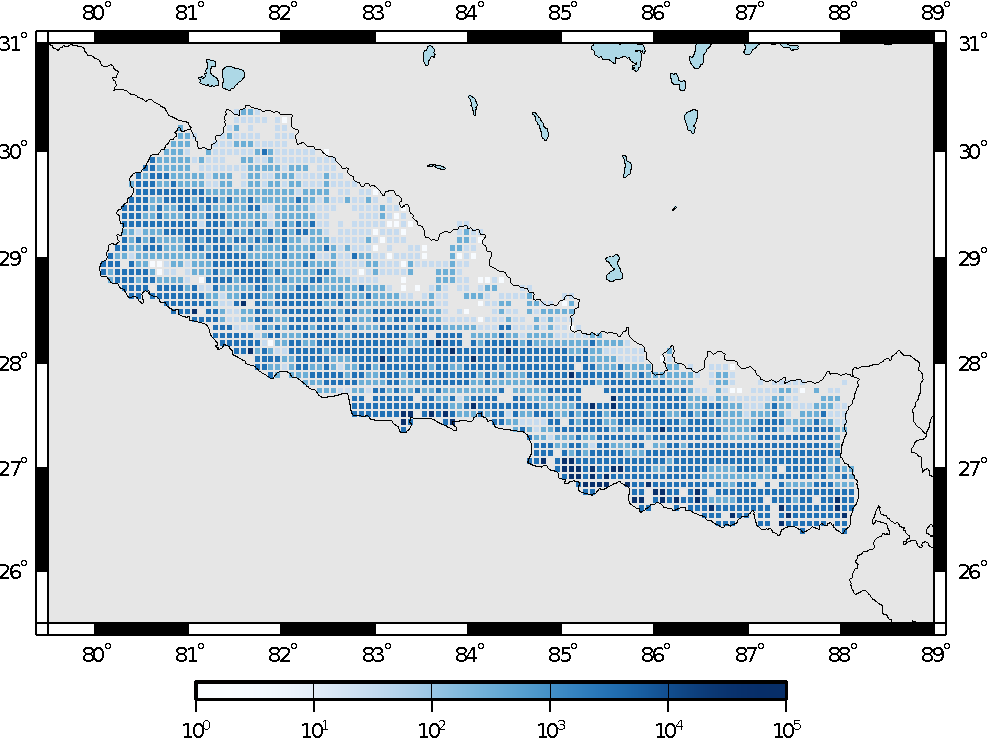
\includegraphics[width=12cm,height=8cm]{figures/risk/exposure-nepal.pdf}
\caption{Distribution of number of buildings in Nepal}
\label{fig:exposure-nepal}
\end{figure}

The building portfolio was organised into four classes for the rural areas
(adobe, dressed stone, unreinforced fired brick, wooden frames), and five
classes for the urban areas (the aforementioned typologies, in addition to
reinforced concrete buildings). For each one of these building typologies,
\glspl{vulnerabilityfunction} and \glspl{fragilityfunction} were collected
from the published literature available for the region. These input models are
only for demonstrative purposes and for further information about the building
characteristics of Nepal, users are advised to contact the National Society
for Earthquake Technology of Nepal (NSET -
\href{http://www.nset.org.np/}{http:www.nset.org.np/}).

The following sections include instructions not only on how to run the risk
calculations, but also on how to produce the necessary hazard inputs. Thus,
each demo comprises the configuration file, \gls{exposuremodel} and fragility or
vulnerability models fundamental for the risk calculations. Each demo folder
also a configuration file and the input models to produce the relevant hazard
inputs.


\section{Scenario Damage Demos}
\label{sec:demos_scenario_damage}
A rupture of magnitude Mw 7 in the central part of Nepal is considered in this
demo. The characteristics of this rupture (geometry, dip, rake, hypocentre,
upper and lower seismogenic depth) are defined in the \verb+fault_rupture.xml+
file, and the hazard and risk calculation settings are specified in the
\verb+job.ini+ file.

To run the Scenario Damage demo, users should navigate to the folder where the
required files have been placed and employ following command:

\begin{minted}[fontsize=\footnotesize,frame=single,bgcolor=lightgray]{shell-session}
user@ubuntu:~\$ oq engine --run job_hazard.ini,job_risk.ini
\end{minted}

The hazard calculation should produce the following outputs:

\begin{minted}[fontsize=\footnotesize,frame=single,bgcolor=lightgray]{shell-session}
Calculation 8967 completed in 4 seconds. Results:
  id | name
9060 | gmf_data
9061 | realizations
\end{minted}

and the following outputs should be produced by the risk calculation:

\begin{minted}[fontsize=\footnotesize,frame=single,bgcolor=lightgray]{shell-session}
Calculation 8968 completed in 16 seconds. Results:
  id | name
9062 | dmg_by_asset
9063 | losses_by_asset
\end{minted}


\section{Scenario Risk Demos}
\label{sec:demos_scenario_risk}
The same rupture described in the Scenario Damage demo is also used for this
demo. In this case, a combined job file, job.ini, is used to specify the
configuration parameters for the hazard and risk calculations.

To run the Scenario Risk demo, users should navigate to the folder where the
required files have been placed and employ following command:

\begin{minted}[fontsize=\footnotesize,frame=single,bgcolor=lightgray]{shell-session}
user@ubuntu:~\$ oq engine --run job.ini
\end{minted}

and the following outputs should be produced:

\begin{minted}[fontsize=\footnotesize,frame=single,bgcolor=lightgray]{shell-session}
Calculation 8970 completed in 16 seconds. Results:
  id | name
9070 | gmfs
9071 | realizations
9072 | loss_map-rlzs
9073 | agglosses-rlzs
\end{minted}


\section{Classical Probabilistic Seismic Damage Demos}
\label{sec:demos_classical_damage}
The seismic source model developed within the Global Seismic Hazard Assessment
Program (GSHAP) is used with the \cite{chiou2008} ground motion prediction
equation to produce the hazard input for this demo. No uncertainties are
considered in the seismic source model and since only one GMPE is being
considered, there will be only one possible path in the logic tree. Therefore,
only one set of seismic hazard curves will be produced. To run the hazard
calculation, the following command needs to be employed:

\begin{minted}[fontsize=\footnotesize,frame=single,bgcolor=lightgray]{shell-session}
user@ubuntu:~\$ oq engine --run job_hazard.ini
\end{minted}

which will produce the following sample hazard output:

\begin{minted}[fontsize=\footnotesize,frame=single,bgcolor=lightgray]{shell-session}
Calculation 8971 completed in 34 seconds. Results:
  id | name
9074 | hcurves
9075 | realizations
\end{minted}

The risk job calculates the probabilistic damage distribution for each asset
in the \gls{exposuremodel} starting from the above generated hazard curves. The
following command launches the risk calculations:

\begin{minted}[fontsize=\footnotesize,frame=single,bgcolor=lightgray]{shell-session}
user@ubuntu:~\$ oq engine --run job_risk.ini --hc 8971
\end{minted}

and the following sample outputs are obtained:

\begin{minted}[fontsize=\footnotesize,frame=single,bgcolor=lightgray]{shell-session}
Calculation 8972 completed in 16 seconds. Results:
  id | name
9076 | damages-rlzs
9077 | damages-stats
\end{minted}


\section{Classical Probabilistic Seismic Risk Demos}
\label{sec:demos_classical_risk}
The same hazard input as described in the Classical Probabilistic Damage demo
is used for this demo. Thus, the workflow to produce the set of hazard curves
described in Section~\ref{sec:demos_classical_damage} is also valid herein.
Then, to run the Classical Probabilistic Risk demo, users should navigate to
the folder containing the demo input models and configuration files and employ
the following command:

\begin{minted}[fontsize=\footnotesize,frame=single,bgcolor=lightgray]{shell-session}
user@ubuntu:~\$ oq engine --run job_hazard.ini
\end{minted}

which will produce the following hazard output:

\begin{minted}[fontsize=\footnotesize,frame=single,bgcolor=lightgray]{shell-session}
Calculation 8971 completed in 34 seconds. Results:
  id | name
9074 | hcurves
9075 | realizations
\end{minted}

In this demo, loss exceedance curves for each asset and two probabilistic loss
maps (for probabilities of exceedance of 1\% and 10\%) are produced. The
following command launches these risk calculations:

\begin{minted}[fontsize=\footnotesize,frame=single,bgcolor=lightgray]{shell-session}
user@ubuntu:~\$ oq engine --run job_risk.ini --hc 8971
\end{minted}

and the following outputs are expected:

\begin{minted}[fontsize=\footnotesize,frame=single,bgcolor=lightgray]{shell-session}
Calculation 8973 completed in 16 seconds. Results:
  id | name
9077 | loss_curves-stats
9078 | loss_maps-stats
9079 | avg_losses-stats
\end{minted}


\section{Event Based Probabilistic Seismic Risk Demos}
\label{sec:demos_event_based_risk}
This demo uses the same probabilistic seismic hazard assessment (PSHA) model
described in the previous examples in Section~\ref{sec:demos_classical_damage}
and Section~\ref{sec:demos_classical_risk}. However, instead of hazard curves,
sets of ground motion fields will be generated by the hazard calculation of
this demo. Again, since there is only one branch in the logic tree, only one
set of ground motion fields will be used in the risk calculations. The hazard
and risk jobs are defined in a single configuration file for this demo. To
trigger the hazard and risk calculations the following command needs to be
used:

\begin{minted}[fontsize=\footnotesize,frame=single,bgcolor=lightgray]{shell-session}
user@ubuntu:~\$ oq engine --run job.ini
\end{minted}

and the following results are expected:

\begin{minted}[fontsize=\footnotesize,frame=single,bgcolor=lightgray]{shell-session}
Calculation 8974 completed in 229 seconds. Results:
  id | name
9079 | agg_curve-rlzs
9080 | agg_loss_table
9081 | loss_maps-rlzs
9082 | rcurves-rlzs
9083 | realizations
9084 | sescollection
\end{minted}


\section{Retrofit Benefit-Cost Ratio Demos}
\label{sec:demos_benefit_cost}
The loss exceedance curves used within this demo are produced using the
Classical Probabilistic Risk calculator. Thus, the process to produce the
seismic hazard curves described in Section~\ref{sec:demos_classical_risk} can
be employed here. Then, the risk calculations can be initiated using the
following command:

\begin{minted}[fontsize=\footnotesize,frame=single,bgcolor=lightgray]{shell-session}
user@ubuntu:~\$ oq engine --run job_risk.ini --hc 8971
\end{minted}

Alternatively, the hazard and risk jobs can be run sequentially using:

\begin{minted}[fontsize=\footnotesize,frame=single,bgcolor=lightgray]{shell-session}
user@ubuntu:~\$ oq engine --run job_hazard.ini,job_risk.ini
\end{minted}

which should produce the following output:

\begin{minted}[fontsize=\footnotesize,frame=single,bgcolor=lightgray]{shell-session}
Calculation 8976 completed in 14 seconds. Results:
  id | name
9087 | Benefit Cost Ratios
\end{minted}

   \cleardoublepage


%-------------------------------------------------------------------------------
%  BIBLIOGRAPHY
%-------------------------------------------------------------------------------

\chapter*{Bibliography}
\addcontentsline{toc}{chapter}{\textcolor{darkgray}{Bibliography}}
\section*{Books}
\printbibliography[heading=bibempty,type=book]
\section*{Articles}
\printbibliography[heading=bibempty,type=article]
\section*{Other Sources}
\printbibliography[heading=bibempty,nottype=book,nottype=article]
\cleardoublepage

%-------------------------------------------------------------------------------
%  INDEX & GLOSSARY
%-------------------------------------------------------------------------------

\printindex
\chapter*{Glossary}
\addcontentsline{toc}{chapter}{\textcolor{darkgray}{Glossary}}
\printglossary[type=acronym, title=List of Acronyms]
\printglossary[title=List of Terms]
\hfill \\ \thispagestyle{empty} \clearpage % ---------------- Final empty page -

\end{document}
